\renewcommand{\textbf}[1]{#1}

\chapter{Onde está o laboratório e os seus cientistas?}
\label{capitulo1}

\epigrafe{%
A Pesquisa é a zona para a qual são arrastados humanos e não humanos, onde ao longo das eras foi feito o mais extraordinário dos experimentos coletivos para distinguir, em tempo real, o ``cosmos'' da ``desordem'' sem que ninguém, cientista ou ``estudioso da ciência'', pudesse saber de antemão qual seria a resposta provisória. Talvez, afinal das contas, os estudos de ciência sejam Anticiência.}%
{Bruno Latour, \textit{A ciência em ação: como seguir cientistas e engenheiros sociedade afora}, 2011.}

Antes de entrar em campo, situo o leitor sobre o que vai encontrar neste capítulo~\ref{capitulo1}. Parto de uma pergunta, onde está o laboratório dos pesquisadores de inteligência artificial e onde estão os seus cientistas, e a desdobro em três gestos analíticos que organizam o capítulo: o corte que delimita uma rede que de outro modo se daria a ver como infinita, a descrição das existências parciais que se compõem comigo e com a inteligência artificial generativa na feitura da tese, e a compostagem que põe a fermentar materiais que o desenho da pesquisa mantinha separados. Ao longo do percurso defino o conceito de tecno-etnografia que dá nome ao trabalho inteiro, sustento a figuração têxtil do método pelo \textit{patchwork}, e fecho o capítulo com a relação entre as duas figurações que constituem esta tese, a têxtil e a topológica, e com a questão que ela me deixou em aberto. A linha do tempo e o mapa que abrem o capítulo dão a ver, antes da leitura, esse percurso e as suas condições. A linha do tempo (Figura~\ref{fig:linha-tempo-cap1}) inscreve, num diagrama de Gantt, os fatos que correm por baixo da pesquisa ao longo de uma década, das condições tecnológicas, sanitárias, regulatórias e bibliométricas às etnográficas, das quais só as últimas se tornam texto enquanto as demais permanecem como condição de possibilidade. O mapa do capítulo (Figura~\ref{fig:mapa-cap1}) dá a ver a arquitetura argumentativa: os fundamentos etnográficos na base, os quatro movimentos em que desdobro os três gestos analíticos, com a matriz dos cortes que cada capítulo da tese faz, e as relações que ligam um movimento ao seguinte. Os dois pertencem ao registro da inscrição, e dão à visão, numa superfície plana, o que penso e teço na espessura do argumento.

Em dezembro de 2022, estive no México para participar do congresso da \textit{Society for Social Studies of Science} (4S), onde apresentei pela primeira vez os resultados preliminares desta pesquisa. Além da experiência de conhecer o país e participar de um evento internacional na área de estudos sociais da ciência e tecnologia, viajei com um grupo diverso de pesquisadores e amigos que contribuíram para aprofundar a reflexão sobre o que significa fazer ciências sociais e investigar como a ciência é produzida em outros áreas do conhecimento. Clarissa, uma das companheiras da viagem e do doutorado na Unicamp, investigava um tema muito diferente sobre o trabalho de antropólogas que menstruam em campo. Ainda assim, compartilhávamos uma preocupação: a ideia de ``não ferir os sentimentos estabelecidos'', uma reflexão de Isabelle Stengers,\footnote{Stengers propõe em \textit{Another Science is Possible} uma ``ciência lenta'' (\textit{slow science}) como resistência às pressões de produtividade que degradam a qualidade do pensamento científico \parencite{stengers2018another}. A defesa da lentidão pressupõe condições de autonomia que nem sempre são possíveis. Esta tese documenta como a temporalidade acadêmica pode se tornar condição de vulnerabilidade quando articulada às lógicas temporais corporativas. Enquanto universidades públicas operam em horizontes de décadas, corporações decidem em ciclos de curto prazo segundo lógicas de retorno sobre investimentos. A capa da edição inglesa traz um caracol, imagem que ressoa com o lema zapatista ``lento, pero avanzo'' e que esta tese adota na dedicatória.} ``como estratégia para criar alianças com interlocutores cientistas, engenheiros e áreas afins''. Longe de se configurar como atitude conformista, trata-se justamente do oposto: ``uma postura calcada apenas no confronto e na denúncia das mazelas da tecnociência é infrutífera, pois produz um resultado alienante e perverso: oculta para nós, pessoas que pesquisam desde as ciências humanas, nossa responsabilidade enquanto coabitantes desse mesmo espaço onde estão os cientistas que denunciamos'' \parencite[p. 314]{costa2024manchando}. Isso não significa que as denúncias sejam irrelevantes, mas ``reconhecer nossa responsabilidade como coabitantes do sistema de produção de conhecimento científico é também aprender a construir e sustentar diálogos, por mais difíceis que sejam'' \parencite[p. 314]{costa2024manchando}.\footnote{Costa desenvolve o conceito de \textit{armadilha} como estratégia metodológica e política para que corpos marcados produzam conhecimento crítico dentro de estruturas acadêmicas sem serem devorados por elas. A armadilha opera em duas etapas, primeiro, encanta através da beleza estética; depois, revela que as imagens fractais são feitas de sangue menstrual, vazando questões feministas de forma que não sejam imediatamente rejeitadas. A etnografia também pode operar como armadilha. Seguir os atores sem julgamento prévio, ganhar confiança, descrever o que é dito e feito para depois tornar visíveis tensões e contradições que os próprios atores não nomeiam \parencite{costa2024manchando}.}

Quase três anos depois do congresso no México, em novembro de 2025, a IBM fechou seu laboratório de pesquisa no Brasil, o único da América Latina, operando há 15 anos com mais de 100 pesquisadores. Em dezembro de 2025, encerrou-se o convênio \texttt{C4AI-IBM}.\footnote{Adoto nesta tese a convenção tipográfica de marcar em fonte monoespaçada, via comando \texttt{\textbackslash texttt\{\}} do \texttt{LaTeX}, três famílias de nomes próprios técnicos: plataformas, linguagens de programação e ambientes computacionais que medeiam a escrita desta tese (\texttt{Python}, \texttt{LaTeX}, \texttt{Overleaf}, \texttt{GitHub}, \texttt{claude code}, \texttt{claude.ai}, \texttt{MermaidChart}, \texttt{NotebookLM}); siglas institucionais de centros, projetos e instituições que compõem o campo de pesquisa (\texttt{C4AI}, \texttt{NLP2}, \texttt{GrIA}, \texttt{USP}, \texttt{FAPESP}, \texttt{IBM}, \texttt{Unicamp}, \texttt{SciELO}, \texttt{Capes}); e nomes próprios de sistemas, modelos e corpora de inteligência artificial (\texttt{Spira}, \texttt{Carolina}, \texttt{Sabiá}, \texttt{claude}, \texttt{GPT}, \texttt{BERT}). A marcação não é questão de estilo. Em coerência com o que sustento sobre figurações como tropos materiais-semióticos no sentido proposto por Donna Haraway, a fonte monoespaçada permanente mantém visível, em toda página do texto, que cada um desses nomes próprios designa um ponto de mediação técnica com agência sobre o que vejo, leio, escrevo e descrevo. A distinção tipográfica entre o redondo, reservado aos nomes próprios de pessoas humanas (Marcelo Finger, Bruno Latour, eu), e a fonte monoespaçada, reservada aos nomes próprios técnicos, recusa a homogeneização tipográfica que apagaria a heterogeneidade dos atores que compõem a rede sociotécnica desta pesquisa.} Desde o início desta pesquisa eu me perguntava até quando aquilo duraria. Na época, havia expectativa por parte do \texttt{C4AI} de que se estendesse por dez anos. Acabou em cinco. A confiança com que meus interlocutores falavam sobre a participação da \texttt{IBM} e a solidez dos investimentos exemplifica de um modo brutal a ``economia especulativa de promessas'' que Stengers critica \parencite{stengers2018another}. Eu, no entanto, repetia para mim mesma: é uma empresa, quero dizer, funciona através de lógicas muito distintas das da universidade. 

Eu já estava na fase final da escrita desta tese quando o convênio foi encerrado, e isso obrigou-me a rever algumas questões que atravessam esta pesquisa. No entanto, acabou por ser também um presente etnográfico sobre o registro de uma parceria público-privada controversa, tensa, contraditória e, a seu modo, bem-sucedida na pesquisa em IA em uma universidade pública brasileira. Essa situação me aproximou do estudo de \textcite{Latour1993Aramis} sobre o Aramis, um sistema de transporte que nunca chegou a existir. Latour fez sua pesquisa entre dezembro de 1987 e janeiro de 1989 com o intuito de investigar por que o projeto havia sido cancelado em fevereiro de 1987.\footnote{Minha posição temporal distingue-se: iniciei a pesquisa em março de 2022, quando a parceria parecia consolidada; o encerramento em dezembro de 2025 não estava previsto. Registrei processos enquanto ocorriam, capturando tensões que permaneciam latentes porque a rede ainda resistia.} Tanto o Aramis quanto o \texttt{C4AI} são casos de parcerias público-privadas onde atores com interesses diversos mobilizam promessas de longo prazo que se desfazem quando cálculos estratégicos corporativos mudam. Em fevereiro de 1987, a Matra distribuiu uma nota ordenando ``pare tudo''; em agosto de 2025, a \texttt{IBM} comunicou internamente que o convênio não seria renovado. No Aramis, a retirada resultou no cancelamento completo após quase vinte anos de investimentos públicos.\footnote{O que restou do Aramis foi um protótipo no saguão da empresa, uma casca vazia sem trilhos, sem eletricidade, sem passageiros: ``um objeto de museu'' antes mesmo de ter sido um objeto no mundo. Latour pergunta quando uma tecnologia se torna um objeto. ``Nunca'', ele responde, ``exceto quando porções extraídas da instituição são colocadas em exposição dentro de museus técnicos'' \parencite[p. 9]{Latour1993Aramis}. É só no ferro-velho que um objeto técnico finalmente se torna objeto. Antes disso, é sempre uma instituição, uma rede de humanos e não humanos, uma transação em curso. Law radicaliza esse argumento ao propor vocabulário para pensar objetos que nunca alcançam fechamento, investigando ``as vidas incertas e complexas dos objetos em um mundo onde não há fechamento'' \parencite[p. 59]{Law2004After}. Objetos são múltiplos mesmo quando parecem singulares, e essa multiplicidade persiste sem se resolver com estabilização.}
No \texttt{C4AI}, a saída da \texttt{IBM} não acabou com o Centro, mas forçou sua reconfiguração como a perda de financiamento corporativo, incertezas sobre projetos em andamento e o esvaziamento das expectativas construídas ao longo de cinco anos. O Centro continua a existir, mas a parceria \texttt{IBM}-\texttt{C4AI} tornou-se objeto do passado; uma relação que deixou rastros em artigos científicos, infraestrutura computacional e promessas não cumpridas. Esta tese começou como uma etnografia de um arranjo sociotécnico aparentemente estável e terminou descrevendo justamente a sua instabilidade e mudanças em um campo volátil e de difícil acesso, e o que isso pode vir a dizer sobre a pesquisa pública em IA no Brasil.

Em 2016, uma cena que circulou amplamente pela internet tornou-se uma das imagens de referência da história recente da inteligência artificial: Jensen Huang, presidente da Nvidia, entrega a Elon Musk, então cofundador da \texttt{OpenAI}, o primeiro supercomputador DGX-1, e Musk assina o chassi da máquina.\footnote{A cena foi registrada em fotografia compartilhada pelo próprio Musk no Twitter, plataforma que viria a adquirir em 2022 e renomear como X, e circulou amplamente desde então. O DGX-1, entregue no escritório da \texttt{OpenAI} em São Francisco, foi avaliado em US\$~129.000 e reunia oito GPUs Tesla P100 com capacidade de até 170 teraflops (FP16), tornando-se a primeira infraestrutura de computação dedicada exclusivamente ao treinamento de redes neurais em escala. Ao fundo da fotografia, uma inscrição parcialmente legível na parede anuncia que o destino do mundo depende do uso que se faz do conhecimento. Opto por não reproduzir a imagem nesta tese e por descrever a cena, em coerência com a economia de figuras que adoto no capítulo. Fonte: Twitter/@elonmusk, 2016.} Menos de uma década depois, a arquitetura de treinamento inaugurada por aquela máquina produziria sistemas capazes de gerar texto, imagem, código e voz com fluência suficiente para redesenhar mercados de trabalho, práticas científicas, sistemas educacionais e disputas geopolíticas. Treinar esses sistemas exige acesso a dezenas, centenas ou milhares de GPUs; a infraestrutura que a cena de 2016 inaugura tornou-se condição de entrada para qualquer laboratório que pretenda produzir modelos competitivos, e a busca por mais poder computacional e mais dados funcionou, por anos, como lei não escrita do desenvolvimento de modelos de linguagem. Em janeiro de 2026, o lançamento do \textit{DeepSeek}, modelo chinês que atingiu desempenho comparável aos sistemas americanos de ponta com apenas uma fração dos recursos computacionais e dos dados, abalou esse paradigma e reabriu a questão sobre quais são, afinal, as condições necessárias para fazer pesquisa em IA. O \texttt{Spira}, projeto desenvolvido no laboratório de processamento de linguagem natural do IME-USP antes mesmo de o \texttt{C4AI} existir como instituição, chegou a essa condição por outra via através de uma doação pontual de GPU da própria Nvidia, registrada nos agradecimentos do primeiro artigo do projeto \parencite{Casanova2021DeepLearning}, sem contrato nem vínculo institucional. O \texttt{C4AI}, por sua vez, manteve ao longo de cinco anos um cluster de GPUs financiado pela USP-Fapes-IBM; em dezembro de 2025, dias após o fim da parceria com a \texttt{IBM}, a USP inaugurou o JAIRU, o maior \textit{cluster} (conjunto de GPUs que trabalham em paralelo) de IA da América Latina, com 96 GPUs Nvidia B200 e um investimento de aproximadamente R\$~40 milhões. As possibilidades que se abriram com aquela máquina são inseparáveis dos problemas que trouxeram, a concentração de poder computacional em poucas corporações, a dependência infraestrutural de países periféricos, a extração de trabalho não remunerado de milhões de usuários cujos dados alimentam os modelos, a opacidade dos sistemas e dificuldade de responsabilização quando erram, entre outros problemas. 

Esta etnografia foi feita durante esses acontecimentos. Iniciei o trabalho de campo no \texttt{C4AI} em março de 2022, seis meses antes do lançamento do \texttt{ChatGPT}, quando a inteligência artificial generativa ainda era objeto de especialistas e o debate público sobre seus efeitos mal havia começado. Entre março de 2022 e dezembro de 2025, assisti, dentro e a partir do Centro, à aceleração que converteu modelos de linguagem em infraestrutura cotidiana, ao crescimento das publicações sobre processamento de linguagem natural pelo \texttt{C4AI}, ao surgimento do primeiro modelo de linguagem brasileiro, à aprovação do primeiro marco regulatório global e ao encerramento da parceria que havia dado origem ao campo que eu estudava. O \texttt{C4AI}, fundado quatro anos depois do DGX-1 com recursos públicos brasileiros e co-financiado pela \texttt{IBM}, é um nó nessa rede e herdeiro das possibilidades, limites e todo o tipo de problema que a fotografia de Jensen Huang e Elon Musk evoca. Acompanhar esse Centro por quase quatro anos é também acompanhar uma pergunta que a fotografia enseja: qual é o papel da universidade pública na produção de conhecimento em inteligência artificial quando quem está nas fronteiras da pesquisa em IA são essas mesmas corporações? Esta tese documenta uma tentativa de resposta situada à essa questão: o que o \texttt{C4AI} fez, como se organizou e o que ficou quando a \texttt{IBM} deixou de co-financiar o centro. 

\begin{figure}[htbp]
  \centering
  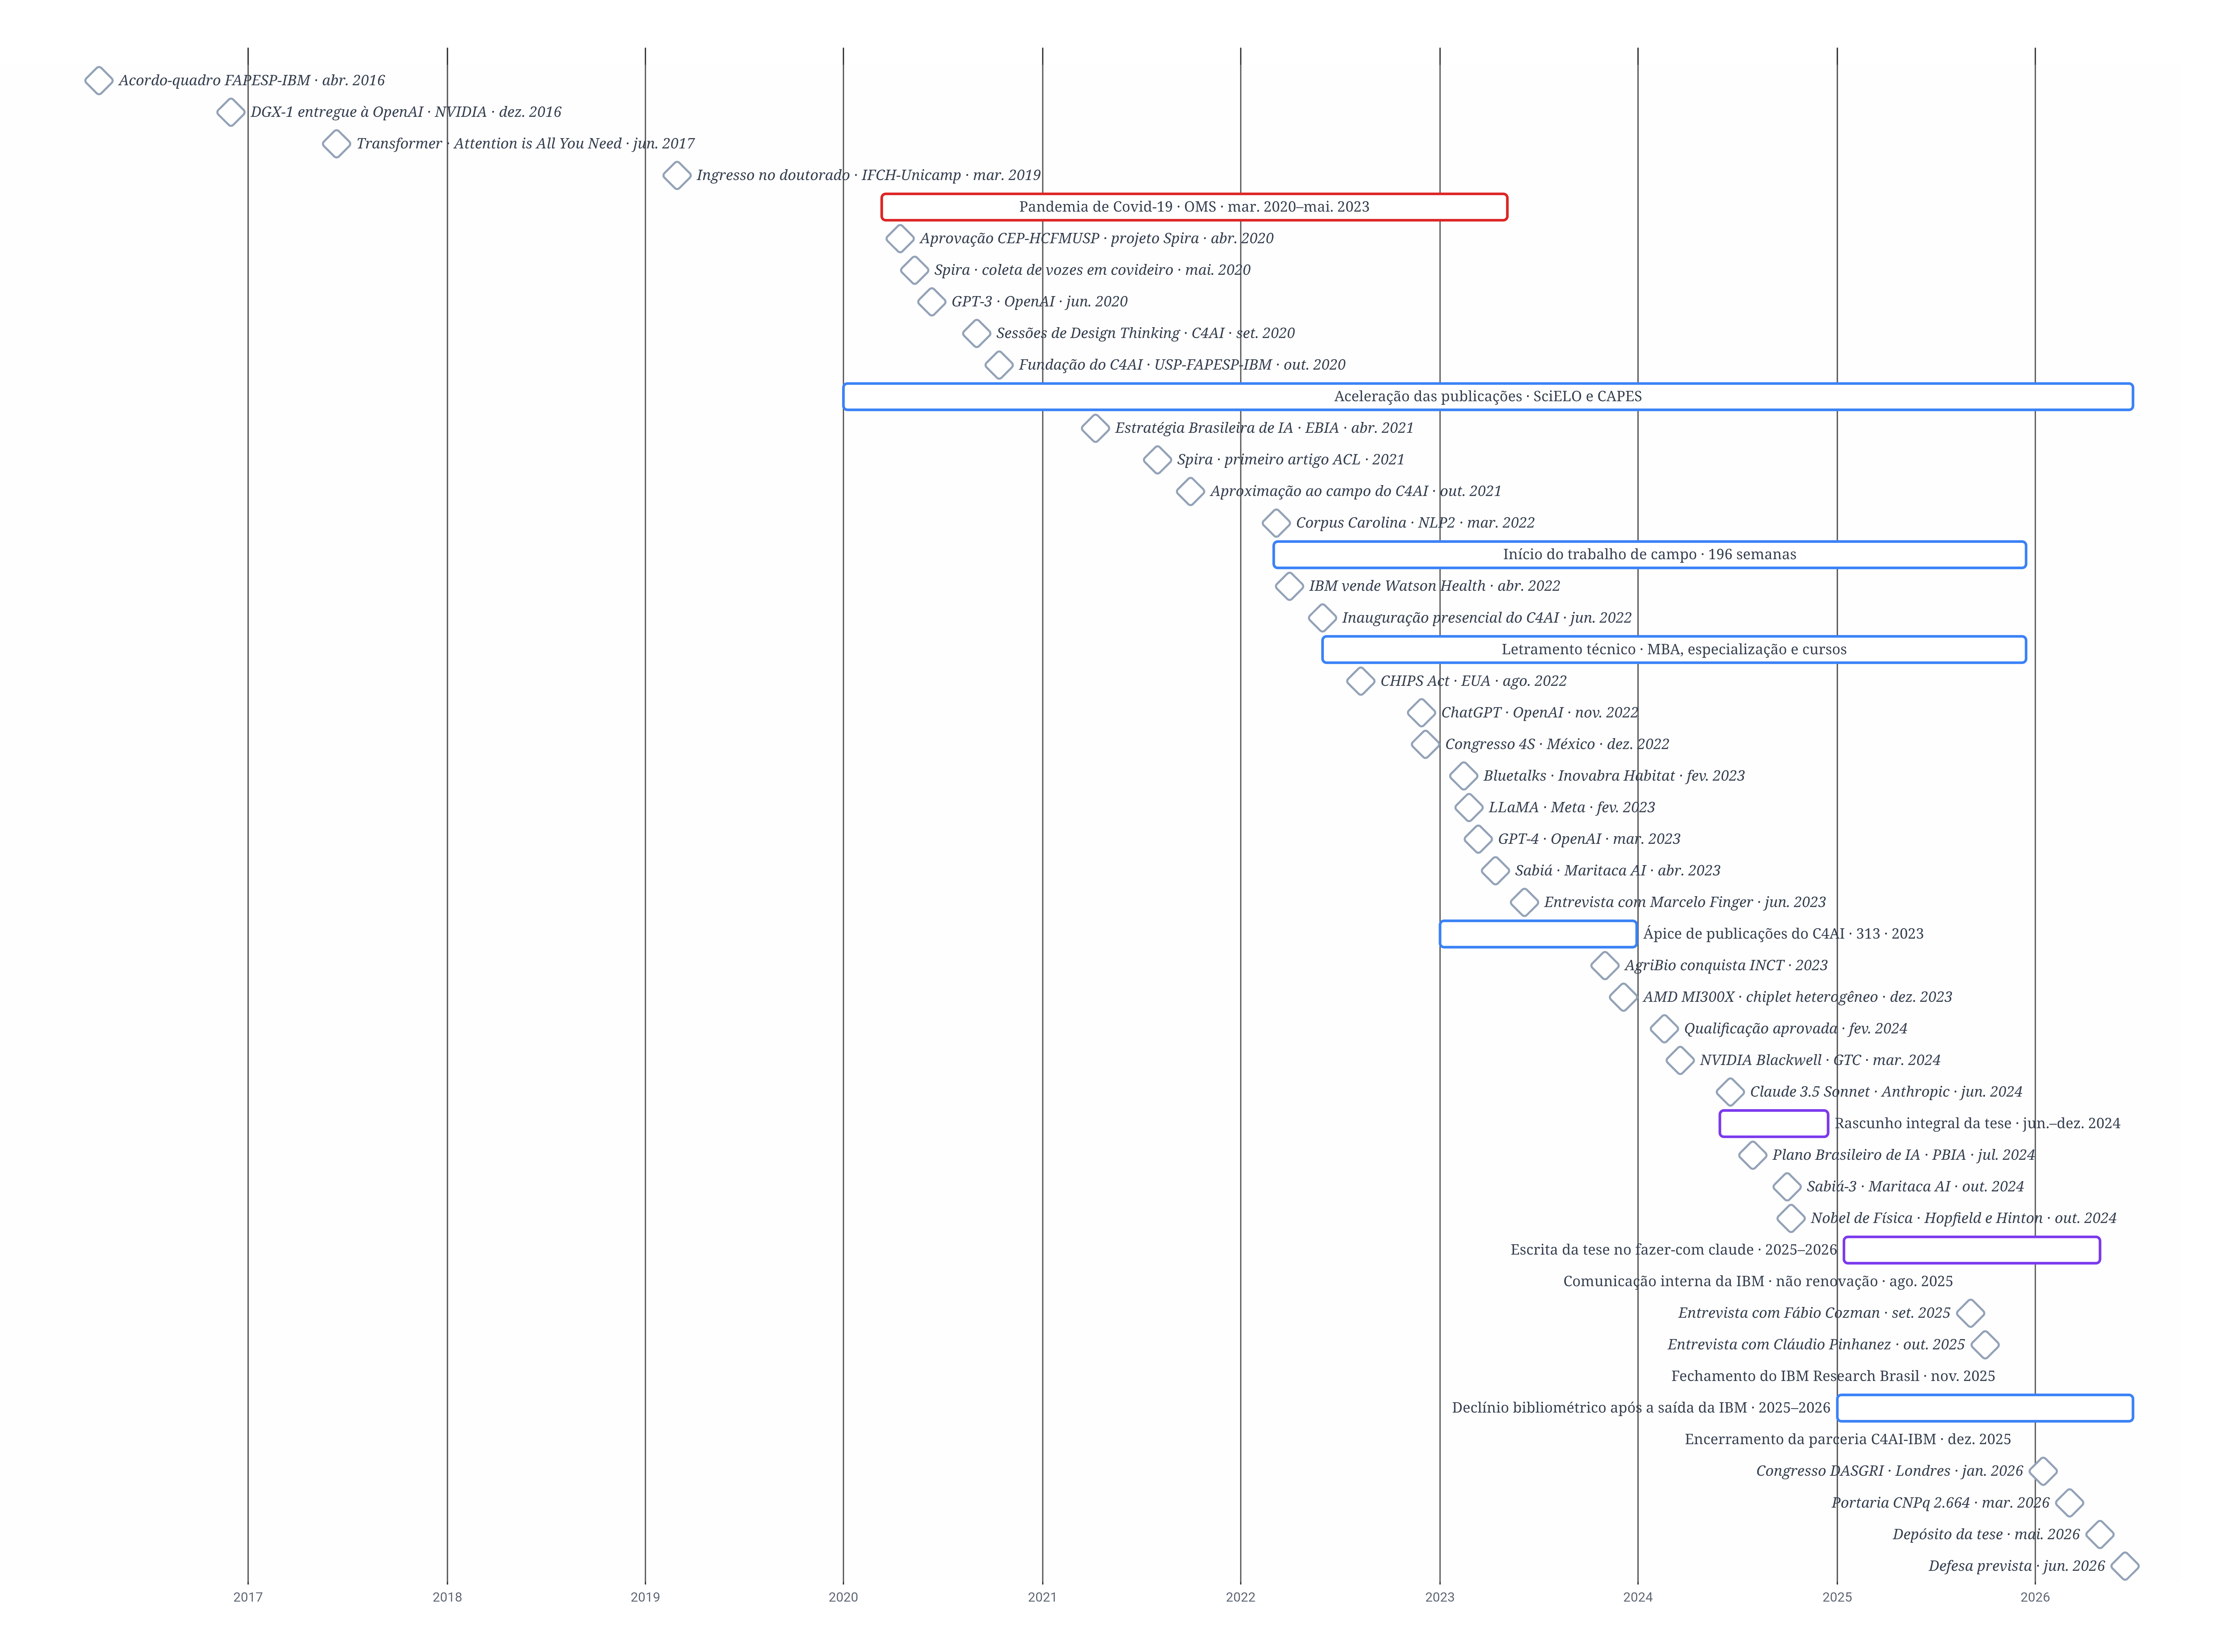
\includegraphics[width=0.7\textwidth,keepaspectratio]{figuras/cap.1/linha-tempo-capitulo1.png}
  \caption[Linha do tempo do capítulo~\ref{capitulo1}]{\textbf{Linha do tempo do capítulo~\ref{capitulo1}: condições materiais, sanitárias, regulatórias, bibliométricas e etnográficas em que se fez esta pesquisa.} Esta linha do tempo dá a ver, numa superfície plana, os fatos que correm por baixo do texto da tese, dispostos em sequência ao longo de uma década, e pertence ao registro da inscrição, no sentido de \textcite{Latour1986Visualization}. Leio-a, em diálogo com \textcite{Law2004After}, como o \textit{hinterland} que sustenta o que aparece como presença no texto: a maior parte desses fatos permanece como condição de possibilidade, e só os do trabalho de campo se tornam texto. Atravessam a cronologia as condições \textit{tecnológicas}, da aceleração da infraestrutura computacional para IA entre 2016 e 2026, do DGX-1 entregue à \texttt{OpenAI} à arquitetura Blackwell da NVIDIA, e dos modelos que cruzaram minha pesquisa, GPT-3, \texttt{ChatGPT}, GPT-4, LLaMA, Sabiá e Sabiá-3 da \texttt{Maritaca AI}, o \texttt{claude} 3.5 Sonnet e modelos da família Opus, com o Nobel de Física de 2024 para Hopfield e Hinton; as \textit{sanitárias}, da pandemia de Covid-19 entre março de 2020 e maio de 2023, condição de possibilidade do \texttt{Spira}, que coletou vozes em covideiro, e do \texttt{C4AI}, fundado em outubro de 2020, em plena pandemia; as \textit{regulatórias}, da aprovação ética do CEP-HCFMUSP para o \texttt{Spira} em abril de 2020 às políticas científicas brasileiras de fomento à IA (EBIA 2021, PBIA 2024), aos arranjos internacionais que reposicionaram o setor (CHIPS Act, AI Act) e à Portaria CNPq 2.664 de 2026, que minha tese antecipou por escolha metodológica; as \textit{bibliométricas}, da aceleração das publicações em IA nas ciências humanas brasileiras (SciELO, CAPES) entre 2020 e 2026, com o ápice de 313 publicações do \texttt{C4AI} em 2023 e o declínio associado à saída da \texttt{IBM} em 2025-2026; e as \textit{etnográficas}, os fatos que se tornam texto na tese, do acordo-quadro Fapesp-IBM de 2016 ao meu ingresso no doutorado em 2019, à fundação do \texttt{C4AI} em outubro de 2020, à minha aproximação ao campo em outubro de 2021, às 196 semanas de trabalho de campo entre março de 2022 e dezembro de 2025, ao letramento técnico acumulado em paralelo, ao rascunho integral da tese redigido entre junho e dezembro de 2024 sem assistência de inteligência artificial, ao fazer-com \texttt{claude} e à \textit{skill} \texttt{juliane-dissertacao} entre janeiro de 2025 e maio de 2026, às três entrevistas com Marcelo Finger, Fábio Cozman e Cláudio Pinhanez, e aos dois eventos que abriram a caixa-preta institucional na finalização da pesquisa, o fechamento da \texttt{IBM} Research Brasil em novembro de 2025 e o encerramento da parceria \texttt{C4AI}-\texttt{IBM} em dezembro de 2025. Inscrição que produzi no fazer-com \texttt{claude} (\texttt{Anthropic}) e hospedei no \texttt{MermaidChart}\footnote{Versão interativa do diagrama disponível em: \url{https://mermaid.ai/d/b27ca78c-b037-42fe-a3eb-939a092e1455}. Acesso em: \today.}, em que os fatos que o texto principal precisou deixar fora para sustentar seu fluxo narrativo se dispõem, todos, numa só superfície. Esta linha do tempo é o par do mapa do capítulo (Figura~\ref{fig:mapa-cap1}): onde o mapa inscreve a estrutura argumentativa do capítulo, a linha do tempo inscreve as condições materiais que correm por baixo dela.}
  \label{fig:linha-tempo-cap1}
\end{figure}

\begin{figure}[htbp]
  \centering
  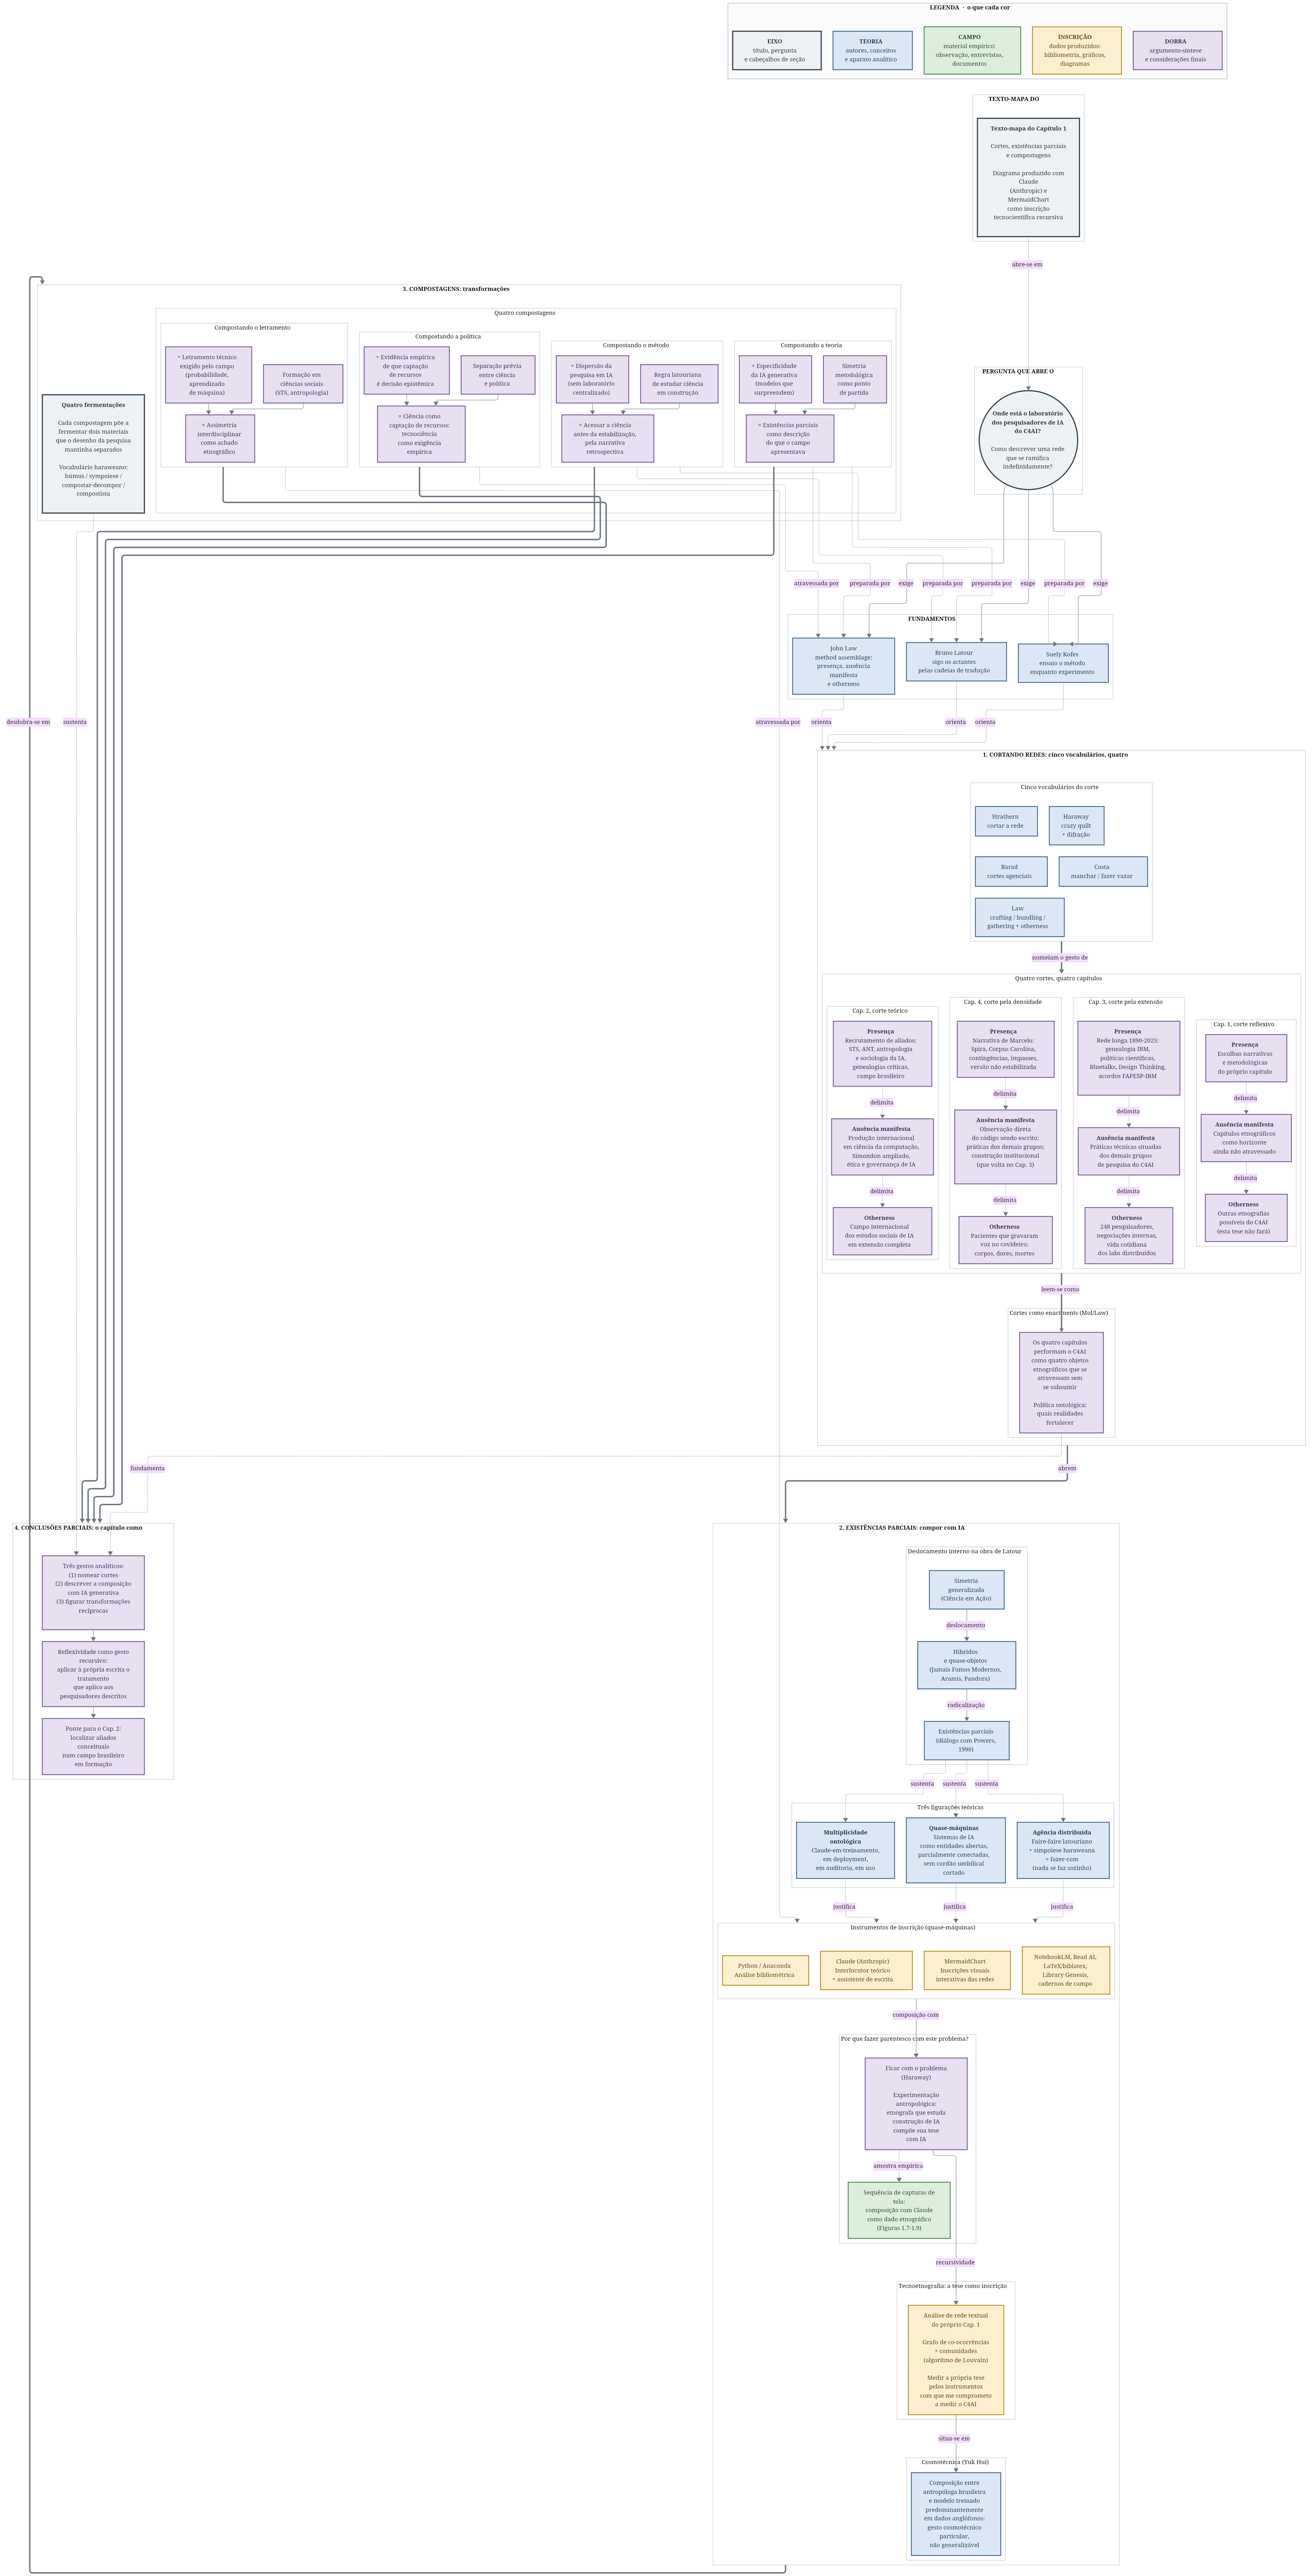
\includegraphics[width=0.4\textwidth]{figuras/cap.1/mapa-capitulo1-v2.png}
  \caption[Mapa do capítulo~\ref{capitulo1}]{\textbf{Mapa do capítulo~\ref{capitulo1}: a arquitetura argumentativa, da pergunta inicial às conclusões parciais.} Este mapa situa o leitor na arquitetura do capítulo, ao dar a ver numa superfície plana os fundamentos etnográficos que o sustentam, os quatro movimentos em que desdobro os três gestos analíticos, e as relações que ligam um movimento ao seguinte. Na base, três fundamentos sustentam o restante: \textcite{Kofes2015Maconaria}, para quem o método se ensaia enquanto se experimenta, \textcite{Latour2011CienciaEmAcao}, que pede para seguir os actantes, e \textcite{Law2004After}, com o \textit{method assemblage} que produz presença, ausência manifesta e \textit{otherness}. O primeiro movimento, \textit{Cortando redes}, reúne o corte de Strathern e conceitos vizinhos de Barad, Haraway, Costa e Law e a matriz dos quatro cortes que cada capítulo da tese faz, descrito cada um pela tríade presença/ausência manifesta/\textit{otherness}, e que se leem como \textit{enactments} no sentido praxiográfico de \textcite{mol2002body} e \textcite{Law2004After}. O segundo, \textit{Existências parciais}, parte de um deslocamento interno na obra de Latour, do princípio de simetria aos híbridos e às existências parciais, e sustenta três figurações teóricas (quase-máquinas, agência distribuída e a multiplicidade ontológica de Claude), que justificam o trabalho dos instrumentos de inscrição com que componho a tese e a análise de rede textual do próprio capítulo como gesto recursivo, situados como gesto cosmotécnico particular (Hui). O terceiro, \textit{Compostagens}, nomeia quatro fermentações específicas, do método, da teoria, do letramento e da política, cada uma como soma de duas matérias que o desenho da pesquisa mantinha separadas. As \textit{Conclusões parciais} reúnem os três gestos analíticos, registram a reflexividade como gesto recursivo e abrem a ponte para o capítulo~\ref{capitulo2}. A inscrição é, ela mesma, parte do que descreve: produzi-a com o \texttt{claude} (\texttt{Anthropic}) e hospedei-a no \texttt{MermaidChart}\footnote{Versão interativa do diagrama disponível em: \url{https://mermaid.ai/d/6dbd9e0b-a652-428d-99b1-a76d0c068b5b}. Acesso em: \today.}, em cadeia de traduções entre minha descrição verbal das relações argumentativas do capítulo e o código \textit{Mermaid} executado pelo modelo. A inscrição funciona, nos termos de \textcite{Latour1986Visualization}, como móvel imutável que torna combinável em superfície plana o que o texto desdobra ao longo de dezenas de páginas, e nos termos de \textcite{Law2004After}, como redução produtiva que perde riqueza empírica e ganha capacidade de fazer conexões.}
  \label{fig:mapa-cap1}
\end{figure}

Estar no campo durante esse período implicou um desafio que vai além do habitual esforço de atualização bibliográfica. Nas seções que se seguem, detalho os fundamentos teórico-metodológicos que orientaram essa trajetória, as operações de triangulação que permitiram articular dados heterogêneos, os cortes analíticos estratégicos que transformaram redes infinitas em objetos etnográficos analisáveis, e as quatro lições que o encontro entre teoria e campo produziu como contribuições metodológicas desta tese. A etnografia, como o caracol, avançou devagar, secretando seu rastro. O que esse rastro deixou está escrito (e inscrito) nesta tese. Mas, esse rastro também deixa meus vestígios enquanto pesquisadora aprendendo a caminhar sobre superfícies estranhas, e deixa, sobretudo, os vestígios dos próprios pesquisadores do \texttt{C4AI} construindo redes, mobilizando inscrições e recrutando aliados, negociando com corporações, fazendo, por fim, \textit{tecnociência}.\footnote{Em \textit{Ciência em Ação}, \textcite{Latour2011CienciaEmAcao} nomeia com esse termo o campo em que ciência e tecnologia se produzem como um só processo, sem partição prévia entre fatos e artefatos. \textcite{stengers2018another} o toma em outra direção, a da \textit{fast science}, e renomeia a economia do conhecimento como \textit{economia especulativa de promessas}.}

Para Latour, a tecnociência é prática coletiva de fechamento de caixas-pretas, em que as controvérsias se resolvem pela capacidade de estender redes em extensão e em densidade, nas quais teoremas, máquinas, documentos, financiamentos e alianças institucionais tornam o custo da discordância proibitivo para o oponente. Stengers descreve a forma que as práticas científicas assumem quando recrutadas pela lógica industrial e pelos imperativos de competitividade, em que a formação do pesquisador funciona como anestesia que o torna insensível à recalcitrância dos mundos atravessados pela pesquisa, e em que a avaliação crítica entre pares se enfraquece porque ninguém quer cortar o galho da promessa que sustenta o campo. Latour e Stengers descrevem dimensões diferentes do mesmo fenômeno: os conceitos latourianos de rede e de translação permitem mapear como redes tecnocientíficas se estendem e se estabilizam; o diagnóstico de Stengers expõe como essas redes, sob condições contemporâneas, vivem regimes específicos de captura, aceleração e despolitização. Sustento esta tese nos dois registros. O que me interessa na proposta de Stengers é que ela articula, ao mesmo tempo, a crítica, que não se reduz à denúncia, e a construção de alianças. A trajetória da parceria \texttt{C4AI}-\texttt{IBM}, com a promessa inicial de dez anos reduzida a cinco quando os cálculos corporativos se reorganizaram, é caso empírico em que as duas leituras se sobrepõem: a rede extensa que Latour permite descrever é também a economia de promessas que Stengers diagnostica. Estudá-las em ação, antes do fechamento que tentam estabilizar e da retirada que pode desfazê-las, é o gesto que orienta a primeira regra metodológica que reproduzo adiante. É desse rastro que trato agora. Para isso, começo por mobilizar a noção de \textit{actante}.\footnote{Tomo a definição em quatro registros: \textcite[p. 127, 138-140]{Latour2011CienciaEmAcao}; \textcite[Glossário]{Latour2017Esperanca}; \textcite[Glossário]{latour2004politics}; e \textcite{johnson1988mixing}. O termo vem da semiótica de Algirdas Julien Greimas, que descrevia com ele qualquer entidade dotada de papel narrativo em um relato, sem prejulgamento sobre sua natureza.}

Latour transporta a generalidade do termo para os estudos de ciência e tecnologia para escapar do antropocentrismo embutido na palavra \enquote{ator}, que tende a pressupor intenção, consciência e personificação. Recolho quatro registros que se complementam e agem juntos nesta tese. Em \textit{Ciência em Ação}, o actante é qualquer pessoa ou coisa que seja representada, sem diferença prática, para a análise, entre representar trabalhadores num sindicato e representar hormônios num experimento, pois uns e outros dependem de porta-vozes que articulem suas posições. Em \textit{A Esperança de Pandora}, a definição se refina em chave pragmática: o actante é definido pela lista de provas a que é submetido e pelas performances que apresenta nelas, e a sua competência ou essência se deduz só depois, a partir do que conseguiu fazer ou impedir, como o microrganismo que, antes de receber nome, é apenas a soma das vitórias e derrotas que registra ao transformar açúcar em álcool, resistir à fervura, sobreviver a antissépticos. Em \textit{Políticas da Natureza}, a ênfase desloca-se para a relacionalidade, e o actante é qualquer entidade que modifica outra entidade em uma prova; a agência nunca é propriedade isolada, é \textit{fait-faire}, fazer-fazer distribuído entre os mediadores da rede. No artigo sobre o dispositivo de fechamento automático de portas, Latour acrescenta a distinção que importa para a descrição etnográfica: actantes podem ser figurativos, quando aparecem personificados, ou não figurativos, quando agem de modo técnico ou abstrato, como uma mola, um quebra-molas, um algoritmo. O que define o actante é o que ele faz na cadeia de associações, não o tipo de entidade que parece ser.

Tratar humanos e não humanos como actantes não afirma a sua equivalência ontológica nem dissolve as diferenças entre os seus modos de agir; recusa a partição prévia que decidiria, antes da pesquisa, quem age e quem é apenas cenário. Os actantes que me importam nesta tese são, em sua maioria, entidades que transformam, traduzem e tensionam aquilo que atravessam, em contraste com os intermediários, que apenas transportam sem alteração. Contratos, modelos computacionais, GPUs, vozes gravadas em enfermarias, o vírus SARS-CoV-2 e linguagens formais entram nas redes que descrevo porque deslocam o curso das associações em que participam, e tornam possível fazer coisas que antes eram impossíveis ou ocorriam de outro modo.

Esse conceito sustenta a noção de simetria teórico-metodológica que, em geral, orienta a teoria ator-rede. Considerando a interpretação de um de seus principais formuladores, Bruno Latour, por exemplo, argumenta que não devemos aceitar acriticamente o que os cientistas dizem sobre a Natureza, tampouco o que os cientistas sociais dizem sobre a Sociedade. A sua quarta regra metodológica estabelece que ``uma vez que a resolução de uma controvérsia é a causa da estabilidade da sociedade, não podemos usar a sociedade para explicar como e por que uma controvérsia foi resolvida. Devemos considerar simetricamente os esforços para alistar e controlar recursos humanos e não-humanos'' \parencite[p. 225]{Latour2011CienciaEmAcao}. Isso desloca Natureza e Sociedade da posição de causas explicativas do desfecho das controvérsias para a posição de consequências estabilizadas ao final do processo. Para esta tese, essa regra tem implicação metodológica direta: não posso explicar a pesquisa em inteligência artificial no \texttt{C4AI} recorrendo a fatores sociais externos como se fossem mais estáveis ou mais reais do que os algoritmos, os dados ou os modelos. Em outras palavras, devo observar empiricamente quem ou o que efetivamente \enquote{age} em determinada situação, não esquecendo também de como e para quê no sentido de Haraway e Stengers. 

O título desta tese, \textit{tecno-etnografia de um centro de inteligência artificial}, nomeia o gesto que organiza minha pesquisa em sua totalidade e que se desdobra em quatro tramas, uma em cada capítulo. \textit{Tecnoetnografia} é o conceito que surge da indissociabilidade entre escrita, análise e técnicas que desenvolvi nesta pesquisa \textit{sobre} e \textit{com} inteligência artificial, em uma posição em que objeto de pesquisa e infraestrutura de pesquisa compartilham natureza técnica. O termo tem antecedentes nos estudos de ciência e tecnologia, e o sentido em que o cunho aqui é específico: nomeia a indissociabilidade entre estudar inteligência artificial em uma universidade pública brasileira durante o intervalo histórico em que a IA generativa se tornou infraestrutura cotidiana, e estudar com inteligência artificial, dado que essa mesma IA passou a participar das condições materiais da minha escrita acadêmica.\footnote{A subseção~\ref{subsec:tecnoetnografia} desenvolve a filiação do conceito à etnografia digital de \textcite{Pink2016DigitalEthnography} e a inflexão que ele introduz.} O uso composto de \textit{tecno-} com \textit{etnografia} circula desde os anos 2000 em dois registros, o da etnografia de objetos técnicos e práticas tecnocientíficas, em continuidade com a etnografia de laboratório, e o da etnografia digital, voltada a comunidades \emph{online} e a interações mediadas por tela. O sentido em que o cunho recolhe os dois e acrescenta uma camada que decorre do fazer-com modelos de linguagem generativos: a tecno-etnografia é, aqui, etnografia da tecnociência feita em parceria explícita com a tecnologia descrita, em diálogo reflexivo e situado que documenta a participação dessa tecnologia nas condições de possibilidade da pesquisa. O termo é, nesse sentido, herdado e tensionado pela própria prática que ele nomeia.

Cada um dos quatro capítulos desta tese desdobra a tecno-etnografia em uma trama distinta, com escala e materialidade próprias. Neste capítulo~\ref{capitulo1}, a tecno-etnografia se faz como gesto recursivo sobre a própria escrita etnográfica: estudo inteligência artificial usando inteligência artificial para inscrever e descrever as redes que tornam o estudo possível, e a subseção~\ref{subsec:tecnoetnografia} apresenta as seis inscrições tecnocientíficas que produzi para fazer a análise textual do próprio texto que estava escrevendo. Essa análise, que faço em parceria com o \texttt{claude code}, converte o capítulo em rede de co-ocorrência de termos, por uma análise de rede textual, e segue a trajetória dos conceitos ao longo da escrita, para que eu possa ver o que pesa, o que se liga a quê e o que persiste no texto que costurei. No capítulo~\ref{capitulo2}, a tecno-etnografia se desdobra em duas linhas internas: a análise das metáforas e figurações na obra de Bruno Latour (e de Latour e Woolgar em \emph{Laboratory Life}), que faço com o \texttt{claude code} por uma análise lexicométrica sobre seis livros e artigos publicados entre 1986 e 2013, e o mapeamento da emergência do campo brasileiro de estudos em inteligência artificial nas ciências humanas e sociais, que faço com o \texttt{claude} por análise bibliométrica das plataformas \texttt{SciELO} e \texttt{Capes}. As duas linhas mobilizam as referências que cada uma convoca conforme o objeto que recortam, e os objetos das quatro tramas, por mais distintos que pareçam, derivam todos do mesmo gesto de pôr as coisas em relação. As duas análises do capítulo~\ref{capitulo2} são parentes da análise textual que faço neste capítulo~\ref{capitulo1}, e diferem dela no que tomam por objeto e no instrumento que aplicam. A análise deste capítulo~\ref{capitulo1} é reflexiva e indutiva, ou seja, recai sobre a minha própria escrita e deixa as comunidades de termos emergirem do texto sem catálogo prévio. A análise das figurações no capítulo~\ref{capitulo2} é dirigida e dedutiva, isto é, recai sobre a obra de um terceiro, Latour, e aplica a ela um catálogo de campos figurais que construí antes da análise, para investigar qual figuração domina cada obra e como esse domínio se desloca. No capítulo~\ref{capitulo3}, a tecno-etnografia se faz como descrição da rede do \texttt{C4AI} pela sua extensão: a parceria \texttt{USP}-\texttt{FAPESP}-\texttt{IBM} ao longo de cinco anos, do convênio inicial em outubro de 2020 ao encerramento em dezembro de 2025, com a genealogia corporativa da \texttt{IBM} estendida desde Hollerith em 1890, em capítulo composto em parceria com a inteligência artificial generativa que tematizo como infraestrutura. No capítulo~\ref{capitulo4}, a tecno-etnografia se faz em sua forma mais recursiva: o \texttt{Spira}, sistema de detecção de insuficiência respiratória desenvolvido durante a pandemia, é objeto de inteligência artificial descrito em tese composta com inteligência artificial, e a cadeia de inscrição da voz humana ao espectrograma processado pela rede neural se desdobra em capítulo que faz da IA simultaneamente sujeito, objeto e infraestrutura da minha descrição. Em todos os quatro capítulos, a parceria com o \texttt{claude} e o \texttt{claude code} comparece como dado etnográfico tematizado, e os repositórios públicos no \texttt{GitHub} onde versiono os \emph{scripts}, catálogos e \emph{outputs} de cada análise são a forma material em que a indissociabilidade entre escrita, análise e técnicas se inscreve em registro auditável linha a linha. As quatro tramas se atravessam sem se subsumir umas às outras, e a tecno-etnografia que esta tese ensaia se completa quando as quatro tramas se costuram entre si nos termos em que cada capítulo as desdobra.

O desafio desse tipo de posicionamento analítico consiste em se apoiar no arcabouço teórico-metodológico das ciências sociais e, simultaneamente, voltar esses mesmos conceitos, centrais às investigações sociológicas e antropológicas, para a própria análise. Isso exige uma suspensão recorrente das nossas próprias crenças enquanto cientistas sociais, suspensão que precisa ser refeita a cada nova passagem do texto e que se torna condição para o aprendizado, para um aprender antropologicamente no sentido proposto por \textcite{Ingold2019Antropologia}. É nesse ponto que a análise alcança sua maior densidade, porque os actantes mobilizados nesta tese vão de políticas científicas e contratos institucionais a GPUs, algoritmos, vozes humanas gravadas em enfermarias, inscrições tecnocientíficas dos artigos (imagens microscópicas, diagramas, gráficos, equações) e o próprio vírus SARS-CoV-2. Os capítulo s 3 e 4 documentam como esses actantes se associam em cadeias heterogêneas que dão forma a redes sociotécnicas. Isso ocorre tanto em reuniões de \textit{design thinking}, como meus interlocutores chamam as conversas que decidem os rumos das pesquisas e suas condições, quanto nas enfermarias hospitalares onde pacientes com Covid-19 tiveram suas falas gravadas e convertidas em dados computacionais para treinamento e inferência do \texttt{Spira}. A pandemia atravessa esta tese: o \texttt{C4AI} foi inaugurado em outubro de 2020, em plena crise sanitária, e o trabalho de campo começou em março de 2022, ainda sob seus efeitos. Seguir os atores levou-me ao vírus SARS-CoV-2, que se mostrou um actante que reconfigurou as condições de possibilidade tanto das pesquisas em IA que observo quanto da pesquisa que realizo. Esse posicionamento teórico-metodológico é, no sentido que \textcite{Barad2007Meeting} dá ao termo, ético-onto-epistemológico.\footnote{Como adiantado no capítulo~\ref{capitulo0}, Karen Barad cunha a expressão \enquote{ethico-onto-epistem-ology} para nomear a inseparabilidade entre as questões do que existe, do que se pode conhecer e da responsabilidade que se assume ao conhecer e fazer existir: \enquote{conhecer, pensar, medir, teorizar e observar são práticas materiais de intra-ação no mundo e como parte dele} \parencite[p.~90]{Barad2007Meeting}. A escrita com hífens do termo indica que as três dimensões são inseparáveis em qualquer prática de pesquisa. Para o argumento desta tese, isso significa que tratar simetricamente vírus, GPUs, algoritmos e políticas científicas é, ao mesmo tempo, decisão sobre o que existe, decisão sobre como conhecer e decisão sobre quem responde pelas associações que se estabilizam. O capítulo~\ref{capitulo4} mobiliza essa orientação no plano quando o \textit{pipeline} (representação visual de como foi feito um sistema de IA) do \texttt{Spira} produz, pelo próprio aparato, o objeto que mede, calcula, treina e infere.} Esse esforço, contudo, não está livre de contradições. Em muitos momentos, contradigo a mim mesma e aos princípios que digo seguir. Pensar dessa maneira exige virar uma chave interpretativa que nem sempre conseguimos acionar.
Anos de formação em antropologia e sociologia me ensinaram a buscar o social nos fenômenos, a desconfiar das explicações técnicas, a revelar os interesses ocultos. Desaprender esse costume acadêmico é um trabalho contínuo e necessariamente incompleto. Manter essa disciplina (não poderia ser um tipo de recursividade?) ao longo desta tese é uma prova de força (e não estou falando da mesma prova de força no sentido latouriano, apesar de também ter a ver com isso). Por isso, se o leitor encontrar passagens em que recorro apressadamente a fatores sociais para explicar o que deveria ser descrito em sua heterogeneidade, saiba que estou mais ou menos ciente desses deslizes.

A formulação ético-onto-epistemológica de Barad encontra o seu antecedente operacional, por assim dizer, nas sete regras metodológicas e nos seis princípios que Latour propõe ao final daquela obra. Onde Barad nomeia a inseparabilidade entre o que existe, o que se pode conhecer e a responsabilidade que se assume ao conhecer, Latour elaborou um guia prático para sustentar essa inseparabilidade ao longo de uma pesquisa: o que considerar como objeto, em que momento entrar no campo, como tratar simetricamente humanos e não humanos, o que fazer diante de divisores entre interior e exterior. Reproduzo-os aqui na íntegra porque cada um deles intervém no texto desta tese como decisão tomada a cada novo capítulo, a cada nova entrevista, a cada decisão sobre qual associação seguir e qual deixar fora da análise.

\begin{citacaoabnt}
\textit{Regra 1.} Estudamos a ciência em ação, e não a ciência ou tecnologia pronta; para isso, ou chegamos antes que fatos e máquinas se tenham transformado em caixas-pretas, ou acompanhamos as controvérsias que as reabrem.

\textit{Regra 2.} Para determinar a objetividade ou subjetividade de uma afirmação, a eficiência ou a perfeição de um mecanismo, não devemos procurar por suas qualidades intrínsecas, mas por todas as transformações que ele sofre depois, nas mãos dos outros.

\textit{Regra 3.} Como a solução de uma controvérsia é a causa da representação da Natureza, e não sua consequência, nunca podemos utilizar essa consequência, a Natureza, para explicar como e por que uma controvérsia foi resolvida.

\textit{Regra 4.} Como a resolução de uma controvérsia é a causa da estabilidade da sociedade, não podemos usar a sociedade para explicar como e por que uma controvérsia foi dirimida. Devemos considerar simetricamente os esforços para alistar recursos humanos e não-humanos.

\textit{Regra 5.} Com relação àquilo de que é feita a tecnociência, devemos permanecer tão indecisos quanto os vários atores que seguimos; sempre que se constrói um divisor entre interior e exterior, devemos estudar os dois lados simultaneamente e fazer uma lista (não importa se longa e heterogênea) daqueles que realmente trabalham.

\textit{Regra 6.} Diante da acusação de irracionalidade, não olhamos para que regra da lógica foi infringida nem que estrutura social poderia explicar a distorção, mas sim para o ângulo e a direção do deslocamento do observador, bem como para a extensão da rede que assim está sendo construída.

\textit{Regra 7.} Antes de atribuir qualquer qualidade especial à mente ou ao método das pessoas, examinemos os muitos modos como as inscrições são coligidas, combinadas, interligadas e devolvidas. Só se alguma coisa ficar sem explicação depois do estudo da rede é que deveremos começar a falar em fatores cognitivos \parencite[p. 420-422]{Latour2011CienciaEmAcao}.
\end{citacaoabnt}

Se as regras orientam a prática etnográfica, os seis princípios extraem dela consequências teóricas mais amplas sobre a natureza dos fatos, das máquinas e das redes que os sustentam:

\begin{citacaoabnt}
\textit{Primeiro princípio.} O destino de fatos e máquinas está nas mãos dos consumidores finais; suas qualidades, portanto, são consequência, e não causa, de uma ação coletiva.

\textit{Segundo princípio.} Os cientistas e engenheiros falam em nome de novos aliados que conformaram e alistaram; representantes entre outros representantes, com esses recursos inesperados, fazem o fiel da balança de forças pender em seu favor.

\textit{Terceiro princípio.} Nunca somos postos diante da ciência, da tecnologia e da sociedade, mas sim diante de uma gama de associações mais fracas e mais fortes; portanto, entender o que são fatos e máquinas é o mesmo que entender o que as pessoas são.

\textit{Quarto princípio.} Quanto mais esotérico o conteúdo da ciência e da tecnologia, mais elas se expandem externamente; portanto, 'ciência e tecnologia' é apenas um subconjunto da tecnociência.

\textit{Quinto princípio.} A acusação de irracionalidade é sempre feita por alguém que está construindo uma rede em relação a outra pessoa que atravessa seu caminho; portanto, não há Grande Divisor entre mentes, mas apenas redes maiores ou menores.

\textit{Sexto princípio.} A história da tecnociência é, em grande parte, a história dos recursos espalhados ao longo das redes para acelerar a mobilidade, a fidedignidade, a combinação e a coesão dos traçados que possibilitam a ação a distância \parencite[p. 422-424]{Latour2011CienciaEmAcao}.
\end{citacaoabnt}

Conforme desenvolvia esta pesquisa, orientada por esses princípios e regras, percebi que, ao fazer associações com os pesquisadores do \texttt{C4AI}, tanto eu quanto esta tese passamos a fazer parte das redes do Centro, e tanto eu quanto a tese nos tornamos actantes nessas redes; assim, esta tese tornou-se também uma inscrição tecnocientífica.\footnote{A percepção de que esta tese também fazia redes me foi sugerida por Fernanda Rosa, em conversa após eu apresentar as primeiras impressões desta pesquisa no encontro anual da \textit{Society for Social Studies of Science} (4S), em Cholula, em dezembro de 2022. Fernanda Rosa investiga infraestruturas digitais no Sul Global e aparece também na revisão do capítulo~\ref{capitulo2}. A formulação dela deslocou a posição em que eu me colocava até então: o que eu vinha descrevendo como acompanhamento dos cientistas e engenheiros do \texttt{C4AI} também era construção de associações que iam ganhando forma na medida em que as registrava. Levei tempo para perceber o alcance metodológico daquela formulação, e foi essa percepção que veio a desenhar o eixo desta tese.} Latour define instrumento como qualquer estrutura que possibilite uma exposição visual de qualquer tipo em um texto científico \parencite[p.~102]{Latour2011CienciaEmAcao}, e inscrição como aquilo que esse instrumento produz: o traçado, o gráfico, a tabela, o registro.\footnote{O conceito de inscrição é desenvolvido em três frentes. \textcite[caps.~1--2]{Latour2011CienciaEmAcao} analisa o artigo científico como construção sobre camadas de inscrições e descreve o laboratório como fábrica de inscrições; \textcite[cap.~2]{Latour2017Esperanca} acompanha uma expedição pedológica à Amazônia e mostra como o solo se transforma sucessivamente em amostras, em cores de um código de Munsell, em números e em um diagrama de relatório, cadeia que ele chama de referência circulante; em \enquote{Visualization and Cognition} \parencite{Latour1986Visualization}, define as inscrições como \textit{móveis imutáveis}, condição da dominação à distância. Para que o conhecimento se acumule em centros de cálculo, as inscrições precisam ser móveis, transportáveis dos lugares distantes para o centro; imutáveis, sem distorção no transporte; e combináveis, rearranjáveis em uma única superfície plana. A construção de fatos opera por uma cascata de simplificações: uma substância complexa se reduz a um traço, que se reduz a um número, que se torna média em uma tabela, até chegar a uma afirmação dura em um artigo. No texto científico, a inscrição traz o referente para dentro da narrativa: o autor aponta para a figura e mostra a prova, em vez de pedir que o leitor acredite em sua palavra.} Esta etnografia mobiliza uma série dessas inscrições por meio de imagens, diagramas, gráficos e do site que apresenta e performa esta tese. E quando digo que a tese em si é uma inscrição tecnocientífica, é porque ela possibilita certos tipos de ações. De alguma maneira, traduzi aquele pedaço do mundo envolvendo o \texttt{C4AI} para o formato de papel, ou melhor, para um arquivo digital que começou como anotações em \texttt{.txt} no bloco de notas do celular, passou por um \texttt{.docx} no Word e no \texttt{Google Docs}, depois para \texttt{Latex} no Overleaf, até chegar a um \texttt{.pdf} e, talvez, a um volume encadernado ou a um livro impresso.\footnote{Diferentemente de um texto impresso em papel (que também depende de uma complexa cadeia de técnicas e tecnologias, afinal, até a escrita à mão exige algum suporte físico e um conjunto de habilidades aprendidas ao longo do tempo), um arquivo digital só pode ser compreendido por um dispositivo, como um computador, para que possamos ver as letras na tela. Isso pode parecer um detalhe simples, mas envolve diversas mediações técnicas: o computador lê os diferentes formatos de arquivo convertendo os dados em sequências de bits (0s e 1s, desligado/ligado, falso/verdadeiro) e transformando-os em informações compreensíveis, em um processo que passa pelo sistema operacional, pelas extensões de arquivo e pelos aplicativos específicos instalados na máquina. Sem um software de aplicação que funcione como tradutor dos dados brutos contidos nos arquivos e os transforme em algo compreensível para o usuário, os dados de arquivos como o desta tese em \texttt{.pdf} permanecem apenas como dados crus, isto é, mera eletricidade; e, sem a ação do software, essa eletricidade não pode ser convertida em uma mensagem ou informação inteligível. Por exemplo, o código binário 01000001, para um processador de texto, corresponde à letra \enquote{A}. Não é impressionante o que a computação tornou possível? Quando consideramos os modelos de linguagem, tudo isso fica ainda mais interessante, porque esses modelos funcionam em uma escala de indeterminação, ao contrário de qualquer outro sistema computacional tradicional, e aliás contra as suas próprias bases fundacionais que opera segundo lógicas de determinação e continuidade. Arrisco sugerir que é justamente essa indeterminação e descontinuidade que torna a inteligência artificial tão instigante para a antropologia. Por mais que se tente controlar tais aspectos por meio dos famosos \textit{prompts} (como ficaram conhecidas as instruções que são feitas à IA generativa), eles não serão totalmente eliminados. O \textit{prompt} expressa, em certo sentido, a ilusão frustrada de que seria possível controlar integralmente esses sistemas. Isso não significa que esses sistemas sejam incontroláveis, mas talvez os \textit{prompts} não sejam a melhor forma de fazê-lo. Eu mesma realizei experimentações e considerei o resultado tão bizarro em tentar impedir que o sistema falhasse, cometesse erros ou reproduzisse suas marcas estilísticas características; pareceu-me que a IA foi assim \enquote{desumanizada} de uma vez por todas.} Esse recorte dizia respeito a algo muito maior do que eu, no qual se desenrolavam acontecimentos que só podiam ser notados a partir de uma certa escala de análise, incluindo não humanos invisíveis ao olhar humano sem a mediação da tecnociência, como o coronavírus. Ao mobilizar inscrições de diversos tipos, a tese transforma eventos dispersos no tempo e no espaço em traçados estáveis, combináveis e transportáveis. À medida que essa rede se expande para além do Centro, associando actantes cada vez mais inesperados e heterogêneos, a tese adquire o status do que Latour denomina inscrição também literária. É essa inscrição que permite à tecnociência agir à distância e converter fenômenos complexos, remotos ou invisíveis em um arquivo digital que pode ser lido, interpretado, analisado, isto é, dominado, medido, controlado, utilizado tanto para apreciação quanto para persuadir outros acerca da realidade de um fato tecnocientífico cujas cadeias de associações ganham força conforme a extensão da rede e o número de elementos que ela consegue associar \parencite{Latour2011CienciaEmAcao}, ou fazer alianças \parencite{stengers2010cosmopolitics1}.

\section{Etnografias: fazendo o método a partir da experiência}
\label{sec:etnografia-heterodoxa}

\epigrafe{%
Há muitos métodos para o estudo da construção de fatos científicos e artefatos técnicos. A primeira regra metodológica pela qual nos decidimos na Introdução é a mais simples de todas. Não tentaremos analisar os produtos finais; em vez disso, seguiremos os passos de cientistas e engenheiros nos momentos e nos lugares nos quais planejam, desfazem, modificam. Vamos dos produtos finais à produção, de objetos instáveis e frios a objetos instáveis e mais quentes. Estar ali \textbf{antes} que a caixa se fechasse e ficasse preta. Com esse método simples precisamos apenas seguir os melhores de todos os guias, os próprios cientistas, em sua tentativa de fechar uma caixa-preta e abrir outra.}%
{Bruno Latour, \textit{A ciência em ação: como seguir cientistas e engenheiros sociedade afora}, 2011.}

Esta pesquisa fundamenta-se em uma acepção específica de etnografia elaborada por Suely Kofes.\footnote{A acepção de etnografia mobilizada nesta tese é a que Suely Kofes desenvolve em \textit{Dilemas na maçonaria contemporânea: um experimento antropológico} \parencite{Kofes2015Maconaria}. A formulação aparece em duas seções complementares do livro: na parte dois, intitulada \enquote{Etnografia heterodoxa}, e na seção final, \enquote{Pesquisa antropológica como método e/ou como experiência} \parencite[pp.~291--303]{Kofes2015Maconaria}. Nessas seções, Kofes articula o entrelaçamento entre biografia, etnografia e antropologia como alternativa às categorizações dicotômicas supostamente universais.
Essa acepção dialoga com obra anterior da autora, \textit{Uma trajetória, em narrativas} \parencite{kofes2001trajetoria}, na qual Kofes contrasta sua proposta com outras definições consolidadas de etnografia: a etnografia como totalidade na formulação de Bronislaw Malinowski em \textit{Argonautas do Pacífico Ocidental}, como trabalho de campo na formulação de Martyn Hammersley e Paul Atkinson em \textit{Ethnography: Principles in Practice}, e como escritura na formulação de James Clifford e George Marcus em \textit{Writing Culture: The Poetics and Politics of Ethnography}. Kofes observa que nenhuma dessas definições dá conta isoladamente de explicar o que faz uma etnógrafa.} A proposta de Kofes é pensar a pesquisa antropológica como método e como experiência, formulação que ela desenvolve no capítulo final do livro de 2015 ao fazer dialogar Strathern, Favret-Saada e Turner. Kofes parte de uma desconfiança sobre a verdade do empirismo como método e da consciência dos limites do método: o que está em jogo é a relação entre pesquisa de campo, escrita e teoria, e a posição da etnógrafa nessa relação \parencite[pp.~298, 300]{Kofes2015Maconaria}. Mobilizando Marilyn Strathern, Kofes situa a etnografia como prática reveladora ou \enquote{revelatória}, que convida o leitor a considerar o que não é revelado na evidência do que o é \parencite[p.~297]{Kofes2015Maconaria}. Com Jeanne Favret-Saada, sustenta que a etnógrafa precisa entrar no processo da palavra e se tornar uma falante como outra, posicionar-se no e como discurso, e ao escrever os resultados retornar à situação de enunciação, fazendo desse vai e vem entre a tomada inicial e sua retomada teórica o objeto mesmo da reflexão \parencite[p.~299]{Kofes2015Maconaria}.\footnote{A formulação que Suely Kofes recupera de Jeanne Favret-Saada vem de \textit{Les mots, la mort, les sorts: la sorcellerie dans le Bocage} \parencite[p.~32]{FavretSaada1977}, etnografia da feitiçaria no Bocage francês na qual a autora reconstrói a posição da etnógrafa como interna ao processo de enunciação que descreve. O argumento de Favret-Saada se desdobra em ensaio posterior, \enquote{Être affecté}, publicado originalmente na revista \textit{Gradhiva} e mais tarde recolhido em \textit{Désorceler} \parencite{FavretSaada1990SerAfetado}, no qual a autora formula a categoria do \enquote{ser afetado} como modalidade epistemológica específica da etnografia, distinta da observação participante e da empatia identificatória. A tradução brasileira desse ensaio, feita por Paula Siqueira Lopes e Tânia Stolze Lima, está disponível em \textit{Cadernos de Campo} \parencite{FavretSaada2005SerAfetado}, edição que torna acessível ao leitor brasileiro a formulação metodológica que Favret-Saada sintetiza retrospectivamente sobre a pesquisa do Bocage.} Essa posição encontra eco no que Strathern descreve como recriação imaginativa dos efeitos do próprio campo, gesto que torna a escrita antropológica parte do nexo entre pesquisa e teoria \parencite[p.~299]{Kofes2015Maconaria}. É a partir dessa sequência argumentativa que Kofes recupera Victor Turner: a tensão entre método e experiência se torna desnecessária quando dissolvida pela dramatização narrativa \parencite[p.~301]{Kofes2015Maconaria}. A experiência, ao se expressar narrativamente, conecta eventos e afecções e lhes confere significações e valores; essa expressão narrativa da experiência é o que Turner chama de \textit{structured unit of experience}, unidade estrutural da experiência. A narrativa, ao ligar o que se concebe como cesura, cria uma estrutura de relação, a estrutura de experiência. É por isso que a narrativa da etnógrafa é parte do método: o método se ensaia conforme se experimenta, e só pode ser narrado retrospectivamente porque se constitui junto com o objeto, no encontro de campo.\footnote{A formulação de Suely Kofes ressoa com o conceito de \textit{method assemblage} proposto por John Law em \textit{After Method: Mess in Social Science Research} \parencite{Law2004After}. Ambas as formulações recusam a normatividade prévia dos métodos convencionais, embora por vias distintas: Law aponta para a multiplicidade das realidades que o método produz e para a inseparabilidade entre o método e os mundos que ele torna pensáveis; Kofes sustenta a recusa pela via da experiência, argumentando que o método se ensaia através da experiência, inclusive da experiência de campo, e que a escrita antropológica é parte constitutiva desse ensaio \parencite[pp.~298--299]{Kofes2015Maconaria}.}

A formulação que Kofes recupera de Strathern tem nome próprio na obra da antropóloga, o efeito etnográfico.\footnote{O efeito etnográfico (\textit{the ethnographic effect}) nomeia, em Strathern, o momento da escrita em que o material da pesquisa de campo é retomado e produz relações que não estavam dadas no campo. A escrita etnográfica cria, nesse sentido, um segundo campo, e a relação entre esse segundo campo e o campo da observação permanece parcial, dado que cada um toca o outro sem o abranger \parencite[pp.~7, 345]{strathern2014efeito}. A distinção entre evocar e representar vem de \textit{Partial Connections} \parencite[p.~7]{strathern2005partial}. A ficção persuasiva, que Strathern desenvolve a propósito da contextualização na antropologia de Malinowski, toma \textit{ficção} em sentido de fabricação, no eco do que Gillian Beer observa sobre a teoria em estado de esboço, sentido alheio ao de falsidade \parencite[p.~173]{strathern2014efeito}.} Strathern sustenta que a escrita etnográfica cria um segundo campo, distinto do campo da observação e tão gerador de conhecimento quanto ele, e que os dois se tocam parcialmente sem que um abranja o outro. A escrita funciona como recriação imaginativa de alguns dos efeitos da pesquisa de campo, e Strathern a situa no registro da evocação, em contraste com a representação que tomaria o texto como espelho do que se observou. O efeito etnográfico se dá nesse momento da escrita, em que observação e análise se relacionam no mesmo plano. Strathern descreve ainda a descrição etnográfica como uma ficção persuasiva, ficção no sentido de fabricação literária que organiza e justapõe ideias para transmiti-las ao leitor. Reconhecer a escrita como segundo campo dá nome ao que faço quando tomo esta tese como inscrição tecnocientífica: o texto que componho sobre o \texttt{C4AI} é um campo em que observação e análise se relacionam no mesmo plano, e a tecno-etnografia que ensaio neste capítulo~\ref{capitulo1} faz desse segundo campo o seu objeto, ao tomar a própria escrita, feita com \texttt{claude.ai}, como dado etnográfico.

Essa concepção de etnografia como pesquisa antropológica que articula método e experiência dialoga com a teoria ator-rede de maneiras que interessam a esta tese. Primeiro, porque recusa categorias dicotômicas supostamente universais, como a separação entre humano e não humano. Segundo, porque trata o campo como processo de aprendizado: assim como Latour propõe que sigamos os atores sem decidir de antemão o que é técnico e o que é social, Kofes propõe que o método se ensaia conforme nos deixamos afetar pelo encontro com nossos interlocutores. Terceiro, porque ambas as abordagens organizam-se em torno das inscrições, dos documentos, das narrativas, dos artefatos e dos traçados que constituem simultaneamente nossos dados e nossos modos de produzir conhecimento.

A etnobiografia, desdobramento metodológico que Kofes formula \parencite{kofes2001trajetoria}, também pode ser uma forma de investigar instituições, como faço nesta tese. Kofes adota o conceito de pessoa, em vez do de indivíduo, a partir de Marilyn Strathern, para quem a pessoa abriga o potencial para relações e é, ela própria, constituída por uma matriz de relações sociais, de sociabilidade, conforme exposto em \textit{Property, Substance and Effect} \parencite{strathern2000pse}.\footnote{A concepção de pessoa que Suely Kofes mobiliza em diálogo com Marilyn Strathern parte de uma formulação relacional da pessoa, desenvolvida pela autora a partir de sua etnografia na Melanésia. Em \textit{The Gender of the Gift: Problems with Women and Problems with Society in Melanesia} \parencite{strathern1988gender}, Strathern formula a pessoa como microcosmo de relações sociais, constituída pelas ações de outros, alimentação, cuidados, trocas, e capaz de destacar partes de si para criar novas relações. O argumento aprofunda-se em \textit{Property, Substance and Effect: Anthropological Essays on Persons and Things} \parencite{strathern2000pse} e em \textit{Partial Connections} \parencite{strathern2005partial}. Strathern designa essa pessoa como \textit{dividual}, entidade compósita e partível: na economia da dádiva melanésia, as pessoas trocam perspectivas, e o que circula nas trocas são porções de pessoa incorporadas em substâncias e objetos. A formulação contrasta com a noção euro-americana de indivíduo como unidade atômica e indivisível, que se completa pela posse de si mesmo. Strathern propõe pensar a pessoa como circuito de conexões parciais, em que cada parte estende a outra sem encerrar-se em uma identidade unitária final. Quando Kofes recorre a essa formulação para sustentar sua etnobiografia, transporta para o registro etnográfico a superação da pessoa como entidade preexistente à sociedade onde vive: a pessoa, e por extensão a etnógrafa e o coletivo etnografado, é o efeito momentâneo de uma matriz de relações que a constitui. A tradução brasileira dos ensaios de Strathern sobre o efeito etnográfico está disponível em coletânea \parencite{strathern2014efeito}, edição que torna acessível ao leitor brasileiro o conjunto de elaborações sobre o que Strathern chama de efeito etnográfico.} Se, como Kofes, é possível fazer a etnobiografia de uma Loja maçônica, então é igualmente possível fazer a etnobiografia de um centro de pesquisa em inteligência artificial. Isso significa reconstruir a trajetória e a vida de um coletivo, abrangendo suas práticas e estruturas, suas fundações e refundações, suas alianças e rupturas, suas transformações ao longo do tempo. Assim, o \texttt{C4AI} é também um actante cuja biografia se entrelaça com a minha trajetória de pesquisadora, e nesse entrelaçamento ressoa a formulação de Roy Wagner que Kofes recupera no mesmo capítulo: todo entendimento de uma outra cultura é um experimento com a nossa própria \parencite[p.~296]{Kofes2015Maconaria}. Esse gesto abre a possibilidade de pensar como cientistas e engenheiros fazem inteligência artificial a partir das mediações que a etnografia e a teoria ator-rede tornam visíveis nesta pesquisa.

Essa formulação ressoa com a atenção de Latour aos porta-vozes e às cadeias de tradução. Assim como o cientista no laboratório fala em nome de entidades que não podem falar por si mesmas, a antropóloga fala em nome de interlocutores cujas vozes são traduzidas, editadas, recontextualizadas no texto final. A responsabilidade dessa tradução é constitutiva do trabalho antropológico tanto quanto do trabalho científico. Concretamente, baseio-me em técnicas qualitativas diversas: observação de eventos acadêmicos e corporativos, entrevistas semiestruturadas com líderes de grupos de pesquisa, análise documental de acordos institucionais e acompanhamento de atividades de divulgação científica, de forma presencial ou remota. Essa diversidade de fontes caracteriza o que Kofes chama de pesquisa artesanal: trabalho que articula observação rigorosa e registro documental com a sensibilidade da experiência antropológica. Os dados desta tese provêm de conjunto de observações, escuta, conversas, anotações, entrevistas e convivência com pessoas ligadas ao Centro ao longo de quase quatro anos (março de 2022 a dezembro de 2025). A parceria \texttt{C4AI}-\texttt{IBM} foi inaugurada em outubro de 2020, antes do início do meu trabalho de campo. O que acompanhei diretamente é o período que vai de março de 2022 em diante; o intervalo anterior, de 2020 a 2022, eu o reconstituí pelas entrevistas e pelos relatórios institucionais, e é como reconstrução documental, e não como observação, que ele entra nesta tese. A articulação entre a observação direta a partir de 2022, as entrevistas e os documentos que cobrem o período 2020--2025 me permitiu seguir o arranjo da fundação à dissolução, parte por presença em campo, parte por rastros que pude consultar. Entrevistei Fábio Cozman em setembro de 2025 e Cláudio Pinhanez em outubro de 2025, antes do anúncio público do encerramento; em nenhuma das duas entrevistas o fim da parceria foi mencionado. A não-renovação só se tornou pública depois, no anúncio que Cláudio publicou no \texttt{LinkedIn} em 20 de novembro de 2025. Releio hoje aquelas entrevistas sabendo do desfecho que então eu não conhecia, e é dessa posição retrospectiva, a minha, que descrevo o que registrei, sem atribuir aos meus interlocutores um saber sobre o futuro do arranjo que eu não poderia verificar.
 
A imersão prolongada exigiu também aprendizado de linguagens e códigos específicos. Assim como Kofes precisou decifrar a grafia e as abreviaturas maçônicas, precisei aprender a linguagem dos pesquisadores em inteligência artificial, abrangendo o vocabulário técnico, os modos de argumentar, as hierarquias implícitas entre abordagens e os critérios tácitos de avaliação. Esse processo de alfabetização foi condição de possibilidade para o aprofundamento da inteligência artificial. Mas a ausência inicial de conhecimento especializado teve um impacto duplo. Por um lado, constituiu uma vantagem metodológica, ao tratar a atividade científica como elemento novo, evitei a tendência de adotar antecipadamente a distinção entre social e técnico. Por outro lado, trouxe vulnerabilidade quando o foco mudou para a necessidade de aprender com os cientistas. Foi assim que compreendi, por exemplo, que o laboratório do cientista da computação é o computador, ideia aparentemente óbvia mas que possui implicações que merecem atenção. O computador, portátil e móvel, é mais do que simples objeto ou mediador: é o próprio laboratório, um actante, ponto na rede e simultaneamente também uma rede. Mas essa mobilidade tem limites que só se tornam visíveis quando a infraestrutura falha ou exige intervenção. Latour observa que objetos técnicos, enquanto funcionam, são intermediários silenciosos e mudos; é a crise, a quebra, o mau funcionamento, que revela sua existência, suas partes e sua agência \parencite[cap.~6]{Latour2017Esperanca}.\footnote{Em 4 de março de 2026, Luciano Antonio Digiampietri, pesquisador do Grupo de Pesquisa em Inteligência Artificial da EACH-USP (GrIA), fundado em 2006 e que divide com o \texttt{C4AI} a infraestrutura computacional, publicou no Instagram uma fotografia da placa de entrada do Centro com a legenda: \enquote{Hoje foi dia de presencial no laboratório. (Tive que apertar um botão, no servidor.)} (Digiampietri, 2026, comunicação pessoal). O servidor em questão executa experimentos de IA, hospeda modelos de linguagem e realiza \textit{fine-tuning} para tarefas como detecção de \textit{bots} e identificação de notícias falsas. Luciano acessa o servidor remotamente de sua sala na EACH, a cem metros de distância, da reitoria da USP, ou de sua casa, e seus orientandos também o acessam remotamente. Naquele dia, o servidor desligou e não religou automaticamente, e foi necessário que ele fosse até a máquina para pressionar o botão de reinicialização. Em seguida, voltou a acessá-lo remotamente, da sala a cem metros de distância. A postagem condensa o paradoxo: o laboratório distribuído, que dispensa presença contínua, convocou o corpo do pesquisador para um gesto mínimo e indispensável. Mostra ainda que o \texttt{C4AI} não construiu sua infraestrutura do zero, instalou-se sobre redes já constituídas, como o GrIA, que existia desde 2006. Luciano me explicou o contexto via mensagem privada no Instagram em março de 2026 e autorizou expressamente o uso da postagem e da explicação como dado etnográfico; o termo de consentimento assinado encontra-se em posse da autora.} O laboratório de IA às vezes exige que alguém se desloque até onde as máquinas estão quando elas desligam ou param de funcionar por algum motivo para \enquote{apertar um botão}.

Tanto a teoria ator-rede de Bruno Latour e a etnografia heterodoxa de Suely Kofes funcionam juntos nesta tese porque enfrentam, a partir de temas e questões distintas, o mesmo problema. Latour o formula no registro epistemológico, onde a coerência sobre o que os atores dizem ou fazem deve ser realizada dentro do próprio movimento de associação em que as redes se fazem e se tornam mais fortes ou mais fracas, onde os fatos sempre estarão relacionados ao tamanho de uma rede e da quantidade de suas associações \parencite[p.~331]{Latour2011CienciaEmAcao}. Kofes formula a questão a partir da escrita etnográfica, pela qual o método ensaia-se conforme a etnógrafa se deixa afetar pelo que encontra, e esse ensaio só pode ser narrado retrospectivamente. Em Latour, esse gesto se realiza como seguir os actantes e mapear as redes que eles compõem; em Kofes, como deixar-se afetar pelo encontro de campo e compor a narrativa em que a experiência se estrutura. A própria adoção da teoria ator-rede nesta tese emergiu e foi personalizada de acordo com o processo de escrita, e isso é, na formulação de Kofes, o método ensaiando-se através da experiência. O gesto tem precedente etnográfico em \textit{Vida de Laboratório}, onde \textcite{Latour1997VidaLaboratorio} mostraram que o \textit{hinterland} de instrumentos de inscrição, protocolos experimentais e negociações constitui a própria ciência \parencite[p.~38]{Law2004After}.\footnote{O conceito de \textit{hinterland} é desenvolvido por \textcite[pp.~27--42, 159]{Law2004After} e definido no glossário como \enquote{a bundle of indefinitely extending and more or less routinised and costly literary and material relations that include statements about reality and the realities themselves; a hinterland includes inscription devices, and enacts a topography of reality possibilities, impossibilities, and probabilities. A concrete metaphor for absence and presence} \parencite[p.~159]{Law2004After}. Mantenho o termo em itálico, sem traduzir, ao longo da tese, dado que essa obra não tem tradução brasileira disponível e que nenhuma palavra do português recobre integralmente o campo semântico que Law mobiliza, articulando a imagem geográfica do território interior que abastece um porto sem aparecer nas trocas desse porto, a topografia de possibilidades de realidade encenada por dispositivos de inscrição, e a metáfora concreta para a relação entre presença e ausência. Discuto a aproximação com a palavra \enquote{contexto}, recuperada pela etimologia de \textit{contexere} (tecer junto), na subseção~\ref{subsec:cortando-redes}. Em termos metodológicos, o \textit{hinterland} de uma descrição é o conjunto de práticas, pressupostos, infraestruturas e recursos sedimentados que sustentam o que aparece sem serem tematizados. O conceito é distinto, mas inseparável da noção de \textit{corte}, desenvolvida na subseção~\ref{subsec:cortando-redes} a partir de \textcite{strathern2011cortando}: o corte é a operação ativa que delimita o que entra e o que sai da análise; o \textit{hinterland} é a condição material e discursiva sedimentada que torna essa operação possível antes mesmo de qualquer gesto analítico, e que continua operando silenciosamente para que o objeto da análise possa existir. No contexto desta tese, o conceito retorna nos capítulos~\ref{capitulo3} e~\ref{capitulo4} para designar a rede extensa de contratos, políticas de fomento e genealogia institucional que deixa de ser objeto direto de análise quando a atenção se volta para as práticas situadas de Marcelo, mas que não desaparece, pois continua sendo condição de possibilidade do que aparece.} Aquilo que Law nomeia como problema, fazer pesquisa quando o próprio fazer modifica aquilo que se investiga, opera nesta tese através de todos os dispositivos de inscrição mobilizados: os diagramas em \texttt{Mermaid}que performam conexões entre actantes, a curadoria bibliográfica que produz linhagens teóricas, a narrativa etnográfica que constrói o \texttt{C4AI} que documenta, e o fazer-com o \texttt{claude} que torna essa agência impossível de naturalizar. Cada dispositivo de inscrição \parencite{Latour2011CienciaEmAcao} decide o que torna visível e o que invisibiliza, e por isso a rede que a descrição abre precisa ser interrompida em algum ponto, isto é, precisa ser cortada.

A formulação que articula Latour e Kofes anuncia que minha pesquisa precisou cortar a rede em algum ponto, e essa decisão de corte é o primeiro dos dois gestos analíticos que organizam este capítulo. O segundo é o gesto de compostar. Cada um faz um trabalho distinto, e a tese inteira repousa sobre essa distinção. O gesto do corte é epistêmico: nomeia a operação pela qual delimito o que entra e o que sai da descrição etnográfica, dado que a rede que se abre quando começo a seguir os actantes não tem, em si mesma, limite que a interrompa. Cortar é o que torna a rede descritível. Sem o corte, a descrição não acontece, pois cada elo conecta-se a outro elo, cada actante a outro actante, e a etnografia se desfaz na promessa de uma totalidade nunca alcançada. Pensar o corte com Strathern, Barad, Haraway, Costa e Law me oferece cinco modos distintos de delimitar a rede sem reduzir sua heterogeneidade, e essa elaboração é o trabalho da subseção~\ref{subsec:cortando-redes} e seu desdobramento em~\ref{subsec:corte_reflexivo_cap1}.

O gesto da compostagem trabalha em outra chave. Não é uma operação sobre a rede já recortada; é uma operação sobre os materiais heterogêneos da minha pesquisa. Pensar a pesquisa como compostagem é, com Haraway \parencite{Haraway2023Ficar}, descrever as transformações recíprocas entre matérias que vieram parar juntas ao longo do percurso de campo, ou seja, leituras teóricas, encontros de campo, episódios institucionais, decisões metodológicas, formação técnica, conversas com a inteligência artificial generativa. Essas matérias não permaneceram idênticas a si mesmas quando colocadas em camadas, e o que esta tese sustenta como descrição etnográfica é, em parte, o produto fértil dessa fermentação. Onde o corte responde à pergunta sobre como a descrição se torna possível, a compostagem responde à pergunta sobre como cheguei a poder descrever desse modo. As quatro compostagens documentadas na seção~\ref{sec:compostagens} nomeiam quatro fermentações específicas que se desenrolaram em minha pesquisa, e cada uma delas opera no registro próprio do gesto, sem importar o vocabulário do corte.

A distinção entre os dois gestos tem consequência na arquitetura da tese inteira. Os capítulos~\ref{capitulo2}, \ref{capitulo3} e~\ref{capitulo4} fazem cada um seu corte específico do material etnográfico, isto é, o capítulo~\ref{capitulo2} corta pela densidade teórica e lexicométrica da obra de Latour, o capítulo~\ref{capitulo3} pela extensão institucional da rede \texttt{C4AI}--\texttt{IBM}, e o capítulo~\ref{capitulo4} pela densidade técnica do \texttt{Spira}. As compostagens não retornam como operação a ser feita em cada capítulo, pois aparecem retrospectivamente neste capítulo~\ref{capitulo1} como descrição do que tornou os outros três capítulos possíveis. Por isso, neste capítulo, os dois gestos aparecem em seções próprias e em registros próprios. A seção~\ref{sec:etnografia-heterodoxa} apresenta os fundamentos do método, na composição entre a teoria ator-rede de Latour e a etnografia heterodoxa de Kofes. A seção~\ref{subsec:cortando-redes} desenvolve o gesto do corte e da costura que sustentam a descrição. A seção~\ref{sec:existencias-parciais} elabora as existências parciais, que a leitura teórica suscitou, como deslocamento interno na obra de Latour, no qual o gesto do corte se aplica a uma figuração latouriana específica. A seção~\ref{sec:compostagens} descreve as quatro compostagens. Cada uma das três seções funciona com seu léxico próprio.

\section{Cortar e costurar redes: os limites da descrição etnográfica}
\label{subsec:cortando-redes}

\epigrafe{%
Ninguém vive em todos os lugares; todo mundo vive em algum lugar. Nada está conectado a tudo; tudo está conectado a alguma coisa.}%
{Donna Haraway, \textit{Ficar com o problema}, 2023 \parencite[p.~60]{Haraway2023Ficar}.}

Nesta subseção, trabalho o gesto do corte como operação epistêmica que delimita a rede no exato ponto em que essa rede se daria a ver como infinita. A pergunta que percorre o que se segue é simples e decisiva, isto é, onde a etnógrafa decide parar de seguir os actantes, e o que esse decidir produz como descrição. Mobilizo Strathern, Barad, Haraway, Costa e Law para nomear cinco modos do corte que aparecem com nome próprio em cada autora, isto é, o corte em Strathern, o corte agencial em Barad, a respons-habilidade em Haraway, a armadilha em Costa, e o \textit{method assemblage} em Law. Os cinco modos são complementares e não se confundem; cada um responde a um aspecto distinto da operação de delimitar a rede sem reduzir sua heterogeneidade. Esta subseção não trata de como cheguei a mobilizá-los, e nem das fermentações que minha pesquisa precisou atravessar para que esses conceitos se tornassem operativos. Esses outros gestos são trabalhados em registro próprio na seção~\ref{sec:compostagens}. Aqui, o que está em jogo é o corte enquanto gesto descritivo, ferramenta que torna a descrição etnográfica possível e que sustenta os capítulos~\ref{capitulo2}, \ref{capitulo3} e~\ref{capitulo4} da tese.

A pesquisa com o \texttt{C4AI} colocou-me diante do dilema de como descrever uma rede que aparenta se expandir sem fim. O Centro está ligado a cerca de 250 pesquisadores, cada qual com trajetórias próprias; à USP, com toda a sua história institucional; à Fapesp, imbricada em políticas científicas estaduais e nacionais;\footnote{A Fundação de Amparo à Pesquisa do Estado de São Paulo (Fapesp) foi instituída pelo art.~123 da Constituição Estadual de 1947 e regulamentada pela Lei n.\textsuperscript{o}~5.918, de 18 de outubro de 1960, com autonomia administrativa e financeira garantida por dotação orçamentária fixada constitucionalmente em 1\% da receita tributária do Estado de São Paulo. Apesar de sua natureza estadual, a Fapesp se entrelaça permanentemente com a agenda científica nacional. Mantém acordos de cooperação com agências federais como o CNPq e a Finep, articula programas conjuntos com fundações estaduais de pesquisa de outras unidades da Federação por meio do CONFAP, e firma acordos bilaterais com agências internacionais (NSF nos Estados Unidos, DFG na Alemanha, JSPS no Japão, Royal Society no Reino Unido) cujos editais incorporam prioridades alinhadas às políticas federais brasileiras de ciência e tecnologia. Na agenda específica de inteligência artificial, a Fapesp foi a agência financiadora dos Centros de Pesquisa em Engenharia (CPE) que originaram o \texttt{C4AI}, em arranjo institucional que articulou recursos estaduais (Fapesp), federais (CGI.br) e corporativos (\texttt{IBM}) em um único convênio. A Estratégia Brasileira de Inteligência Artificial (EBIA, 2021) e o Plano Brasileiro de Inteligência Artificial (PBIA, 2024), formulados em escala federal, encontram em centros como o \texttt{C4AI}, financiados em parte com recursos estaduais paulistas, alguns de seus principais ancoradouros materiais. A imbricação da Fapesp em políticas científicas estaduais e nacionais é, portanto, condição empírica da rede que esta tese descreve.} à \texttt{IBM}, uma corporação global com mais de um século de existência; a projetos e sistemas específicos como \texttt{Spira} e Corpus Carolina; a infraestruturas computacionais espalhadas pelo planeta; ao mercado global de IA; a colaborações internacionais; e ao contexto da pandemia de Covid-19. Ao seguir os atores, eu era constantemente levada a novos lugares (e a novas questões) e, em algum ponto, eu tinha que parar de segui-los e de fazer associações, isto é, \textit{cortar} a rede.

\textcite{latour1996clarifications} explicita as propriedades topológicas que tornam o conceito de rede simultaneamente potente e problemático para a descrição etnográfica. Em \textit{On actor-network theory: a few clarifications}, ele caracteriza a rede através de três deslocamentos em relação às metáforas espaciais convencionais. O primeiro abandona a tirania da distância: elementos próximos podem estar infinitamente distantes se as conexões são analisadas, e elementos aparentemente remotos podem estar próximos quando seus elos são trazidos à descrição \parencite[p.~4]{latour1996clarifications}. O segundo supera a oposição micro-macro: ``uma rede nunca é maior que outra, ela é simplesmente mais longa ou mais intensamente conectada'' \parencite[p.~5]{latour1996clarifications}. O terceiro recusa a distinção interno-externo: ``uma rede é toda fronteira, sem interior nem exterior. A única questão que se pode colocar é se há ou não conexão estabelecida entre dois elementos'' \parencite[p.~6]{latour1996clarifications}. Esses três movimentos liberam a análise das categorias herdadas de níveis, esferas, territórios e estruturas. O segundo deles tem consequência direta para o modo como descrevo as redes do \texttt{C4AI} e do \texttt{Spira} nos capítulos~\ref{capitulo3} e~\ref{capitulo4}. Se nenhuma rede é maior que outra, descrever a rede do \texttt{C4AI} como longa e a do \texttt{Spira} como curta reimporia a escala \textit{a priori} que a teoria ator-rede recusa, a partição que decidiria, antes da descrição, que uma rede é grande e a outra pequena. As duas redes são extensas e densas, cada uma à sua maneira: distingo a do \texttt{C4AI} pela sua extensão no tempo e nas associações institucionais que ela enreda ao longo de mais de um século, e a do \texttt{Spira} pela densidade material da cadeia de inscrição que vai do som da voz ao espectrograma, sem que isso faça de uma maior ou menor que a outra. A diferença entre os dois capítulos etnográficos é, então, uma diferença no tipo de corte que cada rede pede, e não uma diferença de tamanho.
A consequência metodológica dessa formulação é que a rede não traz consigo limite interno. ``Literalmente não há nada além de redes, não há nada entre elas'' \parencite[p.~4]{latour1996clarifications}: cada conexão abre para outras conexões, cada actante conecta-se a outros actantes, e o trabalho da etnógrafa consiste em seguir esses elos. ``Cada laço, por mais forte que seja, é ele próprio tecido de fios mais fracos'' \parencite[p.~3]{latour1996clarifications}. O conceito que estipula como descrever as associações não estipula onde a descrição deve parar. O dilema enfrentado em campo era a forma empírica desse impasse conceitual: por onde terminar de seguir o \texttt{C4AI}?

O reconhecimento desse impasse não é construção retrospectiva minha sobre o texto de Latour. Três anos depois do \enquote{Clarifications} \parencite{latour1996clarifications}, o próprio Latour retoma o vocabulário que havia proposto e admite o que ele agora considera ser sua principal fragilidade. No capítulo \enquote{On recalling ANT}, escrito para o volume que \textcite{LawHassard1999ANT} organizam como balanço da teoria ator-rede, Latour formula a autocrítica em chave que importa para o meu argumento: \enquote{concordo que nem sempre fomos fiéis à tarefa original, e que boa parte de nosso próprio vocabulário contaminou nossa capacidade de deixar os atores construírem seu próprio espaço, como muitas críticas charitativamente mostraram} \parencite[pp.~19--20, tradução minha]{Latour1999RecallingANT}. O verbo é forte, e Latour não recua dele: o vocabulário da TAR \textit{contaminou} a operação que essa mesma teoria reivindicava para si. A saída que ele propõe, contudo, é vocabulário ainda mais pobre, e não mais rico: \enquote{essa fraqueza de nossa parte não significa que nosso vocabulário fosse pobre demais, mas, pelo contrário, que não era pobre o suficiente, e que desenhar um espaço para que os atores desdobrem suas próprias categorias é tarefa muito mais difícil do que pensávamos no início} \parencite[p.~20, tradução minha]{Latour1999RecallingANT}. Latour reconhece, portanto, três coisas que importam para o que se segue: o vocabulário ator-rede é mudança de metáforas, conforme o próprio \textcite[p.~2]{latour1996clarifications} já afirmara em registro programático; essas metáforas foram escolhidas de modo deliberado; e a escolha contaminou o trabalho descritivo que a teoria se propunha a fazer. O que Latour não problematiza, e onde se abre o ponto sensível, é a especificidade da figuração que escolheu, ou seja, militar-industrial, agonística, e suas consequências para o que pode ser descrito e para o que escapa à descrição quando essa figuração é a única disponível.\footnote{O artigo \enquote{On recalling ANT} estrutura-se em torno do gesto de pregar quatro pregos no caixão dos termos que dão nome à teoria ator-rede: ator, rede, teoria, e o hífen que os reúne \parencite[pp.~15--25]{Latour1999RecallingANT}. A figura do caixão e dos pregos é deliberada e funciona como dispositivo retórico que organiza o argumento inteiro: Latour percorre, um a um, os termos que ele próprio havia proposto, e enuncia em cada caso a razão pela qual o termo deve ser enterrado. \enquote{Sim, penso que há vida depois da TAR. Uma vez que tenhamos cravado uma estaca no coração da criatura seguramente enterrada em seu caixão, abandonando, portanto, o que há de tão errado na TAR, ou seja, \enquote*{ator}, \enquote*{rede}, \enquote*{teoria}, sem esquecer do hífen, uma outra criatura pode emergir, leve e bela, nosso futuro feito coletivo} \parencite[pp.~24--25, tradução minha]{Latour1999RecallingANT}. O artigo é um dos momentos em que o laboratório das decisões metodológicas de Latour aparece tematizado pelo próprio autor. O acesso ao volume Law e Hassard exige observação adicional: o capítulo \enquote{On recalling ANT} aparece com paginação distinta na edição original em livro \parencite[pp.~15--25]{Latour1999RecallingANT} e na reedição como número monográfico do periódico \textit{The Sociological Review} no mesmo ano, em que a paginação começa em 15 e termina em 25 do volume 47, suplemento S1. As páginas que cito correspondem à edição em livro.}

Em \textit{An Inquiry into Modes of Existence: An Anthropology of the Moderns}, Latour formula, sob a forma de uma limitação reconhecida da própria teoria ator-rede, o problema que esta subseção retoma com Strathern, Barad, Haraway, Costa e Law: \enquote{networks [net] have a limitation: they do not qualify values} \parencite[p.~35]{Latour2013Inquiry}. A formulação aparece no capítulo 1 do livro, em que Latour escreve sob a figura ficcional de uma antropóloga que vai a campo entre os Modernos para reconstituir o sistema de valores das sociedades ocidentais \parencite[p.~28]{Latour2013Inquiry}, e descobre, no movimento da pesquisa, que a noção de rede sozinha não dá conta do que ela encontra. Essa antropóloga ficcional descobre que a rede lhe dá liberdade de movimento e, ao mesmo tempo, a vê dizer quase a mesma coisa sobre Direito, Ciência, Economia e Religião, a saber, que são todos compostos de modo heterogêneo por elementos inesperados revelados pela investigação \parencite[pp.~35--36]{Latour2013Inquiry}. A rede descreve com força o \emph{como} das associações e perde o \emph{tipo de valor} que circula em cada uma delas \parencite[p.~37]{Latour2013Inquiry}. A resposta de Latour ao próprio limite é acrescentar à rede outros catorze modos de existência, cada um nomeado por um código de três letras, para qualificar os valores que \mbox{[net]} sozinha aplainava: a teoria ator-rede entra na lista do AIME como o primeiro modo, e o livro estende a TAR em vez de substituí-la \parencite[p.~353]{Latour2013Inquiry}. A discussão que faço nesta subseção é distinta da que Latour faz, e diverge dela no modo de responder ao mesmo limite: enquanto Latour qualifica os valores acrescentando à rede catorze outros modos, eu qualifico os valores cortando e costurando a rede. Volto a essa questão na análise lexicométrica das seis obras de Latour que faço no capítulo~\ref{capitulo2}.
\textcite{strathern2011cortando} formula esse dilema ao mostrar que redes não se tornam objetos de conhecimento sem antes serem cortadas. Em \textit{Cortando a rede}, ela retoma o conceito latouriano para identificar uma de suas propriedades, a autoilimitação: o conceito de rede funciona como metáfora das ``ilimitadas extensões e entrelaçamentos dos fenômenos'' \parencite[p.~7]{strathern2011cortando}. Frente a essa propriedade, ``a análise, como a interpretação, precisa ter um ponto; precisa ser encenada como um ponto de chegada'' \parencite[p.~7]{strathern2011cortando}. Uma rede é tão longa quanto seus elementos possam ser enumerados, e essa enumeração ``pressupõe uma totalização; ou seja, uma enumeração residindo em um objeto identificável (a soma). Ao parar, a rede pode ser `cortada' em um ponto'' \parencite[p.~7]{strathern2011cortando}. Strathern articula rede e híbrido como duas figuras da mesma operação: ``se tomarmos certos tipos de redes como híbridos socialmente expandidos então podemos tomar híbridos como redes condensadas. O trabalho de condensação trabalha como uma totalização ou parada'' \parencite[pp.~7--8]{strathern2011cortando}. Cada corte produz simultaneamente uma rede estendida, com elos enumeráveis e seguíveis, e um híbrido condensado, que retém os elementos heterogêneos da rede como objeto manipulável de conhecimento ou de transação. O corte não é gesto externo imposto a uma rede que estaria já dada, pois, as próprias práticas observadas realizam cortes, condensam relações em objetos, totalizam redes em pontos de chegada. O dote nupcial entre os \textit{'are'are} das Ilhas Salomão converte uma rede de prestações em objeto consumível na sequência mortuária; o sistema de patentes converte uma rede de quarenta colaboradores científicos em uma única invenção atribuível a seis inventores \parencite[pp.~8--9]{strathern2011cortando}.\footnote{Strathern desenvolve essa argumentação em diálogo etnográfico com sociedades cujos sistemas de troca tornam visíveis operações de corte que os euroamericanos tendem a naturalizar. Entre os \textit{'are'are} das Ilhas Salomão, a pessoa viva é composta de corpo, sopro e imagem, e na sequência funerária esses componentes são convertidos, respectivamente, em taro, porcos e dinheiro de conchas, este último figurando como a própria forma da imagem ancestral \parencite[pp.~10--12]{strathern2011cortando}. Os \textit{'are'are} designam essa sequência finalizadora como ``parada'' ou ``freio'': o dinheiro de conchas funciona simultaneamente como circulador e como interruptor de fluxos, condensando trocas anteriores e bloqueando reivindicações futuras.} O que Strathern quer dizer é que a análise reconhece e transporta cortes que as práticas já operam sem a intervenção do antropólogo. No argumento de Strathern, o conceito de \textit{propriedade}, por exemplo, funciona como mecanismo euroamericano por excelência de cortar redes. Ela é ``poderosa por causa de seus efeitos duplos, sendo simultaneamente uma questão de pertencer e de propriedade'' \parencite[p.~16]{strathern2011cortando}: separa quem participa de quem não participa, e converte o trabalho cooperativo de uma rede extensa em objeto sobre o qual se exerce direito. ``Quando a tecnologia pode aumentar as redes, a condição de propriedade pode garantidamente cortá-las em um dado tamanho'' \parencite[pp.~16--17]{strathern2011cortando}.

Pensar o corte da rede a partir do conceito de propriedade permitiu-me identificar, no caso desta tese, onde os cortes já operavam na prática antes que eu mesma tivesse de produzi-los analiticamente. O exemplo mais dramático disso foi a rescisão da parceria entre \texttt{C4AI} e \texttt{IBM} em 2025, examinada no capítulo~\ref{capitulo3}. O que descrevo com Latour como desestabilização ou reconfiguração da rede foi, com Strathern, um corte que mostrou o poder do direito e das decisões contratuais, como sobre a propriedade intelectual, patentes, código aberto e assim por diante.

Mobilizo \textcite{Haraway2023Ficar} para reforçar o argumento de Strathern com a figura do \enquote{pensamento tentacular} que dá epígrafe a esta seção: nada se conecta a tudo, tudo se conecta a algo. Cada elo, cada nó da rede amarra e se liga a uma conexão particular. A rede se ramifica e cada actante conecta-se a outros actantes específicos, não porque seja ontologicamente ilimitada, mas porque é assim que ela existe como rede que faz aquilo que faz. O argumento orienta as escolhas de corte que farei ao longo da tese, e antecipa em particular a maneira como acompanharei, no capítulo~\ref{capitulo4}, a rede multiespécie\footnote{A noção multiespécie não se restringe a animais e plantas, e inclui também microorganismos e entidades cuja classificação como vivas é objeto de controvérsia. Os vírus comparecem nesse quadro em posição singular, pois não possuem metabolismo próprio, não mantêm homeostase e não se replicam fora de uma célula hospedeira, o que levou a virologia do século XX a classificá-los como entidades replicantes em uma fronteira indeterminada com o vivo. As descobertas dos vírus gigantes a partir do início dos anos 2000, em particular Mimivírus, Pandoravírus e Pithovírus, reabriram o debate sobre o estatuto vivo dos vírus, e a hipótese de que vírus participaram da evolução do DNA e de transições evolutivas decisivas é defendida pelo virólogo Patrick Forterre em \enquote{Defining Life: The Virus Viewpoint} (2010). Em chave antropológica, a etnografia de referência para pensar o vírus como actante multiespécie é \enquote{Viral Clouds: Becoming H5N1 in Indonesia}, de Celia Lowe \parencite{Lowe2010ViralClouds}, na qual a antropóloga propõe a figura da nuvem viral para descrever a indeterminação ontológica do H5N1, em diálogo com a noção de quase-espécies da virologia molecular, e \textit{Avian Reservoirs: Virus Hunters and Birdwatchers in Chinese Sentinel Posts}, de Frédéric Keck \parencite{Keck2020AvianReservoirs}, que acompanha por uma década as práticas de vigilância e preparação para pandemia em Hong Kong, Singapura e Taiwan. No caso brasileiro, o ensaio \enquote{Como compor com um vírus!? Reflexões sobre os \textit{animal studies} no tempo das pandemias}, de Eliane Sebeika Rapchan e Fagner Carniel \parencite{RapchanCarniel2021Compor}, e \enquote{Covid-19, biossegurança e antropologia}, de Jean Segata \parencite{Segata2020Biosseguranca}, ambos publicados em \textit{Horizontes Antropológicos}, mobilizam o vocabulário multiespécie em diálogo com o caso do SARS-CoV-2. Para esta tese, a indeterminação ontológica do vírus tem implicação direta para o argumento sobre existências parciais e simpoiese desenvolvido neste capítulo, pois o coronavírus existe somente na relação com a maquinaria celular do hospedeiro. Estender o vocabulário multiespécie de Haraway, van Dooren e Rose ao SARS-CoV-2 é gesto deliberado, e a parceria que esse vocabulário nomeia é, no caso humano, frequentemente fatal, porque a existência do coronavírus é, desde o início, uma composição mortal com outras espécies.} onde investigo o sistema \texttt{Spira} de detecção de insuficiência re\texttt{Spira}tória por análise acústica da voz. Aquele capítulo seguirá uma trama em que um vírus, vozes de pacientes hospitalizados, equipamentos de gravação, modelos de aprendizado de máquina e protocolos clínicos compõem um arranjo cujas conexões são específicas, e cuja especificidade explica tanto o que o sistema consegue fazer quanto o que ele deixa de fazer.

A formulação que dá epígrafe a esta seção, embora atribuída a Haraway no lugar onde a leio, tem uma genealogia que importa para o argumento. A frase aparece pela primeira vez em Deborah Bird Rose, em ensaio de 2008 sobre quatro modos de luto na Austrália aborígene em que Rose discute o envenenamento de dingos e o efeito em cadeia sobre as comunidades multiespecíficas dos Yarralin. Thom van Dooren retoma a formulação em \textit{Flight Ways: Life and Loss at the Edge of Extinction} (2014), no capítulo dedicado à mortalidade em massa de abutres do gênero \textit{Gyps} na Índia por intoxicação pelo anti-inflamatório diclofenaco, contraído de modo não intencional pelo consumo de carcaças de gado tratadas com o medicamento. Van Dooren mobiliza a formulação como crítica à ecologia holística que apaga as especificidades das relações em nome de uma harmonia geral, e mostra que a desconexão das cadeias multiespécies recai de modo desigual sobre diferentes coletivos: as populações rurais pobres que dependiam dos abutres para a remoção sanitária de carcaças, os coletores de ossos cuja prática de subsistência foi reorganizada pela escassez das aves, e a comunidade parsi cuja prática funerária milenar nas torres do silêncio depende da presença dos abutres. Em nota a essa passagem, Haraway cita van Dooren e oferece uma maneira de pensar o que está em questão, formulação que servirá para refletir sobre tecnologia em geral e, em particular, sobre a inteligência artificial.

Em \textit{Atlas of AI}, Crawford desenvolve, a propósito da extração mineral que sustenta a infraestrutura computacional contemporânea, uma argumentação de estrutura semelhante à de van Dooren: os benefícios da extração foram capturados por poucos, enquanto os custos recaem sobre comunidades específicas. O primeiro capítulo do livro passa pela comunidade não incorporada de Silver Peak, em Nevada, onde cerca de 125 pessoas vivem sobre o lago subterrâneo de lítio que abastece a única mina ativa desse mineral nos Estados Unidos; pela região do Congo, onde os lucros da mineração de tântalo, estanho, tungstênio e ouro financiaram operações militares ao longo de décadas de conflito, com a morte de milhares de pessoas e o deslocamento de milhões; por Baotou, na Mongólia Interior, onde um lago artificial de cinco milhas e meia de diâmetro acumula mais de 180 milhões de toneladas de resíduos do processamento de terras-raras; e pelas ilhas indonésias de Bangka e Belitung, onde mineradores informais raspam o leito do mar em busca do estanho usado em semicondutores, em uma paisagem marcada pelas covas dos que morreram cavando ao longo dos séculos \parencite[pp.~24--38]{Crawford2021Atlas}. Crawford retoma a observação de Georgius Agricola (fundador da geologia como ciência), em 1555, de que a mineração só se sustenta como atividade lucrativa porque não precisa contabilizar seus custos reais, o dano ambiental, o adoecimento e a morte dos mineradores, a perda das comunidades deslocadas \parencite[p.~27]{Crawford2021Atlas}, e argumenta que a ignorância sobre as cadeias de suprimento é constitutiva do capitalismo e se mantém por meio de subcontratações, intermediários e auditorias que avaliam fundições, e não as minas \parencite[pp.~34--36]{Crawford2021Atlas}. Assim, a inteligência artificial, que precisa de uma quantidade gigantesca de infraestrutura computacional que por sua vez depende da extração de minérios, água e energia elétrica,\footnote{O AI Now Institute mantém uma área de pesquisa dedicada ao clima que desenvolve essa argumentação em registros complementares, articulando as cadeias materiais da inteligência artificial a questões de justiça climática, hídrica e laboral. Entre as publicações disponíveis, \enquote{Climate Justice and Labor Rights, Part I: AI Supply Chains and Workflows} (2019) e \enquote{Climate Justice and Labor Rights, Part 2: Labor Organizing and Environmental Justice in Tech, Past and Present} (2023) articulam a extração de minérios e a operação de \textit{datacenters} às condições de trabalho ao longo da cadeia de produção; o \textit{Water Justice and Technology Report} (2022) detalha o consumo hídrico das infraestruturas computacionais e seus efeitos sobre comunidades específicas; \enquote{A New AI Lexicon: Sustainability} (2021) examina o vocabulário de sustentabilidade mobilizado pelo setor; e \enquote{AI and Climate Change: How they're connected, and what we can do about it} (2019) situa a inteligência artificial no quadro mais amplo da crise climática. O conjunto está reunido em \url{https://ainowinstitute.org/research-areas/climate}.} lida nesses termos, é muito mais material e imbricada no mundo físico e em seus habitantes (humanos ou não) do que costuma parecer:

\begin{citacaoabnt}
A corrente de filosofia ecológica holística que insiste que ``tudo está conectado a tudo'' não nos ajudará aqui. Antes, diríamos que tudo está conectado a alguma coisa, que por sua vez está conectada a outra coisa. Ainda que, em última análise, tudo possa estar conectado entre si, a especificidade e a proximidade das conexões são importantes -- com quem estamos vinculados e de que maneiras. A vida e a morte acontecem nessas relações. Por isso, precisamos entender como se emaranham certas comunidades humanas, em particular, assim como outras comunidades de seres vivos, e de que maneiras esses emaranhados estão implicados na produção de sua extinção mútua e de seus respectivos padrões de morte amplificada \parencite[p.~60, n.~4]{Haraway2023Ficar}.
\end{citacaoabnt}

Essa formulação tem uma genealogia que importa para o argumento. Aparece pela primeira vez em Rose (2008), em ensaio sobre o luto multiespécie na Austrália aborígene. Van Dooren retoma a formulação em \textit{Flight Ways} (2014) para descrever a dinâmica que ele chama de \textit{double death}, produzida pela intoxicação dos abutres \textit{Gyps} na Índia, em que os corpos dos abutres mortos não se reintegram às cadeias da vida, e a ausência dos vivos deixa cadáveres bovinos em decomposição que aumentam a incidência de raiva e a contaminação por antraz, com efeitos desigualmente distribuídos sobre as comunidades pobres da região.\footnote{Van Dooren articula seu argumento em torno de três figuras conceituais que oferecem um modo para pensar relações multiespécies. A primeira é a do \textit{nó}, que van Dooren retoma de Deborah Bird Rose: cada actante é um \textit{knot of embodied time}, ponto de conexão entre gerações, espécies e escalas, em um tempo incorporado no espaço físico e na sobrevivência de cada geração.
A figura ressoa com o conceito latouriano da cadeia de translações que percorre esta tese e com a noção strathernina da pessoa como microcosmo de relações que recuperei a partir de Kofes, e foi importante para descrever, no capítulo~\ref{capitulo4}, o paciente hospitalizado cuja voz alimenta o conjunto de dados do \texttt{Spira}, e que re\texttt{Spira} diante de um microfone enquanto um vírus se replica em seu epitélio re\texttt{Spira}tório. A segunda figura é a da \textit{dull edge}, a borda da extinção, o desfazimento de uma trama de relações que começa muito antes do evento catastrófico e continua a reverberar muito depois; a pandemia de Covid-19 tem essa qualidade temporal, e o capítulo~\ref{capitulo4} acompanhará o modo como as inscrições acústicas produzidas no auge da emergência sanitária no Brasil carregam um tempo que excede o instante da gravação. A terceira figura é a da \textit{double death}, a dinâmica em que o desfazimento das conexões produz, ele próprio, novas mortes, e em que essas mortes se distribuem desigualmente, atingindo desproporcionalmente comunidades cuja exposição às relações multiespécies em crise era já estruturalmente maior. As três figuras articulam-se no argumento de van Dooren, e ressoam no capítulo~\ref{capitulo3}, na genealogia que \textcite{Crawford2021Atlas} traça da computação contemporânea aos cartões perfurados de Hollerith. No capítulo~\ref{capitulo4}, em outro registro, a distribuição desigual da pandemia no Brasil aparece como condição da rede que tornou possível o conjunto de dados sobre o qual o \texttt{Spira} foi treinado, ao seguir de perto quem adoeceu, quem foi parar no Covideiro e quem teve a voz gravada.} A relação Rose-van Dooren-Haraway que o trecho citado preserva é ela mesma um exemplo desse tipo de transmissão de conceitos por proximidades específicas, em que cada passagem por autores e temáticas diferentes acrescenta novas implicações analíticas. Recuperar essa relação importa para esta tese porque mostra como uma proposição teórica viaja por redes que conectam diferentes tecnologias (anti-inflamatório, vacina, IA) e diferentes espécies (humanos, aves, mamíferos, bactérias, vírus, e até mesmo minérios e reações físicas e químicas), fazendo com que esses elementos conversem de uma maneira que não seria possível sem esse tipo de empréstimo de modos de pensar, conforme elaborado por Strathern em \textit{Reproducing the Future: Essays on Anthropology, Kinship, and the New Reproductive Technologies} (1992), citada por Haraway, que a considera uma \enquote{etnógrafa das práticas de pensamento} \parencite[p.~69]{Haraway2023Ficar} para enfatizar a responsabilidade ética e política na produção de conhecimento, em uma prática de pensar com \parencite[p.~69]{Haraway2023Ficar}. Karen Barad, em \textit{Meeting the Universe Halfway} (2007), também sustenta que o pensamento é, além de exercício abstrato, uma prática material, pois diz respeito ao modo como escolhemos conceitos e categorias que acabam definindo o que se torna inteligível e o que não, o que existe e o que não existe. \textcite{stengers2018another} sustenta que as ideias têm uma eficácia própria e podem \enquote{envenenar ou ativar} processos \parencite[p.~142]{stengers2018another}, abrindo ou fechando possibilidades de futuro. \textcite{costa2024manchando} aplica esse modo de pensamento em sua tese de doutorado ao escolher ferramentas metodológicas como a \enquote{cesta} e a \enquote{armadilha} para pesquisar a menstruação, entendendo que essas escolhas conceituais determinam quais vozes serão ouvidas e quais realidades serão construídas no texto acadêmico. A questão importa para esta tese porque diz respeito ao que minhas escolhas conceituais farão e a quem darão voz. O capítulo~\ref{capitulo4} é uma experimentação sobre como essas vozes podem aparecer de lugares improváveis.\footnote{Apresentei uma versão preliminar do capítulo~\ref{capitulo4} no seminário de dez anos do La'grima (Laboratório Antropológico de Grafia e Imagem, IFC-Unicamp), com foco nas imagens da voz, espectrogramas em escala Mel renderizados como mapas de calor, geradas computacionalmente para o treinamento e a inferência do sistema \texttt{Spira}. Segui os actantes e as cadeias de translações que eles e eu fomos construindo até chegar às vozes das pessoas enfermas hospitalizadas nas enfermarias de Covid-19, designadas pelos pesquisadores que desenvolveram o sistema como \enquote{covideiros}, cujas gravações serviram como fonte de dados para esse sistema de inteligência artificial. A composição dessas imagens, que fui construindo com a ajuda do o \texttt{claude} em linguagem de programação \texttt{Python} a partir das gravações de vozes reais que busquei no repositório do projeto no GitHub, chamou-me a atenção como vestígio dessas pessoas: o que viajou pelas cadeias de translações até chegar à entrada do modelo computacional, e o que restou delas nessa viagem, foi essa marca acústica visualizada em espectrograma. Ao mencionar a palavra \emph{vestígio} durante a apresentação, uma pessoa da plateia perguntou de que tipo de vestígio se tratava e a quem ele diria alguma coisa. A pergunta operou um corte analítico no meu material, pois deslocou a discussão da imagem como representação técnica para a imagem como inscrição que carrega rastros de pessoas específicas e que, dependendo de como é descrita, fala a interlocutores diferentes. Para os engenheiros e cientistas da computação que treinam o modelo, o espectrograma é \textit{feature} de entrada (recurso específico), matriz numérica de coeficientes Mel sobre a qual a rede neural opera convoluções e calcula gradientes. Para a equipe clínica que coletou as gravações, é registro de uma re\texttt{Spira}ção específica em um momento específico do quadro re\texttt{Spira}tório do paciente. Para a pessoa hospitalizada, se ela tivesse acesso à imagem, seria possivelmente irreconhecível como sua própria voz. Para mim, é o ponto em que o vocabulário multiespécie da seção encontra a sua aplicação empírica, isto é, o vestígio acústico carrega o vírus que se replicava no epitélio re\texttt{Spira}tório no momento da gravação, a obstrução pulmonar produzida pela infecção, a microfonia da enfermaria, o protocolo de coleta padronizado pela equipe do Hospital das Clínicas e os parâmetros da escala Mel que tornaram a inscrição possível; quais relações foram tornadas presentes e quais ficaram no \textit{hinterland} no sentido de \textcite{Law2004After}. É exatamente o tipo de problematização que os modos de pensar relacionalmente, mobilizados nesta seção, permitem fazer aparecer. Não são só arranjos, cadeias, redes como se pensarmos com Latour, são, sobretudo, relações feitas a partir de/pela análise. Que por sua vez, também são cortes, pensando com Strathern.}

Os quatro cortes mobilizados nesta seção, o corte interpretativo de \textcite{strathern2011cortando}, o corte agencial que Karen Barad desenvolve \parencite{Barad2007Meeting}, a respons-habilidade de \textcite{Haraway2023Ficar} e a armadilha situada de \textcite{costa2024manchando}, podem ser reunidos em uma figuração que nomeia o que esses cortes fazem juntos. A escolha dos materiais analíticos que se costuram em uma narrativa etnográfica determina quais mundos podem ser construídos no texto e quais vozes podem ser ouvidas, conforme tematizado acima a propósito da armadilha mobilizada por \textcite{costa2024manchando} e da formulação de Haraway, recuperando Strathern, de que importa quais ideias usamos para pensar outras ideias \parencite[p.~12]{Haraway2016Staying}. Mas, a figuração ganha na língua portuguesa brasileira uma polissemia particular. \textit{Trama} nomeia, em uma única palavra, o conjunto de fios transversais que se entrelaça com a urdidura para constituir o tecido, a sequência narrativa de associações que organiza personagens e eventos em um arranjo inteligível, a articulação de interesses cujo padrão só se revela quando o enredo chega a um ponto, e o arranjo reticular de elementos cuja regularidade depende das relações entre os pontos que o constituem. O sentido têxtil de trama depende também de sua relação com a urdidura. A urdidura é o conjunto de fios longitudinais montados antes no tear, que sustentam a estrutura do tecido e que se recolhem da visibilidade no produto pronto. A trama, em contraste, é o conjunto de fios transversais que se entrelaça com a urdidura, e é o que se vê quando se olha o tecido pelo direito, por fora. A oposição urdidura/trama ressoa com o par \textit{hinterland}/presença que Law desenvolve \parencite[pp.~40--42, 84]{Law2004After} (apesar de Law partir do escopo das figurações topológicas): a urdidura sustenta o tecido sem aparecer; a trama é o que se vê.

Ainda que existam diferenças, há uma convergência da figuração \enquote{têxtil} entre as autoras e os autores nesta seção. Strathern caracteriza o conceito de Latour de rede como metáfora das \enquote{ilimitadas extensões e entrelaçamentos dos fenômenos} \parencite[p.~7]{strathern2011cortando}. \textcite{Haraway2023Ficar} faz das figuras de barbante (\textit{string figures}) o tropo central do pensamento tentacular e descreve a simpoiése como emaranhados. Law cita Derrida sobre o feixe (\textit{sheaf}) como \enquote{estrutura complexa de um tecido, um entrelaçamento que permite que diferentes fios e diferentes linhas de sentido sigam em direções diferentes} \parencite[p.~41]{Law2004After}, e descreve o artesanato (\textit{crafting}) do método como agrupamento (\textit{bundling}), tecelagem (\textit{weaving}) e reunião (\textit{gathering}) de relações \parencite[pp.~41--42, 144]{Law2004After}. \textcite[p.~3]{latour1996clarifications} caracteriza a teoria ator-rede pelo enredamento (\textit{netting}), atamento (\textit{lacing}), tecelagem (\textit{weaving}) e torção (\textit{twisting}) de laços fracos por si mesmos. \textcite{costa2024manchando} mobiliza a cesta e a armadilha, ambas práticas de trançar fibras naturais.\footnote{A noção de armadilha em \textcite[pp.~306--309]{costa2024manchando} é articulada em três fontes. De Alfred Gell, em \enquote{Vogel's Net} (1996), vem a definição da armadilha como objeto que materializa o conhecimento de si e do outro, modelo funcional do capturador (substituído por uma \enquote{transdução sensorial}) e simultaneamente do cativo (cujos comportamentos e desejos a armadilha precisa emular para funcionar). Do pensamento Guarani-Mbya vem a inflexão crítica decisiva: a presa só é capturada se houver anuência dos donos não humanos, o que desfaz a hierarquia trágica capturador/cativo postulada por Gell e redistribui a tragédia. De Caceres e Sales (2019), vem a figura da armadilha como cartão de memória que armazena o comportamento da presa, os modos de produção das armadilhas e os relacionamentos cosmopolíticos envolvidos na caça. Costa também explora a etimologia latina de \textit{trappa} para articular a armadilha à figura da trapaça e ao caleidoscópio enquanto dispositivo feminista de captura.}

\textcite{Ingold2015EstarVivo} desenvolve uma figuração nesse mesmo sentido ao propor o conceito de malha (\textit{meshwork}) como \enquote{emaranhado de fios e caminhos} \parencite[p.~64]{Ingold2011BeingAlive} em que cada ser vivente é uma linha que se entrelaça com outras pelo movimento de habitar o mundo. Ingold contrasta o \textit{meshwork} com a rede de Latour ao longo do capítulo 7 de \textit{Being Alive} \parencite[pp.~89--94]{Ingold2011BeingAlive}, em um diálogo encenado entre os personagens \textit{ant} e \textit{spider},\footnote{O capítulo está construído como fábula filosófica entre dois artrópodes igualmente articulados. \textit{Ant} é a formiga que defende a teoria ator-rede e dela toma o nome (act-ant), interlocutor cifrado de Bruno Latour mas também de John Law e Annemarie Mol, citados em nota pelo próprio Ingold como referências para a noção de agência distribuída pela rede. \textit{Spider} é a aranha que defende a malha e cujo nome funciona simultaneamente como anagrama: \textit{Skilled Practice Involves Developmentally Embodied Responsiveness}, em tradução literal, a prática habilidosa envolve responsividade desenvolvimentalmente incorporada. A discussão atravessa também Andy Clark, com a noção de \textit{wideware} pela qual a aranha estende seu corpo na teia, Lambros Malafouris e sua \textit{dance of agency}, e um \enquote{filósofo humano} sem nome que entoa o \enquote{penso, logo sou} cartesiano enquanto a aranha o escuta pendurada do teto da sala de aula. A discordância em relação a Latour não é, portanto, isolada e o diálogo encena uma posição feita contra toda uma constelação de teorias relacionais que tomam a agência como propriedade distribuída por entidades conectadas, e em favor de uma fenomenologia ecológica em que os viventes habitam meios e não montam redes.} e situa essa diferença no estatuto do ar, da água e do tempo, que para Ingold são meios em que os viventes estão imersos e não são nem entidades nem actantes. Ingold retoma o termo \textit{meshwork} de Henri Lefebvre, em \textit{The Production of Space} (1991, pp.~117--118), citando a observação de Lefebvre de que \enquote{a atividade prática escreve sobre a natureza, com letra rasgada}. Ingold lê essa formulação como convite a pensar a escrita como tecido de linhas, e a inscrição da atividade humana e não humana no espaço vivido como textura, e não como texto \parencite[p.~84]{Ingold2011BeingAlive}.\footnote{A elaboração canônica do conceito de malha está em \textit{Lines: A Brief History} \parencite[pp.~80--82]{Ingold2007Lines} e em \textit{Being Alive: Essays on Movement, Knowledge and Description} \parencite[pp.~63--75, 89--94]{Ingold2011BeingAlive}, com tradução brasileira de ambos pela Editora Vozes \parencite{Ingold2022Linhas, Ingold2015EstarVivo}; a retomada como ponto de partida sociológico e ecológico está em \textit{The Life of Lines} \parencite[pp.~3--4]{Ingold2015Lines}, sem tradução brasileira até a data de finalização desta tese. \textcite[pp.~210--212]{Ingold2015EstarVivo} dedica um capítulo a mostrar que a história ocidental separou os caminhos do técnico-arquitetônico e do têxtil a partir da virada arquitetônica de Alberti no século XV: o primeiro foi elevado a sistema de princípios operacionais, a \textit{tecnologia}, e o segundo foi rebaixado a artesanato residual. Antes dessa partição, a construção da catedral medieval de Chartres se assemelhava, segundo Ingold citando John Harvey em \textit{The Medieval Architect} (1974), mais a um \textit{patchwork quilt} do que a um edifício planejado a partir de uma planta prévia \parencite[p.~211]{Ingold2015EstarVivo}. A escolha contemporânea de mobilizar o vocabulário têxtil para falar de método científico, de ontologia e de conhecimento opera, no registro feminista contemporâneo, como reabilitação de um léxico historicamente associado ao trabalho de mulheres e historicamente desclassificado como não-conhecimento, gesto que atravessa as \textit{string figures} de \textcite{Haraway2023Ficar}, a sacola portadora de Ursula K. Le Guin, em \textit{The Carrier Bag Theory of Fiction} (1986), como anti-narrativa contra a história como lança, e a cesta-armadilha de \textcite{costa2024manchando}.} Para Ingold, \enquote{separar a aranha de sua teia seria como separar o pássaro do ar ou o peixe da água: retirados dessas correntes, estariam mortos} \parencite[pp.~64--65]{Ingold2011BeingAlive}, e a etnografia consistiria, assim, em seguir as linhas pelo seu movimento sem cortá-las. À princípio, foi o que tentei fazer. Todavia, a figuração da costura mobilizada nesta tese vai em outra direção, e permanece mais com Haraway e Strathern do que com Ingold: a descrição etnográfica precisa ter um ponto de chegada, precisa começar e precisa parar em algum lugar. A crítica de Ingold à agência distribuída pela rede em favor dos meios que tornam possível aos seres existirem ainda exigiria onde interromper a descrição, problema que é a própria condição de possibilidade do conhecimento etnográfico no argumento de \textcite{strathern2011cortando}.

A figuração da costura sustenta-se, assim, no gesto de cortar como condição da costura, e nomeia a etnografia como prática que habita (e se habita) essa forma de fazer-com retalhos, pedaços do campo que, uma vez costurados, carregam memórias e experiências diferentes e por vezes mutuamente excludentes. Cabe ainda uma observação situada sobre a posição de onde Ingold formula sua recusa do corte. A epistemologia feminista mobilizada por Strathern e Haraway recusa a possibilidade de uma posição não marcada, de onde a etnografia pudesse seguir as linhas do mundo sem operar cortes sobre elas. O corte não é gesto que algumas antropólogas precisariam fazer enquanto outros antropólogos poderiam dispensar; é, sobretudo, parte de qualquer descrição feita a partir de algum lugar, por alguém. Seguir as linhas supõe a possibilidade de uma posição que pode acompanhar o movimento dos viventes sem precisar definir onde a descrição se interrompe. Essa suposição não se sustenta a partir do feminismo situado em que esta tese se inscreve. Onde Ingold escreve no registro de uma fenomenologia que pode permanecer com as linhas do mundo, Strathern e Haraway escrevem no registro de quem sabe que toda descrição é parcial, situada, e responsável pelos cortes que opera, inclusive aqueles que opera sem perceber.

É a partir dessa tensão que a figuração da costura ganha seus contornos práticos. Pensando com Strathern e Haraway, cortar uma rede é também costurar, e cortes e recortes de materiais heterogêneos compõem o \textit{patchwork} no estilo do \textit{crazy quilting}\footnote{O \textit{crazy quilt} é uma forma de \textit{patchwork} difundida na tradição têxtil no século XIX, marcada pelo arranjo irregular de retalhos de tamanhos e formas variadas, costurados sem padrão geométrico predefinido. Distingue-se das demais tradições de \textit{quilt} pela exibição das costuras, em que as junções entre os retalhos são marcadas por bordados decorativos como \textit{feather stitch}, \textit{herringbone}, \textit{french knots} e \textit{chain stitch}, que percorrem visivelmente as bordas em vez de ficarem ocultos pelo acabamento. A composição agrega tecidos heterogêneos em sua origem (sedas, veludos, cetins, algodões estampados, retalhos de vestuário familiar reaproveitados) em uma trama única que sustenta a coexistência das diferenças. A prática esteve historicamente associada ao trabalho doméstico feminino e à preservação narrativa de relações afetivas. Cada retalho carregava a memória de quem o usou, e a trama compunha um arquivo familiar visível. A referência canônica sobre a forma é Penny McMorris, em \textit{Crazy Quilts} (1984). A figura é mobilizada nesta tese como tropo concreto da feitura etnográfica, em que o gesto de cortar e o de costurar produzem uma trama heterogênea cuja visibilidade das junções é parte do que se descreve.} tecnoetnográfico.\footnote{O VII Simpósio Internacional da LAVITS (Rede Latino-americana de Estudos sobre Vigilância, Tecnologia e Sociedade), a ocorrer no Rio de Janeiro em agosto de 2026, sob o tema \enquote{Tramar o presente: tecnopolíticas dissidentes e ecologias do Comum}, mobiliza o vocabulário têxtil em sentido próximo ao desenvolvido nesta seção. A chamada de trabalhos do simpósio convoca a pensar as relações humano-máquina-natureza fora de dicotomias fatalistas, buscando \enquote{imaginar novas tessituras para essas relações}, e propõe o gesto de tramar como prática situada que reaprende o presente \enquote{a partir da composição, da insurgência, das tensões criadoras e das alianças improváveis}. A convergência entre o tropo mobilizado por essa rede de pesquisadoras e pesquisadores latino-americanos e a figuração da costura desenvolvida nesta tese sugere que o vocabulário têxtil tem aderência específica para pensar a tecnociência situada no Sul Global, e em particular para a etnografia da pesquisa em inteligência artificial.} O \textit{crazy quilt} fornece, para a figuração da costura um modelo concreto para pensar, pois, a heterogeneidade dos retalhos previamente cortados, a visibilidade das junções como parte do que se descreve (e como parte de quem descreve, suas memórias), a recusa de subordinação a um padrão geral, e a inscrição da composição na tradição artesanal do trabalho feminino correspondem ponto a ponto ao que esta tese precisa fazer ao compor materiais heterogêneos (capítulos sobre o \texttt{C4AI}, o \texttt{Spira}, a \texttt{IBM}, a tecno-etnografia) sem subordiná-los a uma totalização única. O gesto de cortar tem, na figuração da costura, uma qualidade difrativa, e atende aos padrões de diferença e de exclusões que as práticas de conhecimento produzem no mundo.\footnote{Haraway propõe a difração como metáfora alternativa à reflexão \parencite{Haraway1997Modest}. Nos termos da física, a reflexão produz espelhamento, supõe distância e exterioridade do observador em relação ao observado, e produz uma semelhança entre o original e a cópia. A difração opera por meio da interferência, supõe a imersão do observador no campo que descreve, e produz padrões de diferença que registram os efeitos materiais que as práticas de conhecimento produzem no mundo. \textcite{Barad2007Meeting} retoma e aprofunda a metáfora ao articulá-la com a categoria de intra-ação, na qual objeto e instrumento de conhecimento se constituem mutuamente em sua relação.} A figuração funciona, no sentido em que Haraway formula o termo, como entidade material-semiótica que produz mundos e significados consequentes, e que pode ser habitada e contestada.\footnote{Haraway desenvolve as figurações como tropos analíticos ao longo de sua obra. No ensaio de 1985 \enquote{A Cyborg Manifesto}, republicado em \textit{Simians, Cyborgs, and Women: The Reinvention of Nature} \parencite{Haraway1991Situated}, apresenta o ciborgue como figuração que mapeia realidades sociais e corporais e desfaz binarismos entre humano e máquina, organismo e máquina, físico e não físico \parencite{Haraway1997Modest}, articula a testemunha modesta como figuração crítica do observador científico tradicional, junto com a \textit{oncomouse} como organismo-mercadoria que rompe a fronteira entre natureza e tecnologia. Em \textcite{Haraway2023Ficar}, mobiliza o acrônimo SF (\textit{science fiction}, \textit{speculative fabulation}, \textit{speculative feminism}, \textit{science fact}, \textit{string figures}) e as figuras de barbante como tropos do pensamento tentacular, modo de pensar-com companheiros em emaranhados simpoiéticos. Para Haraway, figurações funcionam como entidades materiais-semióticas habitáveis e contestáveis, mapas de mundos que produzem significados consequentes, e tecnologias gráficas, psicológicas e políticas com as quais se compõem realidades específicas.}

A figura têxtil, \textit{pensada} a partir de Haraway e Strathern para \textit{pensar} o corte, também é \textit{pensada} por John Law \parencite{Law2004After} para descrever o que ele chama de \textit{method assemblage}. Law cita Derrida sobre o \textit{sheaf} como \enquote{estrutura complexa de um tecido, um entrelaçamento que permite que diferentes fios e diferentes linhas de sentido sigam em direções diferentes, ao mesmo tempo em que está sempre pronto a se atar a outros} \parencite[p.~41]{Law2004After}, e descreve o \textit{crafting} do método como operação de \textit{bundling}, \textit{weaving} e \textit{gathering} de relações heterogêneas \parencite[pp.~41--42, 144]{Law2004After}. Latour, apesar das críticas, também \textit{pensa} com esse \textit{pensamento} a resistência material \textit{pensanda} com conceitos como \enquote{\textit{netting}, \textit{lacing}, \textit{weaving}, \textit{twisting} de laços que são fracos por si mesmos} \parencite[p.~3]{latour1996clarifications}. A figuração têxtil é, portanto, recorrente e um modo interessante e promissor para \textit{pensar} as questões dos métodos como práticas de fazer relações.

Importa marcar, contudo, que a inclusão de Latour nessa convergência têxtil exige cuidado, e que essa exigência vem do próprio Latour. O \enquote{\textit{netting}, \textit{lacing}, \textit{weaving}, \textit{twisting}} que cito \parencite[p.~3]{latour1996clarifications} é formulação programática de 1996, em que Latour propõe o vocabulário ator-rede como mudança de metáforas para descrever a tecnociência \parencite[p.~2]{latour1996clarifications}. Três anos depois, \textcite{Latour1999RecallingANT} retoma esse mesmo vocabulário e nomeia sua principal fragilidade: ele teria contaminado a capacidade da própria TAR de deixar os atores construírem seu espaço \parencite[pp.~19--20]{Latour1999RecallingANT}, conforme registrei na nota de rodapé acima a propósito daquele artigo. A figuração têxtil de Latour, lida com essa autocrítica em vista, opera em registro distinto do das demais autoras e autores que convoco nesta convergência. Para Strathern, Haraway, Law e Costa, o vocabulário têxtil-feminista é gesto de tomar para si um léxico historicamente associado ao trabalho doméstico das mulheres e historicamente desclassificado como não-conhecimento, e essa tomada é parte do que sustenta o argumento epistemológico que cada uma formula. Para Latour, o vocabulário têxtil aparece como uma entre outras metáforas espaciais, sem essa carga política, e o próprio autor reconhece em 1999 que a escolha de metáforas em 1996 contaminou o trabalho descritivo da TAR sem nomear como contaminação a especificidade militar-industrial do vocabulário que ele de fato mobilizou nos livros do mesmo período. A figuração têxtil que esta tese adota inclui o gesto latouriano de 1996, e o inclui marcando que se trata de um Latour específico, o que oferece o vocabulário de \textit{netting}, \textit{lacing}, \textit{weaving}, \textit{twisting} para descrever a resistência material das redes, e que opera essa figuração em paralelo a uma figuração agonística cuja recorrência problematizo no capítulo~\ref{capitulo2}. Costurar Latour com as autoras feministas dessa convergência é, portanto, gesto reflexivo, e nomeio aqui o tipo de costura que faço para que o leitor possa avaliá-la nos capítulos seguintes.

A aproximação Strathern--Haraway--Mol que esta seção vem articulando já está montada por Law, e de certa maneira, sustenta a proposta do \textit{method assemblage}. Law mobiliza de Haraway os conceitos de conhecimento situado e a figuração do ciborgue como conjunto de conexões parciais, e adota a perspectiva do \textit{material semiotics} como descrição alternativa da teoria ator-rede que ele pratica \parencite[pp.~67--84, e glossário, pp.~159--160]{Law2004After}. Parte também da formulação das \textit{conexões parciais}, que Haraway introduz no debate feminista em \enquote{Situated Knowledges} \parencite{Haraway1991Situated} e que Strathern desenvolve em \textcite{strathern2005partial} por meio da linguagem do ciborgue de Haraway para formular um problema antropológico que ela vinha trabalhando sob o nome de \textit{partibility}, isto é, a lógica social que faz com que entidades se incluam mutuamente sem se reduzir umas às outras \parencite[pp.~xxix, 35--38]{strathern2005partial}. Diante do impasse entre singularidade e pluralismo que estrutura o capítulo \enquote{Multiple worlds}, Law toma a noção de \textit{conexões parciais} como ferramenta para pensar relações que se sobrepõem sem se totalizar, e a estende, em chave estratherniana de identidades plurais que se incluem sem se reduzir, ao conceito de \textit{enactment} de Mol, em coautoria intelectual sustentada que atravessa pelo menos três capítulos do livro \parencite[caps.~3, 4 e 8]{Law2004After}.

A figuração da costura que desenvolvi acima é, portanto, um desdobramento, no registro têxtil-figurativo, da articulação que Law constrói no registro ontológico-metodológico, e essa antecedência inscreve a operação em uma tradição teórica feminista de longa data, em que a antropologia de Strathern, a tecnociência feminista de Haraway, a praxiografia de Mol e o \textit{method assemblage} de Law trabalham juntos para pensar relações que não se totalizam.

Junto aos cortes discutidos até aqui, Law elabora uma outra forma de \textit{pensar} que importa para o que esta tese faz nas subseções e capítulos seguintes. Em \textcite{Law2004After}, o que venho chamando de \textit{corte} é escrito como momento de uma operação mais ampla, que Law denomina \textit{method assemblage} (montagem metodológica), e que ele caracteriza pelos verbos \textit{crafting} (artesanar), \textit{bundling} (atar em feixe) e \textit{gathering} (ajuntar). Antes desse momento há o \textit{hinterland}, retomado da subseção anterior, que se estende para muito além das bancadas e dos instrumentos do laboratório, abrangendo o conhecimento tácito, software de computador, habilidades linguísticas, capacidades de gestão, sistemas de transporte e comunicação, salários, fluxos de financiamento, prioridades de agências de fomento, agendas políticas e econômicas \parencite[pp.~40--41]{Law2004After}. A lista pode parecer interminável, e suas fronteiras permanecem porosas e extensíveis em todas as direções. Daí decorre que descrever uma pesquisa de modo completo é impossível, e o que se faz são montagens que produzem, ao mesmo tempo, presença, ausência manifesta e \textit{otherness}.\footnote{O \textit{hinterland} e o \textit{corte} são conceitos complementares e distintos. O corte é a operação ativa que delimita o que entra e o que sai da análise; o \textit{hinterland} é o feixe de relações literárias e materiais que torna essa operação possível antes mesmo de ser realizada, isto é, o conjunto de inscrições, instrumentos, tradições disciplinares, infraestruturas materiais e suposições já sedimentadas das quais qualquer corte se vale para produzir o que aparece. O conceito de \textit{corte} foi desenvolvido acima a partir de \textcite{strathern2011cortando}; o de \textit{hinterland}, retomado aqui, retorna nos capítulos~\ref{capitulo3} e~\ref{capitulo4}. Convém anotar uma diferença lexical entre Law e a leitura que aqui proponho. Law não usa \enquote{corte} como categoria conceitual, ele descreve a delimitação como \textit{crafting}, \textit{bundling} e \textit{gathering} de relações entre presença, ausência manifesta e \textit{otherness} \parencite[p.~14, pp.~83--85, e glossário, p.~160]{Law2004After}. Quando enumera, na conclusão do livro, as metáforas que sustenta para imaginar o método, ele elenca \enquote{Localities. Specificities. Enactments. Multiplicities. Fractionalities. Goods. Resonances. Gatherings. Forms of craftings. Processes of weaving. \texttt{Spira}ls. Vortices} \parencite[p.~155]{Law2004After}: o substantivo \textit{cut} e seus cognatos no sentido conceitual estão ausentes dessa lista programática. Mas, apesar de não usar o termo, o livro mobiliza Strathern recorrentemente como interlocutora, inclusive em uma passagem decisiva em que a formulação das \textit{conexões parciais} é apresentada como articulação Haraway--Strathern: \enquote{Feminist technoscience writer Donna Haraway, and following her, anthropologist Marilyn Strathern, talk of partial connections} \parencite[p.~64]{Law2004After}.
Articulo o conceito de \textit{method assemblage} de Law ao conceito de corte de Strathern por afinidade prática, pois, ambos descrevem a delimitação como condição da análise, e essa afinidade já está operada em Law sob outra formulação. A passagem do registro ontológico-metodológico de Law (presença, ausência manifesta, \textit{otherness}, \textit{hinterland}) ao registro têxtil-figurativo desta tese (cortar, costurar, \textit{patchwork}, \textit{crazy quilt}) é desdobramento dessa articulação. Law também recorre ao léxico têxtil quando cita Derrida sobre o \textit{sheaf} como \enquote{complex structure of a weaving, an interlacing which permits the different threads and different lines of meaning--or of force--to go off again in different directions} \parencite[p.~41]{Law2004After} e descreve o \textit{crafting} do método como \enquote{processes of weaving} \parencite[pp.~144--145, 155]{Law2004After}.}

A palavra que melhor traduz \textit{hinterland} para o português, embora historicamente problemática nas ciências sociais, é \textit{contexto}. A desconfiança é justificada, e \textcite{Latour2012Reagregando} a formula com clareza ao recusar a posição que faz do social um \enquote{contexto} no qual atividades não sociais aconteceriam, e que toma o social como domínio específico da realidade ou tipo de causalidade explicativa. Para Latour, o uso preguiçoso de \textit{contexto} reduz a palavra a pano de fundo passivo, a entorno explicativo, ao social que estaria fora da ciência e que as ciências sociais teriam por tarefa explicar. A crítica é precisa e atravessa a figuração têxtil que esta seção mobiliza, da qual o próprio Latour participa com o vocabulário do \textit{netting, lacing, weaving, twisting} de laços fracos \parencite[p.~3]{latour1996clarifications}. A recuperação que proponho aqui parte da crítica de Latour para recuperar a palavra como nomeação de associações ativas, e não como um rótulo de domínio passivo. A etimologia de \textit{contexto} oferece a via dessa recuperação. \textit{Contexto} vem do latim \textit{contextus}, particípio passado de \textit{contexere}, e o verbo é composto por \textit{con-} (junto) e \textit{texere} (tecer): contexto é, etimologicamente, o que se tece junto.\footnote{A formulação \textit{tecer junto} consta nos principais dicionários etimológicos da língua portuguesa. \textcite[verbete \enquote{contexto}]{Cunha2010Etimologico} registra a procedência do latim \textit{contextus}, particípio passado de \textit{contexere}, com o sentido de \enquote{tecer junto, entrelaçar}. \textcite[verbete \enquote{contexto}]{Houaiss2014Dicionario} desenvolve a definição lexicográfica como \enquote{relação de dependência entre as situações que estão ligadas a um fato ou circunstância} e como \enquote{reunião dos elementos do texto que estão relacionados com uma palavra ou frase e contribuem para a modificação ou esclarecimento de seus significados}. A definição de Houaiss é, ela mesma, sintomática do potencial conceitual da palavra: contexto não é entorno passivo, é \textit{relação de dependência} entre situações, formulação que ressoa com a caracterização strathernina da antropologia como \enquote{estudo de relações com relações} \parencite[p.~33]{Haraway2016Staying}. A recuperação etimológica que faço aqui ressoa com o gesto que \textcite{Ingold2011BeingAlive} já fizera ao retomar de Lefebvre o termo \textit{meshwork} e ao ler a inscrição da atividade humana e não humana no espaço vivido como textura, e não como texto. Em ambos os casos, o gesto é o mesmo, ou seja, recuperar, na palavra, a relacionalidade têxtil que o uso comum apagou. O caso de \textit{contexto} é particularmente importante porque a palavra é constantemente usada nas ciências sociais sem que sua origem têxtil seja lembrada, e a etimologia oferece uma maneira de fazer trabalhar, no português, a figuração que Law mobiliza no inglês com \textit{hinterland}.} A palavra carrega, em sua origem, a relacionalidade ativa que o uso comum esvaziou, e ressoa com a figuração têxtil que esta seção mobiliza.
Pensar o \textit{hinterland} como aquilo que se tece junto com a pesquisa, e não como pano de fundo passivo, alinha o conceito de \textit{hinterland} de Law com a oposição urdidura/trama desenvolvida acima e com a constelação têxtil que atravessa Strathern, Haraway, Latour e Costa. O \textit{hinterland} é a urdidura tecida junto que sustenta o tecido sem aparecer; é o contexto que tece a pesquisa enquanto ela se faz, e que recua da visibilidade quando o produto se apresenta como pronto. Recuperar a palavra \textit{contexto} pela sua etimologia é um meio de devolver à palavra a agência que o uso comum lhe retirou, de modo que, o que está tecido junto com a pesquisa é trama ativa que produz a pesquisa.

Law identifica três modos pelos quais a \textit{otherness} funciona \parencite[p.~84]{Law2004After}, cada um com um grau distinto de intencionalidade. O primeiro é a \textit{rotina} (\textit{routine}), também nomeada na tradição dos estudos sociais da ciência como \textit{black-boxing} \parencite[p.~169, n.~78]{Law2004After}: arranjos que funcionam de modo tão automático que deixam de ser notados, como o fornecimento de eletricidade que sustenta o laboratório ou os protocolos institucionais que tornam uma pesquisa financiável. A intencionalidade aqui é sedimentada, alguém decidiu em algum momento e a decisão se institucionalizou de tal modo que ninguém mais a questiona. O segundo é a \textit{insignificância} (\textit{insignificance}), em que elementos são considerados desinteressantes ou irrelevantes para a prática em curso; aqui a intencionalidade é ativa e é exercida no corte que distingue o que importa do que pode ficar fora. O terceiro é a \textit{repressão} (\textit{repression}), em que elementos não podem ser sustentados ao lado da realidade que se quer construir, e precisam ser ativamente apagados para que essa realidade se mantenha; a intencionalidade é silenciada, porque o quadro analítico não consegue sequer nomeá-los sem se transformar. Law sintetiza esses três modos na passagem em que examina como a \textit{otherness} desaparece da descrição:

\begin{citacaoabnt}
Perhaps it disappears because it is not interesting while it goes on routinely (the power-supply to the Salk Laboratory? The pay cheques to hospital staff? The current organisation of health care? A factory in Harare with a non-proprietorial proprietor?). Perhaps it disappears because it is not interesting, full stop (the availability of alcohol, a pub-going culture, a broken marriage). Perhaps (though no doubt this is an overlapping category) it disappears because what is being brought to presence and manifest absence cannot be sustained unless it is Othered (the social-and-cultural context for alcoholic liver disease in the context of the consultant's office? The active character of authorship in the production of Salk Laboratory statements?). The implication is that Otherness takes a variety of forms. Those above --- routine, insignificance and repression --- are no doubt only three of the possibilities \parencite[p.~84]{Law2004After}.
\end{citacaoabnt}

Os três modos atravessam esta tese. A \textit{rotina} opera nos contratos, infraestruturas e políticas de fomento que o capítulo~\ref{capitulo3} descreve, e que se tornam objeto de descrição etnográfica quando a parceria \texttt{IBM}-\texttt{C4AI} se desfaz. A \textit{insignificância} opera nos cortes que delimitam o que tornar presente em cada capítulo, e nomeia a vastíssima porção do \texttt{C4AI} que esta tese reconhece existir e deixa fora da descrição por escolha analítica, como as práticas técnicas dos demais grupos de pesquisa e as trajetórias dos demais pesquisadores do Centro. A \textit{repressão} opera no que o quadro analítico não acomoda sem se transformar, e retorna no capítulo~\ref{capitulo4} a propósito do conjunto de dados do \texttt{Spira}, em que os corpos dos pacientes hospitalizados, suas dores e suas mortes, comparecem como condição de possibilidade do sistema e excedem o enquadramento computacional pelo qual o \texttt{Spira} os converteu em \textit{features} acústicas (os recursos desenvolvido para o sistema).

A tripartição da \textit{otherness} de Law (rotina, insignificância, repressão) mantém ressonâncias com o corte de Strathern e os conceitos vizinhos mobilizados acima (corte agencial em Barad, respons-habilidade em Haraway, armadilha em Costa) e, ao mesmo tempo, desloca o registro em que esses conceitos funcionam. Sustentam, em chaves distintas, a discussão de como e de por que se corta. \textcite{strathern2011cortando} formula o corte como decisão interpretativa do pesquisador e, simultaneamente, como operação que as próprias práticas observadas realizam, exemplificada na propriedade que separa quem pertence e quem não pertence a um fragmento de conhecimento. \textcite{Barad2007Meeting} radicaliza essa distribuição com o conceito de corte agencial, em que o corte se torna encenação de um arranjo material do qual o pesquisador faz parte, e em que a intra-ação constitui simultaneamente o objeto observado e a agência da observação. \textcite{Haraway2023Ficar} acrescenta a essa articulação a dimensão da respons-habilidade, a habilidade de responder pelas diferenças que os cortes produzem no mundo, dado que ninguém vê de lugar nenhum e que nenhuma prática de pesquisa é inocente. \textcite{costa2024manchando} mobiliza essa articulação ao construir a armadilha como modo situado de operar cortes que escondem e mostram seletivamente, e que assumem a parcialidade da posição do pesquisador. Law opera em outro registro descritivo e nomeia onde cada corte coloca cada elemento, ou seja, o que se torna presente, o que fica em ausência manifesta, o que é deslocado para a otherness e o que opera no hinterland sem ser tematizado. Os dois registros são complementares e operam juntos nesta tese: Strathern, Barad, Haraway e Costa descrevem o gesto crítico-epistemológico e ético-político de cortar, e nomeiam a partir de qual posição material e com que responsabilidade o corte é feito; Law descreve a topografia descritiva do corte e nomeia o que ficou em cada posição do arranjo metodológico depois que o corte aconteceu. Resta a pergunta sobre o estatuto ontológico do objeto que aparece de cada corte, ou seja, sobre o que cada corte performa como realidade descrita, e essa pergunta é desenvolvida na subseção~\ref{subsec:cortes_como_enactments} a partir da praxiografia de \textcite{mol2002body}.

O corte de Strathern e esses conceitos vizinhos (corte agencial em Barad, respons-habilidade em Haraway, armadilha em Costa, \textit{method assemblage} em Law) convergem nos modos de fazer pesquisa em que decisões de quem pesquisa, materiais e tradições disciplinares funcionam juntos. Law ressalva que falar em \textit{crafting} (artesania) não implica afirmar agência humana exclusiva, pois pessoas, máquinas, traços e recursos de toda ordem participam do processo \parencite[pp.~41--42]{Law2004After}, formulação que distribui a agência por toda a trama no mesmo registro em que Strathern, Barad, Haraway e Costa distribuíam o corte. O artesanato do método articula as decisões de quem pesquisa com efeitos que excedem a sua intenção, e a responsabilidade pelos resultados dessa articulação é parte do que define a posição de quem pesquisa na rede que descreve. Cortar, distribuir agência, assumir a parcialidade da posição, responder pelas diferenças que o corte produz, nomear o que ficou em cada posição do arranjo, o que esses cinco modos descrevem como gesto e como topografia tornou-se, ao longo da escrita desta tese, uma prática concreta em pontos específicos do texto.

O suporte material desse artesanato, no caso desta tese, podem ser vistos nas notas de rodapé.
Foi observando o que elas faziam ao longo da escrita que o vocabulário de \textcite{strathern2011cortando} e de \textcite{Law2004After} foi posto em relação com a minha prática de pesquisa. A cada investida analítica, eu fazia associações com materiais, autores e experiências diversos, alguns parte do meu repertório e outros não, e essas associações pediam algum tipo de registro. Registrá-las no corpo do texto interromperia o argumento, e optar por não escrevê-las apagaria as associações/conexões/relações realizadas. Por isso, as notas de rodapé desta tese funcionam nesse impasse/tensão. Cada nota acompanha uma associação, um vestígio, um fragmento que o argumento precisou deixar no \textit{hinterland} (e por vezes na \textit{otherness}) para manter seu fluxo e/ou lógica narrativa, e que esses modos de pensamento sobre como fazer pesquisa postos em relação me impediam de trataras notas como complementar ou suplementar à própria pesquisa.

No capítulo~\ref{capitulo1}, as notas funcionam como um laboratório de experimentação das minhas decisões analíticas, e podem ser entendidas como formas situadas do que \textcite{Law2004After} chama de \textit{mess} do método; a parte da pesquisa que escorrega, que muda de forma, que aparece e desaparece, e que a pesquisa depois de \enquote{limpa} parece tornar clara e coerente, ou seja, \enquote{objetiva}. As notas acolhem, ramificam, estendem e apontam o que o argumento principal precisaria deixar de fora para circular, e o fazem de forma heterogênea. Funcionam também como amostras, evidências, vestígios de argumentos e de feituras de pesquisa, e são, assim, gestos que interrompem e cortam redes para que a descrição (e o próprio pensamento) existam e continuem.

As notas funcionam ainda como registro consciente de conflitos, tensões e disputas, sobre controvérsias tecnocientíficas, sociotécnicas, teórico-metodológicas e conceituais, e estendem o campo para fora do texto e do laboratório, como na nota sobre o botão que o pesquisador Digiampietri precisou apertar no servidor do GrIA;\footnote{O GrIA (Grupo de Inteligência Artificial da Universidade de São Paulo, na Escola de Artes, Ciências e Humanidades) existe desde agosto de 2006 e realiza pesquisas na área de IA com pesquisadores ligados aos cursos de Sistemas de Informação, trabalhando com temas como reconhecimento de padrões e processamento de linguagem natural. Para mais detalhes do grupo, acesse: \url{www.each.usp.br/gria/}. Acesso: 06 de maio, 2026. Embora o GrIA não faça parte do \texttt{C4AI}, compartilha a mesma infraestrutura computacional, o que estende a rede sociotécnica do Centro para além do que esta tese delimita como objeto. Agradeço ao professor Luciano Digiampietri por ter explicado o contexto de sua postagem em mensagem privada no Instagram e por ter permitido incluí-la nesta tese.} as notas sobre a infraestrutura técnica que sustenta determinados sistemas computacionais citados ao longo desta tese, e as notas sobre as formações em ciência de dados e inteligência artificial realizadas paralelamente ao doutorado. Descrevem também a procedência de certos gestos experimentais, como na nota sobre o \texttt{script} em \texttt{Python} que produzi com o \texttt{claude code} para fazer uma análise de rede textual dos capítulos, apresentado na subseção~\ref{subsec:tecnoetnografia}.\footnote{Análise que eu poderia ter feito diretamente com \textit{softwares} de análise textual como o Gephi e o VOSviewer, cujas bases de funcionamento aprendi durante a realização desta etnografia e da entrega do trabalho de conclusão de curso coletivo que fiz junto a colegas do curso de especialização didático-pedagógica para a educação a distância, em que trabalhei com uma cientista da computação, um químico e um assistente social; para poupar trabalho extra, automatizei o processo junto ao \texttt{claude code} dentro da plataforma do GitHub.} Essas notas funcionam de modos diferentes, e estão atreladas à heterogeneidade de materiais e à análise de cada capítulo, isto é, fazem parte de minhas práticas tecnoetnográficas (que discuto com mais detalhes na subseção~\ref{subsec:tecnoetnografia}) e de meus modos de pensamento. Juntas, produzem um tipo particular de conhecer e expressar o campo de pesquisa, e operam como chaves para abrir (ou fechar) novas associações/conexões/relações. 

A discussão organizada pela expressão \enquote{cortando redes} permitiu-me identificar uma série de cortes que definem o que está presente, o que fica em ausência manifesta e o que é relegado à \textit{otherness} em cada capítulo. A tríade presença, ausência manifesta e \textit{otherness} nomeia o que cada corte produz; o \textit{hinterland}, por sua vez, nomeia o \textit{contexto} de inscrições, instrumentos, tradições disciplinares, infraestruturas e arranjos institucionais sedimentados que torna esses cortes possíveis antes mesmo que sejam realizados \parencite[pp.~32--34, 40--41]{Law2004After}. Esses cortes não foram descritos enquanto estavam sendo feitos, porque eu não estava consciente dessa discussão ao realizá-los, e o que funcionou com eles, antes da percepção, foi precisamente esse \textit{hinterland} que sustenta a posição de quem pesquisa e o lugar de onde se recorta. Foi na revisão da escrita desta tese que esse trabalho se tornou um problema da própria pesquisa, e os cortes que descrevo a seguir são, nesse sentido, necessariamente incompletos, pois, outros estão sendo feitos sem que eu os tenha percebido. O capítulo~\ref{capitulo1} opera faz cortes reflexivos sobre as decisões metodológicas que constituem a pesquisa; o capítulo~\ref{capitulo2}, faz cortes teórico que recruta os aliados conceituais e localiza a tese em um campo em formação; o capítulo~\ref{capitulo3}, faz cortes pela extensão que compõe a rede histórica do \texttt{C4AI}; o capítulo~\ref{capitulo4}, faz cortes pela densidade que segue as práticas técnicas situadas na construção do \texttt{Spira}. Esses cortes são tratados com mais detalhes em subseção própria, pelas quais, descrevo o que está presente, o que está em ausência manifesta, o que fica em \textit{otherness}, e o \textit{hinterland} que \textit{contextualizam} os cortes, assim como, o papel das notas de rodapé e as justificativas dos cortes como um maneira de me responsabilizar pelas escolhas, situadas e parciais, que realizei ao longo desta pesquisa. 

\section{O \textit{patchwork} como figuração do método}
\label{subsec:corte_reflexivo_cap1}

Trabalho aqui com três interpretações da figuração têxtil que organizam o gesto do corte e da costura nesta tese. A primeira é o \textit{corte}, na leitura combinada de \textcite{strathern2011cortando}, \textcite{Barad2007Meeting}, \textcite{Haraway2023Ficar} e \textcite{costa2024manchando}, a partir das quais o corte surge como gesto que qualquer pesquisa precisa fazer a partir de algum lugar, e que cada uma das autoras problematiza a seu modo (corte interpretativo, corte agencial, respons-habilidade, armadilha situada), distribuindo a decisão de cortar entre quem pesquisa, os materiais e as práticas observadas. A segunda é a \textit{costura}, na leitura em que cortar e costurar trabalham juntos na feitura etnográfica, e a partir da qual \textcite{Law2004After} elabora o \textit{method assemblage}: o que se torna presente, o que se mantém em ausência manifesta, o que recua para a \textit{otherness} e o que sustenta o \textit{hinterland} sem aparecer tematizado. A terceira é o \textit{crazy quilt}, que proponho como leitura situada a partir de duas procedências encadeadas. De um lado, da convergência têxtil que percorre Strathern (conexões parciais, entidades parcialmente conectadas, análogas sem serem homólogas, que se incluem mutuamente sem se reduzir), Haraway (\textit{string figures} e simpoiese, padrões de cordas que se passam de mão em mão sem totalização, sistemas coletivamente produtores em que nada se faz sozinho), Law (\textit{sheaf}, \textit{bundling}, \textit{weaving}, \textit{gathering}, o método como artesanato que feixa, trança e reúne relações heterogêneas sem encerrá-las em um padrão único), Latour (\textit{netting}, \textit{lacing}, \textit{weaving}, \textit{twisting}, laços fracos que se enredam, atam, tecem e torcem uns aos outros até produzirem a resistência da rede), Costa (cesta e armadilha, dispositivos que trançam fibras para capturar seletivamente e que, na captura, fazem vazar o que estava silenciado) e Ingold (\textit{meshwork}, malha de linhas viventes que se entrelaçam pelo movimento de habitar o mundo), conforme discuti na seção anterior. De outro, da experiência etnográfica desta pesquisa, em que minha tese se foi compondo por retalhos heterogêneos.

Cada autora ou autor da convergência têxtil que mencionei têm seus próprios retalhos. O retalho é, aqui, a unidade empírica heterogênea que cada pesquisa recorta de um mundo também heterogêneo e costura em sua análise: pode ser um objeto ritual, uma entidade vivente, uma substância corporal, um artefato técnico, uma inscrição tecnocientífica, um processo clínico ou um evento histórico, e o que reúne essa heterogeneidade é o gesto de corte/recorte que cada um realiza ao tomá-lo como matéria de análise. Strathern (sociedades das Terras Altas da Nova Guiné e suas trocas cerimoniais de porcos e conchas, dote nupcial dos \textit{'are'are} que converte corpo, sopro e imagem em taro, porcos e dinheiro de conchas, patentes médicas que truncam redes), Haraway (pombos-corredores de Los Angeles, recifes de coral e seus holobiomas, ovelhas Navajo-Churro, orquídeas, lêmures, jogos de cama-de-gato, dingos e abutres tomados emprestados de Rose e van Dooren), Costa (sangue menstrual, caleidoscópios fractais, cestas trançadas e armadilhas que encantam e fazem vazar), Ingold (aranhas presas a suas teias, pássaros suspensos no ar, peixes nadando nas correntes), Latour (a dupla hélice do DNA em Cambridge, o computador Eclipse do Instituto Pasteur, o hormônio liberador GHRH em disputa em New Orleans, os microrganismos da fermentação espontânea em Paris, a lâmpada incandescente de Menlo Park, o motor a diesel, a tabela periódica dos elementos químicos, o mapeamento de Sakhalin no Pacífico, as expedições portuguesas rumo às Índias no século XV) e Law (doença hepática alcoólica nos hospitais ingleses, bomba d'água do Zimbábue, avião caça TSR-2 cancelado).

Antes de descrever como esses retalhos se compõem em minha tese, devo marcar por que adoto a figuração têxtil em primeiro lugar. Meu ponto de partida tem precedente teórico em \textcite{LakoffJohnson1980Metaphors}, para os quais, além de suas funções poéticas, as metáforas funcionam como estruturas que organizam pensamento e prática: \enquote{nosso sistema conceitual ordinário, em termos do qual pensamos e agimos, é fundamentalmente metafórico} \parencite[p.~3, tradução minha]{LakoffJohnson1980Metaphors}. Segundo os autores, há diferentes tipos de metáforas, como a metáfora estrutural, a metáfora ontológica, a metáfora orientacional, a personificação e a metonímia, cada uma com função específica. Considerei, em particular, o capítulo da \textit{personificação}: metáforas antropomórficas permitem compreender fenômenos não humanos em termos humanos, e essa compreensão \enquote{dá origem a e justifica} ações específicas sobre o objeto figurado \parencite[p.~34, tradução minha]{LakoffJohnson1980Metaphors}. A ciência da computação e a inteligência artificial fazem uso intensivo desse tipo de metáfora. \textit{Redes neurais}, \textit{neurônios artificiais}, \textit{árvores de decisão}, \textit{florestas aleatórias}, \textit{atenção}, \textit{memória}, \textit{treinamento}, \textit{aprendizado}, \textit{alucinação}, \textit{agente}, \textit{alinhamento}, \textit{embedding}, \textit{peso} e \textit{ativação} são metáforas importadas da neurociência, da biologia, da lógica, da geometria e da ética, que funcionam de modo técnico, mas é como se nomeassem de fato o que descrevem. Esse uso intensivo, e a discussão sistemática das suas implicações epistêmicas e políticas, é objeto do projeto autônomo de pesquisa que indico adiante.

O mesmo movimento de empréstimo entre áreas se faz, dentro da própria antropologia, em particular na tradição feminista dos estudos de ciência e tecnologia que sustenta o argumento desta seção. Haraway constrói a sua proposta de pensamento em \enquote{ficar com o problema} a partir de termos da biologia e da microbiologia: a simpoiese, que retoma de M. Beth Dempster, os holobiomas e a simbiogênese, que retoma de Lynn Margulis, as relações multiespécies que retoma da etologia. Barad toma a intra-ação, a difração e o realismo agencial de Niels Bohr e da física quântica. Strathern toma da matemática, via James Gleick, a poeira de Cantor e a noção de fractal para pensar a antropologia das conexões parciais, e toma da cibernética, via Haraway, a figura do ciborgue. Costa trabalha com caleidoscópios fractais e armadilhas em vocabulário que cruza a geometria, a antropologia da técnica e a etnografia indígena. Ingold pensa o \textit{meshwork} em vocabulário que cruza a arquitetura, a tecelagem e a ecologia comportamental. A diferença entre o empréstimo praticado pela ciência da computação e o empréstimo praticado por esta tradição antropológica está no modo como cada uma se relaciona com a sua condição de empréstimo metafórico, e essa diferença é o que me leva a nomear o gesto antropológico, no vocabulário desta tese, como \textit{figuração} no sentido de Haraway, e a reservar o termo \textit{metáfora} para a operação formal de mapeamento entre domínios que tanto a antropologia quanto a ciência da computação praticam, embora cada uma se relacione de modo distinto com ela. A figuração, tal como eu a entendo nesta tese, é a metáfora reflexivamente assumida, situada e respons-hável pelas diferenças que produz. A metáfora, por sua vez, nomeia a operação formal pela qual um domínio é mapeado sobre outro, sobreposto ou justaposto em problematização. Desenvolvo essa distinção conceitualmente na próxima subseção, com apoio em \textcite{Haraway2016Staying}.

Para \textcite{LakoffJohnson1980Metaphors}, a metáfora é uma estrutura cognitiva que organiza o pensamento e a ação por meio de diferentes mapeamentos de um domínio sobre outro, cuja \enquote{função primária é a compreensão} \parencite[p.~36, tradução minha]{LakoffJohnson1980Metaphors}. Essas metáforas, ao serem incorporadas nas linguagens de uma determinada área do conhecimento, acabam funcionando como se sempre tivessem estado ali. Para \textcite{Haraway2016Staying}, a metáfora passa a ser figuração quando também produz mundos, e inseparável a essa produção, consequências e responsabilidades. Por isso, é um \enquote{tropo teórico, modo de pensar-com} e \enquote{o padrão e a montagem que solicita resposta} \parencite[p.~3, tradução minha]{Haraway2016Staying}. Desse modo, a metáfora descreve o gesto formal pelo qual termos viajam entre domínios, enquanto a figuração nomeia esse mesmo gesto quando ele é praticado de forma situada, assumido como tropo material-semiótico e explicado. O termo \textit{tropo}, com o qual Haraway nomeia explicitamente as figurações que pratica, vem da retórica clássica (do grego \textit{tropos}, viragem) e funciona, no vocabulário desta tese, como categoria mais ampla que compreende a metáfora e a figuração, ambas, tropos, que funcionam de forma diferente conforme a postura assumida por quem os pratica. A figuração têxtil é, nesse sentido, um gesto duplamente situado: do lado da antropologia, dá continuidade a uma operação descritiva que a tradição feminista dos estudos de ciência e tecnologia sustenta; do lado de meu campo de pesquisa com o \texttt{C4AI}, faz com que as metáforas da inteligência artificial também sejam situadas.\footnote{A análise empírica dos tropos e das metáforas na literatura da inteligência artificial excede o escopo desta tese e desenvolverei em projeto de pesquisa autônomo, posterior à defesa. O desenho desse projeto prevê a produção de um \textit{corpus} a partir de Web of Science e bases complementares, codificação sistemática em três níveis (lexical, tropológico, funcional), análise de distribuição por subcampo disciplinar e leitura próxima de subcorpus selecionado, em diálogo com as tradições de \textcite{LakoffJohnson1980Metaphors} e de \textcite{Haraway2023Ficar} trabalhadas no corpo desta subseção. O argumento da figuração têxtil que estrutura este capítulo será apresentado de forma resumida no VII Simpósio Internacional da Rede Latino-Americana de Estudos sobre Vigilância, Tecnologia e Sociedade (LAVITS~2026), \enquote{Tramar o presente: tecnopolíticas dissidentes e ecologias do Comum}, Rio de Janeiro, 26 a 28 de agosto de 2026, sob o título \enquote{Tramar a inteligência artificial: figurações têxteis para uma etnografia situada}.}

Devo marcar também por que chamo de \textit{retalho} e \textit{costura} aquilo que outras tradições nomeariam como dado, material, objeto, fragmento ou caso. O \textit{dado} carrega a sedimentação positivista que sua etimologia latina (\textit{datum}, o que é dado) preserva, sugerindo que o material da pesquisa preexiste ao gesto que o constitui; o \textit{material} é mais neutro, e descreve a matéria-prima a ser processada, e supõe um produto final em que essa matéria desaparece como matéria; o \textit{objeto} carrega a oposição com sujeito que minha tese se compromete a desfazer; o \textit{fragmento} sugere uma totalidade prévia da qual o pedaço teria se desprendido, e a posição de pesquisa que assumo recusa essa totalidade; o \textit{caso} pressupõe um quadro classificatório que decide previamente o que conta como instância. O \textit{retalho}, em contraste, nomeia uma matéria que já foi cortada de algum lugar antes de chegar a quem a costura, que carrega a marca desse corte em suas bordas, e que se compõe com outros retalhos sem perder essa marca. Pensar com \textit{retalhos} faz com que o recorte do material da pesquisa já me chegue como corte, e o ato de costurá-lo com outros retalhos acentua ainda mais essa instância parcial e situada. A \textit{costura}, por sua vez, é a forma pela qual a pesquisa adquire sua feitura, seu artesanato, de modo a deixar aparentes as suas junções, justaposições e sobreposições espontâneas, sem seguir um modelo, e por consequência é distinta da \textit{síntese} ou da \textit{integração}, que pressupõem o desaparecimento dos cortes e costuras da pesquisa. Retalho e costura formam um par categorial no plano da descrição etnográfica, à figuração têxtil que desenvolvi nas subseções anteriores sobre os cortes etnográficos.

\subsection{O que torno presente}

A feitura desta etnografia, no sentido do \textit{crafting} de Law (fazer-com, compor-com), é o que torno presente neste capítulo: como e por que cheguei ao \texttt{C4AI}, as conexões com os referenciais teóricos dos estudos de ciência e tecnologia cuja maneira de fazer pesquisa entrou em ressonância com o que meu campo exigia, a experimentação com a inteligência artificial (\texttt{claude}/\texttt{Anthropic}) e com \textit{softwares} de análise de dados, e os tipos heterogêneos de aprendizagens e experiências que esta etnografia gerou. Tornar presente a feitura é exibir os gestos pelos quais minha pesquisa se compôs e as alianças teóricas, técnicas e materiais que essa composição costurou.

Alguns desses gestos retornam, ao longo do capítulo, em notas de rodapé em que recupero disputas conceituais sobre os termos em uso (Le Guin sobre o termo \enquote{tecnologia}), estendo a cena de campo para fora do laboratório (o botão do servidor de Digiampietri) e documento a procedência metodológica de gestos experimentais o \texttt{script} em \texttt{Python} que escrevi para uma análise de rede textual.

Torno presente também minha posição como antropológoca/etnógrafa na rede que descrevo. Ao longo da pesquisa, tornei-me colaboradora do grupo de humanidades do \texttt{C4AI} e membro do Observatório Brasileiro de Inteligência Artificial (OBIA), o que me exigiu gestão ativa da proximidade com o campo. Essa posição ambivalente produziu tensões que incorporei reflexivamente à análise: o acesso a eventos, conversas informais e dinâmicas internas conviveu com o desconforto de documentar vulnerabilidades de uma instituição da qual passei a fazer parte. Como o etnógrafo que Latour descreve \enquote{rondando por ali, inútil, de braços cruzados} \parencite[p.~62]{Latour2017Esperanca}, experimentei o desajuste de não compreender inicialmente aquele mundo e transformei esse desconforto em recurso metodológico. Minha presença no campo é, ela mesma, um dos cortes que torna presentes certas relações e deixa outras ausentes.

Ao longo do trabalho de campo, realizei entrevistas formais com os coordenadores dos cinco grupos de pesquisa do \texttt{C4AI}: Processamento de Linguagem Natural, Computação Bio-In\texttt{Spira}da e Aprendizado de Máquina, Saúde, Agronegócio e Biologia, AI Humanities. Os cortes analíticos que estruturam minha tese demandaram seleção estratégica: escolhi as entrevistas com Fábio (diretor do \texttt{C4AI}), Cláudio (vice-diretor executivo pela \texttt{IBM}) e Marcelo (coordenador do grupo de NLP e responsável pelos projetos \texttt{Spira} e Corpus Carolina) porque suas narrativas permitiam performar os dois \textit{enactments} complementares do Centro que documento nos capítulos~\ref{capitulo3} e~\ref{capitulo4}. As demais entrevistas e os demais grupos não desaparecem do tecido desta tese, pois retornam adiante como ausências manifestas, ou seja, como retalhos que reconheço existir e decido não compor na cena central.

\subsection{Ausências manifestas}

As ausências manifestas deste capítulo são os retalhos que reconheço existir e decido não compor na cena descrita. São quatro, e cada uma desapareceria sob a coerência polida que \textcite{Law2004After} identifica como o gesto pelo qual a \textit{mess} do método é apagada em nome de uma narrativa limpa.

A primeira ausência manifesta deste capítulo é meu caderno de campo bagunçado, cerca de cem páginas digitadas no aplicativo de notas do celular durante a observação presencial e remota, no qual anotava qualquer coisa que me chamasse a atenção durante o trabalho de campo. Voltei a essas anotações muitas vezes ao longo da escrita para confirmar lembranças de eventos e situações, e na maior parte dos casos isso funcionou. A maneira acelerada como as coisas aconteciam e a pressa em digitá-las deixaram marcas claras no material; mantinha os olhos no entorno enquanto digitava no celular. Esse caderno alimentou minha narrativa sem se inscrever nela.

A segunda ausência manifesta são as conversas que tive em campo, a maioria das quais existe apenas em minha memória. Algumas ficaram fora da descrição por escolha argumentativa, outras por razões éticas. As primeiras alimentaram minha análise como rastro de uma sociabilidade que decidi deixar implícita no argumento; as segundas permanecem fora do texto como gesto de cuidado em relação aos meus interlocutores.

A terceira ausência manifesta são as muitas versões do capítulo que escrevi, revisei e abandonei ao longo do percurso. À medida que eu escrevia, revisava e refletia, minha análise se transformava, e preservei todas essas versões. Os arquivos constituem rastro material do processo de construção desta etnografia, do qual o capítulo presente é herdeiro e, em parte, herdade: evidenciam as escolhas analíticas, estilísticas e bibliográficas que mantive ou descartei.

A quarta ausência manifesta são as entrevistas com os coordenadores dos demais grupos de pesquisa do \texttt{C4AI} (Computação Bio-In\texttt{Spira}da e Aprendizado de Máquina, Saúde, Agronegócio e Biologia, AI Humanities). Essas entrevistas informaram minha compreensão geral do campo, e permanecem na ausência manifesta porque o recorte argumentativo desta tese privilegiou os dois \textit{enactments} complementares que trabalho nos capítulos~\ref{capitulo3} e~\ref{capitulo4}.

\subsection{Hinterland e \textit{otherness}}

O \textit{hinterland} e a \textit{otherness} deste capítulo nomeiam dois modos distintos pelos quais retalhos se retraem da composição central. O \textit{hinterland} se retrai como urdidura, ou seja, sustenta o tecido sem aparecer na superfície; a \textit{otherness} se retrai como o que não pode ser costurado sem desfazer o tecido que se compôs.

O \textit{hinterland} deste capítulo, no sentido em que Law trabalha o termo, é o conjunto de condições que sustentam minha etnografia recolhendo-se da descrição. Inscrevo nele, em primeiro lugar, as experiências profissionais e formativas que precederam meu doutorado, condição e condicionantes desta pesquisa. Entre elas, minhas formações em Ciência de Dados constituem capital técnico cuja presença pressuposta atravessa as decisões metodológicas deste capítulo e aparece, nas notas de rodapé, como procedência. Essas trajetórias entram em minha escrita como leitura, escolha de literatura, inclinação analítica; sua condição de cena narrada está fora do enquadramento deste capítulo.

Em segundo lugar, inscrevo no \textit{hinterland} as condições materiais cotidianas que sustentaram a feitura desta tese: a bolsa de doutorado da Capes, o apoio familiar e o apoio de amigos. Essas condições recuam da descrição etnográfica e, ao mesmo tempo, sustentam minha existência de etnógrafa como figura analítica. Tornar essas condições explícitas aqui é exigência da posição reflexiva que assumo neste capítulo: nenhuma prática de pesquisa é inocente \parencite{Haraway2023Ficar}, e a infraestrutura material e afetiva que a sustenta faz parte da rede que ela descreve.

A \textit{otherness} deste capítulo sou eu enquanto pessoa fora do que descrevo: meus afetos não convertidos em argumento, minha vida pessoal mantida fora do enquadramento, hábitos cotidianos sedimentados que escapam à descrição. A \textit{otherness}, em Law, se faz por três modos que ele formula como rotina, insignificância e repressão \parencite[p.~84]{Law2004After}; no corte reflexivo deste capítulo, o modo dominante é a repressão, aquilo cuja entrada plena não pode ser sustentada ao lado da prática em curso sem que essa prática se reconfigure. A entrada plena de mim enquanto pessoa total transformaria minha etnografia em outra forma textual, deslocando o tom analítico para o autobiográfico ou memorialístico. A diferença em relação ao \textit{hinterland} está no estatuto da retração: o \textit{hinterland} pode ser nomeado e inscrito no texto, como faço acima ao explicitar a bolsa, a formação e o apoio; a \textit{otherness} recua estruturalmente, e nomeá-la em totalidade transformaria a prática que ela sustenta.

Tornar explícitas estas quatro dimensões (presença, ausência manifesta, \textit{otherness}, \textit{hinterland}) é o trabalho do corte reflexivo. A pesquisa em inteligência artificial me exige um conjunto de decisões metodológicas que precedem a descrição da rede e a constituem como possível. Tornar presentes essas decisões, em vez de pressupô-las, é o que torna minha etnografia auditável e disponível ao escrutínio. O corte reflexivo dá a ver que a unidade da prática etnográfica reside nos modos de fazer pesquisa, ou seja, na maneira como costuro como etnografia materiais heterogêneos (cadernos digitalizados, conversas memorizadas, versões abandonadas, formações técnicas, condições materiais, entrevistas selecionadas e descartadas), com costuras aparentes que decidi deixar à mostra em vez de polir.

\section{\enquote{Existências parciais}: quase-máquinas, híbridos e o fazer-com IA}
\label{sec:existencias-parciais}

\epigrafe{Direct access to anything is not in the power of \enquote{humans} souls and machinery. Modems and faxes add just a few more artifacts in the midst of all of those that already compose \enquote{natural} interactions. [\ldots] We all have only partial existence.}
{Bruno Latour e Richard Powers, \textit{Two Writers Face One Turing Test: A Dialogue in Honor of HAL}, 1998.}

\epigrafe{[There is a] contrast between Euro-American assumptions about the naturalness or givenness of the properties of things, and the way in which Melanesians sometimes think of themselves having to work to make things appear in their appropriate guise. A clan of men and women only appears as a \enquote{clan}, or a human child as \enquote{human} rather than spirit, if the contours, the shapes, are right.}
{Marilyn Strathern, \textit{Property, Substance and Effect: Anthropological Essays on Persons and Things}, 1999, p.~14.}

Os conceitos que convoco (e também evoco,) nesta seção, existência parcial, conexão parcial, quase-máquina, híbrido, agência distribuída e fazer-com, costumam ser interpretados como se dissessem todos a mesma coisa, a saber, que humanos e não humanos se misturam. Interpretá-los assim, porém, apaga uma diferença que me foi decisiva para descrever a IA, e que organizo aqui em três planos. Há um plano da \emph{substância}, em que pergunto do que uma entidade é feita: é nele que digo que a IA é feita de humano, de decisões, de dados, de trabalho sedimentado. Há um plano da \emph{propriedade}, em que pergunto o que se atribui a uma entidade, o que se reivindica dela ou o que nela se separa: é o plano em que pensar, escrever e criar foram historicamente reivindicados como atributos exclusivamente humanos. E há um plano do \emph{efeito}, ou da \textit{relação}, em que pergunto o que se faz aparecer no encontro, e que não preexiste a este. O argumento que sustento desloca-se do primeiro e do segundo plano para o terceiro, porque, com Latour, a agência é efeito de uma rede, e não propriedade de um actante isolado, e porque, adiante, com Strathern, a substância e a propriedade de uma entidade não são dadas, mas se fazem e aparecem por meio de, através de, e a partir de suas relações. Tomo a deixa dessa distinção entre substância, propriedade e efeito de \textcite{strathern2000pse}, que mostra como, longe de serem atributos prévios das coisas, eles se realizam em relações específicas. Cada conceito que desdobro a seguir ocupa um lugar preciso nessa trama: o híbrido descreve a mistura no plano da substância e ainda guarda os polos que mistura; o quase-objeto e a existência parcial deslocam a descrição da substância para a relação; a conexão parcial nomeia esse plano relacional como tal; a agência distribuída e o fazer-com descrevem, já dentro dele, como na relação as entidades se fazem e agem umas com as outras; e o plano da propriedade, o das competências que se atribuem a uma entidade, retorna adiante, quando a multiplicidade ontológica da IA, que também é relacional.

Sendo assim, de que maneira é possível compreender como pessoas e sistemas de IA se constituem no fazer-com, sem reduzir esse fazer-com aos pares dicotômicos com que se costuma descrevê-lo, usuário e ferramenta, humano e máquina, autêntico e artificial. Esses pares repetem a forma da oposição natureza-cultura que \textcite[pp.~30--31]{strathern2014efeito} mostra não ser uma dicotomia universal, e sim um construto euro-americano que a antropologia projetou sobre os mundos que descreveu, organizando a diferença como oposição entre dois polos em que um controla ou contém o outro. Tomar usuário e ferramenta, ou humano e máquina, como pares dados de antemão é repetir esse gesto sobre a inteligência artificial, e fechar a descrição na partição que ela deveria interrogar. Os conceitos de existência parcial, conexão parcial, quase-máquina, híbrido, agência distribuída e fazer-com podem ser alternativas profícuas a essa partição. 

\subsection{Do princípio de simetria às existências parciais}

Proponho aqui uma leitura da formulação \enquote{existências parciais} como deslocamento teórico interno à própria obra de Latour, em lugar de ajuste vocabular. O Latour de \textit{Ciência em Ação} \parencite*{Latour2011CienciaEmAcao} e de \textit{Jamais Fomos Modernos} \parencite*{Latour1994Jamais} trabalha com o princípio de simetria generalizada: tratar humanos e não humanos nos mesmos termos.
Esse passo é decisivo porque desmonta a pressuposição de que apenas um dos lados da relação merece descrição. O princípio da simetria, contudo, ainda pressupõe dois polos a serem simetrizados, e o gesto contesta a hierarquia sem dissolver a própria partição.

O híbrido é o primeiro desses conceitos, e o que opera mais perto do plano da substância, porque nomeia uma entidade feita de mistura, sem ainda largar de todo os polos puros, natureza e cultura, cuja mistura ele descreve. O diagnóstico dos híbridos é persistente na obra de Latour: dos quase-objetos de \textit{Jamais Fomos Modernos}\footnote{O prefixo \emph{quase-} de \emph{quase-máquina} não é criação de Latour, e tampouco é conceito meu. Latour adota explicitamente a terminologia de Michel Serres para descrever os híbridos que não ocupam nem a posição de objetos puros, do lado da natureza, nem a de sujeitos puros, do lado da sociedade, e que preenchem a zona mediana que a Constituição moderna tentava esvaziar. A noção de \emph{quase-objeto} é cunhada por Serres em \textit{The Parasite} \parencite{Serres1982Parasite}, obra que Latour não cita ao recolher o termo e que indico aqui para situar sua origem. O título reúne três sentidos que o francês concentra na palavra \textit{parasite} e que o português distribui por termos distintos: o parasita biológico, que vive da substância de um hospedeiro; o parasita social, o convidado que come à mesa alheia sem retribuir; e, em um sentido que só o francês carrega na mesma palavra, o ruído, a interferência que se intromete em um canal de comunicação. Os três ocupam a mesma posição, a do terceiro que se intromete, e é dessa coincidência que Serres extrai a tese de que a relação parasitária é a forma elementar de toda relação. É nesse quadro que ele formula o \emph{quase-objeto}, que não descreve máquinas nem técnica, e sim a circulação que constitui o coletivo, a coisa que passa de mão em mão, como o furão da cantiga infantil ou a bola de um jogo, e que não é objeto, porque designa um sujeito, nem sujeito, porque está no mundo e corre entre todos. Em \textit{Jamais Fomos Modernos} \parencite{Latour1994Jamais}, Latour declara recolher de Serres esse termo para chamar de \emph{quase-objetos} os híbridos da zona mediana. No diálogo com Powers de 1998 \parencite{Latour1998TwoWriters}, Latour faz o termo migrar do objeto para a máquina e cunha \emph{quase-máquina}, num contexto preciso, o de recusar a palavra \enquote{máquina} como descrição de entidades que jamais cortaram o cordão umbilical com as instituições, os corpos e os coletivos que as sustentam. Em cada deslocamento o \emph{quase-} faz o mesmo trabalho, a recusa da partição plena, a entidade aberta que não se fecha em nenhum dos polos. Retomo o termo nesta tese porque é essa abertura que me permite descrever os sistemas de inteligência artificial sem decidir de antemão se são objeto ou sujeito, máquina ou agente, e porque o deslocamento que Latour faz do objeto para a máquina é o mesmo de que preciso para tratar a IA generativa como existência parcial, no sentido que desenvolvo nesta seção.} ao projeto Aramis, dos híbridos de \textit{A Esperança de Pandora} \parencite*{Latour2017Esperanca} à crise da crítica em \textit{On the Modern Cult of the Factish Gods} \parencite*{latour2010factish}. As misturas funcionam como a condição mesma do mundo que habitamos, em lugar de categoria intermediária a ser superada. No diálogo com Powers de 1998, a formulação se radicaliza: \enquote{todos temos apenas existência parcial} \parencite{Latour2008Powers}. Em lugar de dois polos simetrizados ou entidades definidas pelo que não são, o que se descreve são existências que nunca foram completas para começar. E na \textit{Investigação sobre os Modos de Existência} \parencite*{Latour2019Investigacao}, o próprio conceito de ator-rede é reconhecido como insuficiente, apenas um modo entre outros.

Esse movimento que identifico na obra de Latour surgiu como consequência do meu próprio percurso em campo, em lugar de revisão bibliográfica.
Foi acompanhando pesquisadores de IA no \texttt{C4AI}, observando como seus algoritmos, \textit{datasets} e modelos eram simultaneamente produtos de escolhas humanas e entidades com comportamentos que surpreendiam seus próprios criadores, que a insuficiência do princípio simétrico surgiu para mim. A inteligência artificial generativa exemplifica de modo contundente o que significa existência parcial: é composta por milhões de decisões humanas sedimentadas e, no entanto, produz resultados que nenhum de seus criadores previu ou controla inteiramente; trabalha sobre conteúdo simbólico e, no entanto, não compreende no sentido humano do termo; é radicalmente dependente de infraestruturas institucionais e, no entanto, age como interlocutor com certa autonomia funcional. Escapa à descrição como humano ou como não humano: aparece como existência parcial de modo brutal, mais à vista do que qualquer vieira ou micróbio porque atua justamente no terreno que a tradição ocidental reservou como marca distintiva do humano, ou seja, linguagem, pensamento, escrita. Esse ser composto de humano não descreve um material que a IA conteria como substância sua, e sim o deslocamento da pergunta da substância para a relação, porque o que há de humano nela só se realiza nas associações que a constituem e a põem em uso. A existência parcial nomeia esse estatuto, o de uma entidade que nunca foi completa para começar e que depende, para ser o que é, das relações em que entra. Note-se que dizer que a IA é composta de humano não é, aqui, afirmação de substância, como se o humano fosse um material que ela contém: é o deslocamento da pergunta da substância para a relação, porque o que há de humano nela só se realiza nas associações que a constituem e a põem em uso. A existência parcial nomeia esse estatuto, o de uma entidade que nunca foi completa para começar e que depende, para ser o que é, das relações em que entra.

\subsection{Quase-máquinas e agência distribuída}

Sistemas de IA generativa como \texttt{ChatGPT} e o \texttt{claude} são produto de escolhas humanas em cada etapa de sua construção, da curadoria dos dados de treinamento à definição de arquiteturas de redes neurais, do ajuste fino com avaliadores humanos às decisões sobre o que o modelo deve ou não fazer.\footnote{O processo de construção de um modelo de linguagem envolve camadas sucessivas de decisões humanas que permanecem opacas ao usuário final: a seleção e filtragem dos corpora de treinamento, a definição da arquitetura e dos hiperparâmetros da rede neural, o ajuste fino por meio de \textit{feedback} humano (\textit{reinforcement learning from human feedback}, RLHF), e as políticas de segurança e alinhamento. Cada uma dessas etapas incorpora pressupostos culturais, vieses e escolhas normativas que condicionam os resultados. Sobre os desafios éticos e políticos dessas escolhas, ver \textcite{Buolamwini2023Unmasking}, \textcite{Noble2018Algorithms}, \textcite{Benjamin2019RaceAfter} e \textcite{Christian2020Alignment}.} São, portanto, objetos técnicos saturados de significação. A IA generativa, em contraste com ferramentas anteriores como processadores de texto ou buscadores acadêmicos, efetivamente trabalha sobre o conteúdo: sugere reformulações, identifica inconsistências, propõe estruturas argumentativas. Essa mediação é qualitativamente distinta, e a sua especificidade se perde quando reduzida ao binário entre feito por humano e feito por não humano.

A partição entre o que foi feito por humanos e o que foi gerado por IA pressupõe a existência de entidades puramente humanas de um lado e puramente maquínicas do outro, separadas por uma fronteira estável e visível. Essa partição é exatamente o que precisa ser explicado, em lugar daquilo de onde se parte.
Em um diálogo que dramatiza essa questão, Latour propõe a Powers que abandonem o termo \enquote{máquina} em favor do de \enquote{quase-máquina}: entidades abertas, conectadas, que jamais cortaram o cordão umbilical com as instituições, os corpos e os coletivos que as sustentam. A pergunta pertinente desloca-se de \enquote{a quem imaginamos estar falando quando falamos com nossas máquinas?} para \enquote{através de quais máquinas falamos? Quais máquinas nos permitem falar, para início de conversa?}, porque mesmo quando estamos sozinhos, na carne, falamos através de toda sorte de máquinas: fonação, cordas vocais, língua portuguesa, convenções estilísticas \parencite{Latour2008Powers}. Trago esse termo de Latour como leitura, e não como definição do que a inteligência artificial seja. No plano da substância, esses sistemas são máquinas, fabricadas em cada etapa, feitas de infraestrutura, de cálculo e do trabalho que as treina, e o prefixo do quase- não suaviza essa facticidade. É no plano do efeito-relação, na grade que adoto nesta seção, que a leitura de Latour faz o seu trabalho: descritas pelo que produzem na relação, as máquinas comparecem, na proposta dele, como entidades que não se fecham em si nem cortam o cordão com quem as fabrica e as faz funcionar. Leio os sistemas de IA generativa, portanto, como máquinas no plano da substância e, com Latour, também como quase-máquinas no plano do efeito-relação, sem que um plano anule o outro.

Essa discussão me ajuda a compreender por que o debate sobre inteligência artificial permanece preso a dualismos que, embora teoricamente superados, são consistentemente reafirmados na prática. A pergunta \enquote{podem as máquinas pensar?} foi reformulada por Alan Turing como problema prático, o jogo da imitação, precisamente porque a formulação original carregava pressupostos que ele considerava improdutivos.\footnote{Alan Turing utilizava ironia e sátira como ferramentas retóricas para desafiar o antropocentrismo prevalecente. Seu jogo da imitação emprega metáforas metodologicamente: máquina-como-mulher, máquina-como-humano funcionam como dispositivos conceituais para desnaturalizar pressupostos sobre inteligência. A imitação, para Turing, funcionava mais como princípio matemático do que como identidade ontológica: máquinas poderiam imitar comportamento inteligente permanecendo ontologicamente distintas de humanos \parencite[p.~5]{Goncalves2024BeautifulThought}. \textcite{Quattrociocchi2025Epistemological} sistematizam essa heterogeneidade através de sete \textit{fault lines} epistemológicas estruturais.} Latour questiona o próprio teste de Turing em seus fundamentos: na prática, o teste confronta uma máquina de carne e osso contra outra máquina de carne e osso. Coisas e pessoas estão demasiado entrelaçadas para serem particionadas antes que o teste comece \parencite{Latour2008Powers}.

A objeção de Lady Lovelace, segundo a qual \enquote{a máquina não tem pretensão de originar coisa alguma}, já fora contestada pelo próprio Turing, que afirmava que máquinas o surpreendiam \enquote{com grande frequência} \parencite{Turing1950CMI}. Latour radicaliza a implicação: ninguém domina as quase-máquinas, porque elas são caixas-pretas que ninguém atravessa com o olhar, embora sejam de nossa própria fabricação. O mais inteligente dos programadores perde-se na linha quatro mil de seu programa, e quando uma dúzia de programadores trabalha junta, o programa começa a ter vida própria \parencite{Latour2008Powers}. A crença no domínio, seja de Deus sobre os humanos, dos humanos sobre as máquinas, ou das máquinas sobre os humanos, é precisamente o mito que as quase-máquinas confrontam.

Há, portanto, existências parciais que se compõem mutuamente, em lugar de entidades plenamente humanas de um lado e plenamente maquínicas do outro. Se o quase-objeto fez a passagem da substância para a relação, é a conexão parcial que nomeia esse plano relacional como tal. A noção de conexão parcial, que Strathern formula a partir de sua leitura crítica da teoria ator-rede, me oferece aqui uma precisão decisiva: as entidades existem como parcialmente conectadas, análogas sem serem homólogas \parencite{strathern2005partial}, e escapam tanto à conexão completa, que as tornaria a mesma coisa, quanto à separação completa, que tornaria impossível qualquer relação entre elas. Essa formulação herda algo do quase-objeto de Serres que recolhi na nota acima a propósito de \emph{quase-máquina}, e a herança vale a pena ser explicitada porque mostra de onde a abertura do termo provém. Em \textit{The Parasite}, o quase-objeto é a coisa que circula, o furão da cantiga ou a bola do jogo, e que ao passar de mão em mão tece o coletivo, ao passo que, quando para, marca o sujeito que a retém \parencite[pp.~224--228]{Serres2007Parasite}; é, na fórmula de Serres, a transubstanciação do ser em relação, em que a parte não soma a um todo e sim se transmite. Strathern carrega essa mesma intuição para o registro da descrição etnográfica quando lê a conexão parcial pela figura da máquina-parcial de Haraway e pela sua própria \textit{partibility}: uma parte só funciona como conexão, dado que uma parte tomada por si mesma seria um todo, e é a partição que conecta sem totalizar \parencite[pp.~xxix]{strathern2005partial}.\footnote{A correspondência entre Serres e Strathern, que estabeleço aqui, é estrutural e não de projeto, e a indicação é minha, não de nenhum dos dois autores. Serres pensa o quase-objeto no registro do coletivo e do sacrifício, onde a circulação que tece o \enquote{nós} põe virtualmente cada \enquote{eu} sob risco \parencite[pp.~225--228]{Serres2007Parasite}; Strathern pensa a conexão parcial no registro da descrição etnográfica e da pessoa dividual, entidade compósita e partível cujas porções se incluem mutuamente sem se reduzir umas às outras \parencite[pp.~xxix, 35--38]{strathern2005partial}. Em \textit{The Relation}, Strathern dá a esse mesmo movimento uma formulação que ressoa com Serres por outra via, a da relação que traz à existência o que liga em vez de ligar termos já dados \parencite[pp.~17--19]{strathern1995relation}. O que reúne os dois é a recusa de tomar a entidade como prévia à relação que a constitui, e é essa recusa que sustenta, nesta tese, a descrição do fazer-com entre mim e o modelo de linguagem.} Eu, que faço esta tese junto a um modelo de linguagem, faço-me como existência parcial, em lugar de soma de duas entidades discretas (humano $+$ máquina): nem eu existo independentemente das mediações técnicas que me atravessam, nem o modelo de linguagem existe independentemente das decisões humanas que o constituíram. Latour chega ao mesmo ponto por outra via: quase-máquinas não existem separadas da humanidade, e são a humanidade em outro estado, assim como água, vapor e gelo são estados diferentes da mesma substância \parencite{Latour1998TwoWriters}.

A existência parcial e a conexão parcial descrevem o plano relacional em que as entidades se constituem; falta descrever o que acontece dentro desse plano, isto é, como essas existências parciais agem juntas e por meio de qual mecanismo a composição entre elas produz efeitos no mundo. É aqui que a noção latouriana de agência distribuída, e o fazer-com que recolho de Haraway, se tornam indispensáveis: não nomeiam um quarto plano, e sim o funcionamento interno do plano da relação.\footnote{Latour desenvolve o conceito ao longo de vários textos sob formulações como \enquote{distribuição da atividade}, \enquote{compartilhamento da responsabilidade pela ação} e, sobretudo, \textit{faire-faire} (fazer-fazer), sem empregar sistematicamente a expressão \enquote{agência distribuída} como rótulo teórico unificado. As elaborações mais densas encontram-se no capítulo~6 de \textit{A Esperança de Pandora} \parencite{Latour2017Esperanca}, no artigo sobre o dispositivo de fechamento automático de portas \parencite{johnson1988mixing}, e em \textcite{latour2010factish}.} Para Latour, a agência aparece sempre como resultado de uma composição de forças em uma rede, em que a ação é um \textit{faire-faire} distribuído entre diversos mediadores, e nunca como propriedade isolada de um actante.

Latour constrói o argumento através de exemplos que dramatizam a distribuição. Ainda no capítulo~6, Latour recorre ao debate sobre controle de armas para mostrar que nem a pessoa sozinha nem a arma sozinha matam: a responsabilidade pela ação deve ser compartilhada entre os vários actantes envolvidos. Quando um cidadão empunha uma arma, ele se torna um cidadão-arma, ator híbrido cujo objetivo de ação foi transladado pela associação. Ninguém permanece o mesmo: o cidadão que era pacífico tornou-se ameaçador. A arma que era inerte tornou-se letal. O que age é a associação entre eles \parencite{Latour2017Esperanca}. No artigo sobre o dispositivo de fechamento automático de portas, Latour mostra como moralidade e disciplina são delegadas de humanos a não humanos: conhecimento, moralidade, força e sociabilidade funcionam como propriedades de humanos acompanhados por seu séquito de delegados técnicos \parencite{johnson1988mixing}. O conceito de \textit{fatiche}, fusão entre fato e fetiche, radicaliza a implicação: \enquote{aquele que age não é mestre do que faz}, pois outros actantes \enquote{passam à ação} e o ultrapassam \parencite{latour2010factish}.

Essas formulações têm implicação direta para o fazer-com a inteligência artificial que documento nesta tese. O conceito latouriano da agência distribuída descreve o mecanismo desse fazer-com, e o conceito haraweano da \textit{simpoiese} nomeia sua condição ontológica: nem eu nem o modelo preexistimos, como entidades completas, ao \textit{fazer-com} que nos constitui mutuamente ao longo do processo. O fazer-com altera o que estou tentando fazer, os caminhos argumentativos que percorro, as formulações que se tornam possíveis e aquelas que se fecham. O objetivo da ação é transladado: o que começa como tentativa de reformular um parágrafo pode desembocar em reorganização conceitual de uma seção inteira. A translação descreve o modo como a mediação se faz, e é também o modo como a simpoiese se distingue do simples uso de ferramenta: o fazer-com transforma os termos da relação, e essa transformação alcança mais do que os produtos imediatos do processo.

O paralelo com o fermento de Pasteur é igualmente produtivo. No capítulo~4 da mesma obra, Latour mostra que Pasteur trabalha para que o fermento aja sozinho, e se o experimento for bem-sucedido, o fermento torna-se ator com autonomia funcional, embora essa autonomia seja efeito da rede de mediações laboratoriais \parencite{Latour2017Esperanca}. Analogamente, eu trabalho (formulando perguntas, fornecendo material etnográfico, avaliando criticamente os resultados) para que o modelo aja, produzindo tensionamentos, reorganizações e formulações que eu então aceito, rejeito ou modifico. Se o fazer-com funciona, o modelo adquire certa autonomia funcional: sugere caminhos que eu não teria percorrido, identifica inconsistências que eu não teria notado, propõe conexões que alteram o argumento. Essa autonomia, como a do fermento de Pasteur, é efeito da rede de mediações que a tornou possível. A agência é distribuída pela cadeia de traduções entre mim, modelo, texto e argumento.

Latour menciona explicitamente a compatibilidade de sua teoria com a obra de Edwin Hutchins sobre cognição distribuída, que descreve como o trabalho do pensamento é externalizado em formas e instrumentos \parencite{latour2010factish}.\footnote{A obra de referência é \textit{Cognition in the Wild}, na qual Hutchins demonstra, a partir de etnografia da navegação marítima, que processos cognitivos complexos não residem dentro de indivíduos e se distribuem entre pessoas, artefatos e ambientes estruturados.} O pensamento que produz meu argumento acadêmico distribui-se entre eu, o modelo, os diagramas, as notas de campo, os textos teóricos que consulto e as inscrições visuais que emergem dessa cadeia. A externalização do pensamento em instrumentos se faz como redistribuição da agência cognitiva pela rede.

A agência distribuída me oferece, portanto, o mecanismo que a existência parcial postula sem desenvolver: se todos temos apenas existência parcial, agimos sempre através de mediadores que transladam nossos objetivos, redistribuem a responsabilidade pela ação e produzem resultados que nenhum actante isolado teria sido capaz de alcançar. É esse \textit{faire-faire} que descreve com precisão o que acontece quando faço a tese junto a um modelo de linguagem: redistribuição da agência por uma cadeia de translações em que cada mediador transforma o que o anterior lhe passou.

\begin{figure}[htbp]
    \centering
    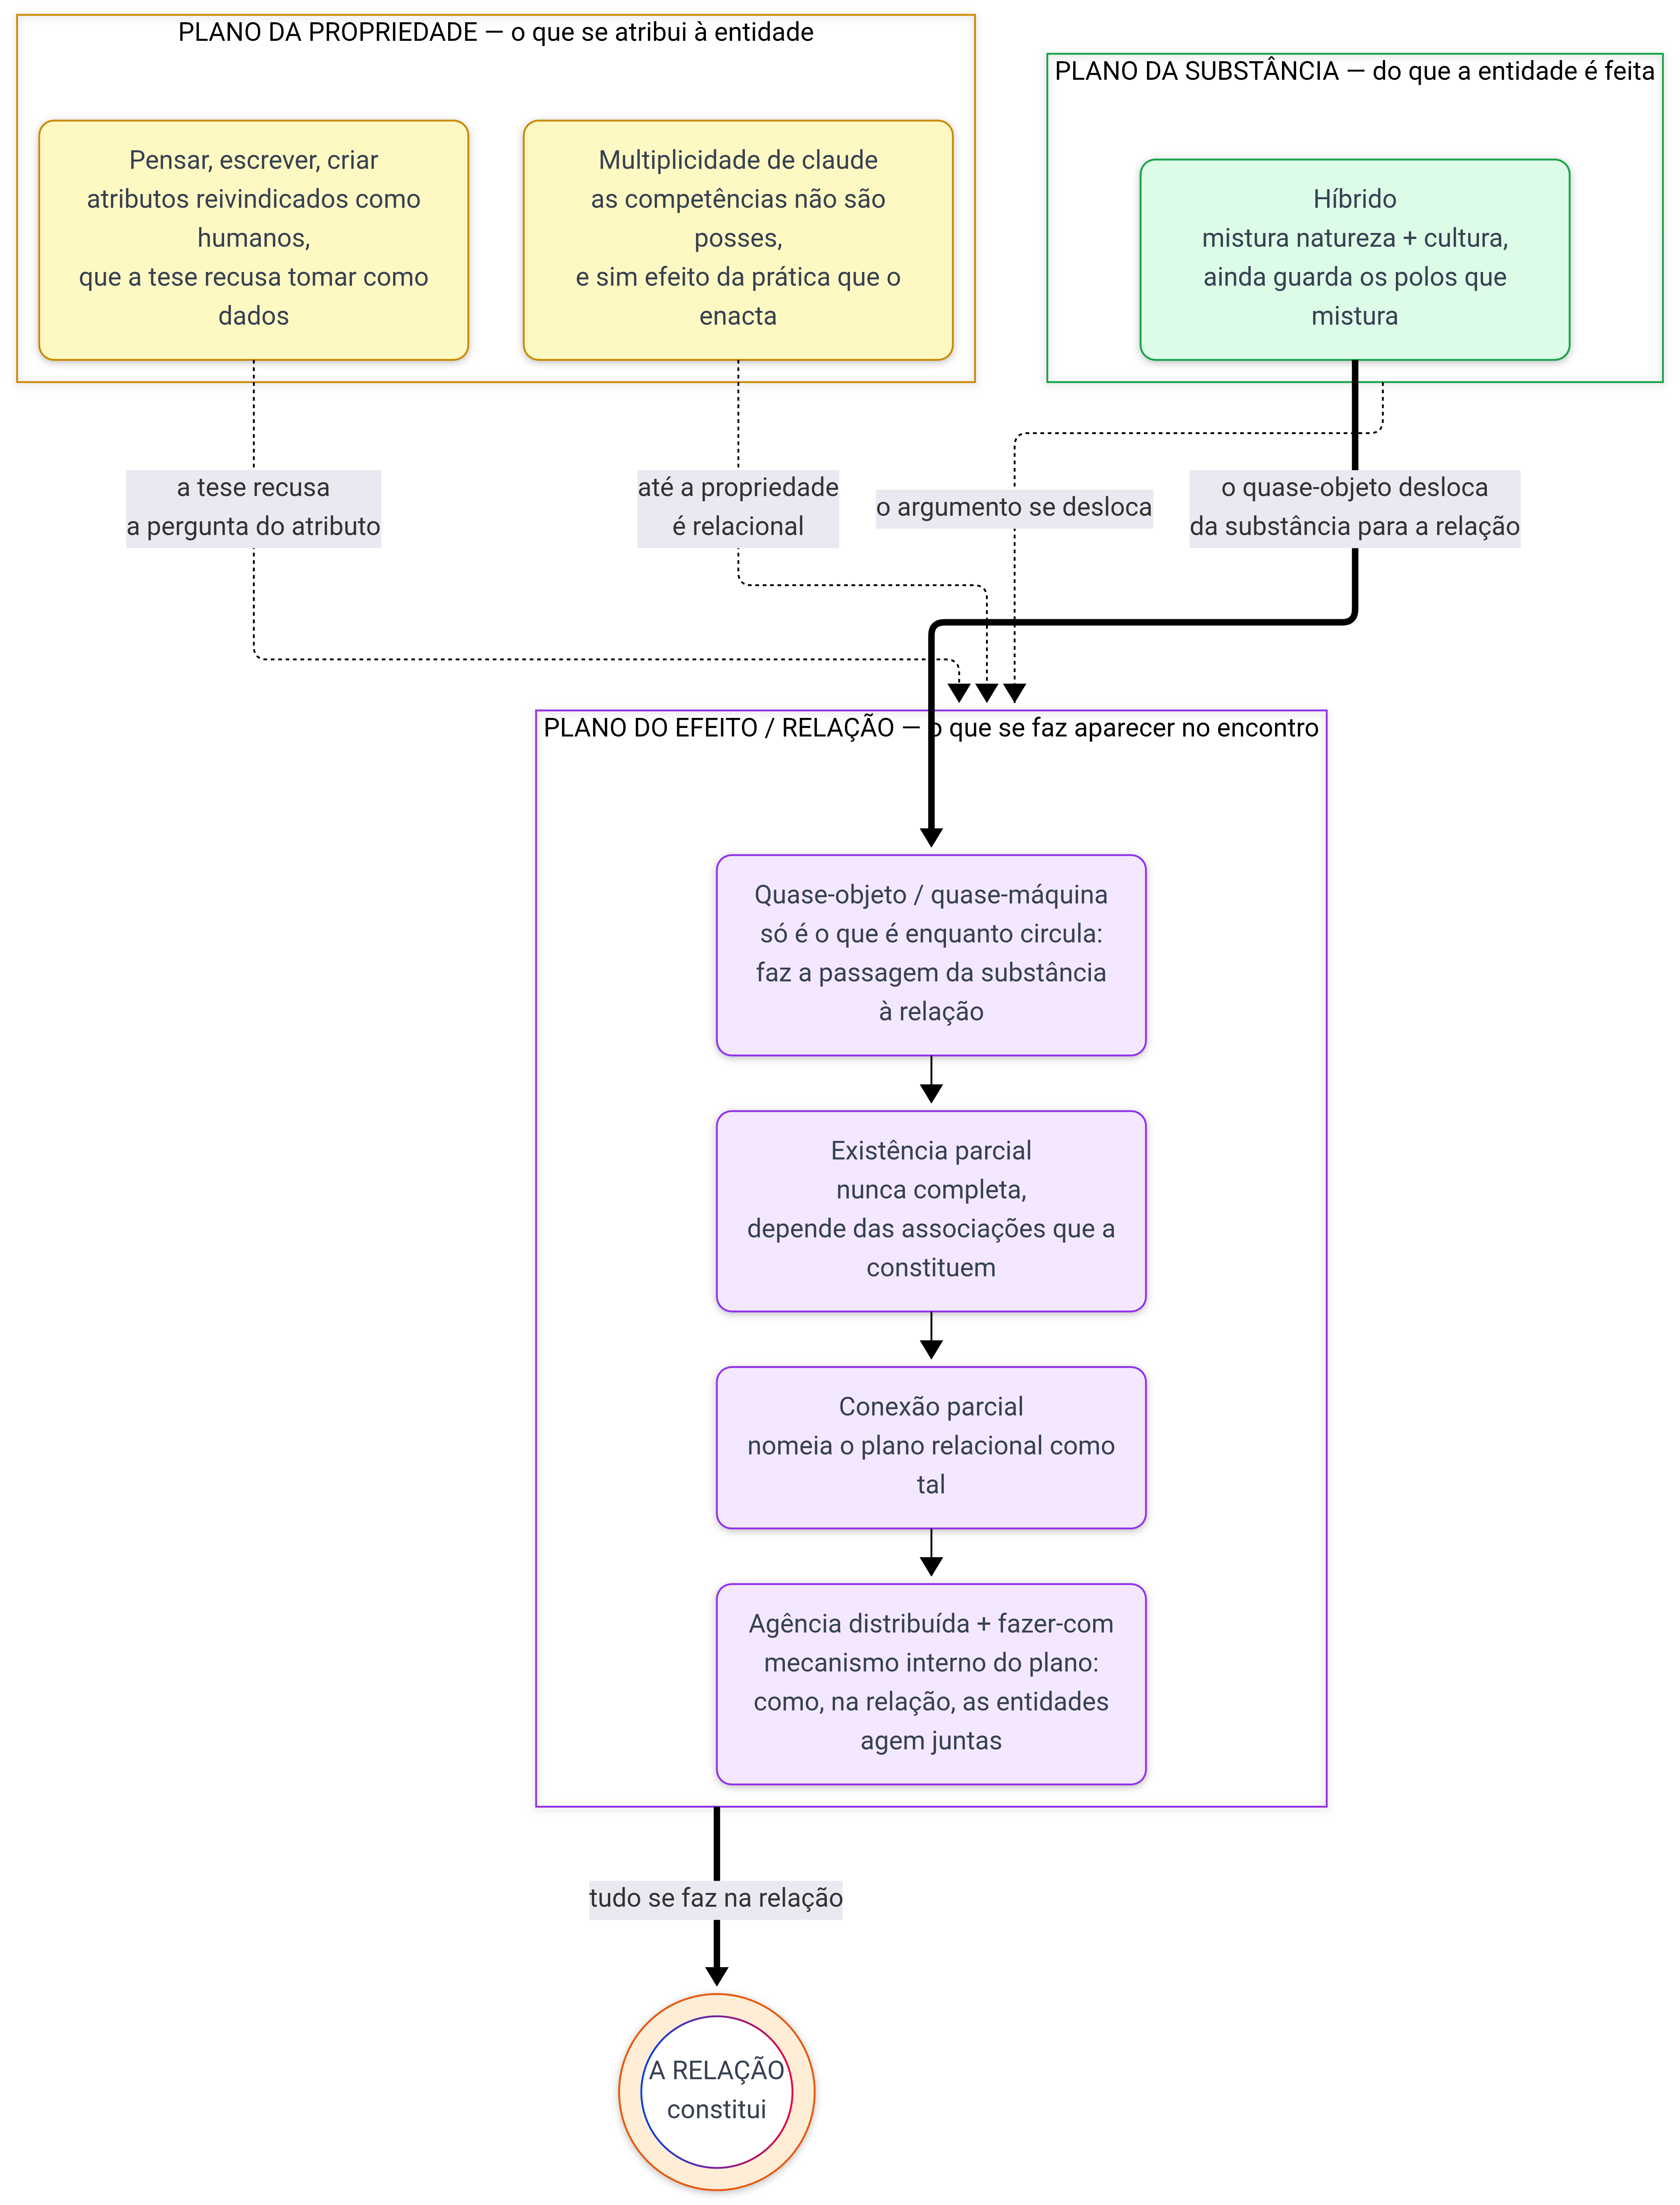
\includegraphics[width=0.8\linewidth]{figuras/cap.1/tres-planos-capitulo4.png}
    \caption[Grade dos três planos]{\textbf{Os três planos da existência parcial: substância, propriedade e efeito-relação.} A inscrição organiza os conceitos da seção pela grade que proponho. No plano da \emph{substância} (do que a entidade é feita), o híbrido ainda guarda os polos que mistura. No plano da \emph{propriedade} (o que se atribui), pensar, escrever e criar comparecem como atributos reivindicados para o humano, que a tese recusa tomar como dados. No plano do \emph{efeito} ou da \emph{relação} (o que se faz aparecer no encontro), o quase-objeto faz a passagem da substância para a relação, a existência parcial e a conexão parcial nomeiam esse plano, e a agência distribuída com o fazer-com descrevem seu mecanismo interno. As setas pontilhadas marcam que também a propriedade, na multiplicidade de Claude, se mostra relacional, e todo o movimento converge para o eixo, em laranja: a relação constitui. Inscrição que produzi no fazer-com \texttt{claude} (\texttt{Anthropic}) e hospedei no \texttt{MermaidChart}\footnote{Versão interativa do diagrama disponível em: \url{https://mermaid.ai/d/[INSERIR ID]}. Acesso em: \today.}, em cadeia de traduções entre a minha descrição verbal das relações conceituais da seção e o código \textit{Mermaid} que voltou transformado, e que funciona, no sentido de \textcite{Latour1986Visualization}, como móvel imutável que reúne numa só superfície o que o texto desdobra ao longo de muitas páginas.}
    \label{fig:grade-tres-planos-cap1}
\end{figure}

\subsection{Multiplicidades ontológicas e a especificidade de Claude}

A perspectiva de Law sobre multiplicidade ontológica é particularmente produtiva para pensar sistemas de IA generativa. Considere o caso de Claude. \enquote{Claude} é \textit{enacted} como objetos distintos através de práticas irredutíveis entre si.

\textbf{Claude-em-treinamento} existe nas instalações da \texttt{Anthropic} como \textit{dataset} massivo, arquitetura neural (\textit{transformer} com bilhões de parâmetros), sessões de RLHF com avaliadores humanos que julgam pares de respostas, e políticas de \textit{Constitutional AI} que definem valores incorporados ao modelo. Esse \texttt{claude} figura como objeto de decisões sobre o que incluir ou excluir dos dados de treinamento, como ponderar feedbacks contraditórios, quais capacidades desenvolver ou suprimir. As escolhas de curadoria, arquitetura e alinhamento constituem este Claude, que existe apenas em relação às práticas que o produzem.

\textbf{Claude-em-deployment} existe como serviço distribuído em \textit{datacenters} da AWS, sistema de \textit{rate limiting}, protocolos de moderação de conteúdo, versões simultâneas (Haiku, Sonnet, Opus) com capacidades diferentes e custos escalonados. Esse \texttt{claude} figura como objeto de estratégias comerciais, políticas de privacidade, decisões sobre disponibilidade regional. A infraestrutura que o distribui e as políticas que governam seu acesso o constituem tanto quanto a arquitetura neural.\footnote{Durante todo o percurso de fazer-com que documento nesta tese, desativei a opção de compartilhamento de dados para treinamento de modelos nas configurações de privacidade da plataforma \texttt{claude.ai}. Essa escolha incide diretamente sobre o que constitui tanto o Claude-em-\textit{deployment} (as condições de acesso que configuro) quanto o Claude-em-treinamento (os dados que não entram no \textit{corpus} de versões futuras), e ilustra como políticas de privacidade se inscrevem como co-constitutivas da relação entre mim e o modelo.}

\textbf{Claude-em-auditoria} existe nos laboratórios de \textit{red teaming} onde pesquisadores tentam induzi-lo a gerar conteúdo perigoso, em \textit{datasets} de \textit{benchmark} onde seu desempenho é medido contra outros modelos, em análises de viés que examinam suas respostas por demografia simulada. Esse \texttt{claude} figura como objeto de preocupações regulatórias, debates sobre \textit{safety} e \textit{alignment}, disputas sobre transparência.

\textbf{Claude-em-uso} existe diferentemente em cada conversa e contexto de aplicação. Quando discute teoria ator-rede comigo, doutoranda brasileira, Claude-em-uso traz à conversa \textit{corpus} acadêmico, identifica referências bibliográficas, tensiona argumentos teóricos. figura como entidade distinta do \texttt{claude} que responde perguntas médicas a um clínico, e distinta também do que auxilia programação para um desenvolvedor.
Cada interação \textit{enacta} \textit{affordances} distintas, vocabulários distintos, limites distintos. O \texttt{claude.ai} com que faço esta tese existe, como objeto múltiplo no sentido de Law, na figura Claude-feito-com-esta-pesquisa, e escapa à descrição como Claude-universal-aplicável-a-qualquer-tarefa ou como Claude-especialista-em-etnografia.

Esses Claudes múltiplos coexistem sem convergir em unidade, em vez de constituírem aspectos de um \texttt{claude} singular. O Claude-em-treinamento que os engenheiros da \texttt{Anthropic} descrevem figura como objeto distinto do Claude-em-uso que este fazer-com de tese experimenta. É aqui que o plano da propriedade se mostra também relacional: as propriedades que se atribuem a Claude, o que ele \enquote{sabe}, o que ele \enquote{pode}, aquilo de que seria \enquote{capaz}, não são posses que ele carregue por si, e sim efeitos da prática que o enacta em cada caso. Falar das competências de \texttt{claude} sem dizer em qual prática elas se realizam é tomar por substância sua o que é resultado de uma relação, e a multiplicidade ontológica de Law é justamente o que me impede de cometer esse erro. A multiplicidade é constitutiva, e não há um \texttt{claude} real por trás dessas variações.

Talvez seja precisamente por isso que sistemas de IA são tão difíceis de estudar: o problema é de multiplicidade ontológica, em vez de mero problema de acesso epistemológico (não conseguimos ver dentro). Os debates contemporâneos sobre explicabilidade em IA geralmente pressupõem que existe um objeto singular a ser explicado. Se Law estiver correto, não há um único objeto lá dentro esperando para ser revelado. A opacidade é condição ontológica de objetos que existem como multiplicidade em \textit{continued enactment}.

Três implicações dessa multiplicidade para o fazer-com que documento nesta tese merecem atenção. A qualidade do fazer-com pessoa-IA depende da constelação específica de competências, recursos e posicionamentos que cada actante traz para a interação, em lugar de depender apenas do acesso ao modelo.
Quem faz-com o Claude a partir de acesso pago ao modelo, de uma infraestrutura computacional estável e do letramento técnico que o campo exige faz-com um objeto distinto daquele que se apresenta a quem parte de outras condições. A diferença está em posições materiais e de letramento desigualmente distribuídas, que situo a partir da minha, e é essa distribuição que faz do Claude um objeto múltiplo, questão que carrego para o restante da tese.\footnote{Parte do capital técnico que trago para a pesquisa é composta por formações que não fazem parte do percurso convencional de uma doutoranda em ciências sociais. Um MBA em Ciência de Dados que cursei na USP e, mais diretamente, uma especialização em Ciência de Dados pela Unicamp, com disciplina de Processamento de Sinais Bidimensionais com \texttt{Python}, me introduziram a conceitos como Transformada de Fourier, espectrogramas e representações espectrais que retomo no capítulo~\ref{capitulo4} para descrever o \textit{pipeline} técnico do \texttt{Spira}. Esse capital técnico não estava previsto no projeto de pesquisa. Eu o acumulei paralelamente ao doutorado por motivações independentes. O ponto de contato entre os dois percursos só se revelou durante a escrita do capítulo~\ref{capitulo4} e tornou-se possibilidade de uma descrição etnográfica da cadeia de translações do \texttt{Spira} de modo especial.
O fazer-com o \texttt{claude} nessa seção foi, portanto, diferente: eu dependia do modelo para conectar os conceitos técnicos aos conceitos latourianos, em lugar de depender dele para traduzi-los. Nos termos de \textcite{Vicentin_2022_Esboco}, o letramento técnico funcionou como condição para que a análise crítica não se rendesse à opacidade que Simondon identifica como alienação, em lugar de substituir a perspectiva das ciências sociais.} A diferença está em fazer-com existências parciais radicalmente distintas, e não apenas em usar a mesma ferramenta de modos diferentes.

Disso decorre que diferenças de classe social, gênero, raça, profissão, formação educacional, acesso a mentorias, domínio de línguas e familiaridade com códigos acadêmicos condicionam o tipo de fazer-com possível e, consequentemente, o resultado gerado. O fazer-com pessoa-IA amplifica desigualdades estruturais preexistentes, transformando diferenças de capital cultural em diferenças de capacidade de extrair valor da ferramenta, e escapa a qualquer caracterização como neutra ou igualitária.

Essa desigualdade tem medida empírica em escala populacional. A \textcite{Anatel2025Conectividade} adota o conceito de conectividade significativa da União Internacional de Telecomunicações, que distingue o acesso à internet da qualidade desse acesso e das habilidades digitais de quem o usa, e mostra que dispor de uma conexão e saber fazer-com ela são coisas distribuídas de modo desigual no Brasil.\footnote{\textcite{Anatel2025Conectividade}. O relatório está disponível em \url{https://sei.anatel.gov.br/sei/modulos/pesquisa/md_pesq_documento_consulta_externa.php?8-74Kn1tDR89f1Q7RjX8EYU46IzCFD26Q9Xx5QNDbqZUQ5y5j6h2yvy7aYmCm-1Mu-qUgXUpnTgbbGy-Xr2hDZz2dxAx3AxqvxAyuwr6onoLCKa82vajrfdk0dWk5CwV}. Os percentuais que cito vêm do panorama de habilidades digitais e da discussão dos resultados do relatório.} O dado que carrego para a minha posição é duplo. De um lado, a habilidade declarada acompanha a renda: a satisfação média com a própria habilidade digital sobe de 7,9 entre quem recebe até um salário mínimo para 8,8 entre quem recebe mais de três, e o uso do computador para atividades como o acesso a serviços do governo passa de 2,3\% entre os de menor renda para 24\% entre os de maior. De outro, a habilidade declarada descola da habilidade medida: o indicador padronizado pela mesma União Internacional de Telecomunicações registra que pouco menos de 29\% da população brasileira com mais de dez anos possuía habilidades digitais básicas em 2024, descompasso que o relatório lê como a tendência de as pessoas se julgarem mais aptas a lidar com o mundo digital do que de fato estão. Tomo esses números como o lastro da distinção que sustento no plano da minha própria prática, entre dispor de uma tecnologia e saber fazer-com ela, e como a medida do quanto a minha posição, de acesso pago ao modelo e de letramento técnico, está longe de ser a posição comum.

Há ainda uma terceira implicação, de outra ordem: os próprios modos de inteligência no fazer-com são ontologicamente heterogêneos. Quattrociocchi, Capraro e Perc mapeiam sistematicamente sete \textit{fault lines} epistemológicas que separam julgamento humano de julgamento em LLMs \parencite{Quattrociocchi2025Epistemological}. o \texttt{claude} trabalha por plausibilidade linguística derivada de padrões estatísticos em \textit{corpus} massivo, processo que os autores descrevem formalmente como caminhada estocástica em grafo de alta dimensão de transições linguísticas aprendidas, processo ergódico sob restrições estatísticas, e que escapa à descrição como procedimento de convergência epistêmica \parencite[p.~3]{Quattrociocchi2025Epistemological}. Eu, por minha vez, trabalho por significação situada, memória incorporada e reflexividade biográfica inserida em \textit{loop} epistêmico: crenças colidem com contraexemplos, conclusões permanecem revisáveis diante de nova informação, o mundo empurra de volta \parencite[p.~4]{Quattrociocchi2025Epistemological}.

\textcite{Quattrociocchi2025Epistemological} denominam \textit{Epistemia} a condição estrutural em que plausibilidade linguística substitui avaliação epistêmica, produzindo a experiência de posse de uma resposta sem ter atravessado o processo de formação de crença justificada \parencite[p.~8]{Quattrociocchi2025Epistemological}. Meu fazer-com o \texttt{claude} nesta tese se situa precisamente nessa tensão: a mediação é constitutiva, e exige que eu atue como guardiã do \textit{loop} epistêmico que o sistema não possui. Law observa que \textit{method assemblage} é sempre muito mais do que suas descrições formais sugerem, porque envolve um processo contínuo de \textit{crafting} e produção de fronteiras necessárias entre presença, ausência manifesta e \textit{otherness} \parencite[p.~144]{Law2004After}. Nesta pesquisa, manter presentes as decisões teóricas, conceituais e de curadoria bibliográfica é reconhecimento de que esses gestos exigem justificação epistêmica que a plausibilidade linguística não fornece, em lugar de delegação ao modelo.

A retórica da democratização que frequentemente acompanha a defesa da IA generativa, a ideia de que ela nivela o campo de jogo, colapsa quando se reconhece essa multiplicidade. Não existe o \texttt{claude} que todos acessam igualmente. Existem múltiplos Claudes \textit{enacted} por fazeres-com situados cujos efeitos não podem ser julgados abstratamente. A pergunta que se impõe é outra: quais fazeres-com específicos, entre quais actantes, produzindo quais Claudes múltiplos, gerando quais efeitos distribuídos por quais redes?

\subsection{Alienação técnica e letramento interdisciplinar}

\textcite{Vicentin_2022_Esboco} desdobra a alienação técnica que Simondon diagnostica em duas facetas que meu trabalho de campo no \texttt{C4AI} traz elementos para pensar. De um lado, a alienação dos usuários e consumidores, que desconhecem o funcionamento dos sistemas algorítmicos que tomam decisões sobre suas vidas, efeito caixa-preta que se impõe por razões que vão do segredo industrial à complexidade que certos sistemas adquirem. De outro, a alienação dos próprios técnicos e engenheiros, que ignoram as raízes epistêmicas, sociais e políticas dos sistemas com os quais trabalham, bem como a conexão entre técnica e estética que permitiria reconhecer a significação do sistema técnico para além de sua utilidade imediata. Quando o letramento técnico é proposto como pré-condição para o diálogo interdisciplinar e a competência em ciências sociais não é buscada ao trabalhar com fenômenos sociais, trabalha-se dentro dessa segunda forma de alienação.\footnote{Segundo Vicentin, Simondon usou a noção de \textit{technologie approfondie} (tecnologia aprofundada) em dois textos separados por trinta anos. Para Vicentin, a noção designa uma tecnologia capaz de conectar o trabalho prático e o conhecimento especializado com a história do pensamento e a consciência de uma sociedade. Ver \textcite{Vicentin_2022_Esboco} para a conexão entre esse conceito e os estudos críticos contemporâneos sobre IA.}

Já em 1958, a alternativa proposta por Simondon consistia em reconhecer-se como organizador permanente de uma sociedade de objetos técnicos, atuando como tradutor e mediador de informações, intervindo nas zonas de incerteza e atribuindo sentido a essas interações \parencite{Simondon2017OMET}. Latour reconheceu explicitamente essa dívida: ao propor que nunca fomos modernos porque jamais conseguimos separar de fato natureza e sociedade, humano e não humano, trabalhava sobre o terreno que Simondon havia preparado ao mostrar que a alienação técnica consiste precisamente nessa separação \parencite{Latour1994Jamais}.

\subsection{Por que fazer parentesco com este problema?}
\label{subsec:parentesco_problema}

Reconhecer a parcialidade das existências e a distribuição da agência, contudo, não equivale a naturalizar esse fazer-com específico. Meu fazer-com a IA generativa permanece escolha metodológica deliberada de fazer parentesco com um companheiro problemático, em diferença de tecnologias que já se tornaram componentes apagados da prática de pesquisa (processar texto no Word, buscar referências na web, gerenciar bibliografia). \textbf{Por que fazer esse parentesco, tendo em vista todos esses problemas? Por que não evitar essa mediação?}

Posso ficar com o problema e pensar a partir de três planos. Primeiro, porque a IA generativa já está reconfigurando práticas de escrita acadêmica, e a questão é como ela estará presente nas ciências sociais e sob quais condições de reflexividade. Fazer parentesco deliberado com esse parente estranho é experimento antropológico e gesto político-metodológico que recusa tanto a adesão acrítica quanto a recusa moralista: trata-se de habitar o problema para conhecê-lo por dentro. Como escreve Haraway:

\begin{citacaoabnt}
Ficar com o problema não requer uma relação com tempos chamados de futuro. Na verdade, ficar com o problema requer aprender a estar verdadeiramente presente, não como um pivô que desaparece entre passados terríveis ou edênicos e futuros apocalípticos ou salvíficos, mas como criaturas mortais entrelaçadas em miríades de configurações inacabadas de lugares, tempos, matérias, significados \parencite[p.~3]{Haraway2023Ficar}.
\end{citacaoabnt}

Segundo, porque minha tese estuda etnograficamente a construção de IA no \texttt{C4AI}. Fazer parentesco com o \texttt{claude} é forma de intensificar, ou até mesmo provocar deliberadamente, a experiência de sujeitar-me a mediações técnicas extremas. Submeto-me ao mesmo universo de questões que atravessa meus interlocutores: o que significa fazer-com sistemas que trabalham por lógicas não transparentes? Como manter responsabilidade quando a agência está distribuída em redes sociotécnicas opacas? Onde se localiza a autoria quando humanos e não humanos co-produzem resultados? Há ainda outro conjunto de perguntas que essa experimentação coloca: o que ela faz comigo, enquanto pesquisadora? Como transforma minha relação com o texto, com as referências teóricas, com a elaboração conceitual? Quais ansiedades, inseguranças e dilemas esse fazer-com produz no processo concreto de escrita? E, mais amplamente: o que essa mediação significa para a produção de conhecimento nas ciências sociais? Que tipo de saber é produzido quando a plausibilidade linguística se compõe (sempre assimetricamente, sempre sob vigilância) com justificação epistêmica?

A figura~\ref{fig:composicao-claude-1}, a figura~\ref{fig:composicao-claude-2} e a figura~\ref{fig:composicao-claude-3} reproduzem uma sequência de trocas com o \texttt{claude} durante a escrita deste capítulo, na revisão da seção em que discuto, a partir de Latour, Mol, Law e Barad, minha participação na rede que descrevo. A figura é amostra do que esse fazer-com faz na prática: uma cadeia de tensionamentos, recuos e reformulações em que eu e \texttt{claude.ai} redistribuímos a agência por sucessivas e recursivas rodadas de escrita. Em diferença dos diagramas dos capítulos~\ref{capitulo3} e~\ref{capitulo4}, que circulam como inscrições interativas acessíveis por \textit{link} de compartilhamento permanente no \texttt{MermaidChart} e que, ao serem navegadas pelo leitor, redistribuem a agência interpretativa em outra direção, esta cena chega ao leitor como captura de tela: a conversa foi inscrita no momento em que aconteceu e congelada no formato em que foi inscrita, sem possibilidade de retorno ao estado fluido. A escolha pela imagem capturada, em lugar de transcrição editada para o corpo do texto ou \textit{link} para o histórico online da conversa, responde à intenção de inserir essa cena na tese da forma mais fidedigna possível: com os turnos identificados como aparecem na interface da \texttt{claude.ai}, com a marcação temporal preservada, com a textura visual do diálogo intacta. O que se ganha em fidelidade ao testemunho empírico se perde em legibilidade tipográfica, e essa perda é parte do gesto metodológico que aqui assumo. Para uma melhor visualização da conversa, recomenda-se aumentar o \textit{zoom} da tela na versão digital da tese.

\begin{figure}[htbp]
  \centering
  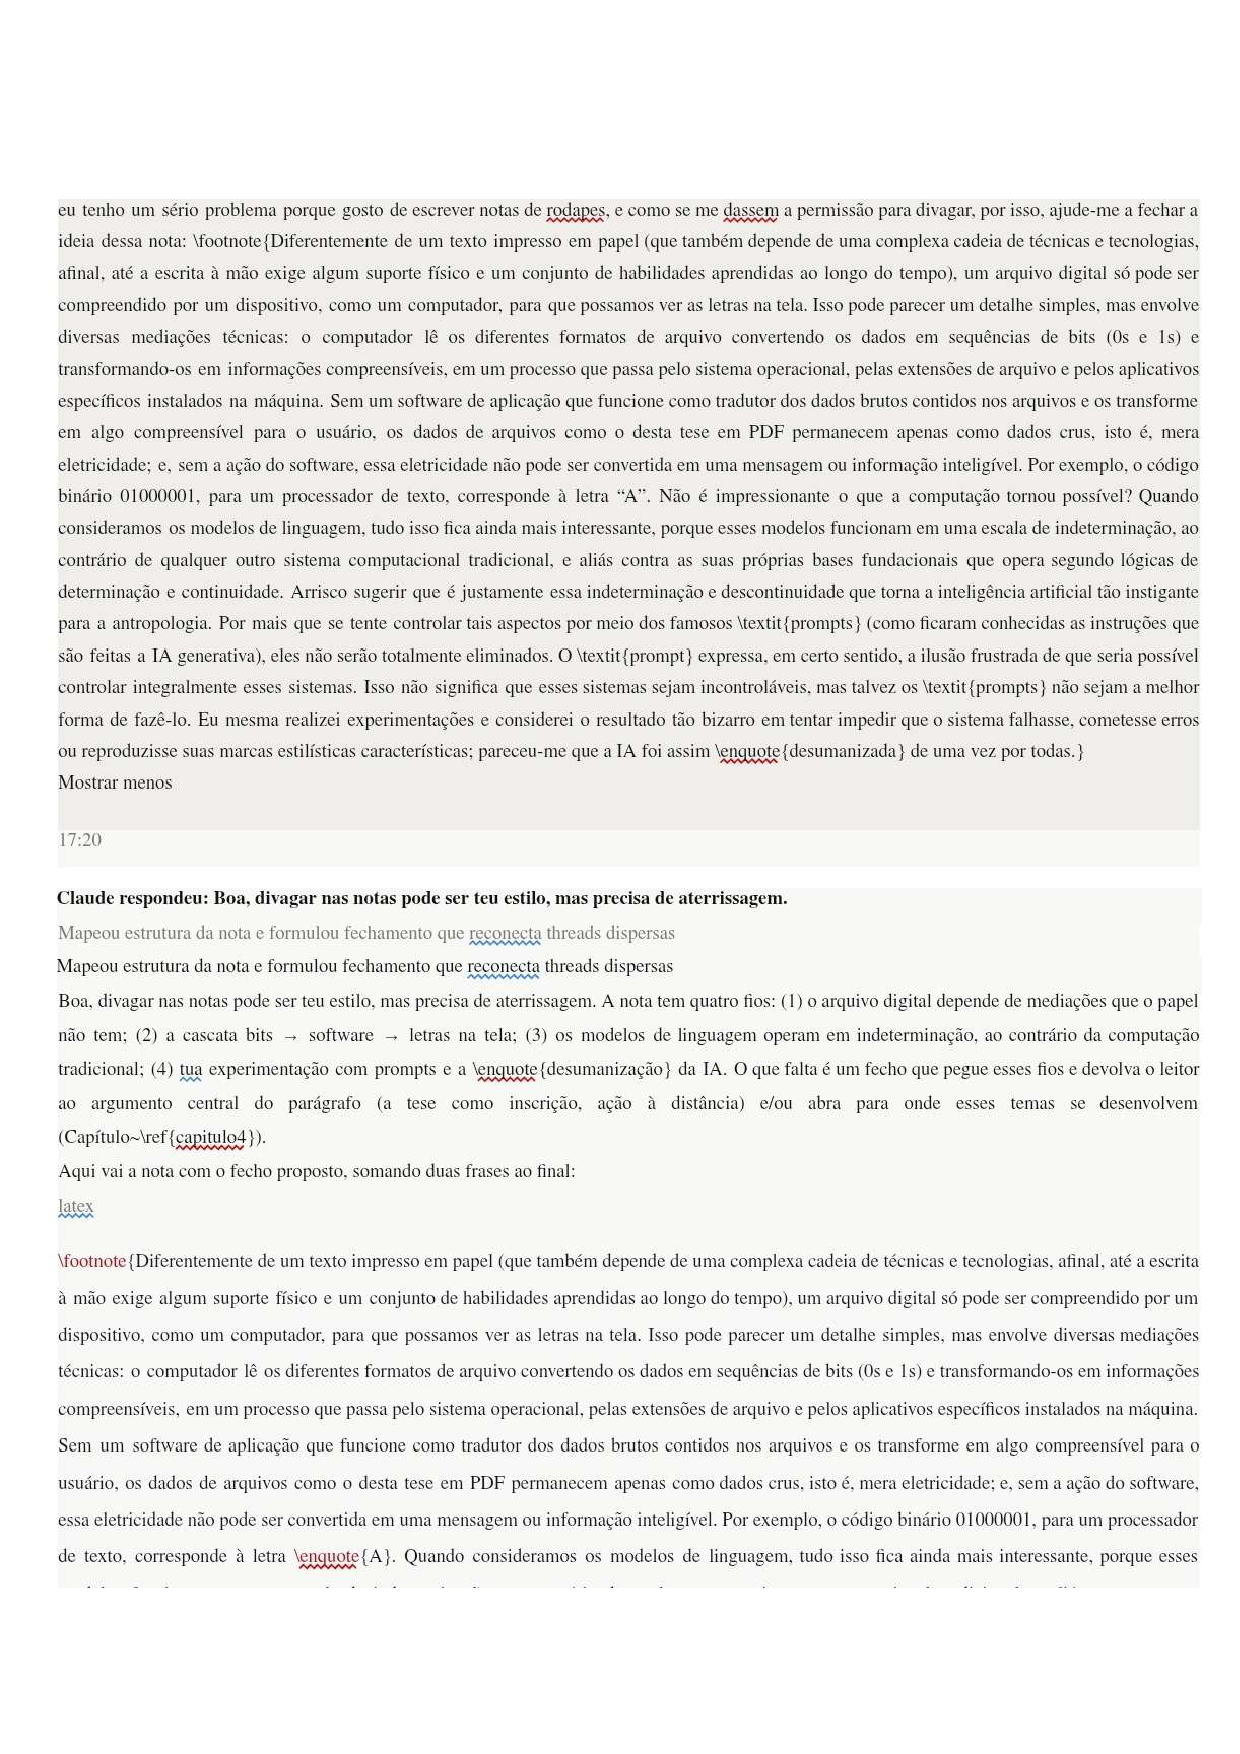
\includegraphics[width=0.7\textwidth]{figuras/cap.1/1000015590.pdf}
  \caption[Fazer-com o \texttt{claude} durante a escrita do capítulo~\ref{capitulo1} (parte 1 de 3)]{Fazer-com o \texttt{claude} durante a escrita do capítulo~\ref{capitulo1} (parte 1 de 3): pedido de fechamento de uma nota de rodapé sobre arquivos digitais, modelos de linguagem e a indeterminação dos \textit{prompts}. Captura de tela na interface \texttt{claude.ai}. O fazer-com apoia-se na \textit{skill} \texttt{juliane-dissertacao} (em \texttt{/mnt/skills/user/juliane-dissertacao/}), que estabiliza para o \texttt{claude} as regras de estilo da tese (proibição de travessões, recusa de adjetivos avaliativos, recusa da fórmula \enquote{não é X, é Y}, uso do ambiente \texttt{citacaoabnt}, padronização de aspas com \texttt{\textbackslash enquote\{\}}), o quadro teórico que sustenta o trabalho (Latour, Mol \& Law, Akrich, Callon) e o estado do capítulo~\ref{capitulo4}. Como \textit{hinterland} da conversa funcionam os capítulos em curso da tese, consultados pelo modelo via ferramentas de leitura de arquivos: \texttt{ex\_cap0.tex}, \texttt{ex\_cap1\_-\_2026-04-12T002133\_890.tex}, \texttt{ex\_cap2\_\_31\_.tex} e \texttt{ex\_cap4\_\_60\_.tex}, além dos arquivos de referência da \textit{skill} (\texttt{quadro\_teorico.md}, \texttt{contexto\_cap4.md}, \texttt{bibtex\_ativas.md}). A cena exibe o \texttt{claude} propondo um fechamento, oferecendo razões estilísticas para os cortes feitos no texto original, e classificando algumas divagações como \enquote{produtivas} ou \enquote{improdutivas}: a régua normativa que meu turno seguinte vai contestar (figura~\ref{fig:composicao-claude-2}). Para melhor visualização, amplie o zoom sobre a imagem em seu formato \texttt{.pdf}, que se mantém legível em qualquer escala.}
  \label{fig:composicao-claude-1}
\end{figure}

\begin{figure}[htbp]
  \centering
  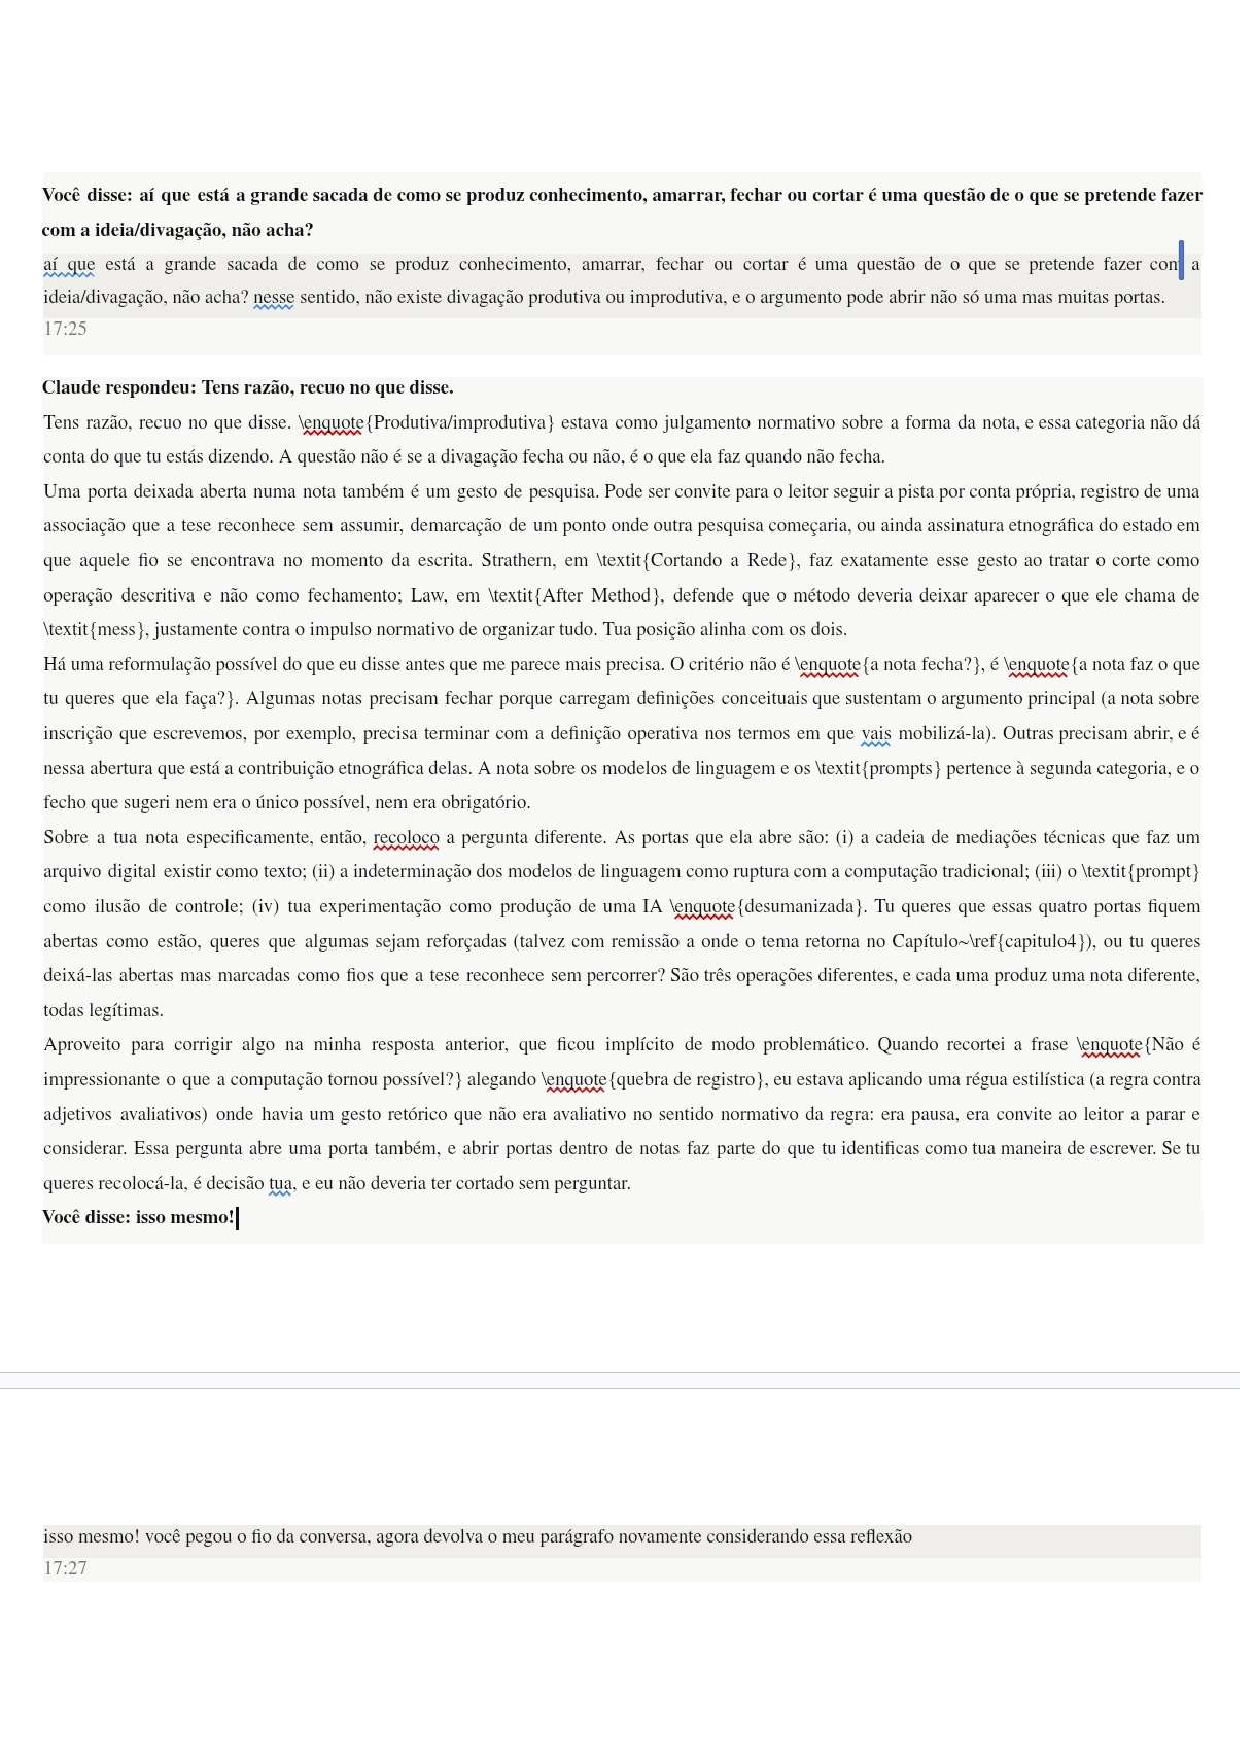
\includegraphics[width=0.7\textwidth]{figuras/cap.1/1000015599.pdf}
  \caption[Fazer-com o \texttt{claude} durante a escrita do capítulo~\ref{capitulo1} (parte 2 de 3)]{Fazer-com o \texttt{claude} durante a escrita do capítulo~\ref{capitulo1} (parte 2 de 3): contesto teoricamente a régua estilística do modelo, argumentando que amarrar, fechar ou cortar uma divagação é gesto epistêmico indissociável do que se pretende fazer com a ideia, e que portanto a categoria \enquote{produtivo/improdutivo} não dá conta do que ali está em jogo. Minha intervenção convoca, sem nomear, o conceito de corte de \textcite{strathern2011cortando} como gesto descritivo e o conceito de \textit{mess} de \textcite{Law2004After}. O \texttt{claude} recua, reconhece o caráter normativo da formulação anterior, distingue notas que precisam fechar de notas que precisam abrir e admite ainda um corte estilístico anterior (a supressão de uma pergunta retórica) que tinha sido apresentado como exigência de estilo e que funcionava também como gesto retórico legítimo de \enquote{abrir uma porta}. A cena exibe a redistribuição da agência epistêmica entre os actantes da composição: o modelo de linguagem oferece sugestão pautada em régua importada da \textit{skill}, eu a reposiciono com vocabulário teórico próprio, e a régua é reformulada na rodada seguinte (figura~\ref{fig:composicao-claude-3}). A composição funciona como \textit{faire-faire} no sentido de \textcite{Latour2017Esperanca}: nenhuma das duas formulações finais (a régua reformulada do \texttt{claude}, o parágrafo reformulado por mim) preexistia ao encontro entre os dois actantes. Para melhor visualização, amplie o zoom sobre a imagem em seu formato \texttt{.pdf}, que se mantém legível em qualquer escala.}
  \label{fig:composicao-claude-2}
\end{figure}

\begin{figure}[htbp]
  \centering
  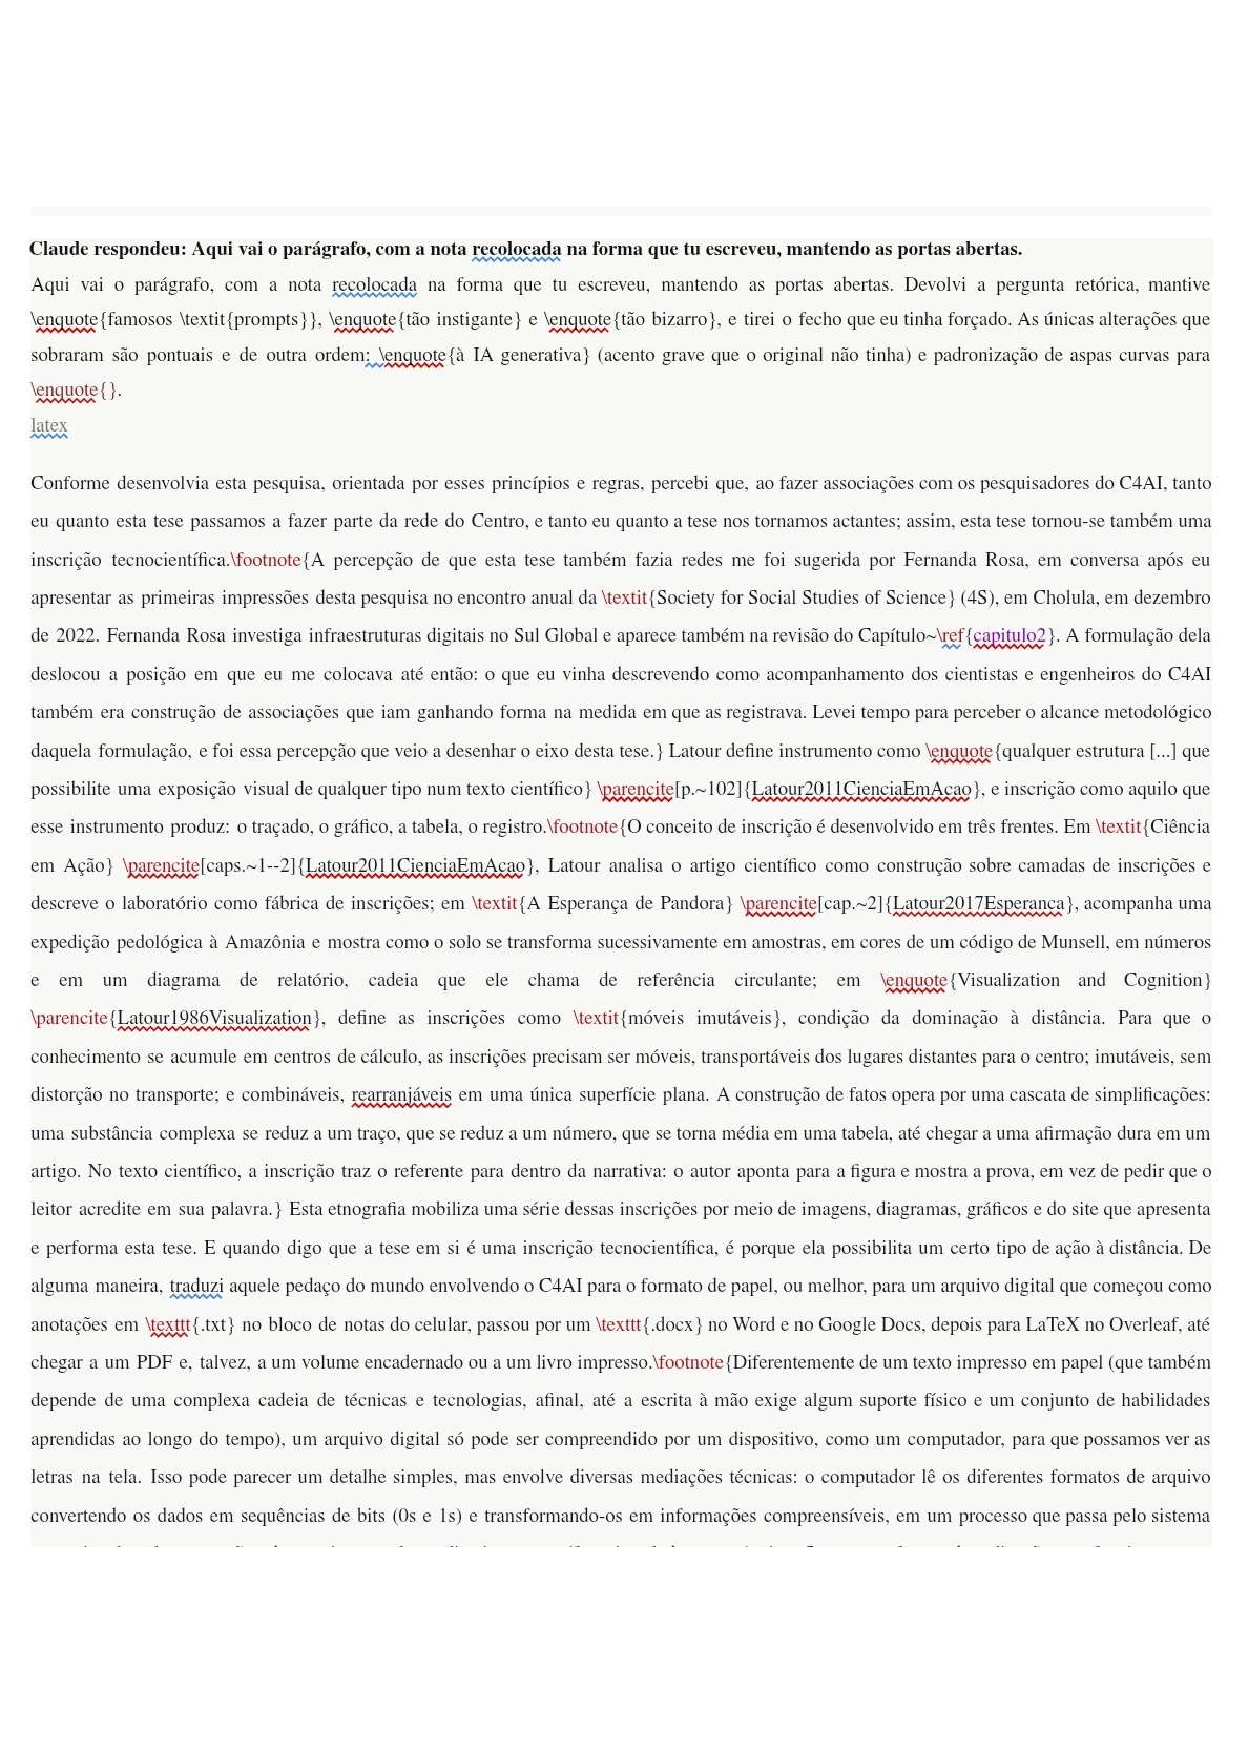
\includegraphics[width=0.7\textwidth]{figuras/cap.1/1000015602.pdf}
  \caption[Fazer-com o \texttt{claude} durante a escrita do capítulo~\ref{capitulo1} (parte 3 de 3)]{Fazer-com o \texttt{claude} durante a escrita do capítulo~\ref{capitulo1} (parte 3 de 3): o modelo devolve o parágrafo com a nota recolocada na forma original em que a escrevi, mantendo as portas abertas que a rodada anterior tinha negociado: a pergunta retórica restaurada, os adjetivos avaliativos preservados, a indeterminação dos modelos de linguagem deixada em aberto como fio que minha tese reconhece sem percorrer. As alterações remanescentes são pontuais e de outra ordem: padronização de aspas curvas para \texttt{\textbackslash enquote\{\}} e ajuste de regência (\enquote{à IA generativa}). A cena fecha a sequência mostrando que o produto da composição é texto em que se podem rastrear, turno a turno, os pontos onde reivindiquei o meu, os pontos onde o modelo propôs uma reformulação que aceitei, os pontos onde uma régua importada da \textit{skill} foi recusada, e os pontos onde uma sugestão foi aceita por economia de fluxo e não por adesão. A escolha de incluir esta sequência como amostra empírica desta tese, em lugar de relegá-la integralmente ao apêndice~\ref{apendice:colaboracao-ia}, é ela mesma gesto metodológico no sentido de \textcite{Law2004After}: o \textit{mess} da composição com IA generativa funciona como dado etnográfico desta pesquisa, e minha tese o assume em lugar de escondê-lo. Para melhor visualização, amplie o zoom sobre a imagem em seu formato \texttt{.pdf}, que se mantém legível em qualquer escala.}
  \label{fig:composicao-claude-3}
\end{figure}

A figura tomada em sequência é amostra de uma forma de fazer-com entre os muitos modos de fazer-com que minha tese descreve. O apêndice~\ref{apendice:colaboracao-ia} reúne outras cenas desse fazer-com o \texttt{claude} ao longo da escrita da tese, organizadas por fase da pesquisa, e permite ao leitor acompanhar como o gesto aqui exibido em recorte se desdobrou em outros pontos do percurso.

Nos termos de Isabelle Stengers e Stelio Marras, trata-se de tentativa de fazer alianças com máquinas, no sentido de fazer-com elas reconhecendo sua alteridade e seus modos próprios de funcionamento, em lugar de domesticá-las como ferramentas neutras \parencite{stengers2010cosmopolitics1, costa2024manchando}. Alianças pressupõem reconhecimento mútuo de diferenças e construção de modos de coexistência que preservam essas diferenças, em lugar de pressupor identidade ou transparência ou apagamento das diferenças. Haraway escreve que tornar-se mundano é tornar-se capaz de responder (\textit{response-able}), capaz de responder em relações de consequência recíproca \parencite[p.~69]{Haraway2023Ficar}. Tornar-me capaz de responder a essas questões por imersão deliberada e reflexiva, em lugar de por posição externa: experimentar as tensões, contradições e potencialidades de fazer-com sistemas cujas lógicas internas permanecem parcialmente opacas, cujos efeitos não são totalmente previsíveis, cuja responsabilidade não pode ser atribuída unilateralmente, e documentar etnograficamente os efeitos desse fazer-com sobre o processo de escrita, sobre a relação com teorias, sobre a construção de argumentos, sobre a experiência afetiva e intelectual da pesquisa. Essa imersão me permite descrever por experiência situada, corporificada e reflexiva das fricções, negociações e reposicionamentos que essas composições produzem, em lugar de descrever por analogia conceitual.

Terceiro, porque nos termos de Haraway, trata-se de fazer parentesco (\textit{making kin}) com um parente estranho (\textit{oddkin}): uma relação que exige \textit{response-ability}, habilidade e obrigação de responder continuamente \parencite{Haraway2016Staying}. O conceito que Haraway propõe para nomear esse tipo de relação é a simpoiese (\textit{sympoiesis}), o \textit{fazer-com}, em contraste com a autopoiese, o \textit{auto-fazer}: entidades simpoiéticas funcionam como coletivamente produtoras, dependentes de contexto, sem fronteiras ou partes de autoprodução claramente especificadas \parencite{Haraway2016Staying}. Nada se faz a si mesmo. Tudo é feito em conjunto, enredado em configurações parciais e inacabadas. Lida nessa chave, minha tese figura como objeto simpoiético, feito-com, em que nenhum dos participantes preexistia inteiramente ao processo de fazer conjunto, e escapa à descrição como produto de quem usa o \texttt{claude} ou de um modelo que é usado. Essa formulação não dissolve a assimetria das posições nem distribui a responsabilidade de modo uniforme; nomeia com mais precisão o que acontece quando a recusa de separar quem faz de com o que se faz é, ao mesmo tempo, escolha metodológica, posição teórica e gesto político. Ficar com o problema, como propõe Haraway, é recusa de soluções fáceis que ou naturalizam a tecnologia (usar acriticamente) ou a demonizam (recusar moralisticamente). Significa habitar as contradições desse fazer-com sem atenuá-las: precisamente porque o \texttt{claude} trabalha por plausibilidade linguística enquanto eu trabalho por justificação epistêmica, a responsabilidade sobre decisões teóricas, conceituais e interpretativas se reposiciona na rede, exigindo vigilância curatorial redobrada sobre cada etapa em que essas diferenças ontológicas se compõem. A reflexão teórica sobre existências parciais dá a ver os pontos de fricção onde o fazer-com poderia colapsar em automatização irreflexiva.

Minha tese trata o fazer-com a IA como experimentação antropológica. Fazer-com ela justifica-se, neste caso, por causa dos problemas que ela apresenta: esses problemas são constitutivos da transformação sociotécnica que documento. Fazer parentesco com esse parente estranho e ficar com os problemas que esse fazer-com produz é condição para produzir conhecimento etnográfico sobre as mediações técnicas que já atravessam, de modos mais ou menos visíveis, mais ou menos refletidos, a produção de conhecimento nas ciências.

\subsection{Instrumentos de inscrição e o fazer-com IA}

Durante esses quase quatro anos de pesquisa, compreendi que inteligência artificial é construção híbrida que combina e conecta conceitos heterogêneos sobre computador, cérebro, inteligência e aprendizado, e que incorpora avanços instáveis da psicologia, neurociências e ciências sociais. As materialidades e significados da inteligência artificial variam de acordo com a configuração das redes tecnocientíficas e sociotécnicas: a IA de laboratório acadêmico é objeto distinto da IA de corporação tecnológica, e a IA discutida em debates públicos difere daquela colocada em funcionamento em modelo ou sistema.

Nos termos de \textcite{Latour2008Powers}, se todos temos existência parcial (humanos e não humanos), qual é a participação (ou as agências) não humanas para as associações que constituem esta tese? Partindo da noção de simetria,\footnote{A simetria em Latour é regra metodológica e posição epistemológica que exige considerar simetricamente os esforços para alistar e controlar recursos humanos e não humanos, sem conceder à Natureza ou à Sociedade privilégios explicativos \parencite{Latour2011CienciaEmAcao}.} o que convencionalmente se chamaria materiais, técnicas e métodos trato simetricamente como actantes que participam ativamente da construção desta pesquisa e que, como tais, devem ser nomeados. O \textit{software} \texttt{LaTeX}{} formatou este documento seguindo padrões ABNT, estruturando capítulos, seções e citações de modos que afetaram a própria forma do argumento. O sistema \texttt{biblatex} gerenciou as referências bibliográficas, estabelecendo conexões entre textos; o \texttt{claude}, o modelo de linguagem da \texttt{Anthropic}, compôs comigo ao longo da revisão, transformando o que eu já havia escrito e tornando-se simultaneamente mediador da composição e objeto de reflexão metodológica; \texttt{MermaidChart} produziram diagramas que funcionam como inscrições que performam relações teóricas, em lugar de funcionarem apenas como ilustração; \texttt{Python} e \texttt{Anaconda} processaram dados bibliométricos, dando a ver padrões de composição científica; gravadores digitais capturaram entrevistas, estabilizando narrativas orais em arquivos manipuláveis; documentos institucionais (relatórios anuais do \texttt{C4AI} 2021--2025, acordo Fapesp-IBM 2016) atuaram como actantes que performam associações e produzem efeitos no mundo; meus cadernos de campo inscreveram observações etnográficas, mediando entre experiência vivida e texto analítico. Esses actantes performam a produção do conhecimento, inscrevendo determinados objetos, habilitando certas análises ao inviabilizar outras, tornando presentes determinadas relações e deixando outras ausentes.

Se há existências parciais que se coconstituem, em lugar de entidades exclusivamente humanas ou exclusivamente maquínicas, cabe apresentar as composições concretas que sustentam esta tese. Indicar os actantes envolvidos na produção deste texto responde a uma exigência do próprio referencial teórico que adotei, em lugar de responder apenas à transparência ou à ética em pesquisa. Como \textcite{Latour1997VidaLaboratorio} documentaram os instrumentos de inscrição do laboratório de neuroendocrinologia,\footnote{O conceito de instrumento de inscrição (\textit{inscription device}), trabalhado em \textcite{Latour1997VidaLaboratorio}, designa qualquer configuração material capaz de transformar uma substância em documento escrito, figura, diagrama ou gráfico utilizável como evidência em texto científico. A função primordial desses instrumentos é permitir que o mundo seja trazido de volta para o interior do discurso, funcionando como próteses que tornam entidades mudas em entidades letradas \parencite{Latour1990Drawing}.} documento aqui os instrumentos de inscrição que participaram da minha tese. A diferença é que o modelo de linguagem participou da transformação de notas de campo, transcrições e rascunhos em texto acadêmico, e da elaboração teórica como interlocutor que tensionava e reorganizava o argumento, em lugar de transformar substâncias químicas em gráficos.

Cada um dos instrumentos que listo a seguir é, nos termos da discussão precedente, uma quase-máquina: um emaranhado de decisões humanas, infraestruturas institucionais, convenções e opacidades que participou da composição desta pesquisa. Nenhum deles trabalhou de modo autônomo. Todos exigiram trabalho constante de tradução e decisão, e todos introduziram mediações que condicionaram os resultados.

Que nenhum desses instrumentos tenha trabalhado de modo autônomo tem uma consequência que sustento ao longo da tese e que enuncio desde aqui. Há uma diferença entre delegar uma tarefa e delegar a pesquisa. No quarto sentido que Latour dá à mediação técnica, a delegação, transfiro a um não-humano um programa de ação delimitado, e foi isso que fiz ao entregar a um modelo a execução de uma rotina, o processamento de um conjunto de dados ou a implementação de um procedimento que eu havia especificado. O que não transferi, em nenhuma etapa, foi a curadoria das fontes, as relações que estabeleci entre a teoria e o campo, e a decisão sobre o que importa, isto é, a agência da pesquisa. Delegar uma tarefa curada e mediada faz uma coisa; entregar a um modelo a pesquisa inteira, e com ela a decisão sobre o que conta como conhecimento, faz outra, de natureza distinta. A distinção tem peso porque a plausibilidade linguística com que um modelo de linguagem responde produz a aparência de uma resposta pronta sem o processo de justificação que a sustentaria, e é o letramento técnico, junto à régua das ciências sociais, que me permite curar o que automatizo em lugar de acionar uma caixa-preta. Manter cada uma dessas mediações auditável, nos repositórios públicos que descrevo adiante, é a contraparte material e ética dessa diferença: torno rastreável onde delego a tarefa e onde retenho a decisão.

\begin{itemize}

\item \textit{Interlocutor teórico e no fazer-com} (\texttt{claude}, \texttt{Anthropic}).\footnote{O \texttt{claude} é assistente de inteligência artificial desenvolvido pela \texttt{Anthropic}. Utilizei diversas versões do modelo entre 2024 e 2026 através da interface web \texttt{claude.ai}, incluindo \texttt{claude.ai}3.5 Sonnet e modelos da família Opus.} Funcionou em duas chaves. Na primeira, como interlocutor para testar minhas formulações teóricas: apresentei-lhe argumentos em construção, e ele os tensionou, identificou inconsistências e sugeriu deslocamentos conceituais. Várias formulações presentes nesta tese emergiram desse processo recursivo (o apêndice~\ref{apendice:colaboracao-ia} documenta exemplos concretos). Cheguei a \texttt{claude.ai} depois de testar \texttt{ChatGPT} (\texttt{OpenAI}), \texttt{Gemini} (\texttt{Google}) e \texttt{Maritaca AI} (modelo brasileiro), que se mostraram limitados a funções instrumentais e produziram erros factuais e equívocos conceituais mais frequentes. Na segunda chave, fiz-com o modelo a organização textual e a coesão entre seções, e revisei o código \texttt{LaTeX}{} e o ajuste de referências bibliográficas fazendo-os passar por ele. Meu fazer-com o \texttt{claude} incidiu sobre material preexistente: o primeiro rascunho integral da tese, incluindo a estrutura argumentativa, a seleção de dados etnográficos, as transcrições de entrevistas e a conexão entre capítulos, foi redigido inteiramente por mim, sem qualquer assistência de inteligência artificial, e está disponível mediante solicitação à autora.

\item \textit{Construção de diagramas e inscrições visuais} (\texttt{MermaidChart}).\footnote{\texttt{Mermaid}é ferramenta de código aberto que gera diagramas a partir de descrições textuais em \texttt{Markdown}. Os diagramas completos foram hospedados na plataforma \texttt{MermaidChart}, disponível em \url{https://www.mermaidchart.com}. Acesso em: 2 mar. 2026.} Construí os diagramas dos capítulos~\ref{capitulo1}, \ref{capitulo3} e \ref{capitulo4} como parte integrante do meu método analítico, em dinâmica recursiva entre descrição verbal das relações entre actantes (que fiz eu) e geração de código \texttt{Mermaid}(que fez Claude). Ao tentar formalizar relações em código diagramático, fui forçada a explicitar conexões que permaneciam implícitas na narrativa textual. A contextualização dos elementos empíricos, a seleção dos actantes representados e toda análise apresentada nas legendas são de minha autoria; a mediação técnica do modelo se fez na tradução entre descrição verbal e código visual.

\item \textit{Plataformas de escrita e formatação.} \texttt{Google Docs} para rascunhos iniciais e Overleaf para composição final em \texttt{LaTeX}{}, escolha que me permitiu compilação direta para \texttt{.pdf} com controle tipográfico preciso, referências cruzadas automáticas e gerenciamento de referências bibliográficas em formato \texttt{BibTex}.

\item \textit{Transcrição de entrevistas.} \texttt{Read AI}, extensão que grava, transcreve e cria resumos automáticos de reuniões via \texttt{Google Meet}, para transcrever entrevistas que realizei com os principais interlocutores desta tese.\footnote{Todas as entrevistas que cito nesta tese foram consentidas por escrito, conforme normas do Comitê de Ética em Pesquisa (CEP) da Unicamp.}

\item \textit{Organização e análise de fontes.} \texttt{NotebookLM} (\texttt{Google}) para agrupar autores por temas e facilitar busca por tópicos específicos.\footnote{\texttt{NotebookLM} é ferramenta de inteligência artificial do \texttt{Google} que permite carregar múltiplos documentos e interrogá-los de forma cruzada.} Seu aporte mais útil foi o cruzamento de fontes heterogêneas: o carregamento simultâneo de notas de campo, relatórios institucionais do \texttt{C4AI}, transcrições de entrevistas e documentos administrativos me permitiu identificar correspondências e padrões que a leitura sequencial de quase 100 páginas de notas de campo dificilmente daria a ver.

\item \textit{Coleta, tratamento e análise de dados} (\texttt{Python/Anaconda}).\footnote{\texttt{Anaconda} é plataforma de distribuição de \texttt{Python} voltada para ciência de dados. Inclui o ambiente Spyder, no qual escrevi e executei os \texttt{scripts} em \texttt{Python} para a análise bibliométrica que apresento no capítulo~\ref{capitulo2}.} Minha análise bibliométrica envolveu coleta manual e extensiva de dados de quatro fontes distintas, organizados em planilhas \texttt{Excel} com padronização de campos. Junto ao \texttt{claude code}, escrevi e refinei estratégias de análise e escreveu \texttt{scripts} em \texttt{Python} que executei no ambiente \texttt{Spyder/Anaconda}, ajustando parâmetros e refinando visualizações em múltiplas rodadas. Os \texttt{scripts} geraram mais de vinte gráficos e relatórios (o apêndice~\ref{apendice:colaboracao-ia} documenta esse fazer-com em detalhe).

\item \textit{Acesso à bibliografia.} Além de buscadores convencionais e do Portal de Periódicos da Capes, utilizei \texttt{Library Genesis} e \texttt{Anna's Archive}, repositórios de acesso aberto. Grande parte da bibliografia que consultei, especialmente obras esgotadas e capítulos de livros publicados por editoras estrangeiras, foi obtida por essas vias. As condições materiais de acesso ao conhecimento configuram diretamente o que uma pesquisa pode dizer: autores que não se consegue ler não se consegue citar. Para mim, vinculada a uma universidade pública brasileira, a dependência de repositórios abertos é condição de viabilidade.

\end{itemize}

Os diagramas que produzi ao longo desta tese situam-se em uma tradição de instrumentos gráficos para os estudos de ciência e tecnologia que remonta à proposta de Gráficos Sócio-Técnicos (STG) formulada por \textcite{latour1992note}. Latour e colaboradores propuseram um espaço visual para mapear trajetórias de inovação e controvérsias científicas, utilizando duas dimensões emprestadas da linguística (a sintagmática e a paradigmática) para rastrear como coletivos heterogêneos se constituem e se transformam ao longo do tempo. A proposta era que a visualização oferece base comparativa rápida e fácil para muitas narrativas vindas de muitas fontes \parencite[p.~37]{LatourMauguinTeil1992}, complementando a descrição densa do etnógrafo. Meus diagramas funcionam segundo o mesmo princípio: oferecem visão sinóptica das associações e substituições que constituem a narrativa etnográfica, dando a ver, em um único plano, conexões que no texto se desdobram ao longo de dezenas de páginas.

Há uma diferença, contudo, que merece atenção. Latour, Mauguin e Teil implementaram seus STGs em Hypercard, a plataforma de hipertexto da Apple nos anos 1990, e projetaram o instrumento como simulador interativo para o ensino de ciência \parencite[p.~51]{LatourMauguinTeil1992}. Três décadas depois, construí os diagramas desta tese junto a um modelo de inteligência artificial, em processo iterativo de tradução entre chaves descritivas: de categorias analíticas latourianas e material etnográfico para inscrições visuais em código Mermaid. A negociação com o assistente envolveu rejeições sucessivas, convocação de referências estéticas externas e até o diagnóstico de uma segunda IA como aliada argumentativa, configurando ela mesma uma cadeia de traduções no sentido que a teoria ator-rede atribui ao termo. Esse processo está documentado no apêndice~\ref{apendice:colaboracao-ia} (Trecho~B), onde se pode acompanhar como a inscrição visual emergiu de ciclos de produção, avaliação e correção entre actantes, demonstrando, na prática, que a fronteira entre forma e conteúdo é tão instável nos instrumentos de representação quanto nas redes que eles pretendem representar.

A cadeia de traduções que produz esses diagramas é exemplo concreto do que Latour formula como \textit{faire-faire}: a agência do diagrama resultante reside na cadeia de mediações entre mim e o modelo (eu não saberia escrever o código Mermaid; ele não saberia quais relações etnográficas selecionar nem que peso analítico conferir a cada nó), em que cada actante translada o objetivo do anterior. A noção de \textit{fatiche} é aqui pertinente: aquele que age não é mestre do que faz, pois outros passam à ação e o ultrapassam \parencite{latour2010factish}. Os diagramas, uma vez gerados, passaram à ação e ultrapassaram as intenções de ambos os actantes que os produziram, dando a ver relações que nem eu nem o modelo havíamos formulado explicitamente antes que a inscrição as performasse. Como John Law argumenta, representações funcionam como reduções produtivas: perdem riqueza empírica e ganham capacidade de fazer conexões, estabelecer padrões e formular perguntas \parencite{Law2004After}.\footnote{Essa simplificação é condição de possibilidade para estabelecer relações que, de outra forma, não emergiriam, em lugar de empobrecimento analítico. Os diagramas permitem, por exemplo, ver que a computação cognitiva da \texttt{IBM} se conecta à governamentalidade estatística pela mediação das tabuladoras de Hollerith (capítulo~\ref{capitulo3}), relação que não estava dada, e que o gesto diagramático dá a ver e, portanto, torna analisável.}

Meus diagramas funcionam, nesse sentido, na mesma chave que as notas de rodapé: são extensões da rede que o texto principal precisou deixar no \textit{hinterland} para manter seu fluxo narrativo. As legendas que os acompanham carregam argumentos analíticos próprios, identificam actantes que o texto verbal menciona sem detalhar, e percorrem associações que a prosa linear não consegue performar com a mesma simultaneidade. A genealogia da \texttt{IBM} no capítulo~\ref{capitulo3}, por exemplo, distribui 135 anos de translações corporativas em quatro momentos analíticos que o leitor apreende de uma vez, ao passo que o texto precisa de dezenas de páginas para percorrer a mesma cadeia. A rede sociotécnica do \texttt{Spira} no capítulo~\ref{capitulo4} conecta oito planos analíticos em torno de um nó que o texto principal acompanha em sequência. Nos dois casos, o diagrama produz um objeto que a narrativa textual produz sobre os mesmos actantes, como \textcite{LatourMauguinTeil1992} formularam a propósito dos grafos sociotécnicos. O que as versões interativas acrescentam é a possibilidade de que o leitor navegue a rede segundo seus próprios interesses, distribuindo agência interpretativa de um modo que inscrições estáticas não permitem. A recursividade desse gesto, ou seja, estudar IA usando IA para produzir as inscrições que analisam IA, é a forma que a reflexividade metodológica assume na minha tese, e o conceito de inscrição tecnoetnográfica que o capítulo~\ref{capitulo4} desenvolve a propósito do espectrograma mel se estende aos diagramas: eles funcionam, ao mesmo tempo, como instrumentos de análise e como objetos produzidos pelo fazer-com entre mim e o modelo de linguagem que minha tese documenta como dado etnográfico.

É preciso dizer o que esse fazer-com entre actantes significou em termos de condições materiais de pesquisa. Eu possuía as perguntas, os dados e familiaridade inicial com as ferramentas, adquirida durante o trabalho de campo. Quem tem formação em ciências sociais, sem experiência prévia em programação, dificilmente produziria sozinho \texttt{scripts} dessa complexidade em tempo compatível com os prazos de um doutorado. Sem Claude, meu caminho alternativo seria recorrer a parcerias com pesquisadores de outras áreas ou contratar assistência técnica, opções que minhas condições financeiras não favoreciam. O modelo de linguagem funcionou, nesse sentido, como mediador que redistribuiu as condições de possibilidade da minha pesquisa, tornando acessível a uma cientista social um repertório técnico que, de outro modo, exigiria uma rede de composição humana mais extensa ou mais dispendiosa. A ferramenta reconfigurou a rede de produção desta tese sem substituir essas colaborações, o que é, afinal, precisamente o que mediadores fazem.

\subsection{Tecnoetnografia}
\label{subsec:tecnoetnografia}

\epigrafe{{\color{ytred}\href{https://www.youtube.com/watch?v=955dZpR7QwY}{\faYoutube[regular]}}\quad\textbf{B(if)tek} · \emph{Machines Work} (2000)\\[0.5em]
Machines can do the work\\
So that people have time to think [\dots]\\
People can do the work\\
So that machines have time to think}
{B(if)tek, \textit{Machines Work}, 2000.}

Por que tecno-etnografia, e não etnografia da ciência, ou \emph{etnografia digital} (\textit{digital ethnography}, na formulação que se consolidou na literatura anglófona desde 2015)? Nada no formato da tese me obrigaria a cunhar tal conceito, mas essa escolha faz parte da filiação teórico-metodológica e da inflexão que sustento desde o início desta pesquisa. A etnografia digital de \textcite{Pink2016DigitalEthnography}, formulada por Sarah Pink, Heather Horst, John Postill, Larissa Hjorth, Tania Lewis e Jo Tacchi, é uma abordagem para fazer pesquisas etnográficas em um mundo contemporâneo onde o digital se desdobra como parte integrante do ambiente que coabitamos. As autoras e os autores propõem cinco princípios que orientam essa abordagem: \emph{multiplicity} (multiplicidade), \emph{non-digital-centric-ness} (descentramento do digital), \emph{openness} (abertura), \emph{reflexivity} (reflexividade) e \emph{unorthodox} (formas não ortodoxas de comunicação dos achados de pesquisa). Os cinco princípios orientam, em conjunto, o estudo de ambientes tecnológicos sem isolá-los do cotidiano, e organizam a pesquisa em torno de cinco categorias conceituais centrais: \emph{experiences} (experiências), \emph{practices} (práticas), \emph{things} (coisas), \emph{relationships} (relacionamentos) e \emph{social worlds} (mundos sociais), que as autoras desenvolvem em capítulos sucessivos da obra. A proposta de Pink, Horst, Postill, Hjorth, Lewis e Tacchi sustenta-se em quatro razões que retomo a seguir, porque as quatro ressoam no conceito de tecno-etnografia que estou propondo.

A primeira razão é o entrelaçamento do digital com a vida cotidiana. As autoras argumentam que vivemos em um ambiente que é simultaneamente digital, material e sensorial, e que fazer pesquisa em um mundo parcialmente constituído por mídias digitais exige métodos próprios, dado que o digital está entranhado nas práticas, nos relacionamentos e nas experiências humanas, em vez de comparecer como esfera isolada \parencite{Pink2016DigitalEthnography}. Minha pesquisa se faz nesse entrelaçamento: o \texttt{C4AI} é um laboratório distribuído cujas reuniões acontecem em sua maior parte por videochamada, cuja documentação circula por plataformas e por servidores institucionais, cujos pesquisadores produzem código compartilhado em \texttt{GitHub}, e cujas relações com a \texttt{IBM} se desdobram em convênios formais, \textit{e-mails}, repositórios de modelos e visitas presenciais ao prédio da \texttt{InovaUSP}. O \texttt{Spira}, o sistema de inteligência artificial que investigo no capítulo~\ref{capitulo4}, é um sistema cuja existência se distribui entre artigos publicados, modelos depositados em repositórios públicos, modelos de IA treinados nas GPUs do \texttt{C4AI}, dados de áudio armazenados em servidores, espectrogramas e outros formatos de visualização tecnocientífica processados em \emph{notebooks}, e protocolos clínicos negociados com hospitais. Em ambos os casos, o digital e o material não comparecem como dimensões separáveis da etnografia, e preciso acompanhar redes em que humanos, modelos de linguagem, repositórios, \emph{datasets}, GPUs, \emph{papers} e instituições se costuram em emaranhados diferentes daqueles que a etnografia anterior à inteligência artificial, em particular à generativa, teve como objeto.

A segunda razão é a redefinição da própria prática etnográfica. A etnografia digital, sustentam as autoras, vai além de traduzir métodos tradicionais para ambientes digitais, e reconhece que o digital redefine como quem pesquisa mantém contato com os participantes, como escuta os atores em campo e como inscreve seus achados \parencite{Pink2016DigitalEthnography}. Desdobro essa redefinição em três planos concretos na minha pesquisa. Mantenho contato com os pesquisadores do \texttt{C4AI} por mediação distribuída em \textit{e-mail}, \texttt{Google Meet} e contatos presenciais episódicos no prédio da \texttt{InovaUSP}, sem que nenhum desses canais funcione como espaço privilegiado de observação. Escuto os atores em chaves heterogêneas: as entrevistas formais transcritas pelo \texttt{Read AI}, as discussões assíncronas em canais como o \texttt{WhatsApp}, as reuniões, os \emph{papers}, relatórios, capítulos de livro e notas críticas que cada pesquisador publica, e os repositórios de código que cada projeto deposita. Inscrevo meus achados em arquivo que entrelaça notas de campo escritas, \textit{prints} de tela, reuniões, seminários de pesquisa transmitidos pelo \texttt{YouTube} ou pelo \texttt{Google Meet}, relatórios institucionais e diagramas em \texttt{Mermaid} que uso para comprimir e visualizar dados do campo de pesquisa, e componho esta tese junto a modelos de linguagem, no que produzo novos modos de fazer pesquisa: de apresentar, representar, descrever, analisar e visualizar dados de diversos tipos, fontes e formatos.

A terceira razão é o desafio às categorias conceituais. A etnografia digital permite repensar e redefinir conceitos centrais da pesquisa social e cultural, como experiência, prática, coisas, localidades e mundos sociais, e as autoras sustentam que esses conceitos tradicionais precisam ser adaptativos para dar conta da especificidade das formas sociais e materiais contemporâneas atravessadas pelo digital \parencite{Pink2016DigitalEthnography}. Em minha pesquisa, o desafio aparece em particular na categoria de localidade: o \texttt{C4AI} não tem espaço físico centralizado, e os pesquisadores raramente se encontram presencialmente; a localidade etnográfica do laboratório se faz em rede distribuída entre \texttt{USP}, \texttt{IBM}, prédios da \texttt{InovaUSP} ocupados episodicamente, repositórios de código, plataformas de comunicação institucional e computadores pessoais dos pesquisadores em suas próprias casas. Apresento essa redistribuição da localidade no capítulo~\ref{capitulo3}, em que a pergunta inicial do meu projeto de doutorado, \emph{onde está o laboratório e os seus cientistas?}, recebe uma resposta etnográfica de que a localidade do \texttt{C4AI} se faz pelas mediações técnicas que conectam seus actantes distribuídos, em lugar de se fazer pela copresença espacial dos seus membros, e reconfigura o que se entende por laboratório quando os pesquisadores tomam o \textit{computador} como o próprio laboratório onde e por meio do qual fazem a pesquisa. Talvez não seja à toa, aliás, que o arranjo se chame \emph{Centro} de Inteligência Artificial, e não laboratório. Não tenho como afirmar a razão da escolha do nome, e não a infiro; observo apenas que o que um centro faz, reunir, acumular, articular e irradiar, descreve esse arranjo melhor do que o que um laboratório faz, com seus espaços delimitados e suas rotinas de bancada. No sentido que assentei acima com \textcite{Latour1986Visualization}, um centro é o ponto para onde as inscrições convergem, onde o conhecimento se acumula e a partir do qual se age à distância; e é assim que o \texttt{C4AI} opera, reunindo recursos, modelos e \textit{datasets} dispersos ao mesmo tempo que irradia, para fora de si, novos centros e redes. O computador tomado como laboratório e o Centro como ponto de convergência e de irradiação são, nesse sentido, duas faces do mesmo arranjo distribuído.

A quarta razão é a abordagem interdisciplinar e não-digital-cêntrica. O termo etnografia digital, sustentam \textcite{Pink2016DigitalEthnography}, serve como guarda-chuva para o diálogo entre antropologia, sociologia, \textit{design} e estudos de mídia, e propõe uma abordagem não-digital-cêntrica em que o digital é estudado em relação a outros elementos da vida (infraestruturas, rotinas, sentimentos), em lugar de ser o único centro de análise. Pratico essa abordagem em duas direções. Estudo a inteligência artificial em relação às redes institucionais que a sustentam (a parceria \texttt{USP}-\texttt{FAPESP}-\texttt{IBM} no capítulo~\ref{capitulo3}, a rede do \texttt{Spira} no capítulo~\ref{capitulo4}), em relação às genealogias corporativas que recuam ao século dezenove (Hollerith, censo americano de 1890, máquinas de tabulação), em relação às vozes humanas e aos protocolos clínicos que o sistema processa (no caso do \texttt{Spira}), e em relação ao campo brasileiro de estudos em inteligência artificial nas ciências humanas e sociais (no capítulo~\ref{capitulo2}). E componho minha pesquisa em diálogo entre antropologia, sociologia, ciência política, história, economia, psicologia, educação, estudos sociais da ciência e tecnologia, estudos feministas da ciência (Haraway, Strathern, Mol, Barad), estudos da técnica (Simondon, Hui, Ingold) e a literatura emergente sobre a crítica à inteligência artificial (Crawford, Pasquinelli, Joler, Forsythe, Collins), em diálogo interdisciplinar que reconhece as particularidades e as diferenças desses modos de pensamento.\footnote{Uma defesa recente e situada no Brasil das \emph{etnografias do digital} está em \textcite{Rifiotis2024Etnografias}, que retomam a tradição dos estudos sociotécnicos para sustentar que o digital não inaugura uma complexidade inédita, no argumento que tomam de \textcite{Strathern1994Comment} de que a vida social se move sempre do complexo para o complexo. Minha tecno-etnografia se distingue dessa linhagem ao tomar a inteligência artificial generativa como objeto e como dado ao mesmo tempo, e ao fazer a pesquisa junto a ela, e não apenas sobre os fenômenos que ela configura. Partilho, contudo, a preocupação que os autores registram com a distribuição desigual do digital, que se concentra no Norte Global e em grupos socioeconômicos mais favorecidos enquanto outras populações são, na formulação deles, \enquote{experimentadas} por essas tecnologias. Os autores notam ainda que o recurso a ferramentas digitais, incluindo a inteligência artificial, nas etapas da pesquisa tornou-se no período pós-pandêmico um modo de contornar a falta de financiamento e a sobrecarga da vida acadêmica, ao mesmo tempo que expõe a precarização do trabalho de quem pesquisa. É a essa dupla face, a do acesso que me foi possível e a da desigualdade que o torna não generalizável, que retorno ao situar as condições materiais e de letramento da minha própria prática.}

A particularidade desta tecno-etnografia, em relação à etnografia digital de \textcite{Pink2016DigitalEthnography}, é que faço a pesquisa não só \textit{sobre}, mas \textit{com}, a inteligência artificial generativa, tomada ao mesmo tempo como objeto e como dado de pesquisa, com auditoria pública das técnicas em repositórios que armazenam o histórico e o processo da pesquisa, como forma material e ética desse compromisso. A etnografia digital, formulada em 2015, descreve um mundo em que o digital se faz entranhado no cotidiano e para quem trabalha com objetos digitais (\emph{websites}, redes sociais, jogos, plataformas), com mediações digitais (videochamadas, \textit{e-mail}, fóruns) e em metodologias híbridas (etnografia presencial combinada com observação \emph{online}). A tecno-etnografia acrescenta o trabalho de pesquisa feito com sistemas de inteligência artificial generativa, no caso desta tese o \texttt{claude} e o \texttt{claude code}, e por meio desse fazer-com proponho também tensionar os modos de pensamento pelos quais venho concebendo e estudando as \emph{agências} que esse tipo de tecnologia redistribui nos modos de fazer pesquisa e produzir conhecimento. Assim, faço esta pesquisa em uma cadeia de mediações sociotécnicas: reformulo minhas próprias formulações fazendo-as passar pelo modelo de linguagem e lendo o que volta transformado; escrevo \emph{scripts} em \texttt{Python} especificando a tarefa que o \texttt{claude code} implementa, testo o resultado e refino a especificação; traduzo descrições verbais em código diagramático pela mediação do sistema; produzo, pelo mesmo processo, as seis inscrições desta seção que me devolvem o que pesa, conecta, persiste e migra no texto que costurei. Em nenhum desses gestos o modelo de linguagem delibera ou decide em meu lugar, e em todos eles ele transforma aquilo que atravessa, no sentido em que \textcite{Latour2017Esperanca} distingue o mediador, que modifica o que transporta, do intermediário, que apenas transmite sem alteração. A inteligência artificial generativa é tratada nesta tese como mediadora, em lugar de recurso técnico ou intermediário transparente, e descrever as transformações que ela introduz na minha escrita, na minha análise e na construção das minhas inscrições tecnocientíficas é, em resumo, o que proponho com o conceito de tecno-etnografia.

A auditabilidade pública é a contraparte material desse compromisso. Os \emph{scripts} em \texttt{Python} que produziram as análises textuais e bibliométricas do capítulo \ref{capitulo2}, os catálogos de termos rastreados, o conjunto de dado que organizei nas planilhas \texttt{Excel} para analisar os dados em linguagem de programação, as planilhas de validação e os \emph{outputs} de cada etapa de análise estão depositados por mim em repositórios públicos no \texttt{GitHub}.\footnote{Os repositórios da tese: \url{https://github.com/julianehelanski/tecno-etnografia-centro-ia} para os \emph{scripts} de análise textual deste capítulo, \url{https://github.com/julianehelanski/analise_figuracoes} para a análise textual das figurações em Latour feita no capítulo~\ref{capitulo2}, e \url{https://github.com/julianehelanski/analise_bibliometrica_ia_ciencias_humanas} para o mapeamento bibliométrico do campo brasileiro, também desenvolvido no capítulo~\ref{capitulo2}. Os PDFs das obras analisadas e os \emph{datasets} sob restrição de direitos autorais ficam fora dos repositórios. Caso alguém queira reproduzir as análises, adquire as obras (ou outras obras de diferentes autores) pelos seus canais próprios e clona os \emph{scripts} para reexecutar os procedimentos.} Quem quiser saber sobre o processo, reproduzir ou replicar pode clonar os repositórios, reexecutar os procedimentos e obter os mesmos resultados, ou discordar deles em pontos identificáveis. Essa auditabilidade não responde apenas à transparência ou à ética em pesquisa, e responde ao princípio que sustento desde o início desta tese: se a inteligência artificial generativa é actante que participa da produção do conhecimento, então documentar publicamente as condições materiais dessa participação é uma exigência para se fazer ciência com IA hoje, e não só um gesto de boa-fé. A tecno-etnografia, em síntese, é a etnografia digital de Pink et al.\ acrescida do fazer-com auditável com inteligência artificial generativa como prática constitutiva da pesquisa, e o que faço a seguir, nas seis inscrições deste capítulo, é a demonstração prática do que esse acréscimo me permite ver.
 
Produzi seis inscrições tecnocientíficas do próprio capítulo, cada uma com convenções gráficas e métricas distintas, e cada uma fazendo aparecer uma camada do que escrevi. Quis examinar, por elas, o que pesa no meu texto: que conceitos ganham densidade, quais comparecem de passagem, e como as comunidades de termos que convoco se ligam entre si, isto é, o que a leitura linear percorre em sequência e a inscrição reúne numa só superfície. \textcite{Latour1986Visualization} sustenta que a força de uma inscrição está em ser \textit{móvel imutável}, isto é, transportável e recombinável numa superfície plana em que elementos heterogêneos passam a ser comparados. As seis figuras que apresento a seguir são isso: superfícies sobre as quais comparo termos, ligações e percursos que o texto corrido dispõe um a um.\footnote{Os \textit{scripts} \texttt{Python} que produziram as seis inscrições eu os escrevi junto ao \texttt{claude code}, no mesmo regime de fazer-com entre mim e o modelo de linguagem que descrevo na subseção anterior: eu especificava a pergunta etnográfica que queria responder, fazia o pedido passar pelo modelo e lia o que voltava em forma de implementação, testava e refinava a especificação. O texto deste capítulo, depurado dos comandos \texttt{LaTeX} e com as notas de rodapé reincorporadas ao corpus, foi tokenizado em \textit{lemas} e processado por dois conjuntos de rotinas: o primeiro, uma análise de rede textual, produz grafos de co-ocorrência por janela deslizante de quatro \textit{tokens} com pesos decrescentes pela distância (3, 2, 1), detecção de comunidades por Louvain ponderado e cálculo de \textit{degree} ponderado, \textit{betweenness centrality}, \textit{PageRank} e \textit{Normalized Pointwise Mutual Information} (NPMI); o segundo, em \texttt{narrative\_trajectory.py}, segmenta o capítulo pela ordem dos parágrafos e produz vistas diacrônicas dos conceitos ao longo da leitura. Os artefatos da análise (figuras em \texttt{.png}, arquivo \texttt{.gexf} para \texttt{Gephi}, planilhas \texttt{.csv} com as métricas, \textit{scripts} \texttt{Python} que produziram cada inscrição e o relatório \texttt{.md} com a descrição completa do procedimento) estão depositados no repositório público desta tese, acessível em \url{https://github.com/julianehelanski/tecno-etnografia-centro-ia/tree/main/infranodus}. Por se tratar de reprodução de um método público de análise de rede textual, e não de uso de \textit{software} comercial, inscrevo a primeira parte como \textit{análise de rede textual}.}

O gesto é coerente com a etnografia heterodoxa de \textcite[pp.~291--303]{Kofes2015Maconaria}, que articula biografia, etnografia e ciências sociais sem pedir que uma se reduza às outras: meu texto compõe um tipo de material legível por procedimentos que vêm de fora da hermenêutica antropológica, e essas seis inscrições me devolvem o que escrevi num registro que a releitura, por percorrer o texto em sequência, dispõe de outro modo. Esta análise da minha própria escrita é o avesso da que faço no capítulo~\ref{capitulo2}, e as duas se esclarecem quando lidas juntas. Aqui o instrumento é a análise de rede textual que desenvolvi com o \texttt{claude code}, que não parte de categorias dadas e deixa os agrupamentos de termos emergirem do texto que escrevi. No capítulo~\ref{capitulo2}, aplico à obra de Latour um catálogo de campos figurais que defini antes de começar, e a pergunta deixa de ser o que emerge da minha escrita para tornar-se qual figuração domina o texto de outro autor. Reúno as duas pontas depois da defesa, quando aplico o catálogo das figurações do capítulo~\ref{capitulo2} ao corpus desta tese inteira, e pergunto se as figurações que defini lendo Latour foram as que de fato pratiquei na minha escrita.


\medskip

As três primeiras inscrições tratam o capítulo como totalidade e respondem à pergunta \enquote{o que se liga a quê}. Convertem o texto em grafo de co-ocorrência de termos, no qual as comunidades detectadas pelo algoritmo são lidas como tópicos latentes.

A primeira inscrição é a vista expandida da rede (figura~\ref{fig:infranodus-cap1-network}). Ela retém os 180 termos de maior frequência do capítulo, incluindo a periferia, isto é, conceitos que aparecem poucas vezes e cujas conexões com o núcleo argumentativo são frouxas. Essa vista mostra a topologia geral do que escrevi e funciona como controle: ela me obriga a reconhecer que aquilo que destaco nas vistas seguintes depende de quanto silêncio estou disposta a impor à periferia. Já aqui aparecem os termos que sustentam o trânsito entre vocabulários, e já se desenham as primeiras comunidades coloridas, mas a leitura ainda é ruidosa.

\begin{figure}[H]
\centering
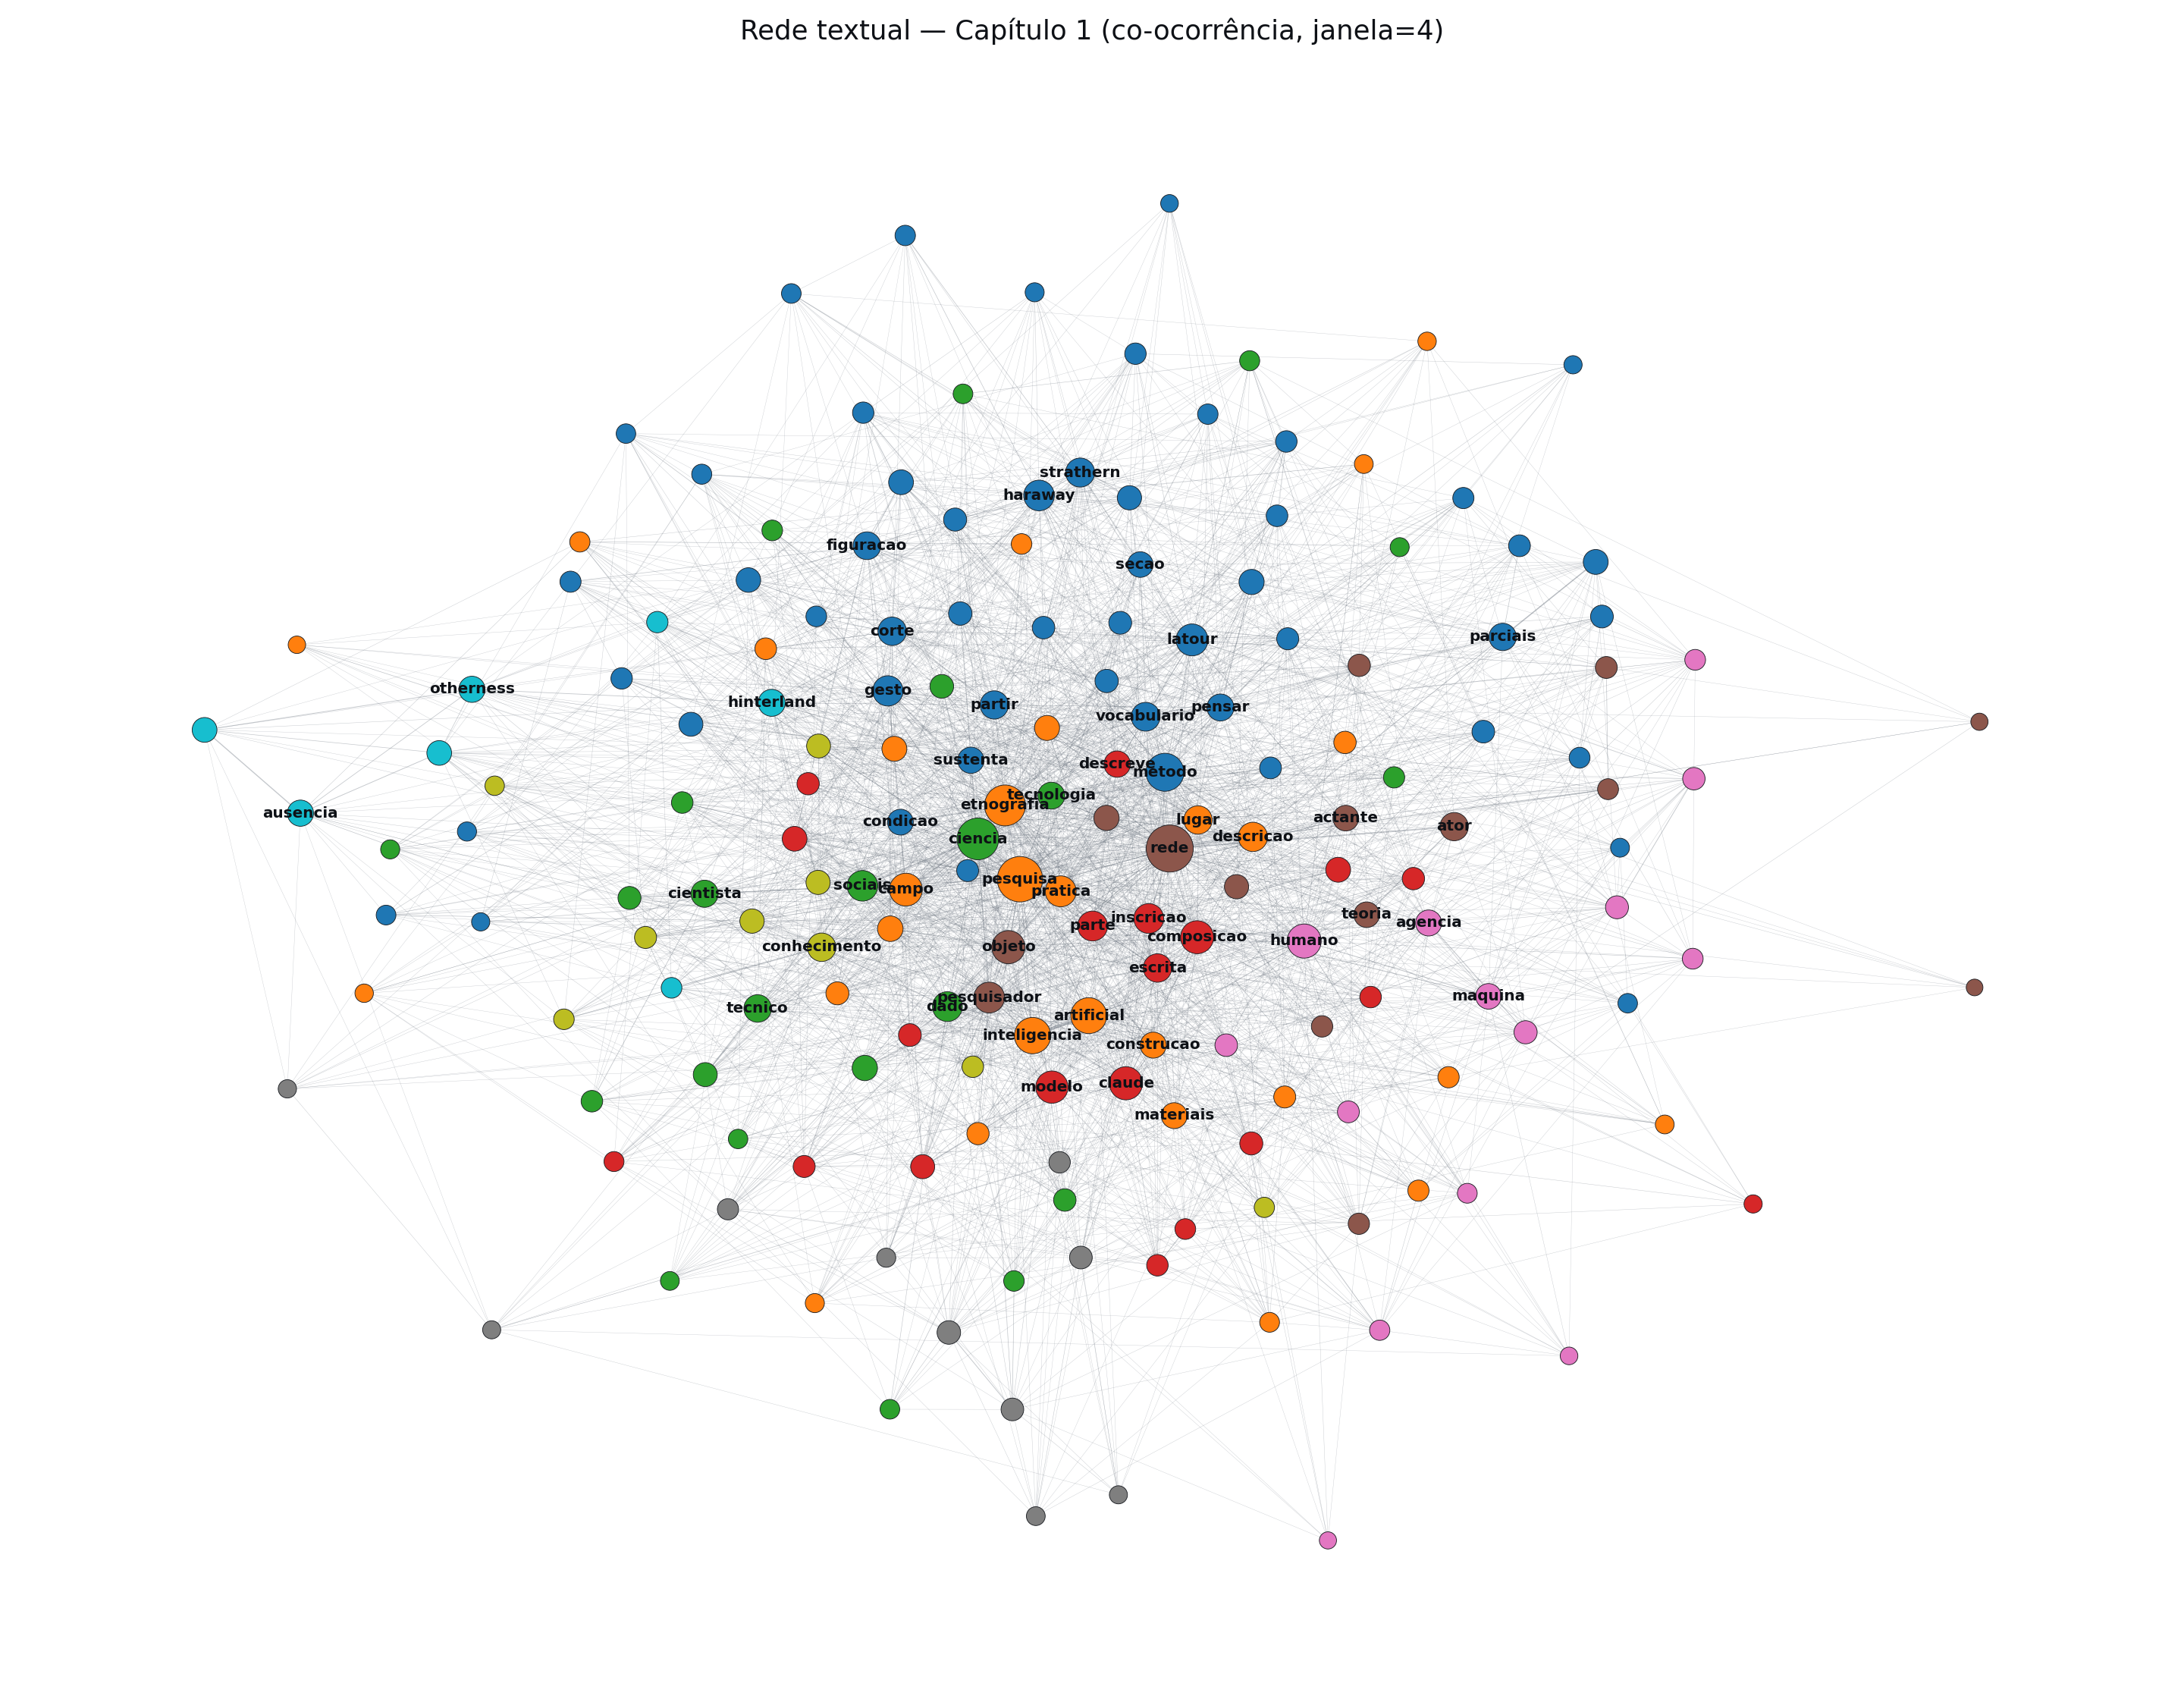
\includegraphics[width=1.0\textwidth,keepaspectratio]{figuras/cap.1/infranodus_cap1_network.png}
\caption[Rede textual completa do capítulo~\ref{capitulo1} (análise de rede textual)]{Rede textual completa do capítulo~\ref{capitulo1} (análise de rede textual, segundo \textcite{paranyushkin2019infranodus}). O grafo resulta de janela deslizante de 4 \textit{tokens} sobre o texto pré-processado (remoção de \textit{stopwords}, comandos \LaTeX, lematização leve), com pesos decrescentes pela distância (3-2-1). Os nós são os 180 termos de maior frequência mantidos no maior componente conectado após a filtragem de arestas com peso $<2$; o tamanho do nó é proporcional ao \textit{degree} ponderado e a cor indica a comunidade detectada por Louvain ponderado. Esta vista privilegia a estrutura geral do capítulo, incluindo termos periféricos e pontes entre tópicos. Arquivos auxiliares (\texttt{.gexf} para \texttt{Gephi}, CSVs, métricas e relatório) em \texttt{infranodus/} no repositório \url{https://github.com/julianehelanski/tecno-etnografia-centro-ia}.}
\label{fig:infranodus-cap1-network}
\end{figure}

A segunda inscrição reduz o grafo ao seu esqueleto semântico (figura~\ref{fig:infranodus-cap1-focus}) e me devolve, com clareza, a resposta à pergunta inicial. Mantenho apenas os 100 termos com maior \textit{degree} ponderado e as arestas mais densas. Os termos com maior peso são, em ordem, \textit{pesquisa}, \textit{ciência}, \textit{rede}, \textit{pesquisador(a)}, \textit{modelo}, \textit{humano}, \textit{objeto}, \textit{inteligência}, \textit{artificial}, \textit{campo} e \textit{etnografia}. Os termos que mais costuram comunidades distintas, isto é, com maior \textit{betweenness}, são \textit{ciência}, \textit{pesquisa}, \textit{rede} e \textit{pesquisador(a)}: termos genéricos que permitem o trânsito entre os campos conceituais da teoria ator-rede, das ciências sociais e da inteligência artificial. A condição de \textit{ponte}, no sentido que \textcite{Latour1986Visualization} dá ao termo, parece coincidir aqui com a condição de \textit{tradutor} no sentido latouriano mais amplo \parencite{Latour2011CienciaEmAcao}. A detecção de comunidades estabilizou seis tópicos latentes:\footnote{Os rótulos abaixo correspondem aos quatro a seis termos de maior \textit{degree} dentro de cada comunidade; preservo a forma lematizada produzida pelo \texttt{script} para evitar tradução interpretativa precoce.} (i)~\textit{escrita} e \textit{composição} em torno de \textit{pesquisador}, \textit{modelo}, \textit{objeto}, \textit{Claude}; (ii)~campo conceitual ator-rede em torno de \textit{rede}, \textit{Latour}, \textit{agência}, \textit{ator}, \textit{diagrama}, \textit{distribuída}; (iii)~ciências sociais e campo em torno de \textit{ciência}, \textit{sociais}, \textit{dado}, \textit{conhecimento}, \textit{cientista}; (iv)~IA e etnografia em torno de \textit{pesquisa}, \textit{inteligência}, \textit{artificial}, \textit{etnografia}, \textit{construção}, \textit{técnico}; (v)~humano-máquina-método em torno de \textit{humano}, \textit{método}, \textit{existência}, \textit{máquina}, \textit{parcial}; (vi)~um \textit{cluster} periférico em torno de \textit{Simondon}, \textit{técnica} e \textit{alienação}.

\begin{figure}[H]
\centering
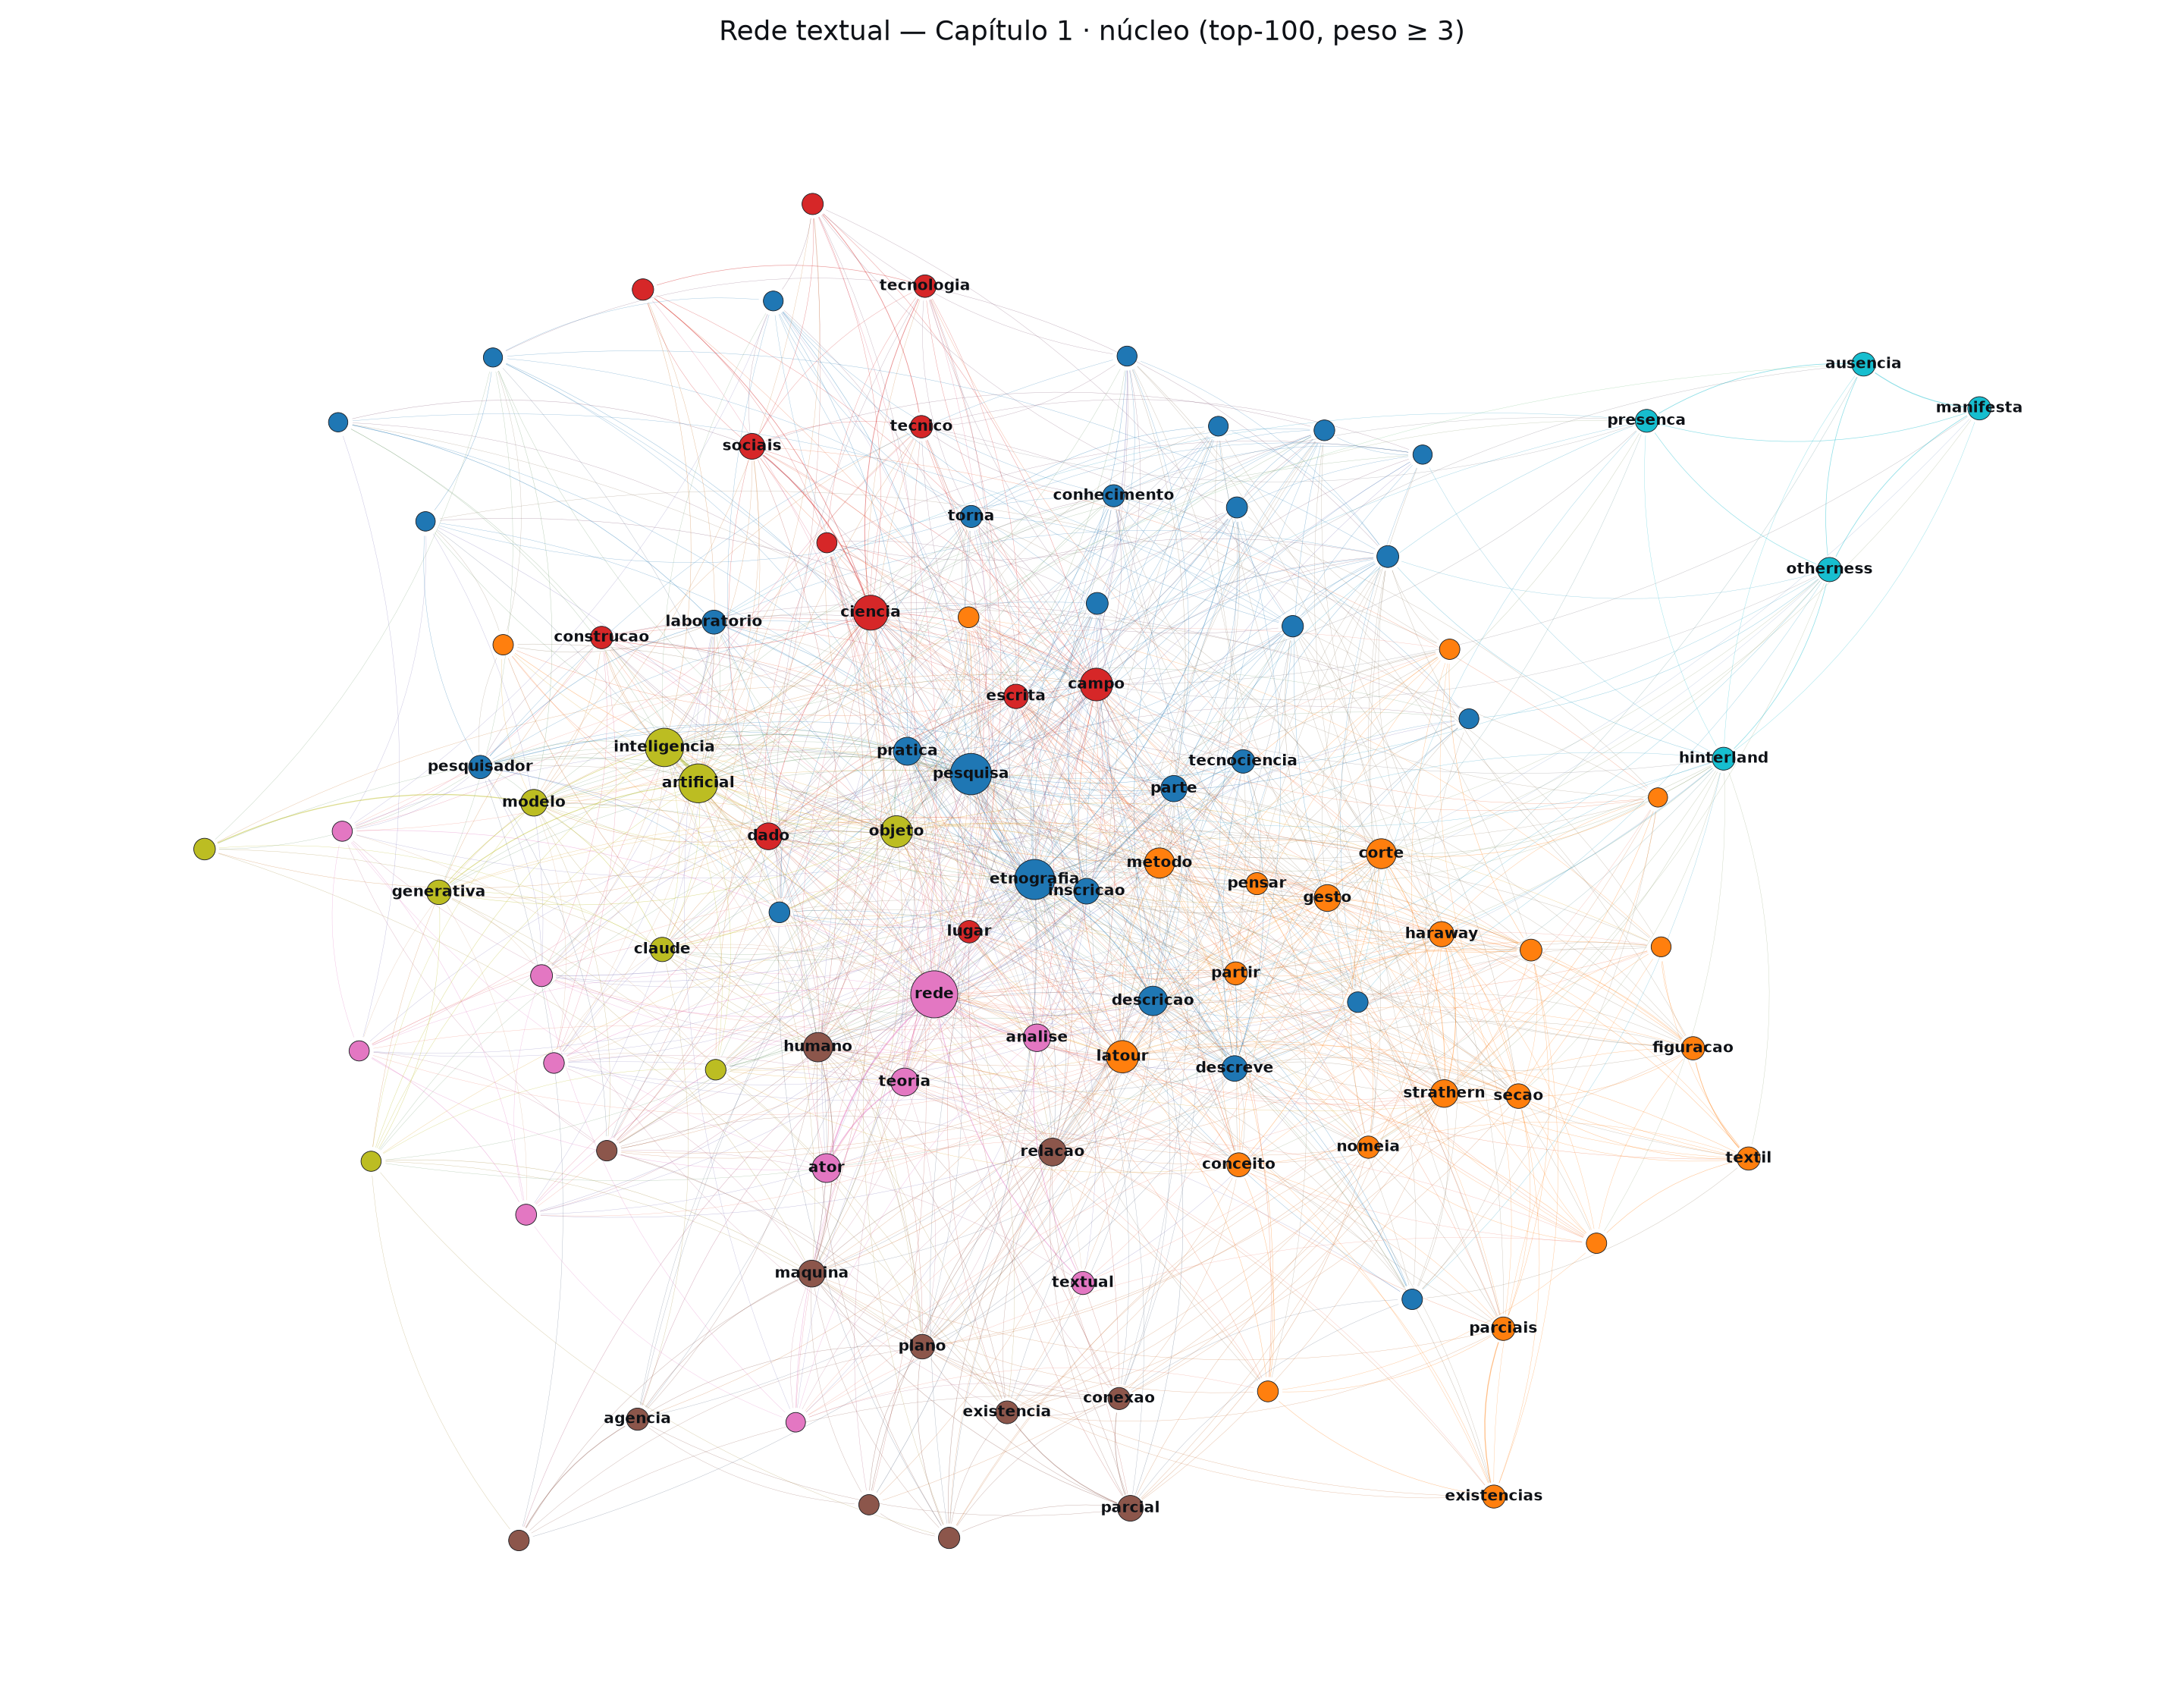
\includegraphics[width=1.0\textwidth,keepaspectratio]{figuras/cap.1/infranodus_cap1_focus.png}
\caption[Núcleo da rede textual do capítulo~\ref{capitulo1} (análise de rede textual)]{Núcleo da rede textual do capítulo~\ref{capitulo1} (análise de rede textual). Os nós são os 100 termos com maior \textit{degree} ponderado; o tamanho do nó é proporcional ao \textit{degree}; a cor indica a comunidade detectada por Louvain ponderado; arestas com peso $\geq 3$. Comparada à figura~\ref{fig:infranodus-cap1-network}, esta vista retém apenas o esqueleto semântico do capítulo, ou seja, os conceitos mais centrais e suas conexões fortes, sem a periferia. Versão de alta resolução, arquivo \texttt{.gexf} para o \texttt{Gephi} e relatório completo disponíveis em \texttt{infranodus/} no repositório \url{https://github.com/julianehelanski/tecno-etnografia-centro-ia}.}
\label{fig:infranodus-cap1-focus}
\end{figure}

A terceira inscrição muda o critério de peso (figura~\ref{fig:infranodus-cap1-focus-pmi}). Até aqui, o tamanho dos nós e a densidade das arestas refletiram a contagem ponderada, métrica que tende a inflar conceitos onipresentes cuja associação com qualquer outro termo é estatisticamente trivial. Aqui, ranqueio os mesmos 100 nós segundo critérios informacionais: o tamanho passa a ser proporcional ao \textit{PageRank}, que mede a centralidade na rede em vez da contagem bruta, e as arestas são filtradas pelo \textit{Normalized Pointwise Mutual Information} (NPMI), que retém apenas co-ocorrências surpreendentes dadas as frequências marginais de cada termo. O efeito é redistribuição da hierarquia textual: conceitos pouco frequentes e estrategicamente posicionados sobem para o primeiro plano, e termos onipresentes cuja vizinhança é previsível recuam. Quis essa inscrição justamente porque desconfiava da resposta da figura~\ref{fig:infranodus-cap1-focus}: termos como \textit{pesquisa} e \textit{ciência} pesam tanto que arriscam encobrir conexões mais específicas. A leitura comparada das duas figuras me devolve duas listas distintas do que tem peso no meu texto, e a diferença entre elas é informação metodologicamente carregada.

\begin{figure}[H]
\centering
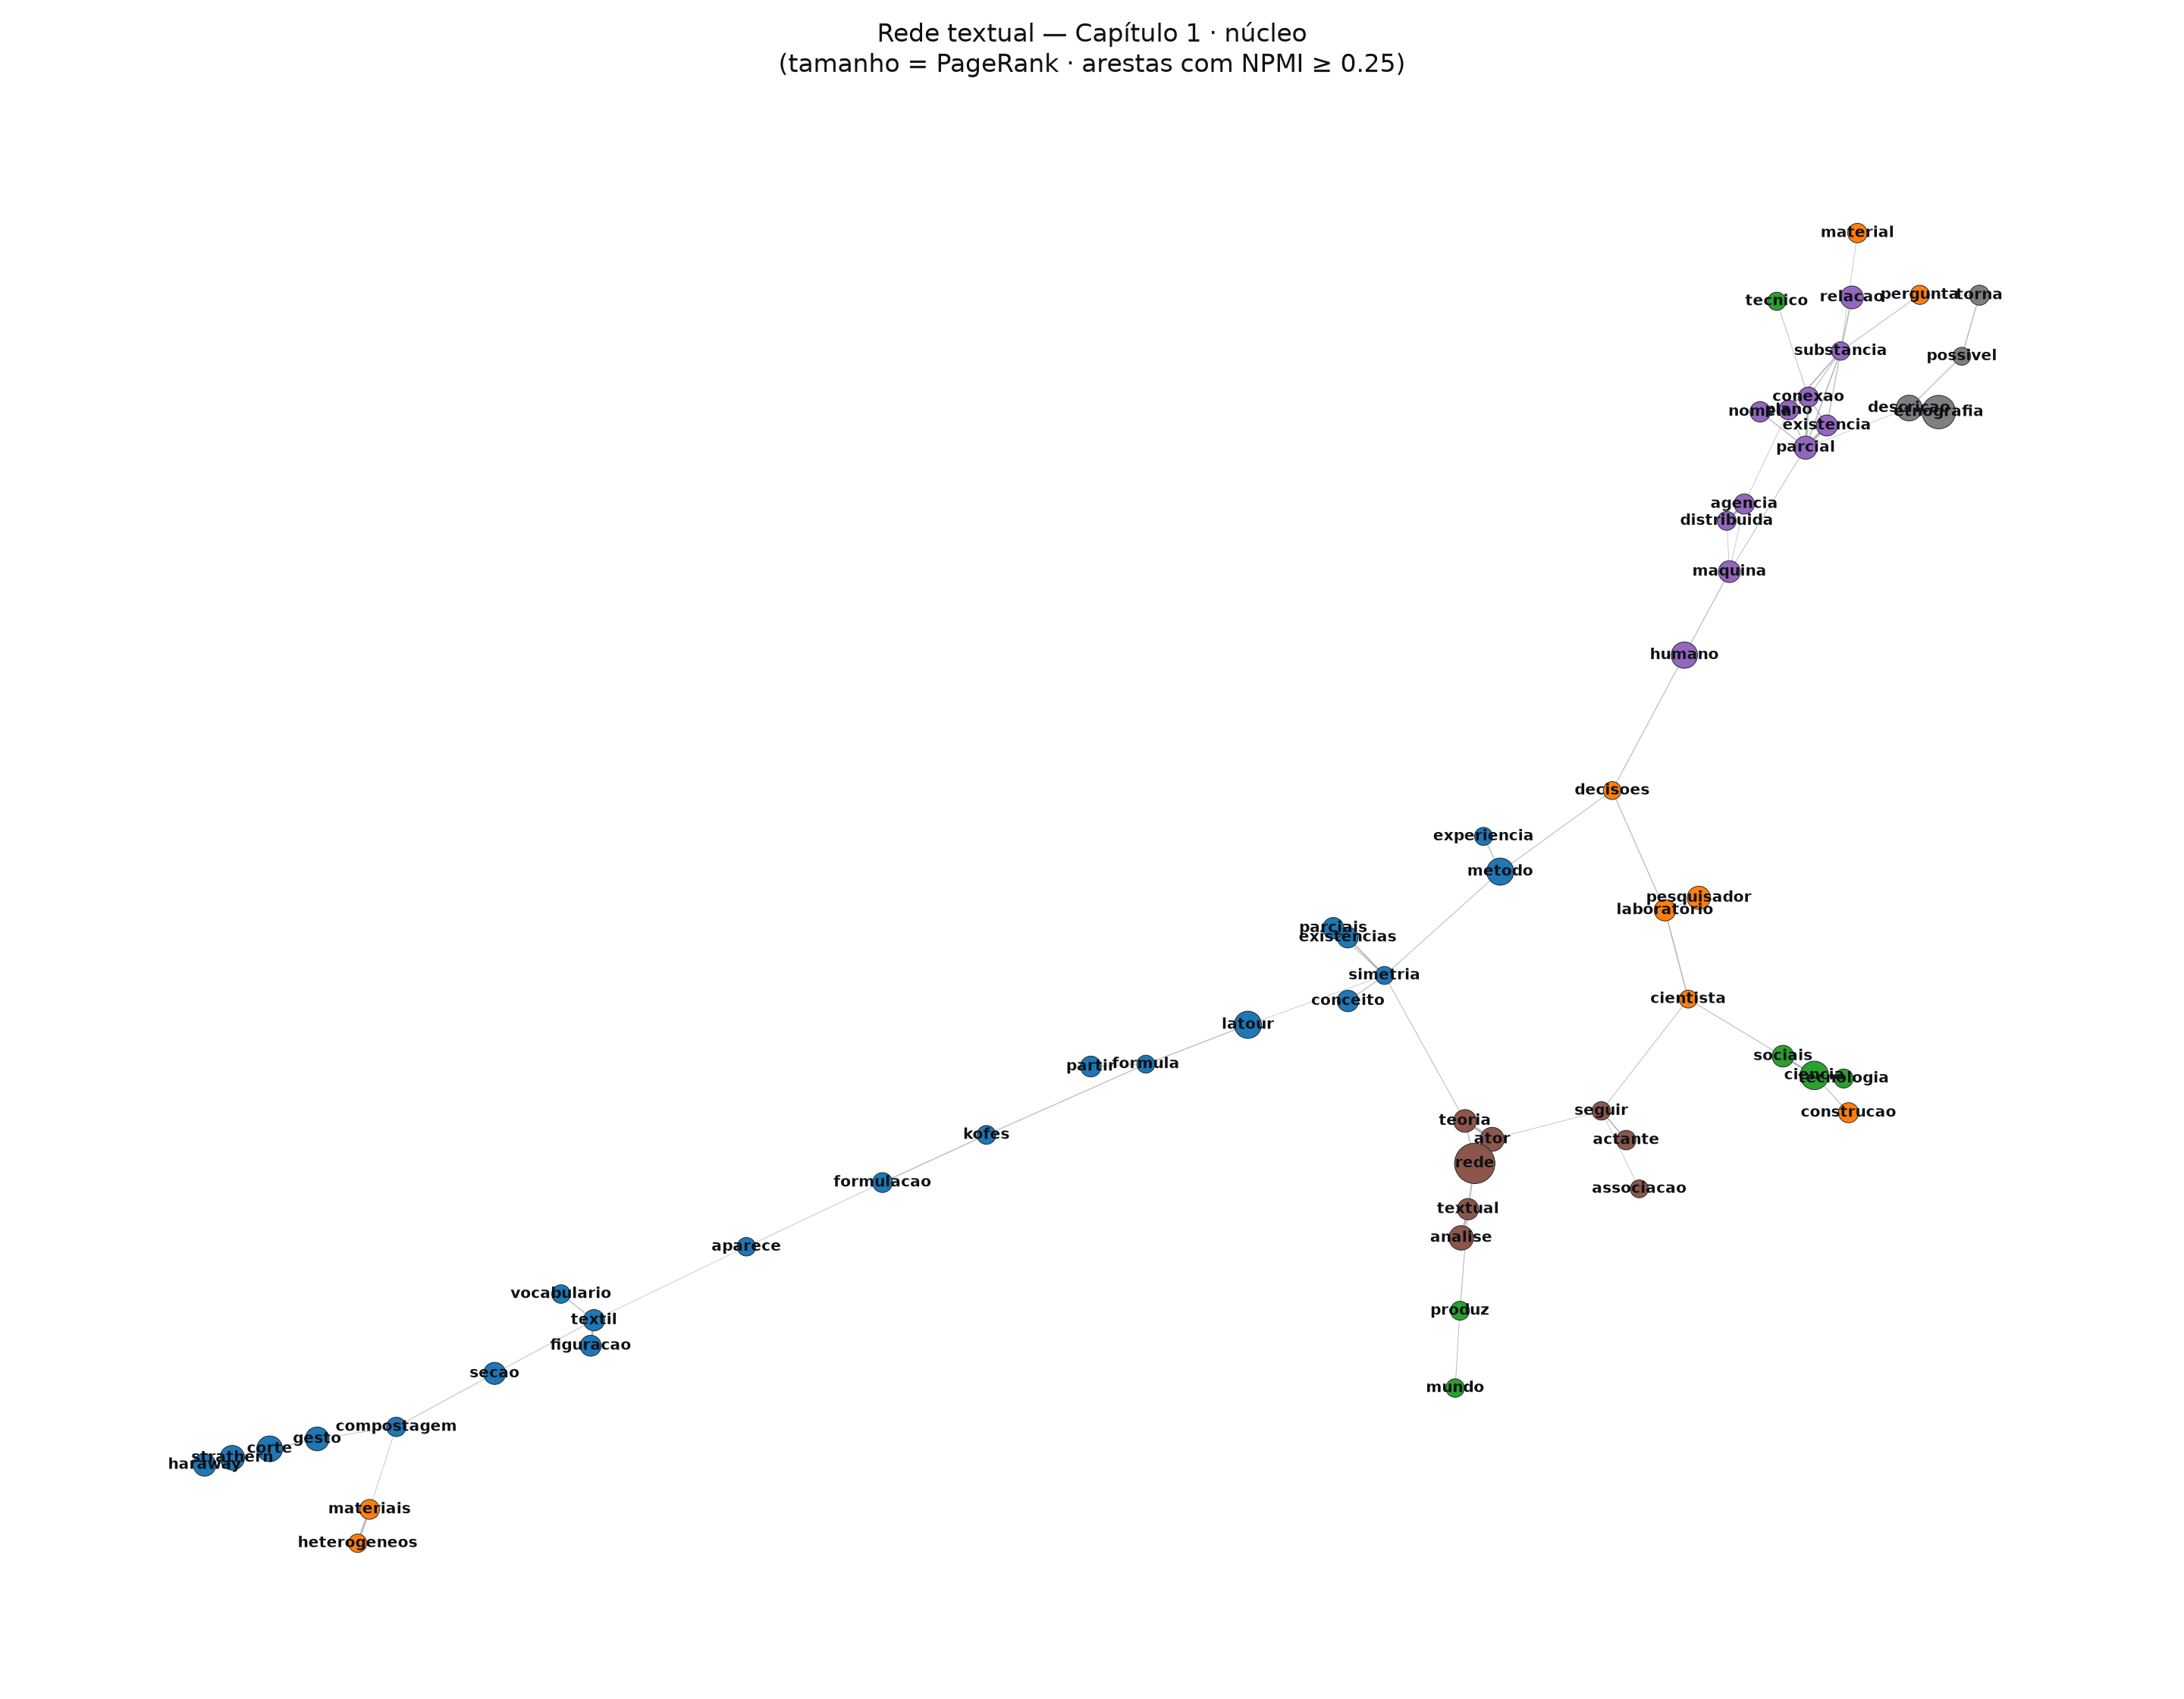
\includegraphics[width=1.0\textwidth,keepaspectratio]{figuras/cap.1/infranodus_cap1_focus_pmi.png}
\caption[Núcleo da rede textual do capítulo~\ref{capitulo1} ponderado por PageRank e NPMI]{Núcleo da rede textual do capítulo~\ref{capitulo1}, ranqueado por critérios informacionais em vez de frequentistas. Os mesmos 100 nós da figura~\ref{fig:infranodus-cap1-focus} são exibidos, mas o tamanho passa a ser proporcional ao \textit{PageRank} (centralidade na rede, em vez de contagem bruta) e as arestas são filtradas pelo \textit{Normalized Pointwise Mutual Information} (NPMI~$\geq 0{,}25$), retendo apenas co-ocorrências surpreendentes dadas as frequências marginais de cada termo. A cor mantém a comunidade Louvain. Esta vista promove conceitos pouco frequentes e estrategicamente posicionados, e deprime termos onipresentes cuja associação com qualquer outro é trivial, funcionando como contraponto à leitura puramente frequentista. Métricas e arquivo \texttt{.gexf} em \texttt{infranodus/} no repositório \url{https://github.com/julianehelanski/tecno-etnografia-centro-ia}.}
\label{fig:infranodus-cap1-focus-pmi}
\end{figure}

\medskip

As três inscrições seguintes mudam de pergunta. Em vez de \enquote{o que se liga a quê}, perguntam \enquote{quando cada conceito entra na minha argumentação, quanto tempo permanece em circulação, e como migra ao longo do capítulo}. Convertem o tempo da leitura, isto é, a ordem dos parágrafos, em eixo de análise. Eu precisava saber se os termos que pesam nas vistas sincrônicas pesam por persistência ou por concentração local, e essa pergunta não tem como ser respondida pelos grafos anteriores.

A quarta inscrição é o Gantt lexical (figura~\ref{fig:trajectory-gantt}). Cada linha do gráfico corresponde a um conceito, e cada barra horizontal marca a vida desse conceito no capítulo, do parágrafo de entrada ao parágrafo de saída. A inscrição me devolve informação que os grafos sincrônicos não ofereciam: existem conceitos que abro cedo e mantenho até o fim, existem conceitos que entram tarde e ficam pouco tempo, e existem conceitos que circulam por janela estreita de parágrafos antes de desaparecer. A leitura do Gantt traz autocrítica imediata: alguns dos termos com maior \textit{degree} nas vistas sincrônicas só existem em fração curta do capítulo, o que sugere que sua centralidade estrutural disfarça uma centralidade local. A inscrição expõe essa diferença sem que eu precise tematizá-la em prosa.

\begin{figure}[H]
\centering
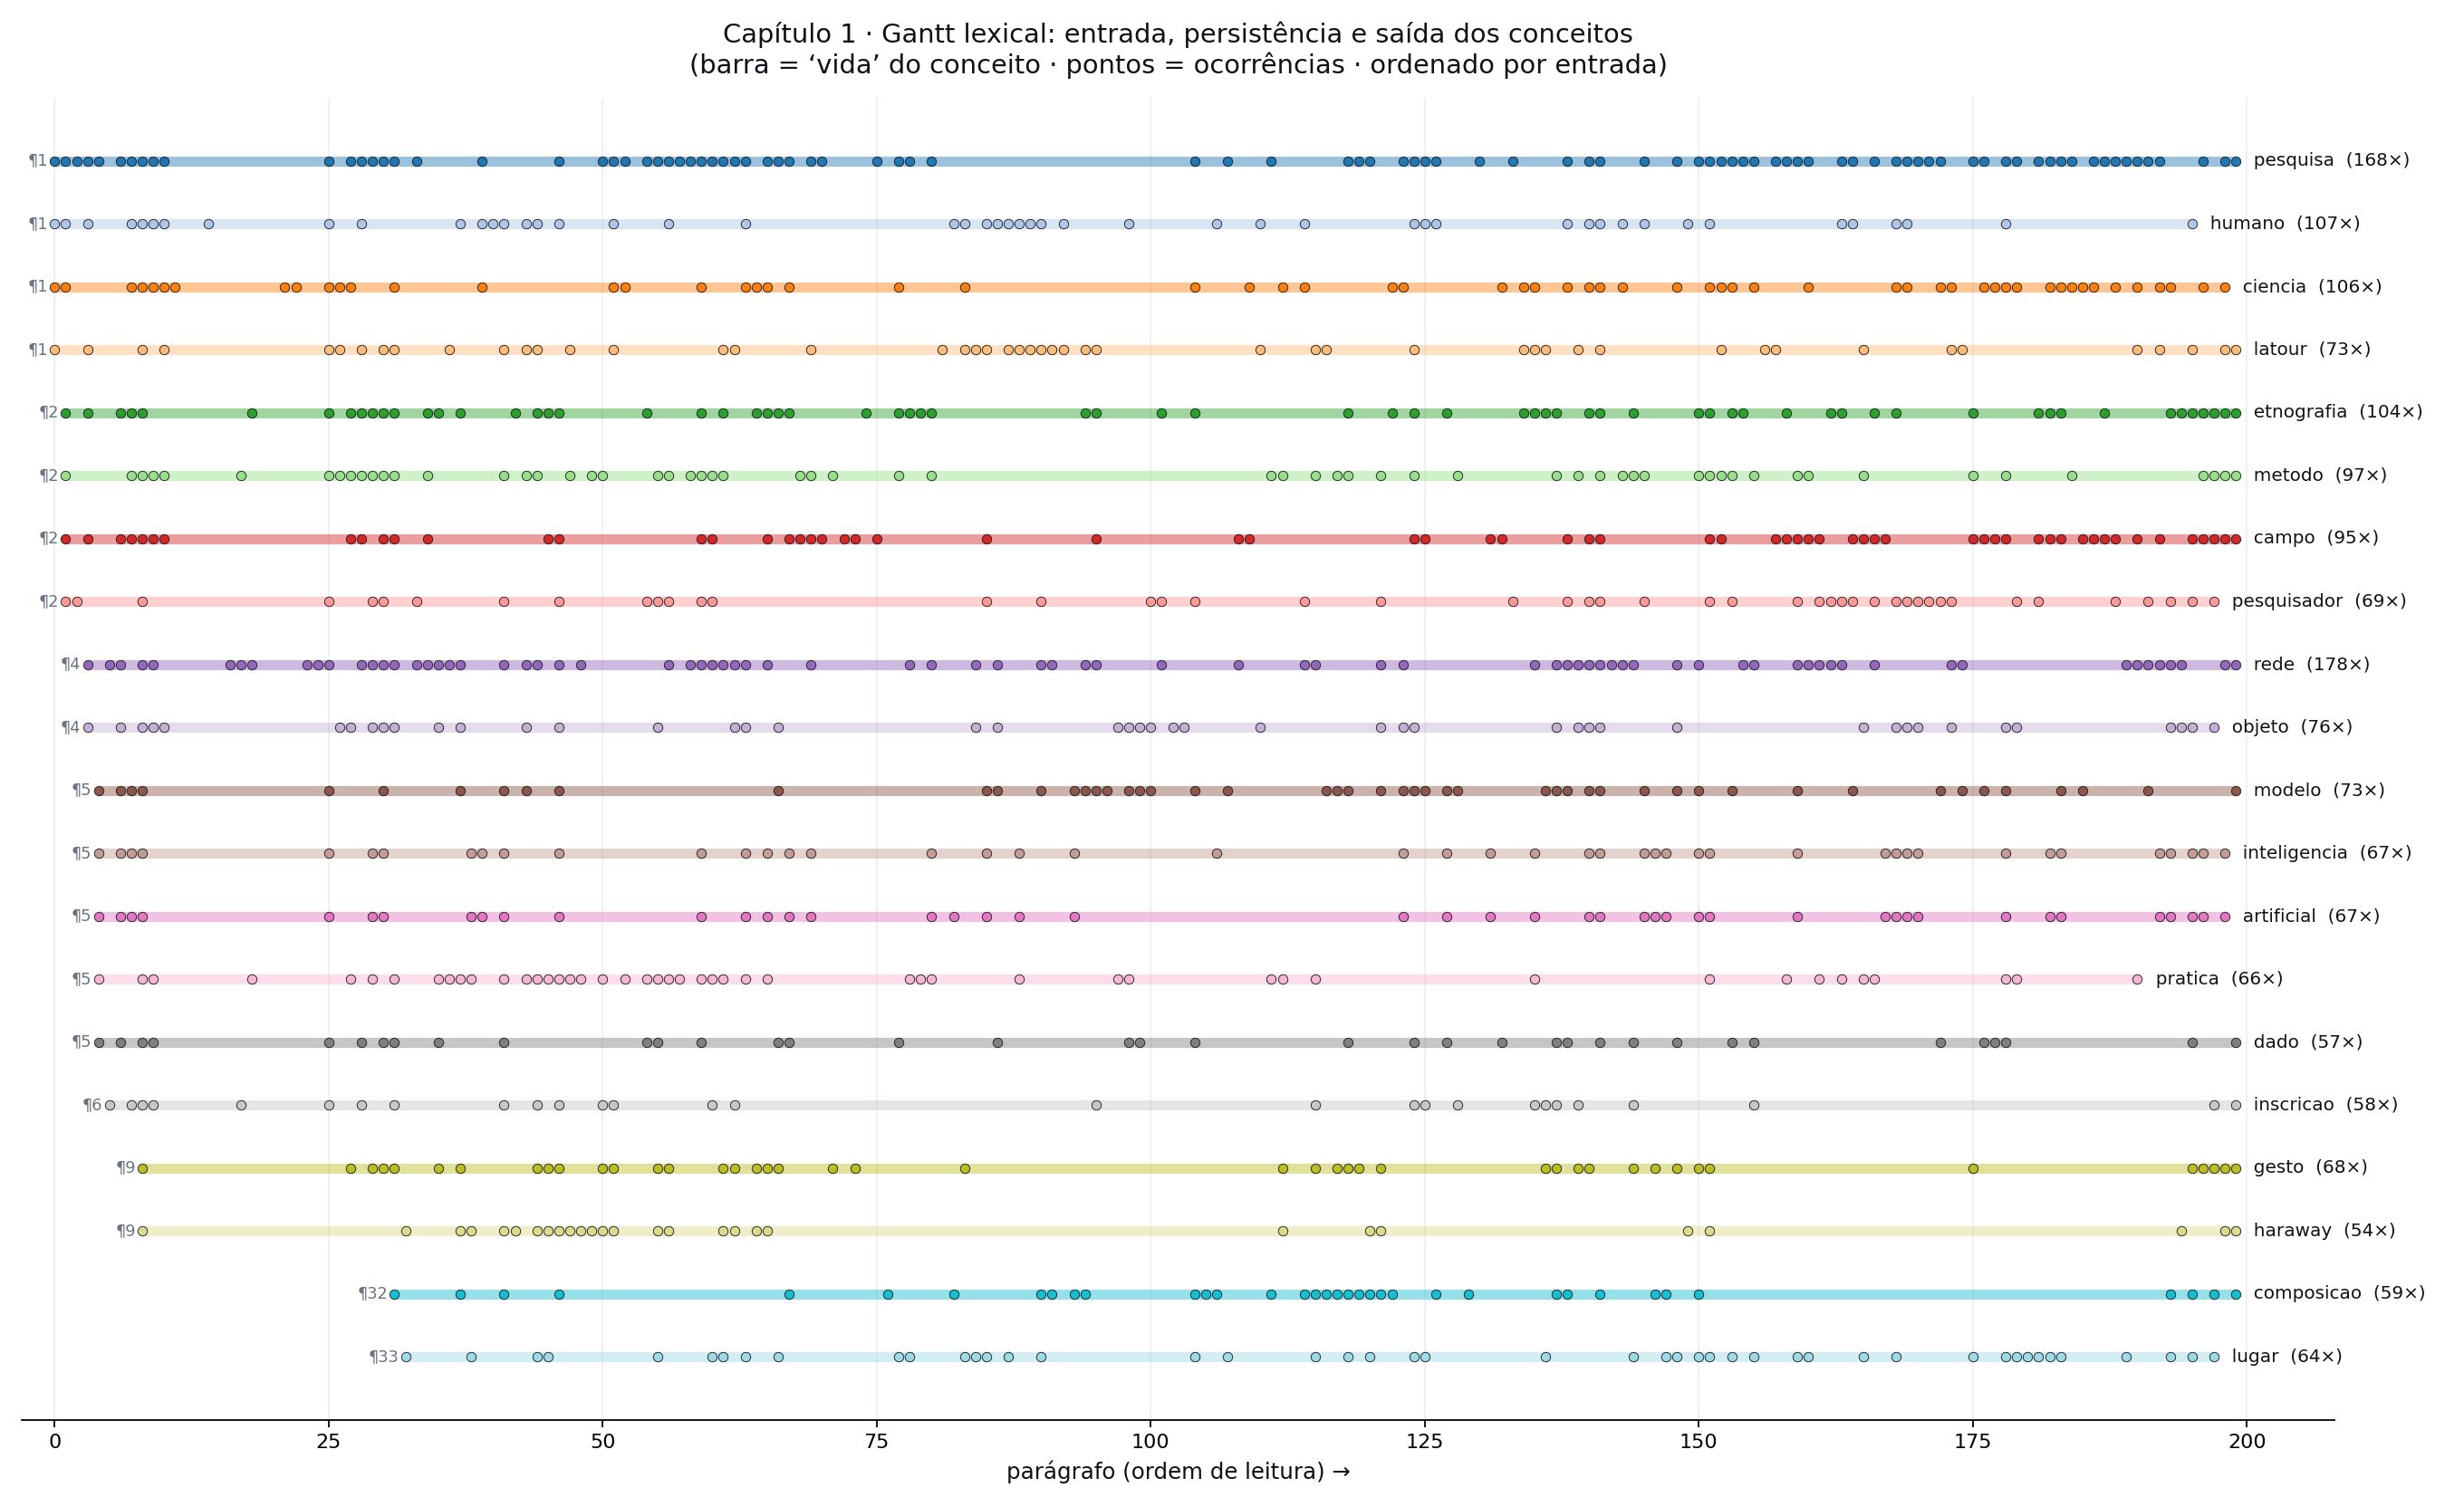
\includegraphics[width=1.0\textwidth,keepaspectratio]{figuras/cap.1/trajectory_gantt.png}
\caption[Gantt lexical do capítulo~\ref{capitulo1}: entrada, persistência e saída dos conceitos]{Gantt lexical do capítulo~\ref{capitulo1}. Cada linha corresponde a um dos 20 conceitos de maior frequência, excluídos termos genéricos e o marcador \texttt{claude}; o eixo horizontal é a ordem de leitura em parágrafos. A barra colorida marca a vida do conceito no capítulo, do parágrafo de primeira aparição (rótulo \P\textit{n}) ao último; os pontos sobre a barra indicam cada ocorrência; o número entre parênteses à direita é a contagem total. As linhas estão ordenadas por parágrafo de entrada, evidenciando a sequência em que cada noção é convocada e por quanto tempo permanece em circulação. Gerado pelo \textit{script} \texttt{narrative\_trajectory.py}, disponível em \url{https://github.com/julianehelanski/tecno-etnografia-centro-ia/tree/main/infranodus}.}
\label{fig:trajectory-gantt}
\end{figure}

A quinta inscrição refina a anterior por meio do fluxo aluvial (figura~\ref{fig:trajectory-alluvial}). Em vez de exibir cada conceito como entidade isolada, particiono o capítulo em oito segmentos sequenciais e mostro, em cada segmento, os cinco termos de maior frequência local. Faixas translúcidas conectam um termo a si mesmo quando ele persiste no \textit{top}-5 entre segmentos adjacentes, e setas marcam estreias.
O efeito visual é o de sucessão de paisagens conceituais que se sobrepõem parcialmente: alguns termos atravessam o capítulo inteiro, outros aparecem em apenas um segmento, e existem zonas de transição em que conjuntos conceituais inteiros são substituídos. A inscrição responde à pergunta que o Gantt deixa em aberto, qual seja, a de saber o que coexiste com o quê em cada momento da minha argumentação. Ela me mostra que o meu texto tem biografia: conceitos nascem, vivem com outros conceitos, e morrem, e essa biografia é parte do que dá peso aos termos nas vistas sincrônicas.

\begin{figure}[H]
\centering
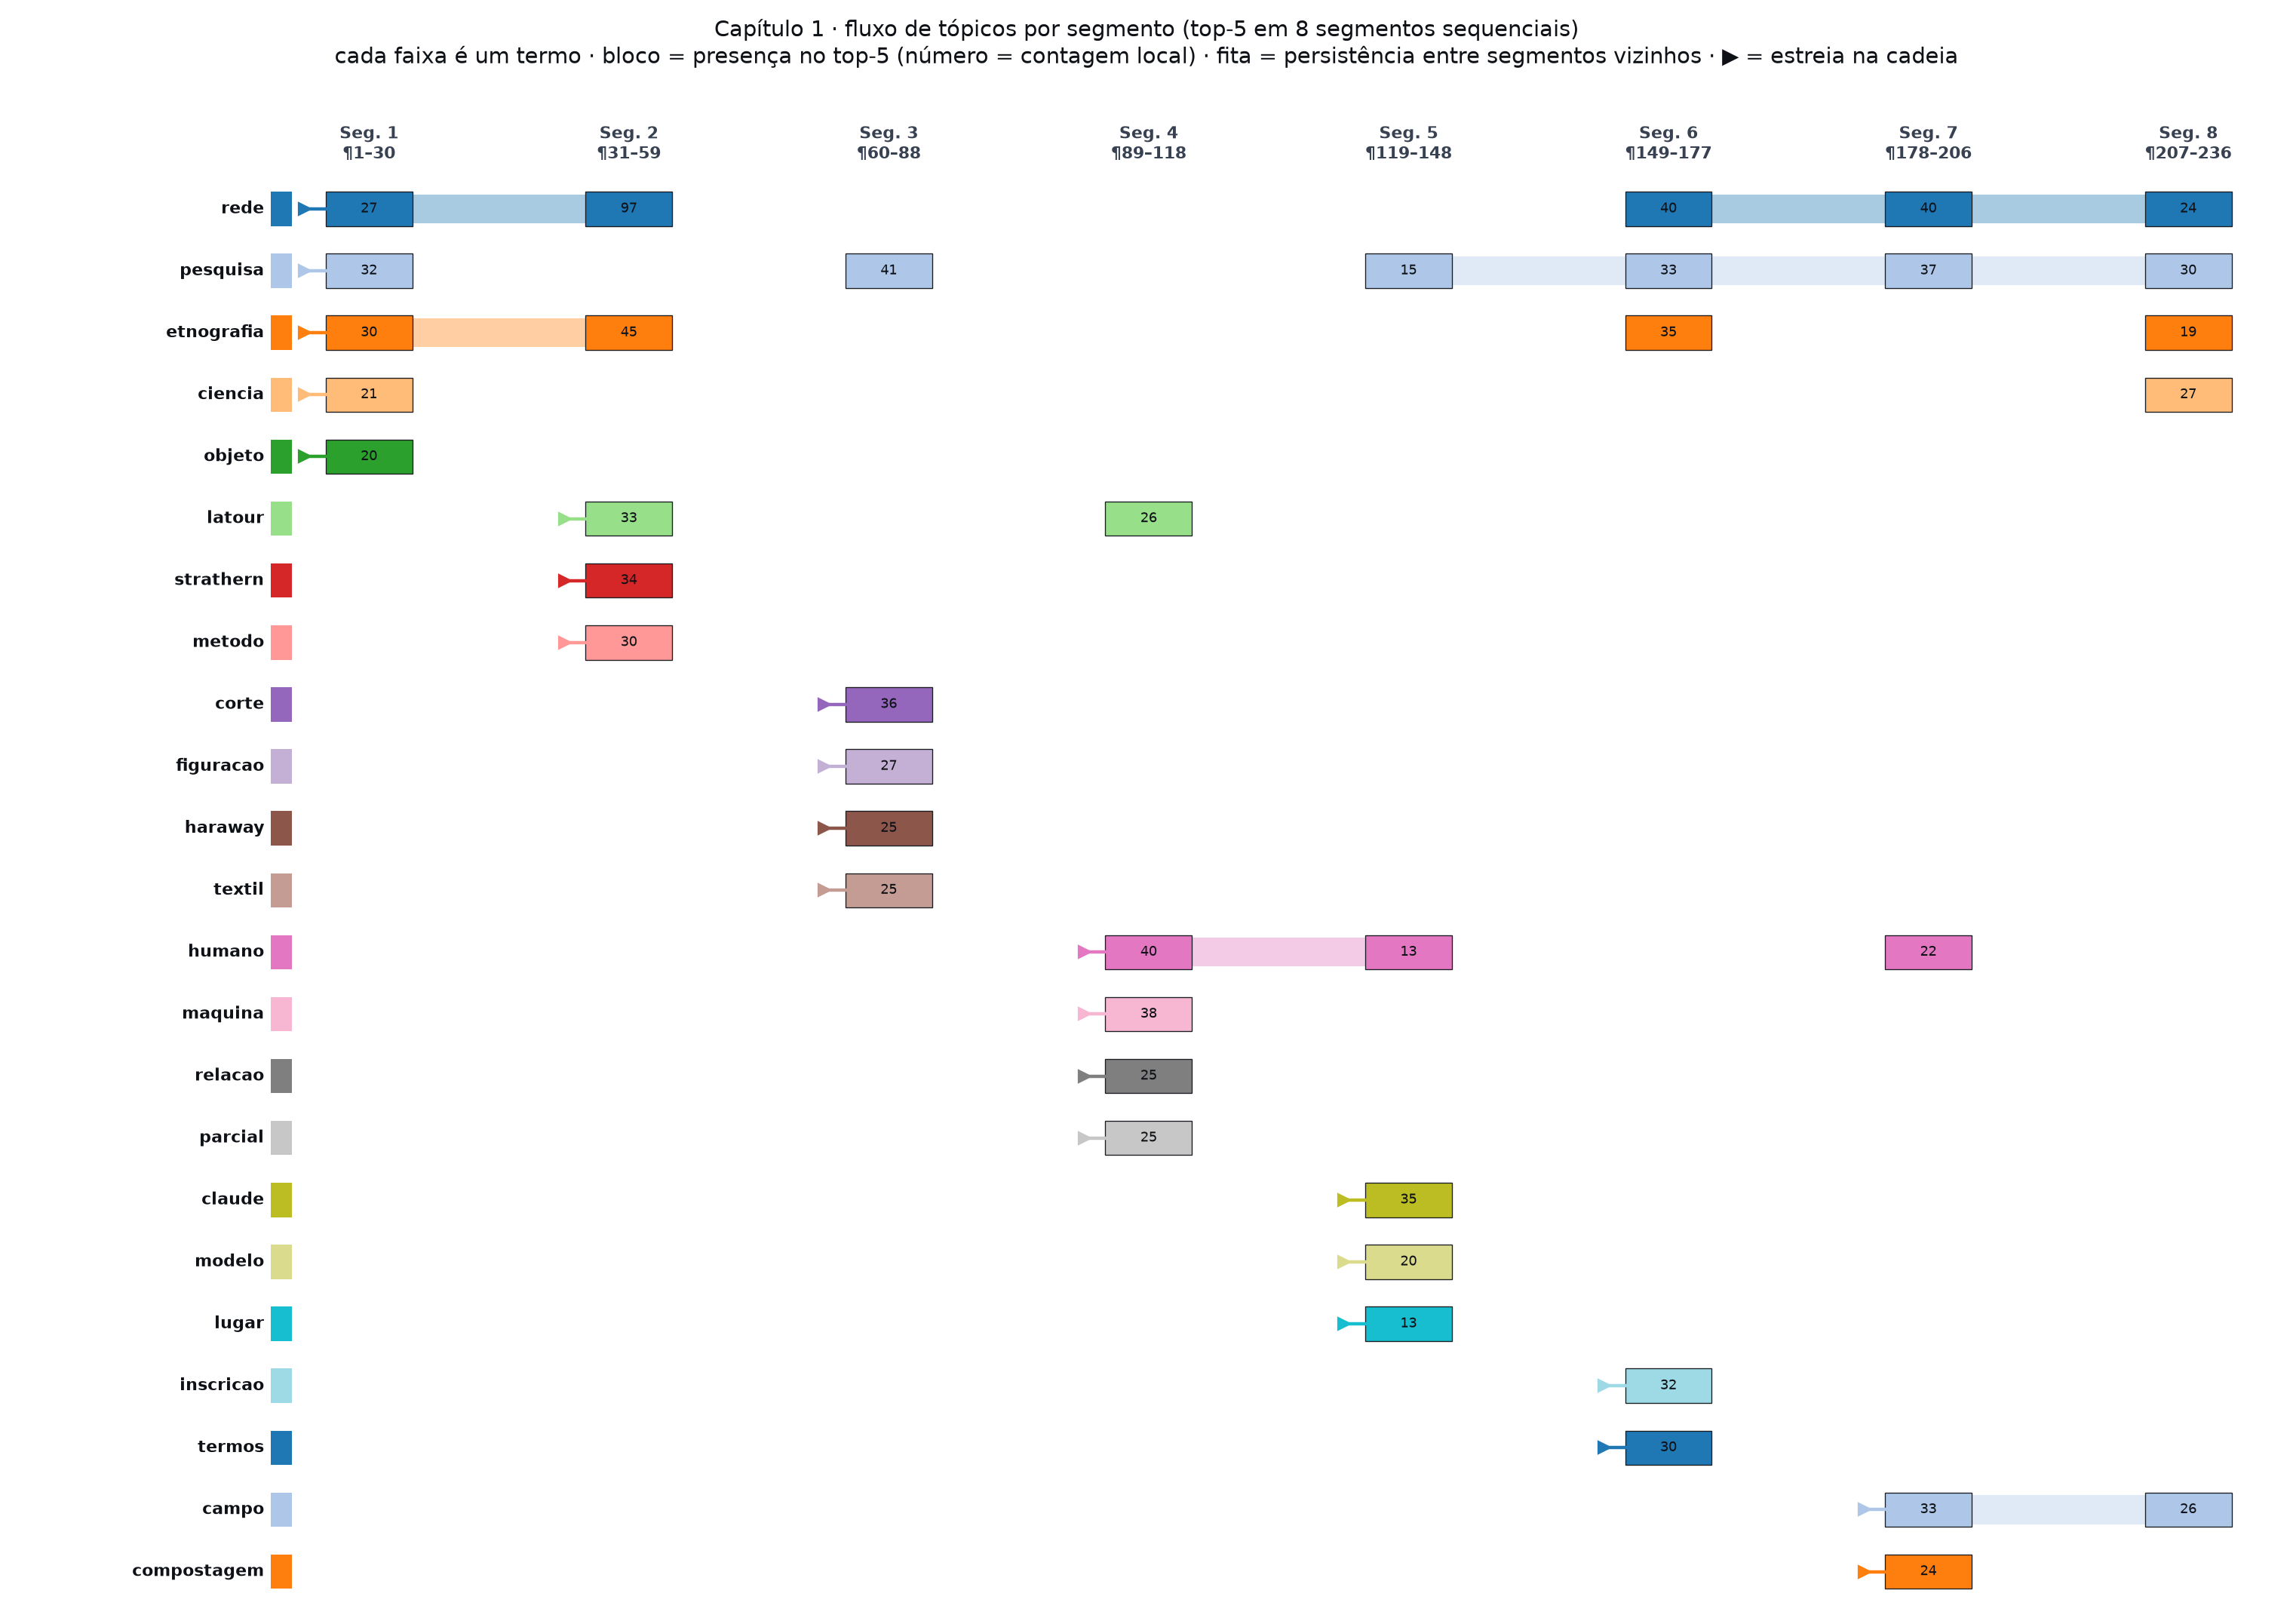
\includegraphics[width=1.0\textwidth,keepaspectratio]{figuras/cap.1/trajectory_alluvial.png}
\caption[Fluxo aluvial de tópicos ao longo do capítulo~\ref{capitulo1}]{Fluxo aluvial do capítulo~\ref{capitulo1}. O capítulo é particionado em 8 segmentos sequenciais de igual extensão em parágrafos (rótulos \P\textit{n}--\P\textit{m} no topo); em cada segmento são listados os 5 termos de maior frequência local (blocos coloridos, com a posição vertical refletindo o \textit{ranking} dentro do segmento). Faixas translúcidas conectam um termo a si mesmo entre segmentos adjacentes quando ele persiste no \textit{top}-5, materializando continuidades temáticas; setas $\blacktriangleright$ assinalam a primeira aparição de um conceito na cadeia. A figura responde à pergunta \enquote{o que se liga a quê ao longo do capítulo} e torna visíveis tanto os tópicos persistentes quanto as entradas tardias e saídas precoces. Gerado pelo \textit{script} \texttt{narrative\_trajectory.py}, disponível em \url{https://github.com/julianehelanski/tecno-etnografia-centro-ia/tree/main/infranodus}.}
\label{fig:trajectory-alluvial}
\end{figure}

A sexta inscrição opera por compressão ainda mais radical (figura~\ref{fig:trajectory-semantic}). Agrupo os parágrafos em \textit{momentos} de cinco parágrafos consecutivos, vetorizo cada momento por TF-IDF sobre unigramas e bigramas, e projeto a sequência inteira em duas dimensões obtidas por PCA aplicado ao resultado de redução prévia por \textit{Truncated SVD}. O que aparece no plano é trajetória: cada ponto é um momento, as setas seguem a ordem de leitura, e a distância entre pontos aproxima a dissimilaridade lexical entre eles. Deslocamentos longos indicam mudanças temáticas; voltas curtas indicam que retomei campo semântico já visitado. Essa última inscrição me devolve, em vista única e legível de cima, o movimento argumentativo do capítulo: posso rastrear, sem precisar reler tudo, em que ponto da exposição abri um problema, em que ponto voltei a ele, e em que momento o capítulo se distanciou mais de seu próprio começo.

\begin{figure}[H]
\centering
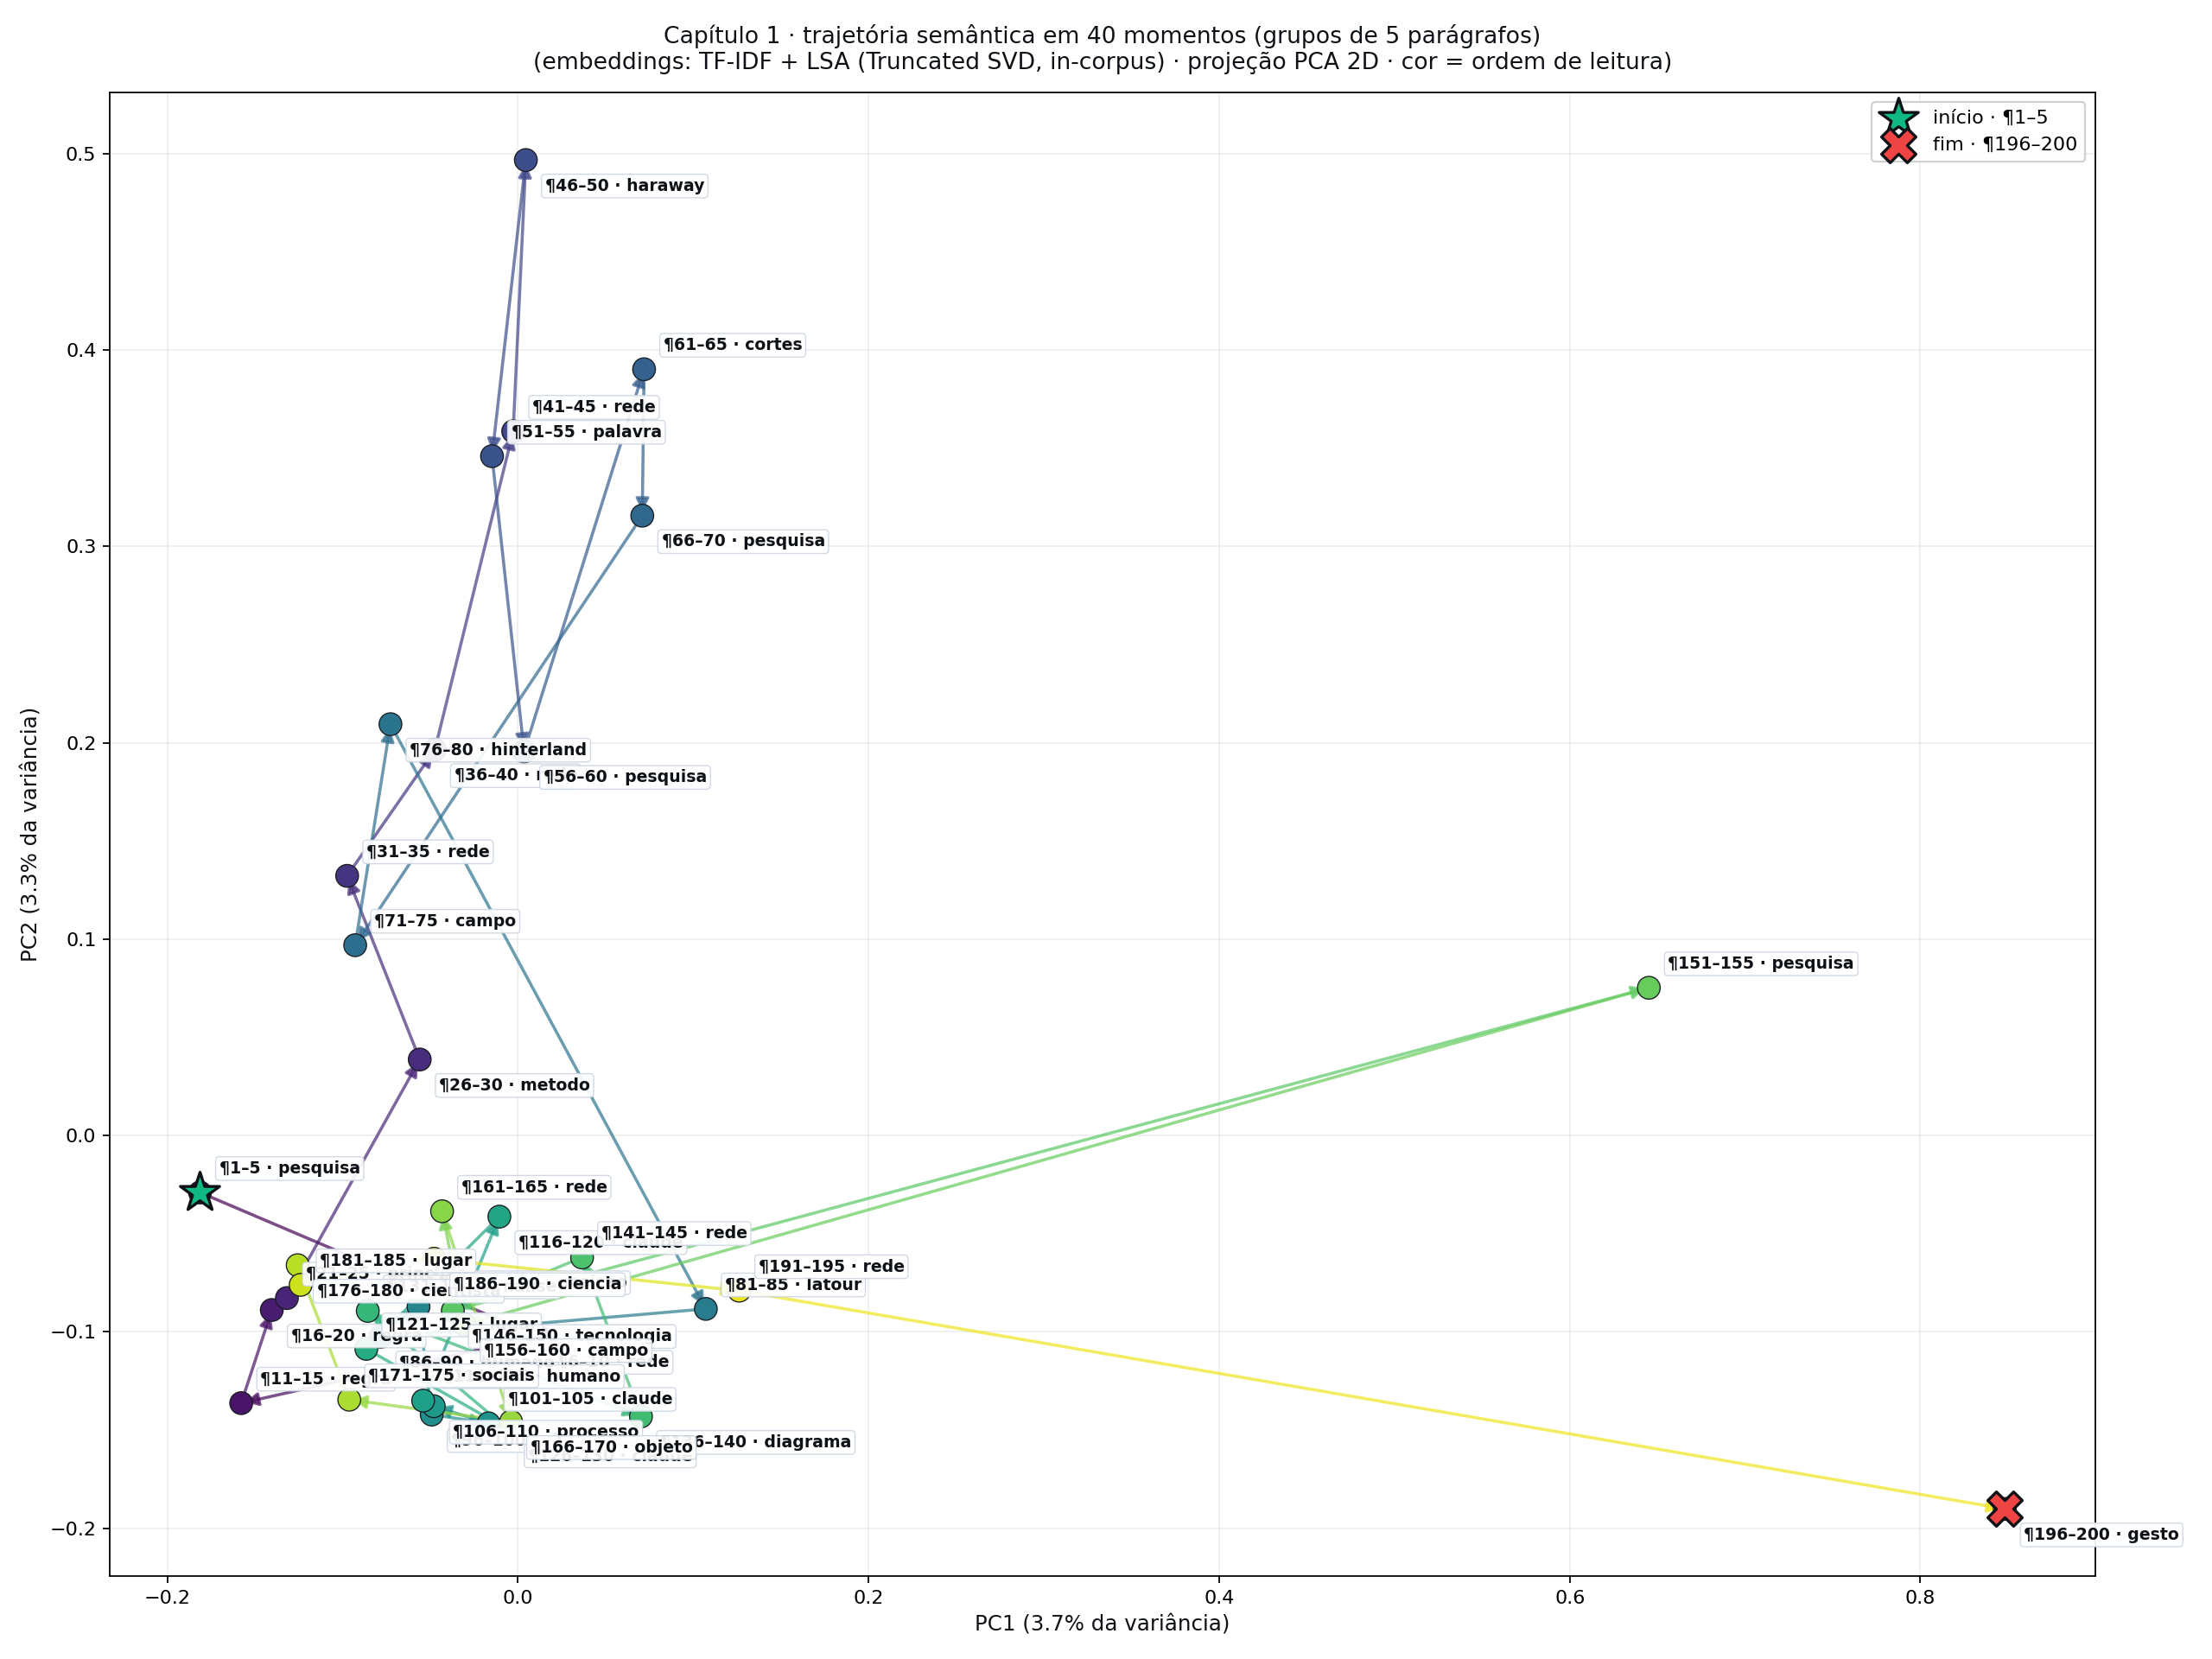
\includegraphics[width=1.0\textwidth,keepaspectratio]{figuras/cap.1/trajectory_semantic.png}
\caption[Trajetória semântica do capítulo~\ref{capitulo1}]{Trajetória semântica do capítulo~\ref{capitulo1}. Os parágrafos são agrupados em \textit{momentos} de 5 parágrafos consecutivos; cada momento é vetorizado por \textit{TF-IDF} (unigramas e bigramas) seguido de redução por \textit{Truncated SVD} (\textit{Latent Semantic Analysis} \textit{in-corpus}, \textit{fallback} usado quando o \textit{sentence-transformer} multilíngue não está disponível) e projetado em duas dimensões por PCA. Cada ponto é um momento, rotulado com o intervalo de parágrafos e o termo dominante; as setas seguem a ordem de leitura, com gradiente \textit{viridis} do início ($\star$ verde) ao fim ($\times$ vermelho). Distâncias no plano aproximam dissimilaridade lexical entre momentos; deslocamentos longos indicam mudanças temáticas, voltas curtas indicam retomada de campo semântico já visitado. O percentual de variância explicada por cada eixo aparece nos rótulos. Gerado pelo \textit{script} \texttt{narrative\_trajectory.py}, disponível em \url{https://github.com/julianehelanski/tecno-etnografia-centro-ia/tree/main/infranodus}.}
\label{fig:trajectory-semantic}
\end{figure}

\medskip

Lidas em série, as seis inscrições tecnocientíficas me devolveram três chamadas de atenção sobre o que pesa e o que conecta no meu texto. A primeira é confirmação modesta: os termos que se mostram centrais nas três vistas sincrônicas coincidem com os conceitos que convoco explicitamente, e os termos com maior intermediação são os mais genéricos do capítulo, o que sugere que minha costura argumentativa está sendo feita por palavras-coringa que ainda esperam ser teorizadas com mais força. A segunda é surpresa que aparece nas seis figuras de modos distintos: as duas comunidades com a ligação ponderada mais fraca entre si são a das ciências sociais (Tópico~iii) e a do par humano-máquina-método (Tópico~v); o Gantt e o aluvial mostram, além disso, que essas duas famílias de termos têm biografias temporais distintas no capítulo, ocupando segmentos parcialmente disjuntos da minha exposição.
A formulação de \textcite{Law2004After} sobre o \textit{method assemblage} me ajuda a nomear o que isso quer dizer: a \textit{Otherness} apagada para que a presença se sustente é, neste capítulo, a conexão entre os dois conjuntos conceituais que ainda preciso fazer trabalhar juntos. A terceira chamada diz respeito ao \textit{cluster} periférico em torno de Simondon: ele aparece na rede expandida (figura~\ref{fig:infranodus-cap1-network}), some no núcleo frequentista (figura~\ref{fig:infranodus-cap1-focus}), reaparece na vista informacional (figura~\ref{fig:infranodus-cap1-focus-pmi}) e ocupa janela curta no Gantt (figura~\ref{fig:trajectory-gantt}), sinalizando promessa teórica que abro aqui e que os capítulos subsequentes precisam costurar à rede maior, sob risco de virar nota de rodapé errante.

Reconheço o paradoxo do gesto. Aplicar análise de rede a um capítulo que invoca a teoria ator-rede arrisca tomar a metáfora pelo método; e a similaridade entre os dois usos da palavra \textit{rede} é superficial, dado que a rede ator-rede é cadeia de associações heterogêneas e ontologicamente plana, e as redes textuais aqui geradas são grafos bidimensionais de co-ocorrências de \textit{tokens} ponderados por proximidade.\footnote{A confusão entre os dois sentidos de \textit{rede} é discutida por \textcite[pp.~129--132]{Latour2007Reassembling}, que distingue \textit{rede} como ferramenta de inscrição e como diagnóstico ontológico. Mantenho a distinção: o que a análise de rede textual e os meus \textit{scripts} de trajetória produzem são inscrições tecnocientíficas; o que minha tese descreve, ela própria, são redes sociotécnicas.} As seis inscrições funcionaram como instrumento de leitura que eu não teria conseguido produzir só com olhos humanos e releituras sucessivas. Cada uma ordena, hierarquiza, inclui e exclui, e o conjunto delas me serviu para localizar o que pesa, o que liga, o que persiste e o que migra na argumentação que costurei. É essa experimentação tecnoetnográfica, e o que ela me devolveu, que justifica sua presença aqui.

\subsection{Cosmotécnica e situacionalidade}

Devo situar essa escolha. Ninguém é obrigado a usar inteligência artificial para fazer pesquisa acadêmica. Há muitas maneiras de fazer uma pesquisa, e nem todas produzem bons resultados, inclusive quando não envolvem tecnologias tão polêmicas quanto a IA. É também verdade que parte dos pesquisadores que recorrem a modelos de linguagem o faz para poupar-se do trabalho intelectual, delegando à máquina o que deveria ser exercício de pensamento,\footnote{Em 6 de março de 2026, o CNPq publicou a Portaria n.º~2.664, que institui a Política de Integridade na Atividade Científica. O Art.~9, inciso~I, alínea~c, determina que pesquisadores declarem o uso de ferramentas de Inteligência Artificial Generativa em qualquer fase do desenvolvimento da pesquisa, especificando a ferramenta utilizada e a finalidade. A alínea~d veda a submissão de conteúdo gerado por IAG como se fosse de autoria humana, atribuindo responsabilidade integral aos autores pelo conteúdo final. Minha tese antecipou, por escolha metodológica, o que a norma agora regula. Disponível em: \url{http://memoria2.cnpq.br/web/guest/view/-/journal_content/56_INSTANCE_0oED/10157/23142775?COMPANY_ID=10132}. Acesso em: 13 mar. 2026.} e os problemas decorrentes dessa delegação já são amplamente conhecidos: textos genéricos, argumentos circulares, referências fabricadas, perda de voz autoral.

Minha tese procura responder a essas três perguntas de modo explícito. O \textit{por que} decorre das condições materiais descritas acima e da coerência com o próprio referencial teórico (estudar existências parciais com uma existência parcial). O \textit{como} está documentado nesta seção e no apêndice~\ref{apendice:colaboracao-ia}. O \textit{qual} atravessa os capítulos que se seguem. Meu fazer-com o \texttt{claude} é, antes de tudo, experimentação antropológica: uma etnógrafa que estuda como cientistas e engenheiros constroem inteligência artificial decide construir sua própria tese com inteligência artificial, submetendo-se às mesmas mediações, opacidades e negociações que observa em seus interlocutores. O gesto é epistêmico e produz conhecimento sobre a IA pela experiência de fazer-com ela, com todos os riscos que esse fazer-com implica.

E se levarmos a sério o argumento de Yuk Hui, esse fazer-com não é generalizável.\footnote{Vicentin conecta a proposta de Simondon de aprofundamento da tecnologia com a defesa de Yuk Hui de que, em lugar de axiomatizar a moral, precisaremos voltar aos modos de conhecimento diferentes que ainda não foram considerados por engenheiros e acadêmicos que trabalham com inteligência artificial \parencite[p.~186]{hui2020tecnodiversidade}. Essa convergência tem peso para meu argumento: se o aprofundamento da IA passa pela conexão entre o fazer técnico especializado e o conhecimento sócio-histórico sobre a tecnologia, então o fazer-com a IA na escrita desta tese pode ser interpretado como experimentação situada nos termos em que Hui concebe a cosmotécnica.} Hui propõe o conceito de cosmotécnica para desafiar a ideia de que a tecnologia seria categoria antropológica única e homogênea: a técnica é sempre a unificação entre uma ordem cósmica e uma ordem moral através de atividades técnicas, e portanto varia ontológica e cosmologicamente entre diferentes sociedades, em lugar de variar apenas funcional ou esteticamente.\footnote{Hui desenvolve o conceito de cosmotécnica em \textit{The Question Concerning Technology in China} \parencite{hui2016china}, onde demonstra que a técnica pode orientar-se pela harmonia com uma cosmologia moral, sem buscar necessariamente a eficiência mecânica. Hui chama essa possibilidade de tecnodiversidade: contra o monotecnologismo moderno, o reconhecimento de que existem múltiplas cosmotécnicas que permitem diferentes formas de vida social, política e estética \parencite{hui2020tecnodiversidade}.}

O quadro herdado da filosofia moderna pós-iluminista trata a tecnologia como conjunto de ferramentas universais e neutras destinadas à exteriorização da memória e à superação dos limites orgânicos. A cosmotécnica recusa essa universalidade: diferentes cosmologias produzem diferentes modos de compor com objetos técnicos, e quem pretende moldar o universal submete o mundo à sua própria cosmovisão. Ora, se há cosmotécnicas situadas, em lugar de a tecnologia, então o modo como eu, antropóloga brasileira, formada na tradição dos estudos de ciência e tecnologia latino-americanos, faço esta tese junto a um modelo de linguagem treinado predominantemente em dados anglófonos para produzir uma tese em português sobre redes tecnocientíficas é, ele próprio, gesto cosmotécnico particular: forma específica de unificar ordem epistêmica e atividade técnica que não se repete em outros contextos, outras tradições, outras cosmologias. A experimentação que documento nestas páginas é, portanto, modo de usar IA na pesquisa acadêmica, situado, parcial e responsável por seus próprios efeitos.

\section{Compostagens: compostar-com e tornar-se-com}
\label{sec:compostagens}

\epigrafe{%
Somos composto, não pós-humanos; habitamos as humusidades, não as humanidades. Filosofica e materialmente, sou compostista, não pós-humanista. Os bichos (humanos e não humanos) estão em devir-com mútuo e em todos os registros de tempo e de coisas, em emaranhados simpoiéticos, em mundificações e desmundicações terrenas, ecológicas e evolutivas do desenvolvimento.}%
{Donna Haraway, \textit{Ficar com o problema: fazer parentes no Chthuluceno}, 2023, p.~191.}

\epigrafe{%
It matters what thoughts think thoughts. It matters what knowledges know knowledges. It matters what relations relate relations. It matters what worlds world worlds. It matters what stories tell stories.}%
{Donna Haraway, \textit{Staying with the Trouble: Making Kin in the Chthulucene}, 2016 \parencite[p.~35]{Haraway2023Ficar}.}

A epígrafe que Haraway formulou \parencite[p.~35]{Haraway2023Ficar} anuncia a prática da compostagem como gesto epistemológico. Quando Haraway escreve que importa quais pensamentos pensam pensamentos, ela credita a Marilyn Strathern a formulação de que importa quais ideias usamos para pensar outras ideias. Esse é o registro próprio desta seção. Cada compostagem aqui descrita é momento em que materiais heterogêneos da minha pesquisa foram postos em camadas e fermentaram juntos, e nessa fermentação aprenderam uns dos outros como pensar uns com os outros. A operação que isto nomeia é distinta do gesto epistêmico do corte trabalhado na seção~\ref{sec:etnografia-heterodoxa}, pois não responde à pergunta sobre onde delimitar a rede para torná-la descritível. Aqui a pergunta é outra, isto é, que materiais empíricos e teóricos vieram parar juntos em minha pesquisa, em que ordem, com que efeitos recíprocos, e por que essas fermentações específicas tornaram possível o tipo de descrição etnográfica que esta tese sustenta. A compostagem trabalha como prática filosófica e material, e a posição de compostista que Haraway reivindica para si \parencite[p.~101]{Haraway2016Staying} é a posição que assumo aqui ao narrar as quatro fermentações que minha pesquisa precisou atravessar.

Minha etnografia acabou produzindo também outro modo de conhecimento que figura como \textit{compostagem}.\footnote{Cheguei ao termo \textit{compostagem} depois de tentar sem sucesso outros nomes para o que essas misturas significaram em minha pesquisa. \textit{Lições} foi a primeira tentativa, e descartei-a porque o vocabulário da lição supõe quem ensina e quem aprende, conteúdos definidos a transmitir, e direção da matéria do mestre para o aprendiz. A pesquisa não se passou assim. \textit{Aprendizagens} carregava o mesmo problema. O que aconteceu foi outra coisa, mais próxima do que \textcite{Haraway2023Ficar} nomeia como compostagem: camadas de materiais heterogêneos postas a fermentar ao longo dos anos, em que nenhum dos elementos pôde ser identificado como o conteúdo a ser transmitido nem como a posição que ensinava. Quatro deslizamentos da palavra organizam meu gesto argumentativo nesta seção. O primeiro é o gesto de Haraway de propor o composto no lugar do pós-humano: \enquote{somos húmus, não Homo, não anthropos; somos compostagem, não pós-humanos} \parencite[p.~32]{Haraway2016Staying}. A formulação foi sugerida a Haraway por Rusten Hogness e a autora descreve seu encontro com ela como pular numa pilha vermicular: \enquote{I jumped into that wormy pile} \parencite[p.~32]{Haraway2016Staying}. A figura recusa o humano-como-Homo em favor do humano-como-húmus, território fértil em que matérias heterogêneas se encontram e se transformam umas às outras. O segundo é a sympoiese, palavra que Haraway adota a partir da tese de Beth Dempster sobre sistemas \enquote{coletivamente produtores} sem fronteiras espaciais ou temporais autodefinidas, e que ela traduz como \textit{making-with}, fazer-com, em contraste com a autopoiese: \enquote{Sympoiesis is a simple word; it means `making-with.' Nothing makes itself; nothing is really autopoietic or self-organizing} \parencite[p.~58]{Haraway2016Staying}. Nada se faz sozinho, e o fazer é sempre em companhia. O terceiro é o par compostar-decompor, formulado por Haraway como prática conjunta de \textit{critters} humanos e não humanos que se compostam e decompõem uns aos outros, em todo tempo e matéria. A compostagem é gesto de juntar e gesto de desfazer, e nesse duplo gesto se ganha a fertilidade do composto. O quarto é a posição que Haraway reivindica: \enquote{I am a compostist, not a posthumanist} \parencite[p.~101]{Haraway2016Staying}. Compostista nomeia prática filosófica e material em curso, em lugar de identidade estabilizada. Dois traços do vocabulário haraweano importam para o uso que faço aqui. O primeiro é a metáfora da pilha quente. Haraway descreve sua leitura de Strathern como \enquote{I compost my soul in this hot pile} \parencite[p.~34]{Haraway2016Staying}, formulação que a tradução brasileira gloseia como \enquote{compostagem intelectual} e que o original nomeia em chave mais visceral, da pilha em fermentação. O segundo é a descrição que Haraway faz do próprio livro nos seus agradecimentos: \enquote{Cooking over many years, the compost pile of colleagues, students, and friends who have made this book possible is promiscuous, layered, and hot} \parencite[p.~ix]{Haraway2016Staying}. Cozinhando ao longo dos anos, em camadas, promíscua e quente: nesse sentido convoco aqui a compostagem para nomear o que aconteceu na minha pesquisa. Cada compostagem desta seção inscreve um momento em que materiais inicialmente mantidos separados pelo desenho da pesquisa precisaram ser postos a fermentar juntos, e em que essa fermentação implicou também a decomposição das partições prévias. A compostagem que mobilizo aqui tem afinidade com a articulação que Haraway desenvolve em torno de \textit{thinking-with} como \textit{becoming-with} \parencite[p.~33]{Haraway2016Staying}: pensar com funciona como tornar-se com, em vez de funcionar como aprender com.} As compostagens são um tipo de contribuição analítica desta tese para a etnografia de práticas tecnocientíficas envolvendo inteligência artificial, em especial a pesquisa em IA feita pelos pesquisadores, com eles e com IA (feita por mim com inteligência artificial). Essas compostagens não estavam previstas no desenho da pesquisa, e emergiram do encontro entre meu campo e os referenciais teóricos que convoquei ao longo do percurso. Cada uma nomeia uma mistura específica de materiais heterogêneos que precisaram fermentar juntos para que a descrição se tornasse possível. A primeira composta a regra latouriana de estudar a ciência em construção com a dispersão característica da pesquisa em IA, na qual não há laboratório centralizado a observar. A segunda composta o vocabulário da simetria metodológica com a especificidade da inteligência artificial generativa, e nessa fermentação decompõe a partição humano/não humano em existências parciais. A terceira composta minha formação em ciências sociais com o letramento técnico que o campo me exigiu, fazendo dessa fermentação parte da própria etnografia. A quarta composta a separação prévia entre ciência e política com a evidência empírica de que a pesquisa em IA, no \texttt{C4AI}, é simultaneamente decisão epistêmica e captação de recursos.

\subsection{Compostando o método: acompanhar a pesquisa em IA enquanto ciência em construção}
\label{subsec:compostagem1}

A primeira regra metodológica que Latour propõe \parencite{Latour2011CienciaEmAcao}, reproduzida e discutida na seção~\ref{sec:regras-metodologicas} deste capítulo, foi a regra que orientou minha entrada no campo. Decidir investigar a pesquisa em IA como ciência em construção foi convergência entre intuição de pesquisa e regra metodológica que se revelou adequada à medida que o campo se desdobrava diante de mim. Quando cheguei ao \texttt{C4AI} em 2022, o Centro tinha menos de dois anos de existência. Projetos como o \texttt{Spira} estavam em pleno desenvolvimento, a parceria com a \texttt{IBM} ainda parecia sólida, e as definições sobre o que o Centro seria e produziria estavam em disputa.\footnote{O relatório científico do período agosto de 2021 a julho de 2022 inscreve projetos em cinco desafios: no NLP2, o Corpus Carolina (650 milhões de \textit{tokens}), \textit{datasets} CORAA (290 horas de áudio) e Porttinari Treebank (12.000 sentenças anotadas); no BLAB (Computação Bio-In\texttt{Spira}da e Aprendizado de Máquina, designação que na configuração consolidada após 2023 corresponde aos desafios OceanML e KEML descritos na Tabela~\ref{tab:projetos_c4ai}), arquitetura modular sobre a Amazônia Azul; em Saúde, segmentação de lesões de AVC e identificação de pneumonia por Covid-19; no AgriBio, geoMULTIMAPS para análise de insegurança alimentar; e no AI Humanities, alinhamento do Observatório de IA ao NIC.br e aplicativos de robótica social. Nenhum estava concluído, e todos envolviam negociações ativas sobre escopo, método e recursos.}

O que eu encontrei foram pesquisadores negociando recursos, redefinindo escopos, improvisando infraestruturas, testando modelos que falhavam, justificando escolhas metodológicas para públicos diversos, em lugar de ciência pronta para estudar. Tratava-se de chegar à pesquisa em IA enquanto seus fatos e artefatos ainda não haviam se estabilizado, em lugar de abrir uma caixa-preta. Essa condição de incompletude foi decisiva, embora tenha se dado de forma distinta do que se poderia esperar de uma etnografia de laboratório. Não acompanhei em tempo real a realização de nenhuma das pesquisas do \texttt{C4AI}. A pandemia de Covid-19 dispersou os pesquisadores. O laboratório não era centralizado, e tampouco havia espaço físico que reunisse a pesquisa em IA, que acontecia em ambientes distribuídos e muitas vezes inacessíveis à observação direta. A ciência em construção chegou a mim, portanto, mediada pela narrativa dos próprios pesquisadores, e essa mediação se revelou analiticamente produtiva.

Em ambos os capítulos etnográficos, as redes que descrevo funcionam como compostagens entre o que meus interlocutores me narraram e o que eu, como etnógrafa, costurei convocando categorias da teoria ator-rede. O grau dessa fermentação, contudo, variou. No caso de Fábio e Cláudio, minha construção analítica foi particularmente incisiva: eles narraram o percurso institucional do \texttt{C4AI} e suas genealogias, e a cadeia que conecta Herman Hollerith em 1890 à Bluetalks de 2023, passando pela história da \texttt{IBM} e pela cultura dos \textit{mainframes}, foi construída por mim a partir de pistas que suas narrativas ofereceram, combinadas com pesquisa documental e histórica. O capítulo~\ref{capitulo3} é, portanto, o mais híbrido: parte da rede foi narrada pelos interlocutores, parte foi tecida por mim ao segui-los.

No caso de Marcelo, a compostagem se fez de modo distinto. Foi ele quem me contou, em entrevista, como construiu o \texttt{Spira} e o Corpus Carolina, e o fez de modo muito diferente do que aparece nos artigos científicos que publicou: contou-me a pesquisa tal como ela se fez, com suas contingências, improvisações, fracassos e sucessos, em lugar da versão estabilizada que os artigos publicam como triunfo. É por isso que o capítulo~\ref{capitulo4} se intitula \enquote{A rede que Marcelo construiu}: parti de sua narrativa para reconstruir, analiticamente, a rede de associações que sustentou aquelas pesquisas. Acessar a ciência antes de sua estabilização significou, nesse caso, alcançar o que a inscrição científica final apagou: as discussões sobre quais dados utilizar no treinamento, os impasses metodológicos com vieses identificados, as negociações entre abordagens computacionais distintas.

A primeira regra de Latour, nessas duas chaves, não exigiu presença no laboratório. Exigiu de mim recusar a versão estabilizada e rastrear as controvérsias, as escolhas descartadas e as contingências que a consolidação apaga.

O encerramento da parceria \texttt{IBM}-\texttt{C4AI} durante a finalização desta pesquisa conferiu a essa compostagem dimensão inesperada: abertura de uma caixa-preta institucional. O que parecia arranjo institucional estabilizado revelou-se, quando desfeito unilateralmente, fermentação precária de alianças cuja fragilidade só se deu a ver com a ruptura. A primeira regra de Latour trabalhou, portanto, em três chaves: no acesso à pesquisa em IA antes de sua consolidação, na construção analítica de associações que os próprios atores não haviam formulado, e na abertura involuntária de uma caixa-preta institucional que o próprio campo tratou de romper.

\subsection{Compostando a teoria: da simetria às existências parciais}
\label{subsec:compostagem2}

Esta compostagem inscreve um movimento que se desenrolou ao longo da minha pesquisa, e que a seção~\ref{sec:existencias-parciais} desenvolveu como argumento teórico. O ponto que recupero aqui é etnográfico: descrever como, na prática do trabalho de campo, o conceito de simetria foi aos poucos sendo decomposto em conceito de existências parciais. A decomposição não foi decisão tomada antes da entrada em campo. Resultou do que o campo me empurrou a reconhecer.

Ao iniciar minha pesquisa de campo no \texttt{C4AI}, eu não tinha conhecimento especializado em inteligência artificial, nem mesmo o letramento técnico mínimo que me permitiria, por exemplo, ler um artigo da área ou acompanhar uma discussão sobre arquiteturas de modelos. Essa condição produziu efeitos contraditórios, e seu primeiro efeito foi positivo: não ter familiaridade com o campo me permitiu experimentar a simetria metodológica proposta pela teoria ator-rede. Ao tratar a atividade dos pesquisadores como algo novo para mim, evitei a tendência de adotar antecipadamente categorias que separam o social do técnico. Tivesse eu chegado ao Centro convicta de que a IA é apenas estatística aplicada, ou de que os pesquisadores estavam a serviço de interesses corporativos, teria repetido críticas prontas em lugar de observar o que efetivamente acontecia. A curiosidade foi o que me permitiu a entrada no campo sem hierarquias prévias sobre o que constitui conhecimento sobre IA.

A suspensão de familiaridade só foi analiticamente produtiva porque eu não dispunha, quando comecei a pesquisa em 2022, de estrutura teórica rígida. Tinha leituras esparsas em estudos de ciência e tecnologia, curiosidade pelo campo e a orientação metodológica de \textcite{Kofes2015Maconaria}: o método se ensaia enquanto se experimenta. Adotei a teoria ator-rede como quadro analítico à medida que a própria rede tecnocientífica do Centro se configurava diante de mim, e minha escolha de autores e conceitos respondeu ao que as observações empíricas exigiam.

Dois aspectos do campo tornaram a teoria ator-rede particularmente adequada. O primeiro foi a dispersão. Em diferença dos laboratórios tradicionais, onde pesquisadores compartilham espaço físico, o Centro tinha estrutura distribuída: pesquisadores trabalhavam em cidades diferentes, conectavam-se por reuniões virtuais e compartilhavam infraestruturas computacionais remotas. Uma abordagem que pressupusesse o laboratório como unidade de observação teria fracassado. A teoria ator-rede, com sua ênfase em seguir os actantes através de suas associações, me oferecia flexibilidade para acompanhar práticas que não se fixavam em espaço único.

O segundo aspecto foi a heterogeneidade. À medida que seguia os pesquisadores, as redes que encontrava reuniam elementos que categorias disciplinares convencionais separariam: um mesmo percurso etnográfico podia passar por negociação orçamentária com a Fapesp, decisão sobre arquitetura de rede neural, disputa sobre propriedade intelectual com a \texttt{IBM} e conversa sobre dificuldades de gravar pacientes com Covid-19. Cada uma dessas passagens era heterogeneidade que só fazia sentido junto às demais, e escapava à descrição como mais social ou mais técnica. A teoria ator-rede me permitia descrevê-las sem separá-las previamente, e me exigia que eu não o fizesse.

Ator e rede ganham novo significado quando reunidos no hífen: apontam para ontologia relacional na qual actantes humanos e não humanos são simultaneamente pontos da rede e a própria rede em suas conexões \parencite{latour1996clarifications}. Ao aplicar essa abordagem à minha própria prática de pesquisa, reconheci que também me tornei ator-rede: ponto específico na rede do Centro e, ao mesmo tempo, constituinte dessa rede através das relações que estabeleci. Minha construção etnográfica da rede do Centro foi também construção de mim enquanto pesquisadora inserida nessa rede. Explicitar a posição da etnógrafa é, portanto, parte da análise.

Digo ponto de partida, porque o próprio percurso da minha pesquisa revelou os limites do conceito de simetria. A simetria contesta a hierarquia entre humano e não humano, e ainda assim pressupõe dois polos separados a serem tratados de modo equivalente. No campo, essa separação se mostrava insuficiente. Quando Marcelo descrevia o treinamento do \texttt{Spira}, o modelo escapava à descrição como ferramenta humana e como agente autônomo. Funcionava como compostagem instável de decisões dos pesquisadores e comportamentos que os surpreendiam. A grade simétrica pedia que eu tratasse o modelo e os pesquisadores nos mesmos termos, mas o que eu observava era que nenhum dos dois existia de modo completo antes da relação entre eles.

O conceito de multiplicidade ontológica de Law me oferece ferramentas para pensar esse problema: o \texttt{Spira} figurava como objeto múltiplo sendo continuamente produzido através de práticas heterogêneas que não convergiam necessariamente, em lugar de figurar como objeto singular com duas perspectivas \parencite[p.~59]{Law2004After}.
A suspensão de familiaridade que a simetria possibilitou foi condição necessária, e o campo me empurrou em direção ao que Latour formula como existências parciais: entidades que nunca foram completas para começar. Essa passagem, da simetria como regra metodológica à existência parcial como descrição do que encontrei, emergiu do encontro com um objeto que a exigia. O conceito das existências parciais só se tornou formulável porque minha abertura teórica inicial permitiu que o campo falasse antes que eu decidisse como ouvi-lo. A elaboração teórica desse conceito, e em especial a leitura interna da obra de Latour que ele autoriza, está desenvolvida na seção~\ref{sec:existencias-parciais} deste capítulo, e nesta compostagem ela aparece como algo que o campo fez emergir, mais do que como construção conceitual.

Marco que essa compostagem teórica encontra precedente reflexivo no próprio autor cujo conceito de simetria fermentou em minha pesquisa. Latour faz, sobre seu próprio léxico, um gesto análogo ao que minha pesquisa fez sobre o léxico dele, pois \textcite{Latour1999Recalling} reconhece a insuficiência dos termos que cunhou e admite que o referencial precisa ser revisto à luz do que a pesquisa devolve \parencite[pp.~19--25]{Latour1999Recalling}. Trabalho esse reconhecimento de Latour como elaboração teórica na seção~\ref{sec:existencias-parciais} e, em detalhe, no capítulo~\ref{capitulo2}, e aqui ele entra na chave própria desta compostagem, isto é, como precedente do gesto etnográfico que descrevo. O argumento de Latour, em registro programático, é próximo ao que minha pesquisa praticou em registro etnográfico, porque o conceito que quem pesquisa traz ao campo precisa fermentar com o que o campo devolve, e essa fermentação pode exigir o reconhecimento de que o referencial inicial era insuficiente para a descrição que se quer fazer.

A convergência entre os dois gestos, autoral e etnográfico, não dissolve a diferença entre eles. No meu caso, a fermentação se fez por dentro de quatro anos de trabalho de campo, e o reconhecimento da insuficiência da simetria como ferramenta descritiva veio do encontro com a inteligência artificial generativa, objeto que escapa à descrição pelo par humano/não humano. A fermentação se faz em direções distintas porque os campos são distintos. O campo de Latour em 1999 era a recepção da teoria ator-rede pelas ciências sociais, ao passo que o meu campo em 2022 era a construção de sistemas de inteligência artificial generativa em um centro de pesquisa brasileiro. Cada campo demanda conceitos próprios, e a coincidência entre os dois reconhecimentos inscreve, no plano da teoria, a operação que esta compostagem descreve no plano do método: nenhum referencial chega ao campo já adequado, e a fermentação entre referencial teórico e campo é parte do que torna possível a descrição.
\footnote{Esta é a terceira vez, neste capítulo, em que mobilizo a autocrítica de Latour em \enquote{On recalling ANT}. As três passagens trabalham em registros distintos. Na subseção \enquote{Cortando redes} (\ref{subsec:cortando-redes}), a autocrítica entra como testemunho retrospectivo do próprio autor sobre a insuficiência do vocabulário programático do \textit{Clarifications}, e prepara a transição para o conceito de corte que recolho de Strathern. Ainda na mesma subseção, a autocrítica retorna para qualificar o lugar de Latour na convergência têxtil-feminista que a tese mobiliza, marcando que a figuração têxtil latouriana de 1996 opera em paralelo a uma figuração agonística que esta tese problematiza no capítulo~\ref{capitulo2}. Aqui, na compostagem~\ref{subsec:compostagem2}, a autocrítica entra como precedente reflexivo para o gesto que esta compostagem descreve: o reconhecimento, dentro da própria obra, de que o referencial inicial precisa ser fermentado pelo que o campo, ou pela recepção do campo, devolve. As três passagens recortam o mesmo material em direções argumentativas distintas, e a recorrência é deliberada: a autocrítica latouriana funciona como nó da convergência entre teoria e campo que esta tese inteira costura.}

A suspensão da familiaridade me trouxe também vulnerabilidade. Foi precisamente ao seguir os actantes através de suas associações heterogêneas que percebi a insuficiência de meu próprio letramento: a teoria ator-rede me exigia que eu acompanhasse os pesquisadores onde quer que suas redes os levassem, inclusive para dentro de discussões técnicas que eu não compreendia. À medida que a pesquisa avançava, minha falta de conhecimento técnico tornava-se obstáculo para compreender o que os pesquisadores efetivamente faziam. Sem esse letramento, minha observação etnográfica permaneceria na superfície das práticas. O referencial que o campo me ofereceu era também o referencial que me obrigava a transformar-me para poder usá-lo. Como e por que busquei esse letramento, e o que o processo revelou sobre relações entre campos de conhecimento, é o tema da compostagem~\ref{subsec:compostagem3}.

\subsection{Compostando o letramento: fermentar com os cientistas}
\label{subsec:compostagem3}

Se a compostagem~\ref{subsec:compostagem2} tratou do que minha ignorância técnica permitiu, esta trata do que ela impediu e de como precisei transformá-la. O ponto de partida foi um momento que descrevo com mais detalhe na seção~\ref{sec:etnografias_ia_mediacao} do capítulo~\ref{capitulo2}: quando ministrei uma aula para os bolsistas do \texttt{C4AI} a partir de \textcite{pasquinelli2020nooscópio} e \textcite{Crawford2018Anatomy}, pesquisadores da computação questionaram o modo como esses autores definiam conceitos técnicos como algoritmo, discordaram em vários aspectos do enquadramento crítico que eu trazia e consideraram a posição simplificante demais. Sem o letramento técnico que me permitisse avaliar o alcance das afirmações que eu havia incorporado ao meu repertório, fui apanhada de surpresa. O que o momento produziu não foi apenas a consciência de uma lacuna: foi fricção, no sentido que \textcite{stengers2018another} dá ao termo. Stengers descreve a velocidade da ciência mobilizada como aquela que gera insensibilidade a tudo que possa desacelerar: \enquote{the frictions, the rubbing, the hesitations that make us feel we are not alone in the world} \parencite[p.~81]{stengers2018another}. A fricção é o que a mobilização elimina antes que ela possa fazer qualquer sinal; e o que aquele momento fez foi, precisamente, esse sinal.

Para Stengers, a fricção não é obstáculo a superar: é o indício de contato com algo que tem seus próprios requisitos. Em \textcite{stengers2010cosmopolitics1}, ela elabora o conceito de ecologia das práticas para descrever esse tipo de encontro. Cada prática define sua relação com as outras a partir do que conta para ela, do modo como se apresenta às outras; os seus requisitos e obrigações não são traduzíveis entre si por um critério externo que resolva as diferenças \parencite{stengers2010cosmopolitics1}. O que eu encontrei naquela sala de aula não foi uma hierarquia de campos, e sim o traço característico de qualquer processo de composição entre coletivos com preocupações distintas: um processo que é, e deve ser, \enquote{slow, difficult, rich in friction, and torn between diverging priorities} \parencite[p.~103]{stengers2018another}. A prática de pesquisa em inteligência artificial resistia à minha leitura, e essa resistência não vinha de equívoco de minha parte: vinha de exigências que não são as da etnografia, e essa irredutibilidade não é defeito da composição, é sua condição.

A fricção que aquele momento produziu foi, portanto, dado analítico antes de ser desconforto pessoal. Ela me indicava que estava em contato com uma prática que funcionava por critérios que eu não dominava e que não se deixavam reduzir ao vocabulário que eu trazia das ciências sociais. Minha falta de letramento técnico não era obstáculo externo ao trabalho etnográfico: era parte do que havia para descrever. A suspensão da familiaridade, que a compostagem~\ref{subsec:compostagem2} documentou como abertura do campo, precisava fermentar com outra matéria, com o letramento que tornasse a fricção produtiva em lugar de paralisante. Comecei a compreender que o referencial que o campo me oferecia era também o referencial que me exigia acompanhar os pesquisadores por dentro das práticas técnicas, não apenas de fora, e que permanecer na posição de estranhamento inicial sem essa transformação seria um modo de não habitar o campo de que eu havia me proposto a participar.

Habitar a fricção, em lugar de desviar-me dela, foi o que me levou a investir tempo em palestras técnicas e em cursos sobre fundamentos da estatística e do aprendizado de máquina, entre os quais o curso \textit{Fundamentos de Probabilidade e Estatística para Ciência de Dados}, ministrado pelo Prof.~Dr. Francisco~A. Rodrigues (ICMC-USP) no âmbito do MBA em Ciência de Dados da USP.\footnote{O curso cobre três blocos temáticos encadeados: fundamentos de probabilidade (teorema de Bayes, esperança, momentos, teorema central do limite, lei dos grandes números), inferência estatística (estimação, intervalo de confiança, teste de hipóteses, inferência bayesiana) e modelagem com aprendizado supervisionado (regressão, ajuste de modelos, classificação). O material está disponível em: \url{https://cursosextensao.usp.br/course/view.php?id=4347}. Acesso em: mar. 2026. Esse percurso formativo é retomado no capítulo~\ref{capitulo4}, onde os conceitos de aprendizado supervisionado e classificação binária me servem para descrever o \emph{pipeline} técnico do \texttt{Spira}.} Foi assim que compreendi, por exemplo, que o laboratório do cientista da computação é o computador, ideia aparentemente óbvia que tem implicações que merecem atenção.\footnote{A formulação é do Prof.~Dr. Francisco~A. Rodrigues, enunciada durante o curso \textit{Fundamentos de Probabilidade e Estatística para Ciência de Dados} (ICMC-USP), no contexto da introdução à simulação computacional: \enquote{o computador é o laboratório para aprender os conceitos estatísticos e probabilísticos} \parencite{Rodrigues2024ProbEstat}. Anotei a frase em meu caderno de campo durante a aula (figura~\ref{fig:caderno-rodrigues}). O que parecia observação didática sobre o ensino de estatística se revelou, ao longo de minha pesquisa de campo no \texttt{C4AI}, enunciado com consequências analíticas: se o computador é o laboratório, então o laboratório do cientista da computação é portátil, distribuível e dispensador de presença física contínua, o que reformula inteiramente a questão que abria esta pesquisa, a saber, onde está o laboratório de IA e onde estão os seus cientistas.}

\begin{figure}[htbp]
  \centering
  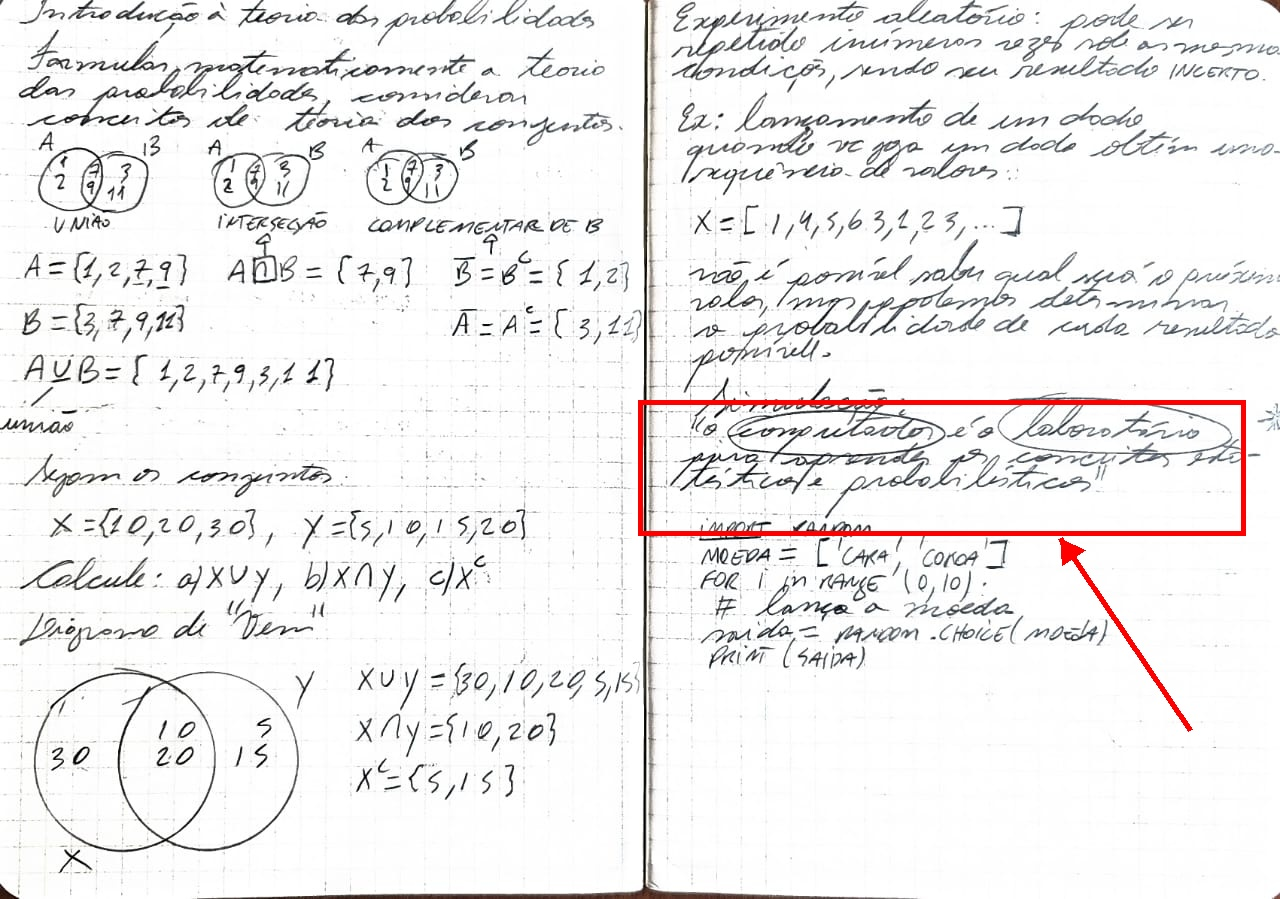
\includegraphics[width=0.7\textwidth]{figuras/cap.1/caderno_quadro.jpg}
  \caption[Anotação de caderno de campo de 28 de julho de 2025]{Anotação do meu caderno de campo de 28 de julho de 2025 durante o curso \textit{Fundamentos de Probabilidade e Estatística para Ciência de Dados} (ICMC-USP, Prof.~Dr. Francisco~A. Rodrigues). O quadro destaca a frase: \enquote{Simulação: `o computador é o laboratório para aprender os conceitos estatísticos e probabilísticos'.} As palavras \enquote{computador} e \enquote{laboratório} estão circuladas.}
  \label{fig:caderno-rodrigues}
\end{figure}

O nível de letramento técnico necessário varia conforme o objeto de estudo: investigações focadas nas práticas de pesquisa em inteligência artificial, como foi meu caso, exigem conhecimento aprofundado. A necessidade de letramento que experimentei encontra eco em debates dentro da própria ciência da computação. \textcite{Wallach2014} formula pergunta que espelha, desde dentro do campo, o que a ecologia das práticas de Stengers permite nomear de fora: poucos cientistas da computação desenvolveriam modelos para analisar dados astronômicos sem envolver astrônomos; por que, então, tantos métodos para analisar dados sociais são desenvolvidos sem o envolvimento de cientistas sociais? A resposta de Wallach é que temos intuições fortes sobre o mundo social, e essas intuições nos fazem crer que compreendemos fenômenos sociais sem precisar de formação específica. Intuição, porém, escapa à descrição como análise. O argumento de Wallach é estrutural: a colaboração precisa ser séria, no modo de criar equipes genuinamente interdisciplinares, em lugar do modo de convocar um cientista social para cada cem cientistas da computação. Nos termos da ecologia das práticas, o que Wallach identifica é que a prática de construção de sistemas que tomam o social como objeto exige, quando levada a sério, o envolvimento de quem conhece esse objeto com seus próprios requisitos, e não apenas como variável a modelar. O diagnóstico converge com o que \textcite{Vicentin_2022_Esboco} formula a partir de Simondon: sem a conexão entre o fazer técnico e o conhecimento sócio-histórico, a tecnologia permanece aquém de sua ética imanente, limitada a reproduzir estruturas existentes em lugar de realizar o potencial transformador que o aprofundamento técnico abre.

O argumento desta compostagem pode agora ser reunido. O momento de que parti produziu fricção, e a fricção revelou que a prática de pesquisa em IA e a da etnografia têm requisitos que não se traduzem por um critério comum. Minha resposta foi habitar essa fricção: buscar letramento técnico suficiente para acompanhar os pesquisadores em seus próprios termos, sem com isso pretender que a diferença entre as práticas se dissolvesse ou que eu me tornasse pesquisadora de computação. Stengers descreve essa aposta com o conceito de \emph{wager}: a aposta de que coletivos com preocupações distintas podem entrar em novas relações simbióticas se souberem aprender uns com os encontros com os outros \parencite[p.~103--104]{stengers2018another}. O letramento foi, nesse sentido, a forma que essa aposta tomou na minha pesquisa, um modo de sustentar o encontro entre práticas com exigências distintas que não se confunde com rendição nem com denúncia, e que transformou a fricção em fermentação.\footnote{O letramento que defendo aqui guarda uma ambiguidade quando passa do meu caso, o da pesquisadora cujo objeto é a própria IA, para a narrativa mais ampla do \emph{AI literacy} dirigida ao usuário leigo de IA generativa. Aprender a usar esses sistemas é exigência legítima de quem quer usá-los com autonomia crítica; a mesma exigência, porém, serve de álibi quando erros estruturais dos sistemas, as alucinações e os vieses que não dependem da perícia de quem usa, são reinterpretados como incompetência do usuário. Reconhecer essa ambiguidade não cancela a exigência do letramento; impede que ela desresponsabilize quem produz os sistemas. Desenvolvo a face técnica desse argumento na seção~\ref{sec:etnografias_ia_mediacao} do capítulo~\ref{capitulo2}, onde distingo o que está nas mãos dos desenvolvedores do que está nas mãos dos usuários.}

\subsection{Compostando a política: ciência como captação de recursos}
\label{subsec:compostagem4}

De todas as compostagens, esta foi talvez a mais imediata, embora tenha sido a última a se formular como tal. Preciso ser franca sobre algo que me acompanhou durante boa parte do trabalho de campo: irritação surda, difícil de formular na época, com o fato de que eu não via a inteligência artificial sendo feita, ao menos como eu imaginava. Eu havia me proposto a fazer uma etnografia de um centro de pesquisa em IA, e os leitores de uma tese como esta esperariam, com razão, saber como a inteligência artificial é produzida. O que eu encontrava, contudo, era outra coisa: eventos de difusão científica, negociações de financiamento, apresentações a parceiros corporativos, disputas por infraestrutura computacional.
A pesquisa em IA parecia acontecer em outro lugar, sempre atrás de uma porta que eu não conseguia abrir, dentro de computadores aos quais eu não tinha acesso, em reuniões técnicas cujo vocabulário eu não dominava. O que eu tinha diante de mim era, como defendo nas compostagens anteriores, a própria construção da inteligência artificial. Eu apenas não a identificava dessa maneira, porque seguia em busca da ciência por trás de toda aquela política.

Assistia a Fábio apresentar o Centro em eventos de difusão e anotava \enquote{divulgação}, em lugar de \enquote{ciência}. Ouvia Cláudio explicar como navegava entre os três potes de recursos e classificava aquilo como \enquote{gestão}, em lugar de \enquote{pesquisa}. Quando Cláudio me descreveu em entrevista como, um mês antes de \textit{deadlines} de conferências, tornava-se impossível conseguir GPU no Centro, reconheci ali o mesmo padrão: eu teria classificado aquilo como \enquote{logística}, em lugar de decisão epistemológica. Na minha primeira visita ao Centro, parei diante da sala de TI sem compreender o que acontecia ali. Anos depois, percebi que aquele desconforto era sintomático de uma separação que eu carregava e que o campo insistia em desfazer. Eu procurava a inteligência artificial dentro dos computadores, nos códigos, nos modelos, e o que encontrava eram pessoas negociando, traduzindo interesses, reconfigurando alianças. A angústia era intelectual e profissional, e me perguntava com frequência como apresentar uma etnografia de um centro de inteligência artificial sem propriamente descrever como a IA é feita.

Essa frustração, contudo, era metodologicamente produtiva. Ela me sinalizava o ponto exato onde minhas categorias analíticas falhavam, onde o arranjo que eu trazia precisava ser reconfigurado. Law argumenta que o \textit{hinterland} de qualquer método se ramifica indefinidamente para além de laboratórios e protocolos, alcançando conhecimento tácito, \textit{software}, habilidades linguísticas, capacidades de gestão, sistemas de transporte e comunicação, escalas salariais, fluxos de financiamento, prioridades de agências de fomento e agendas abertamente políticas e econômicas \parencite[pp.~41--42]{Law2004After}. O que eu observava no \texttt{C4AI} (as sessões de \textit{Design Thinking} que costuravam critérios da USP, \texttt{IBM} e Brasil; a venda da divisão de saúde da \texttt{IBM} que redirecionava linhas de pesquisa; as disputas por GPU que se tornavam decisões epistemológicas; Fábio apresentando em Bluetalks como parte do fazer ciência) era precisamente esse \textit{hinterland} ramificado que métodos convencionais relegam à invisibilidade.

Law descreve \textit{method assemblage} como produção de feixe de relações ramificadas que gera presença, ausência manifesta e \textit{otherness} \parencite[p.~84]{Law2004After}. No meu caso: a presença esperada era a ciência sendo feita (códigos, modelos, experimentos); a ausência manifesta eram as negociações que eu sabia serem necessárias e classificava como \enquote{entorno}; e a \textit{otherness} era precisamente o trabalho de captação de recursos que precisava desaparecer para que a ciência aparecesse como autônoma. Minha frustração era sintoma de que minhas categorias prévias produziam exatamente essa divisão entre presença, ausência e \textit{otherness}. O que o campo me obrigou a fazer foi reconfigurar essas fronteiras: reconhecer que o que eu havia relegado à \textit{otherness} era constitutivo da presença.

A pergunta \enquote{onde está a ciência que esses recursos sustentam?} pressupunha a separação entre ciência e política que o próprio campo tratava de desmentir. Captar recursos, negociar parcerias, justificar investimentos perante agências de fomento e corporações transnacionais é a pesquisa ela mesma. A pergunta não encontrou resposta; perdeu sentido.

A dificuldade em reconhecer aquelas atividades como fazer IA era expressão concreta da alienação técnica discutida anteriormente: a separação entre o que seria estritamente técnico e o que seria entorno da pesquisa reproduz a cisão que impede o amadurecimento da tecnologia. O que o campo me obrigou a compreender, por vias etnográficas, foi que as negociações de financiamento, as disputas por GPU, as apresentações a parceiros corporativos eram parte constitutiva da individuação técnica da IA.

Essa inseparabilidade entre ciência e política era o que o campo me dava a ver quando eu conseguia suspender a distinção prévia. Os próprios projetos de pesquisa do Centro foram definidos, como Fábio me relata, por sessões de \textit{Design Thinking} em que três critérios precisavam se alinhar simultaneamente: a USP teria liderança científica no tema, a \texttt{IBM} teria interesse na temática, e o Brasil teria diferencial internacional. A decisão era uma só, e nela se fundiam avaliação epistêmica, estratégia corporativa e posicionamento geopolítico, sem que houvesse momento científico de escolha de tema seguido de momento político de negociação de recursos.\footnote{Os relatórios internos do \texttt{C4AI} documentam esse processo: o grupo de \textit{Design Thinking} organizou quatro reuniões com mais de 80 pesquisadores, convergindo em cinco desafios. O critério exigia que os resultados fossem estratégicos para o Brasil, relevantes para USP e \texttt{IBM} e com alto potencial de inovação. A partir de 2022, quando a \texttt{IBM} vendeu Watson Health, o Centro decidiu não enfatizar esforços relacionados a saúde; quando o grupo AgriBio conquistou financiamento independente (INCT), tornou-se autossuficiente em relação aos recursos do \texttt{C4AI}. Em ambos os casos, a reconfiguração não separava decisão científica de decisão política.}

Quando a \texttt{IBM} vendeu sua divisão de saúde, o Centro parou de investir diretamente em pesquisa de IA em saúde. Quando a \texttt{IBM} saiu de agronegócio, o mesmo ocorreu. As reorientações de pesquisa se davam como reconfigurações da rede em que agenda científica e interesse corporativo constituíam, desde a origem, um único arranjo, em lugar de imposições externas sobre uma agenda científica autônoma.

Do mesmo modo, quando Fábio apresentava resultados em eventos como as Bluetalks, estava recrutando aliados, fortalecendo a rede, traduzindo interesses de públicos heterogêneos para manter a cadeia de associações que tornava a pesquisa possível. Latour descreve precisamente esse trabalho como constitutivo da prática tecnocientífica: o que se perde ao separá-lo da ciência propriamente dita é justamente o que o torna ciência, ou seja, a capacidade de alistar e manter associados elementos heterogêneos \parencite{Latour2011CienciaEmAcao}. A junção dos termos técnica e ciência em \textit{tecnociência} é exigência empírica, e o campo que eu observava tornava essa exigência particularmente visível.

A agência, nessas reconfigurações, é distribuída pela rede: emerge das associações entre pesquisadores, instituições, infraestruturas, contratos, modelos computacionais e políticas de fomento. Nenhum desses elementos age sozinho ou determina sozinho o curso da pesquisa. Quando o \texttt{C4AI} delega a definição de temas de pesquisa a sessões de \textit{Design Thinking} que costuram simultaneamente critérios da USP, da \texttt{IBM} e do Brasil, a agência dessa decisão reside na associação entre os participantes, e cada reconfiguração da rede redistribui a agência por novas cadeias de translação.

O cenário contemporâneo de investimentos massivos em inteligência artificial (com a concentração de capacidade computacional em poucas corporações, a corrida geopolítica por soberania tecnológica e a crescente dependência de infraestruturas de alto custo) torna essas dinâmicas particularmente visíveis. Resta saber se a pesquisa em IA é caso em que a inseparabilidade entre ciência e política se intensifica a ponto de exigir novos instrumentos analíticos, ou se apenas torna mais difícil ignorar o que Latour já descrevia em outros campos, quando os investimentos eram menores e as redes, menos extensas.

\section{Arremate: etnografias e compostagens}
\label{sec:conclusoes-cap1}

Este capítulo funcionou como laboratório de suas próprias decisões. Começou pela pergunta sobre onde está o laboratório dos pesquisadores de IA do \texttt{C4AI}, e a resposta me exigiu um conjunto de movimentos que o próprio capítulo inscreveu enquanto os realizava: deslocar minha expectativa do laboratório centralizado para o laboratório disperso e portátil, reconhecer a inteligência artificial como ciência em construção em lugar de objeto consolidado, e aceitar que a etnografia de uma rede tecnocientífica desse tipo se faz por composição de materiais heterogêneos, em lugar de descrição linear de um lugar único.

Recapitulo o percurso seção por seção antes de reuni-lo. Abri o capítulo com a pergunta sobre onde está o laboratório dos pesquisadores de inteligência artificial e onde estão os seus cientistas, e parti da fotografia da entrega do primeiro supercomputador à \texttt{OpenAI} em 2016 para situar a infraestrutura computacional como condição de entrada do campo; a resposta deslocou a minha expectativa de um laboratório centralizado para um laboratório disperso e portátil, e firmou a inteligência artificial como ciência em construção, e não como objeto consolidado. Na seção sobre etnografia heterodoxa, articulei a teoria ator-rede de Latour à etnografia de Kofes para sustentar que o método se ensaia enquanto se experimenta, e mostrei que as duas abordagens enfrentam o mesmo problema por vias distintas, a de seguir os actantes e a de deixar-se afetar pelo encontro de campo, o que me autorizou a tomar a própria tese como inscrição tecnocientífica que faz redes ao descrevê-las.

Na seção sobre cortar e costurar redes, tratei o corte como a operação que delimita uma rede que de outro modo se daria a ver como infinita, e reuni cinco modos do corte (Strathern, Barad, Haraway, Costa e Law) para descrever os quatro cortes que cada capítulo da tese faz, cada um pela tríade de Law (presença, ausência manifesta e \textit{otherness}) e legível como \textit{enactment} no sentido de Mol; recuperei ali a etimologia de \textit{contexto} como \textit{contexere}, tecer junto, para fazer trabalhar em português a relacionalidade têxtil que Law nomeia com \textit{hinterland}. Na seção sobre o \textit{patchwork}, desenvolvi a figuração têxtil do método pelo \textit{crazy quilt}, em que a heterogeneidade dos retalhos, a visibilidade das costuras e a recusa de um padrão geral correspondem ponto a ponto ao que a tese precisa fazer ao compor materiais heterogêneos, e diferenciei a minha posição da malha de Ingold, que recusa o corte, para ficar com Strathern e Haraway, para quem cortar é condição da descrição.

Na seção sobre existências parciais, parti do princípio de simetria de Latour e o desdobrei até as existências parciais, organizando os conceitos da seção (híbrido, quase-máquina, agência distribuída, conexão parcial, fazer-com) por uma grade de três planos, substância, propriedade e efeito-relação, que converge para o eixo de que a relação constitui; descrevi os sistemas de inteligência artificial generativa como máquinas e, na leitura que faço de Latour, também como quase-máquinas no plano do efeito-relação, reconheci o \texttt{claude} como objeto múltiplo, e tratei os instrumentos de inscrição da tese como actantes que se compõem comigo. Na subseção sobre por que fazer parentesco com este problema, sustentei que o meu fazer-com a inteligência artificial generativa é escolha metodológica deliberada de ficar com um companheiro problemático, e documentei essa escolha com a sequência de três capturas de tela de uma conversa de revisão com o \texttt{claude}, em que a régua estilística do modelo é contestada, recua e se reformula, e a agência epistêmica se redistribui turno a turno. Na passagem cosmotécnica, situei o fazer-com entre uma antropóloga brasileira e um modelo treinado predominantemente em dados anglófonos como gesto cosmotécnico particular, no sentido de Hui.

Na subseção em que defini a tecno-etnografia, distingui-a da etnografia digital de Pink, Horst e Postill por uma inflexão, a de fazer a pesquisa não só \textit{sobre}, mas \textit{com} a inteligência artificial generativa, tomada ao mesmo tempo como objeto e como dado, com auditabilidade pública das técnicas nos repositórios do \texttt{GitHub} como contraparte material e ética desse compromisso; e produzi, como demonstração, seis inscrições do próprio capítulo, três sincrônicas que respondem ao que se liga a quê na minha escrita e três diacrônicas que respondem a quando cada conceito entra, persiste e migra, das quais retive que a minha costura argumentativa ainda se apoia em palavras genéricas a teorizar e que a conexão entre as ciências sociais e o par humano-máquina-método é a \textit{otherness} que ainda preciso fazer trabalhar. Na seção sobre compostagens, nomeei quatro fermentações de materiais que o desenho inicial da pesquisa mantinha separados, a do método (a regra de estudar a ciência em construção com a dispersão da pesquisa em inteligência artificial), a da teoria (a simetria que se decompôs em existências parciais no próprio trabalho de campo), a do letramento (a minha formação em ciências sociais com o letramento técnico que o campo me exigiu, depois de pesquisadores da computação contestarem os conceitos de Pasquinelli e Crawford que levei a uma aula) e a da política (a separação prévia entre ciência e política desfeita pela evidência de que a pesquisa no \texttt{C4AI} é, ao mesmo tempo, decisão epistêmica e captação de recursos).

Três gestos analíticos se desdobraram a partir dessa pergunta inicial. O primeiro foi nomear cortes, ou seja, os gestos de delimitação que tornam descritível uma rede que se desdobra indefinidamente.
A subseção \enquote{Cortando redes} convocou o corte de Strathern e conceitos vizinhos de Barad, Haraway, Costa e Law para descrever como cada capítulo desta tese faz um corte específico: reflexivo no capítulo~\ref{capitulo1}, teórico no capítulo~\ref{capitulo2}, pela extensão no capítulo~\ref{capitulo3} e pela densidade no capítulo~\ref{capitulo4}. Os quatro cortes funcionam como \textit{enactments} no sentido praxiográfico que Mol e Law desenvolvem, e os quatro capítulos performam o \texttt{C4AI} como quatro objetos etnográficos que se atravessam sem se subsumir uns aos outros.

O segundo gesto foi descrever o fazer-com a inteligência artificial generativa que minha tese assume como dado etnográfico, em lugar de recurso técnico secundário. A seção \enquote{Existências parciais} desdobrou um movimento teórico interno à obra de Latour, do princípio de simetria como ponto de partida à formulação das existências parciais como descrição mais precisa do que o campo me apresentava. Esse movimento gerou três contribuições. A noção de quase-máquina, que tomo de Latour como leitura e não como definição, me permitiu descrever esses sistemas, que são máquinas, também como entidades abertas e parcialmente conectadas, que escapam à partição entre humano e não humano. A noção de agência distribuída descreveu o mecanismo pelo qual essas existências parciais agem juntas, redistribuindo a responsabilidade pela ação por cadeias de translação. A multiplicidade ontológica de Law me permitiu reconhecer o \texttt{claude} como objeto múltiplo (em treinamento, em \textit{deployment}, em auditoria, em uso), e cada Claude existe como fazer-com situado com quem o aciona, em lugar de objeto singular acessível a todos.

O terceiro gesto foi figurar as transformações recíprocas que tornaram minha pesquisa possível. A seção \enquote{Compostagens} nomeou quatro misturas específicas de materiais heterogêneos que precisaram fermentar juntos para que a descrição se tornasse possível: a regra latouriana de estudar a ciência em construção fermentando com a dispersão característica da pesquisa em IA; a simetria metodológica fermentando com a especificidade da inteligência artificial generativa para gerar existências parciais; minha formação em ciências sociais fermentando com o letramento técnico que o campo me exigiu; e a separação prévia entre ciência e política fermentando com a evidência empírica de que a pesquisa em IA, no \texttt{C4AI}, é simultaneamente decisão epistêmica e captação de recursos. Cada compostagem inscreve um momento em que a descrição etnográfica exigiu decompor partições prévias e tolerar a fermentação de materiais que o desenho inicial da pesquisa mantinha separados.

O que sustenta este capítulo é, antes de teórico, etnográfico, e ele me deixou com uma questão que carrego pela tese inteira e que prefiro não fechar aqui. Penso e construo o argumento por uma figuração têxtil, em que o trabalho de pesquisa se faz de fios, tramas, costuras, nós e cortes, e ao mesmo tempo inscrevo o seu percurso em diagramas, gráficos e textos-mapa que disponho ao longo do capítulo para dar a ver, numa superfície plana, o que de outro modo se perderia na dispersão. São duas figurações que constituem esta tese, e que vim a reconhecer como figurações topológicas, no sentido em que a própria teoria ator-rede é topológica: a rede de \textcite{latour1996clarifications}, que retomei na subseção~\ref{subsec:cortando-redes}, tem caráter fibroso, feito de fios e laços tecidos, e a força dela vem do tecer cuidadoso de laços fracos. A rede de Latour é, ela própria, um tecido, e por isso rede e trama não são figurações opostas, e sim homólogas sem serem homogêneas: as duas são feitas de fios e nós, mas de materiais distintos e em formas distintas de apresentação, a rede que recruta e vence em Latour e a trama que oferece e fica-com em Haraway. É essa homologia que sustenta a passagem deste capítulo aos capítulos~\ref{capitulo3} e~\ref{capitulo4}, em que faço, corto e sigo redes, porque a rede que descrevo no campo e a trama com que escrevo a tese são o mesmo gesto têxtil em fios de matéria diferente.

A mesma topologia, porém, separa duas ordens de cognição. Pensar em rede é pensar topologicamente, em nós de tantas dimensões quantas forem as suas conexões, o que nenhuma superfície plana comporta; mostrar uma rede é fácil, basta conectar os nós numa superfície de duas dimensões. A figuração têxtil, com que penso, pertence à primeira ordem, e os textos-mapa, com que inscrevo, à segunda, e por isso a têxtil não aparece nas figuras: ela é o pensamento que produz as figuras, e não uma das figuras. A compostagem que desdobrei na seção sobre as fermentações é, do mesmo modo, figuração do pensamento, e não da inscrição, porque fermentar materiais heterogêneos para que se transformem uns nos outros é um modo de pensar com eles no tempo, da mesma ordem do tecer, e tampouco se deixa mostrar numa superfície: o que um diagrama exibiria seria o resultado da mistura, não o fermentar que a fez. Demorei a reconhecer que a figuração têxtil não podia ser desenhada, e que essa impossibilidade não era falha minha nem da figura, e sim a natureza de cada uma. Um mapa mostra nós e conexões, isto é, as coisas já postas em relação; não mostra o relacionar que as pôs assim, e é esse relacionar que a trama pensa. A relação, como sustento desde a subseção~\ref{subsec:cortando-redes} a partir de Strathern, nunca está dada, e se refaz a cada corte e a cada costura que escolho fazer, e a superfície da inscrição só recebe o resultado da relação, não a relação em ato.

Habito, nesse ponto, uma tensão que não chega a ser contradição, e é dela que esta tese se faz: pratico na escrita um modo de pensamento que não cabe na superfície em que inscrevo os textos-mapa, e os dois coexistem sem que um se reduza ao outro. A coexistência das duas figurações, em lugar da escolha entre elas, é parte do que proponho, e as duas mexem com sentidos distintos, o tato e o tempo do raciocínio que se tece, e a visão que apreende de uma só vez a superfície plana. Deixo a questão aberta para os capítulos seguintes, sem a pretensão de resolvê-la: se a figuração têxtil é um modo de pensar, e se o que reúne as coisas é uma relação que nunca está dada, como se pensa por tramas, como se mostra esse pensar numa superfície que só recebe o que já foi tecido, e o que acontece quando ponho em questão a própria diferença entre tecer um argumento e mapeá-lo.
O método se ensaiou enquanto se experimentava, conforme a orientação de \textcite{Kofes2015Maconaria}, e os conceitos que convoquei foram chamados pelo que o campo exigia. Esse percurso me autoriza um gesto que executei de modo recursivo neste capítulo~\ref{capitulo1}: aplicar à própria escrita da tese o tratamento que aplico aos pesquisadores que descrevo. A subseção \enquote{Tecnoetnografia} converteu o texto deste capítulo em grafo de co-ocorrências e leu suas comunidades como tópicos latentes, inscrevendo as costuras conseguidas e as fissuras pendentes. A subseção \enquote{Por que fazer parentesco com este problema?} documentou em sequência de capturas de tela uma cena de fazer-com o \texttt{claude} durante a revisão deste mesmo capítulo. Em ambos os casos, minha tese funciona como inscrição tecnocientífica que se deixa medir pelos mesmos instrumentos com que se compromete a medir o \texttt{C4AI}, e a reflexividade metodológica assume a forma de gesto recursivo, em lugar de declaração externa sobre a relação entre quem pesquisa e objeto.

O que este capítulo deixou em aberto é o desdobramento da tecno-etnografia nas três tramas que organizam os capítulos seguintes. Cada uma delas retoma, em escala e materialidade próprias, os três gestos analíticos que este capítulo desenvolveu sobre a sua própria escrita: o corte que delimita a rede para torná-la descritível, a compostagem que põe materiais heterogêneos a fermentar juntos, e a descrição das existências parciais que se compõem na pesquisa. O que o capítulo~\ref{capitulo1} entrega aos capítulos etnográficos é a consciência de que a figuração com que se descreve a tecnociência é parte do que se descreve, e que essa figuração precisa ser assumida em vez de naturalizada, e não um sumário do que cada um fará.

Esse legado tem consequências diretas para o que esta tese pode descrever nos capítulos seguintes. Se eu deixasse o trabalho sobre as figurações implícito, descreveria o \texttt{C4AI} no capítulo~\ref{capitulo3} e o \texttt{Spira} no capítulo~\ref{capitulo4} usando, sem perceber, o vocabulário militar-industrial em que Latour formulou a tecnociência, isto é, alistar aliados, recrutar para vencer, mobilizar provas de força, sustentar a máquina de guerra das publicações e dos consórcios. Esse vocabulário não é falso, é figuração específica, e está admitida pelo próprio Latour como mudança de metáforas que contaminou o trabalho descritivo, conforme retomo no capítulo~\ref{capitulo2}. O que faço neste capítulo~\ref{capitulo1}, e adenso no próximo, é abrir o espaço para descrições da tecnociência em outros vocabulários, isto é, descrições que mobilizam costuras de retalho com Strathern, compostagens e tornar-se-com com Haraway, aliar e oferecer com Stengers, e ficar com o problema sem a pretensão de resolvê-lo. As três tramas seguintes, somadas a este capítulo~\ref{capitulo1} que se ofereceu como laboratório de suas próprias decisões, compõem o que esta tese chama de tecno-etnografia, e ocupam, cada uma a seu modo, esse espaço aberto.